\documentclass[twoside]{book}

% Packages required by doxygen
\usepackage{fixltx2e}
\usepackage{calc}
\usepackage{doxygen}
\usepackage{graphicx}
\usepackage[utf8]{inputenc}
\usepackage{makeidx}
\usepackage{multicol}
\usepackage{multirow}
\PassOptionsToPackage{warn}{textcomp}
\usepackage{textcomp}
\usepackage[nointegrals]{wasysym}
\usepackage[table]{xcolor}

% Font selection
\usepackage[T1]{fontenc}
\usepackage{mathptmx}
\usepackage[scaled=.90]{helvet}
\usepackage{courier}
\usepackage{amssymb}
\usepackage{sectsty}
\renewcommand{\familydefault}{\sfdefault}
\allsectionsfont{%
  \fontseries{bc}\selectfont%
  \color{darkgray}%
}
\renewcommand{\DoxyLabelFont}{%
  \fontseries{bc}\selectfont%
  \color{darkgray}%
}
\newcommand{\+}{\discretionary{\mbox{\scriptsize$\hookleftarrow$}}{}{}}

% Page & text layout
\usepackage{geometry}
\geometry{%
  a4paper,%
  top=2.5cm,%
  bottom=2.5cm,%
  left=2.5cm,%
  right=2.5cm%
}
\tolerance=750
\hfuzz=15pt
\hbadness=750
\setlength{\emergencystretch}{15pt}
\setlength{\parindent}{0cm}
\setlength{\parskip}{0.2cm}
\makeatletter
\renewcommand{\paragraph}{%
  \@startsection{paragraph}{4}{0ex}{-1.0ex}{1.0ex}{%
    \normalfont\normalsize\bfseries\SS@parafont%
  }%
}
\renewcommand{\subparagraph}{%
  \@startsection{subparagraph}{5}{0ex}{-1.0ex}{1.0ex}{%
    \normalfont\normalsize\bfseries\SS@subparafont%
  }%
}
\makeatother

% Headers & footers
\usepackage{fancyhdr}
\pagestyle{fancyplain}
\fancyhead[LE]{\fancyplain{}{\bfseries\thepage}}
\fancyhead[CE]{\fancyplain{}{}}
\fancyhead[RE]{\fancyplain{}{\bfseries\leftmark}}
\fancyhead[LO]{\fancyplain{}{\bfseries\rightmark}}
\fancyhead[CO]{\fancyplain{}{}}
\fancyhead[RO]{\fancyplain{}{\bfseries\thepage}}
\fancyfoot[LE]{\fancyplain{}{}}
\fancyfoot[CE]{\fancyplain{}{}}
\fancyfoot[RE]{\fancyplain{}{\bfseries\scriptsize Generated on Sat Jan 31 2015 18\+:38\+:50 for g\+P\+H by Doxygen }}
\fancyfoot[LO]{\fancyplain{}{\bfseries\scriptsize Generated on Sat Jan 31 2015 18\+:38\+:50 for g\+P\+H by Doxygen }}
\fancyfoot[CO]{\fancyplain{}{}}
\fancyfoot[RO]{\fancyplain{}{}}
\renewcommand{\footrulewidth}{0.4pt}
\renewcommand{\chaptermark}[1]{%
  \markboth{#1}{}%
}
\renewcommand{\sectionmark}[1]{%
  \markright{\thesection\ #1}%
}

% Indices & bibliography
\usepackage{natbib}
\usepackage[titles]{tocloft}
\setcounter{tocdepth}{3}
\setcounter{secnumdepth}{5}
\makeindex

% Hyperlinks (required, but should be loaded last)
\usepackage{ifpdf}
\ifpdf
  \usepackage[pdftex,pagebackref=true]{hyperref}
\else
  \usepackage[ps2pdf,pagebackref=true]{hyperref}
\fi
\hypersetup{%
  colorlinks=true,%
  linkcolor=blue,%
  citecolor=blue,%
  unicode%
}

% Custom commands
\newcommand{\clearemptydoublepage}{%
  \newpage{\pagestyle{empty}\cleardoublepage}%
}


%===== C O N T E N T S =====

\begin{document}

% Titlepage & ToC
\hypersetup{pageanchor=false,
             bookmarks=true,
             bookmarksnumbered=true,
             pdfencoding=unicode
            }
\pagenumbering{roman}
\begin{titlepage}
\vspace*{7cm}
\begin{center}%
{\Large g\+P\+H \\[1ex]\large 0.\+0.\+1 }\\
\vspace*{1cm}
{\large Generated by Doxygen 1.8.8}\\
\vspace*{0.5cm}
{\small Sat Jan 31 2015 18:38:50}\\
\end{center}
\end{titlepage}
\clearemptydoublepage
\tableofcontents
\clearemptydoublepage
\pagenumbering{arabic}
\hypersetup{pageanchor=true}

%--- Begin generated contents ---
\chapter{Main Page}
\label{index}\hypertarget{index}{}\input{index}
\chapter{Hierarchical Index}
\section{Class Hierarchy}
This inheritance list is sorted roughly, but not completely, alphabetically\+:\begin{DoxyCompactList}
\item \contentsline{section}{Action}{\pageref{classAction}}{}
\item \contentsline{section}{Argument\+Frame}{\pageref{classArgumentFrame}}{}
\item \contentsline{section}{Choix\+Ligne}{\pageref{classChoixLigne}}{}
\item exception\begin{DoxyCompactList}
\item \contentsline{section}{exception\+\_\+base}{\pageref{structexception__base}}{}
\begin{DoxyCompactList}
\item \contentsline{section}{gv\+\_\+error}{\pageref{structgv__error}}{}
\begin{DoxyCompactList}
\item \contentsline{section}{subgraph\+\_\+not\+\_\+found}{\pageref{structsubgraph__not__found}}{}
\end{DoxyCompactList}
\item \contentsline{section}{io\+\_\+error}{\pageref{structio__error}}{}
\begin{DoxyCompactList}
\item \contentsline{section}{file\+\_\+not\+\_\+exist}{\pageref{structfile__not__exist}}{}
\item \contentsline{section}{not\+\_\+regular\+\_\+file}{\pageref{structnot__regular__file}}{}
\item \contentsline{section}{wrong\+\_\+import\+\_\+file}{\pageref{structwrong__import__file}}{}
\end{DoxyCompactList}
\item \contentsline{section}{ph\+\_\+error}{\pageref{structph__error}}{}
\begin{DoxyCompactList}
\item \contentsline{section}{process\+\_\+not\+\_\+found}{\pageref{structprocess__not__found}}{}
\item \contentsline{section}{process\+\_\+required}{\pageref{structprocess__required}}{}
\item \contentsline{section}{sort\+\_\+not\+\_\+found}{\pageref{structsort__not__found}}{}
\end{DoxyCompactList}
\item \contentsline{section}{ph\+\_\+parse\+\_\+error}{\pageref{structph__parse__error}}{}
\begin{DoxyCompactList}
\item \contentsline{section}{pint\+\_\+phc\+\_\+crash}{\pageref{structpint__phc__crash}}{}
\item \contentsline{section}{text\+Area\+Empty\+\_\+exception}{\pageref{structtextAreaEmpty__exception}}{}
\end{DoxyCompactList}
\item \contentsline{section}{pint\+\_\+program\+\_\+not\+\_\+found}{\pageref{structpint__program__not__found}}{}
\end{DoxyCompactList}
\end{DoxyCompactList}
\item exception\begin{DoxyCompactList}
\item \contentsline{section}{exception\+\_\+base}{\pageref{structexception__base}}{}
\end{DoxyCompactList}
\item \contentsline{section}{Func\+Frame}{\pageref{classFuncFrame}}{}
\item \contentsline{section}{G\+Action}{\pageref{classGAction}}{}
\item \contentsline{section}{G\+Process}{\pageref{classGProcess}}{}
\item \contentsline{section}{G\+V\+Edge}{\pageref{structGVEdge}}{}
\item \contentsline{section}{G\+V\+Node}{\pageref{structGVNode}}{}
\item \contentsline{section}{G\+V\+Skeleton\+Graph}{\pageref{classGVSkeletonGraph}}{}
\item \contentsline{section}{I\+O}{\pageref{classIO}}{}
\item \contentsline{section}{P\+H}{\pageref{classPH}}{}
\item \contentsline{section}{P\+H\+I\+O}{\pageref{classPHIO}}{}
\item \contentsline{section}{Process}{\pageref{classProcess}}{}
\item Q\+Dialog\begin{DoxyCompactList}
\item \contentsline{section}{Connection\+Settings}{\pageref{classConnectionSettings}}{}
\item \contentsline{section}{Function\+Form}{\pageref{classFunctionForm}}{}
\item \contentsline{section}{Tikz\+Editor}{\pageref{classTikzEditor}}{}
\end{DoxyCompactList}
\item Q\+Graphics\+Rect\+Item\begin{DoxyCompactList}
\item \contentsline{section}{G\+Sort}{\pageref{classGSort}}{}
\end{DoxyCompactList}
\item Q\+Graphics\+Scene\begin{DoxyCompactList}
\item \contentsline{section}{P\+H\+Scene}{\pageref{classPHScene}}{}
\end{DoxyCompactList}
\item Q\+Graphics\+View\begin{DoxyCompactList}
\item \contentsline{section}{My\+Area}{\pageref{classMyArea}}{}
\end{DoxyCompactList}
\item Q\+Main\+Window\begin{DoxyCompactList}
\item \contentsline{section}{Main\+Window}{\pageref{classMainWindow}}{}
\end{DoxyCompactList}
\item Q\+Object\begin{DoxyCompactList}
\item \contentsline{section}{P\+H\+I\+O\+Test}{\pageref{classPHIOTest}}{}
\end{DoxyCompactList}
\item Q\+Syntax\+Highlighter\begin{DoxyCompactList}
\item \contentsline{section}{Colorer\+Sequences}{\pageref{classColorerSequences}}{}
\end{DoxyCompactList}
\item Q\+Text\+Edit\begin{DoxyCompactList}
\item \contentsline{section}{Text\+Area}{\pageref{classTextArea}}{}
\end{DoxyCompactList}
\item Q\+Widget\begin{DoxyCompactList}
\item \contentsline{section}{Area}{\pageref{classArea}}{}
\item \contentsline{section}{Tree\+Area}{\pageref{classTreeArea}}{}
\end{DoxyCompactList}
\item \contentsline{section}{Sort}{\pageref{classSort}}{}
\end{DoxyCompactList}

\chapter{Class Index}
\section{Class List}
Here are the classes, structs, unions and interfaces with brief descriptions\+:\begin{DoxyCompactList}
\item\contentsline{section}{\hyperlink{classAction}{Action} \\*Represents an \hyperlink{classAction}{Action} of the process hitting }{\pageref{classAction}}{}
\item\contentsline{section}{\hyperlink{classArea}{Area} \\*New Tab extends Q\+Widget }{\pageref{classArea}}{}
\item\contentsline{section}{\hyperlink{classArgumentFrame}{Argument\+Frame} }{\pageref{classArgumentFrame}}{}
\item\contentsline{section}{\hyperlink{classChoixLigne}{Choix\+Ligne} }{\pageref{classChoixLigne}}{}
\item\contentsline{section}{\hyperlink{classColorerSequences}{Colorer\+Sequences} }{\pageref{classColorerSequences}}{}
\item\contentsline{section}{\hyperlink{classConnectionSettings}{Connection\+Settings} }{\pageref{classConnectionSettings}}{}
\item\contentsline{section}{\hyperlink{structexception__base}{exception\+\_\+base} \\*Struct defining the base of the exception }{\pageref{structexception__base}}{}
\item\contentsline{section}{\hyperlink{structfile__not__exist}{file\+\_\+not\+\_\+exist} \\*Struct defining the exception called when the file does not exist extends \hyperlink{structio__error}{io\+\_\+error} }{\pageref{structfile__not__exist}}{}
\item\contentsline{section}{\hyperlink{classFuncFrame}{Func\+Frame} }{\pageref{classFuncFrame}}{}
\item\contentsline{section}{\hyperlink{classFunctionForm}{Function\+Form} }{\pageref{classFunctionForm}}{}
\item\contentsline{section}{\hyperlink{classGAction}{G\+Action} \\*Style and layout info to draw an action }{\pageref{classGAction}}{}
\item\contentsline{section}{\hyperlink{classGProcess}{G\+Process} \\*Style and layout info to draw a process }{\pageref{classGProcess}}{}
\item\contentsline{section}{\hyperlink{classGSort}{G\+Sort} \\*Style and layout info to draw a \hyperlink{classSort}{Sort} }{\pageref{classGSort}}{}
\item\contentsline{section}{\hyperlink{structgv__error}{gv\+\_\+error} \\*Struct defining the exception called when an error occurs in Graph\+Viz extends \hyperlink{structexception__base}{exception\+\_\+base} }{\pageref{structgv__error}}{}
\item\contentsline{section}{\hyperlink{structGVEdge}{G\+V\+Edge} \\*Struct containing the information for a G\+V\+Graph's edge }{\pageref{structGVEdge}}{}
\item\contentsline{section}{\hyperlink{structGVNode}{G\+V\+Node} \\*Struct containing the information for a G\+V\+Graph's node }{\pageref{structGVNode}}{}
\item\contentsline{section}{\hyperlink{classGVSkeletonGraph}{G\+V\+Skeleton\+Graph} \\*Object containing a libraph graph representing the skeleton (sorts+actions) of the model and its associated nodes and edges }{\pageref{classGVSkeletonGraph}}{}
\item\contentsline{section}{\hyperlink{classIO}{I\+O} \\*Manages the inputs and outputs at the lowest level }{\pageref{classIO}}{}
\item\contentsline{section}{\hyperlink{structio__error}{io\+\_\+error} \\*Struct defining the base of the \hyperlink{classIO}{I\+O} errors }{\pageref{structio__error}}{}
\item\contentsline{section}{\hyperlink{classMainWindow}{Main\+Window} \\*Builds the main window of the program extends Q\+Main\+Window }{\pageref{classMainWindow}}{}
\item\contentsline{section}{\hyperlink{classMyArea}{My\+Area} \\*Graph Widget extends Q\+Graphics\+View }{\pageref{classMyArea}}{}
\item\contentsline{section}{\hyperlink{structnot__regular__file}{not\+\_\+regular\+\_\+file} \\*Struct defining the exception called when the format of the file is not the one expected extends \hyperlink{structio__error}{io\+\_\+error} }{\pageref{structnot__regular__file}}{}
\item\contentsline{section}{\hyperlink{classPH}{P\+H} \\*Entire process hitting as defined in a \hyperlink{classPH}{P\+H} file }{\pageref{classPH}}{}
\item\contentsline{section}{\hyperlink{structph__error}{ph\+\_\+error} \\*Struct defining the exception called when there is an error in the \hyperlink{classPH}{P\+H} file extends \hyperlink{structexception__base}{exception\+\_\+base} }{\pageref{structph__error}}{}
\item\contentsline{section}{\hyperlink{structph__parse__error}{ph\+\_\+parse\+\_\+error} \\*Struct defining the exception called when the \hyperlink{classPH}{P\+H} file cannot be parsed extends \hyperlink{structexception__base}{exception\+\_\+base} }{\pageref{structph__parse__error}}{}
\item\contentsline{section}{\hyperlink{classPHIO}{P\+H\+I\+O} \\*Manages the inputs and outputs of the \hyperlink{classPH}{P\+H} files }{\pageref{classPHIO}}{}
\item\contentsline{section}{\hyperlink{classPHIOTest}{P\+H\+I\+O\+Test} \\*Checks that \hyperlink{classPH}{P\+H} files are parsed successfully }{\pageref{classPHIOTest}}{}
\item\contentsline{section}{\hyperlink{classPHScene}{P\+H\+Scene} \\*Graphic object representing the process hitting extends Q\+Graphics\+Scene }{\pageref{classPHScene}}{}
\item\contentsline{section}{\hyperlink{structpint__phc__crash}{pint\+\_\+phc\+\_\+crash} \\*Struct defining the exception called when Pint cannot be called extends \hyperlink{structph__parse__error}{ph\+\_\+parse\+\_\+error} }{\pageref{structpint__phc__crash}}{}
\item\contentsline{section}{\hyperlink{structpint__program__not__found}{pint\+\_\+program\+\_\+not\+\_\+found} \\*Struct defining the exception called when Pint is not found\$ extends \hyperlink{structexception__base}{exception\+\_\+base} }{\pageref{structpint__program__not__found}}{}
\item\contentsline{section}{\hyperlink{classProcess}{Process} \\*\hyperlink{classProcess}{Process} of the process hitting }{\pageref{classProcess}}{}
\item\contentsline{section}{\hyperlink{structprocess__not__found}{process\+\_\+not\+\_\+found} \\*Struct defining the exception called when the process called is not found extends \hyperlink{structph__error}{ph\+\_\+error} }{\pageref{structprocess__not__found}}{}
\item\contentsline{section}{\hyperlink{structprocess__required}{process\+\_\+required} \\*Struct defining the exception called when the process is not specified extends \hyperlink{structph__error}{ph\+\_\+error} }{\pageref{structprocess__required}}{}
\item\contentsline{section}{\hyperlink{classSort}{Sort} \\*\hyperlink{classSort}{Sort} of the process hitting }{\pageref{classSort}}{}
\item\contentsline{section}{\hyperlink{structsort__not__found}{sort\+\_\+not\+\_\+found} \\*Struct defining the exception called when the sort called are not found extends \hyperlink{structph__error}{ph\+\_\+error} }{\pageref{structsort__not__found}}{}
\item\contentsline{section}{\hyperlink{structsubgraph__not__found}{subgraph\+\_\+not\+\_\+found} \\*Struct defining the exception called when the subgraph is not found extends \hyperlink{structgv__error}{gv\+\_\+error} }{\pageref{structsubgraph__not__found}}{}
\item\contentsline{section}{\hyperlink{classTextArea}{Text\+Area} \\*Text Widget extends Q\+Text\+Edit }{\pageref{classTextArea}}{}
\item\contentsline{section}{\hyperlink{structtextAreaEmpty__exception}{text\+Area\+Empty\+\_\+exception} \\*Struct defining the exception called when the user update from an empty text\+Area extends \hyperlink{structph__parse__error}{ph\+\_\+parse\+\_\+error} }{\pageref{structtextAreaEmpty__exception}}{}
\item\contentsline{section}{\hyperlink{classTikzEditor}{Tikz\+Editor} }{\pageref{classTikzEditor}}{}
\item\contentsline{section}{\hyperlink{classTreeArea}{Tree\+Area} \\*Tree Wigets extends Q\+Widget }{\pageref{classTreeArea}}{}
\item\contentsline{section}{\hyperlink{structwrong__import__file}{wrong\+\_\+import\+\_\+file} }{\pageref{structwrong__import__file}}{}
\end{DoxyCompactList}

\chapter{File Index}
\section{File List}
Here is a list of all documented files with brief descriptions\+:\begin{DoxyCompactList}
\item\contentsline{section}{headers/\hyperlink{Action_8h}{Action.\+h} \\*Header for the \hyperlink{classAction}{Action} class }{\pageref{Action_8h}}{}
\item\contentsline{section}{headers/{\bfseries Area.\+h} }{\pageref{Area_8h}}{}
\item\contentsline{section}{headers/{\bfseries Argument\+Frame.\+h} }{\pageref{ArgumentFrame_8h}}{}
\item\contentsline{section}{headers/{\bfseries Colorer\+Sequences.\+h} }{\pageref{ColorerSequences_8h}}{}
\item\contentsline{section}{headers/{\bfseries Connection\+Settings.\+h} }{\pageref{ConnectionSettings_8h}}{}
\item\contentsline{section}{headers/\hyperlink{Exceptions_8h}{Exceptions.\+h} \\*Header for the Exceptions class }{\pageref{Exceptions_8h}}{}
\item\contentsline{section}{headers/{\bfseries Func\+Frame.\+h} }{\pageref{FuncFrame_8h}}{}
\item\contentsline{section}{headers/{\bfseries Function\+Form.\+h} }{\pageref{FunctionForm_8h}}{}
\item\contentsline{section}{headers/\hyperlink{GAction_8h}{G\+Action.\+h} \\*Header for the \hyperlink{classGAction}{G\+Action} class }{\pageref{GAction_8h}}{}
\item\contentsline{section}{headers/\hyperlink{GProcess_8h}{G\+Process.\+h} \\*Header for the \hyperlink{classGProcess}{G\+Process} class }{\pageref{GProcess_8h}}{}
\item\contentsline{section}{headers/\hyperlink{GSort_8h}{G\+Sort.\+h} \\*Header for the \hyperlink{classGSort}{G\+Sort} class }{\pageref{GSort_8h}}{}
\item\contentsline{section}{headers/\hyperlink{GVEdge_8h}{G\+V\+Edge.\+h} \\*Header for the \hyperlink{structGVEdge}{G\+V\+Edge} class }{\pageref{GVEdge_8h}}{}
\item\contentsline{section}{headers/\hyperlink{GVNode_8h}{G\+V\+Node.\+h} \\*Header for the \hyperlink{structGVNode}{G\+V\+Node} class }{\pageref{GVNode_8h}}{}
\item\contentsline{section}{headers/\hyperlink{GVSkeletonGraph_8h}{G\+V\+Skeleton\+Graph.\+h} \\*Header for the \hyperlink{classGVSkeletonGraph}{G\+V\+Skeleton\+Graph} class }{\pageref{GVSkeletonGraph_8h}}{}
\item\contentsline{section}{headers/\hyperlink{IO_8h}{I\+O.\+h} \\*Header for the \hyperlink{classIO}{I\+O} class }{\pageref{IO_8h}}{}
\item\contentsline{section}{headers/\hyperlink{MainWindow_8h}{Main\+Window.\+h} \\*Header for the Main class }{\pageref{MainWindow_8h}}{}
\item\contentsline{section}{headers/\hyperlink{MyArea_8h}{My\+Area.\+h} \\*Header for the \hyperlink{classMyArea}{My\+Area} class }{\pageref{MyArea_8h}}{}
\item\contentsline{section}{headers/\hyperlink{PH_8h}{P\+H.\+h} \\*Header for the \hyperlink{classPH}{P\+H} class }{\pageref{PH_8h}}{}
\item\contentsline{section}{headers/\hyperlink{PHIO_8h}{P\+H\+I\+O.\+h} \\*Header for the \hyperlink{classPHIO}{P\+H\+I\+O} class }{\pageref{PHIO_8h}}{}
\item\contentsline{section}{headers/\hyperlink{PHScene_8h}{P\+H\+Scene.\+h} \\*Header for the \hyperlink{classPHScene}{P\+H\+Scene} class }{\pageref{PHScene_8h}}{}
\item\contentsline{section}{headers/\hyperlink{Process_8h}{Process.\+h} \\*Header for the \hyperlink{classProcess}{Process} class }{\pageref{Process_8h}}{}
\item\contentsline{section}{headers/\hyperlink{Sort_8h}{Sort.\+h} \\*Header for the \hyperlink{classSort}{Sort} class }{\pageref{Sort_8h}}{}
\item\contentsline{section}{headers/{\bfseries Text\+Area.\+h} }{\pageref{TextArea_8h}}{}
\item\contentsline{section}{headers/{\bfseries Tikz\+Editor.\+h} }{\pageref{TikzEditor_8h}}{}
\item\contentsline{section}{headers/{\bfseries Tree\+Area.\+h} }{\pageref{TreeArea_8h}}{}
\item\contentsline{section}{headers/test/{\bfseries Choix\+Ligne.\+h} }{\pageref{ChoixLigne_8h}}{}
\item\contentsline{section}{headers/test/\hyperlink{PHIOTest_8h}{P\+H\+I\+O\+Test.\+h} \\*Header for the \hyperlink{classPHIOTest}{P\+H\+I\+O\+Test} class }{\pageref{PHIOTest_8h}}{}
\item\contentsline{section}{src/\hyperlink{Main_8cpp}{Main.\+cpp} \\*Principal Program }{\pageref{Main_8cpp}}{}
\item\contentsline{section}{src/{\bfseries Main2.\+cpp} }{\pageref{Main2_8cpp}}{}
\item\contentsline{section}{src/gfx/{\bfseries G\+Action.\+cpp} }{\pageref{GAction_8cpp}}{}
\item\contentsline{section}{src/gfx/{\bfseries G\+Process.\+cpp} }{\pageref{GProcess_8cpp}}{}
\item\contentsline{section}{src/gfx/{\bfseries G\+Sort.\+cpp} }{\pageref{GSort_8cpp}}{}
\item\contentsline{section}{src/gfx/{\bfseries P\+H\+Scene.\+cpp} }{\pageref{PHScene_8cpp}}{}
\item\contentsline{section}{src/gviz/{\bfseries G\+V\+Skeleton\+Graph.\+cpp} }{\pageref{GVSkeletonGraph_8cpp}}{}
\item\contentsline{section}{src/io/{\bfseries I\+O.\+cpp} }{\pageref{IO_8cpp}}{}
\item\contentsline{section}{src/io/{\bfseries P\+H\+I\+O.\+cpp} }{\pageref{PHIO_8cpp}}{}
\item\contentsline{section}{src/ph/{\bfseries Action.\+cpp} }{\pageref{Action_8cpp}}{}
\item\contentsline{section}{src/ph/{\bfseries P\+H.\+cpp} }{\pageref{PH_8cpp}}{}
\item\contentsline{section}{src/ph/{\bfseries Process.\+cpp} }{\pageref{Process_8cpp}}{}
\item\contentsline{section}{src/ph/{\bfseries Sort.\+cpp} }{\pageref{Sort_8cpp}}{}
\item\contentsline{section}{src/test/{\bfseries P\+H\+I\+O\+Test.\+cpp} }{\pageref{PHIOTest_8cpp}}{}
\item\contentsline{section}{src/test/\hyperlink{TestRunner_8cpp}{Test\+Runner.\+cpp} \\*This file contains the main program for test mode }{\pageref{TestRunner_8cpp}}{}
\item\contentsline{section}{src/ui/{\bfseries Area.\+cpp} }{\pageref{Area_8cpp}}{}
\item\contentsline{section}{src/ui/{\bfseries Argument\+Frame.\+cpp} }{\pageref{ArgumentFrame_8cpp}}{}
\item\contentsline{section}{src/ui/{\bfseries Choix\+Ligne.\+cpp} }{\pageref{ChoixLigne_8cpp}}{}
\item\contentsline{section}{src/ui/{\bfseries Colorer\+Sequences.\+cpp} }{\pageref{ColorerSequences_8cpp}}{}
\item\contentsline{section}{src/ui/{\bfseries Connection\+Settings.\+cpp} }{\pageref{ConnectionSettings_8cpp}}{}
\item\contentsline{section}{src/ui/{\bfseries Func\+Frame.\+cpp} }{\pageref{FuncFrame_8cpp}}{}
\item\contentsline{section}{src/ui/{\bfseries Function\+Form.\+cpp} }{\pageref{FunctionForm_8cpp}}{}
\item\contentsline{section}{src/ui/{\bfseries Main\+Window.\+cpp} }{\pageref{MainWindow_8cpp}}{}
\item\contentsline{section}{src/ui/{\bfseries My\+Area.\+cpp} }{\pageref{MyArea_8cpp}}{}
\item\contentsline{section}{src/ui/{\bfseries Text\+Area.\+cpp} }{\pageref{TextArea_8cpp}}{}
\item\contentsline{section}{src/ui/{\bfseries Tikz\+Editor.\+cpp} }{\pageref{TikzEditor_8cpp}}{}
\item\contentsline{section}{src/ui/{\bfseries Tree\+Area.\+cpp} }{\pageref{TreeArea_8cpp}}{}
\end{DoxyCompactList}

\chapter{Class Documentation}
\hypertarget{classAction}{\section{Action Class Reference}
\label{classAction}\index{Action@{Action}}
}


Represents an \hyperlink{classAction}{Action} of the process hitting.  




{\ttfamily \#include $<$Action.\+h$>$}

\subsection*{Public Member Functions}
\begin{DoxyCompactItemize}
\item 
\hyperlink{classAction_a813d7e506bed06d58988b8efa46371c7}{Action} (Process\+Ptr source\+\_\+, Process\+Ptr target\+\_\+, Process\+Ptr result\+\_\+, const bool \&infinite\+Rate\+\_\+, const double \&r\+\_\+, const int \&sa\+\_\+)
\begin{DoxyCompactList}\small\item\em constructor \end{DoxyCompactList}\item 
Process\+Ptr \hyperlink{classAction_a19ce83cb05f0823e2426549108b29c55}{get\+Source} ()
\begin{DoxyCompactList}\small\item\em gets the source \hyperlink{classProcess}{Process} \end{DoxyCompactList}\item 
Process\+Ptr \hyperlink{classAction_a1a6bbe7a883a55d0c446ec5e23ae36d6}{get\+Target} ()
\begin{DoxyCompactList}\small\item\em gets the target \hyperlink{classProcess}{Process} \end{DoxyCompactList}\item 
Process\+Ptr \hyperlink{classAction_ad2f1969b3f50dd235000c6788a978ba0}{get\+Result} ()
\begin{DoxyCompactList}\small\item\em gets the result \hyperlink{classProcess}{Process} \end{DoxyCompactList}\item 
string \hyperlink{classAction_a0dfc2e29fbaca7c75d60fd3cd8582052}{to\+String} (void)
\begin{DoxyCompactList}\small\item\em gives a text representation of the \hyperlink{classProcess}{Process} (as it would be in a .ph file) \end{DoxyCompactList}\item 
string \hyperlink{classAction_aa38afb2bcdc765b8e905a8c0af68b7a8}{to\+Dot\+String} (void)
\begin{DoxyCompactList}\small\item\em gives a text representation of the \hyperlink{classProcess}{Process} (in .dot format, used in Graphviz) \end{DoxyCompactList}\end{DoxyCompactItemize}
\subsection*{Protected Attributes}
\begin{DoxyCompactItemize}
\item 
\hypertarget{classAction_a3c09a49605fcc2f51ee6eb792f7bb9b4}{Process\+Ptr \hyperlink{classAction_a3c09a49605fcc2f51ee6eb792f7bb9b4}{source}}\label{classAction_a3c09a49605fcc2f51ee6eb792f7bb9b4}

\begin{DoxyCompactList}\small\item\em the source \hyperlink{classProcess}{Process} \end{DoxyCompactList}\item 
\hypertarget{classAction_ac77168b4d172cfc7238cfbb422fa4a98}{Process\+Ptr \hyperlink{classAction_ac77168b4d172cfc7238cfbb422fa4a98}{target}}\label{classAction_ac77168b4d172cfc7238cfbb422fa4a98}

\begin{DoxyCompactList}\small\item\em the target \hyperlink{classProcess}{Process} \end{DoxyCompactList}\item 
\hypertarget{classAction_a5896c6900916d296ed4220063f24b78d}{Process\+Ptr \hyperlink{classAction_a5896c6900916d296ed4220063f24b78d}{result}}\label{classAction_a5896c6900916d296ed4220063f24b78d}

\begin{DoxyCompactList}\small\item\em the result \hyperlink{classProcess}{Process} \end{DoxyCompactList}\item 
\hypertarget{classAction_a5107742916f82d9f529f17606ad5ab74}{bool \hyperlink{classAction_a5107742916f82d9f529f17606ad5ab74}{infinite\+Rate}}\label{classAction_a5107742916f82d9f529f17606ad5ab74}

\begin{DoxyCompactList}\small\item\em Boolean that determines whether the rate of the hit is infinite or not. \end{DoxyCompactList}\item 
\hypertarget{classAction_a87bdc737d9edb523ec57adb27adec6b6}{float \hyperlink{classAction_a87bdc737d9edb523ec57adb27adec6b6}{r}}\label{classAction_a87bdc737d9edb523ec57adb27adec6b6}

\begin{DoxyCompactList}\small\item\em the rate of the hit \end{DoxyCompactList}\item 
\hypertarget{classAction_a5832a567f356f72e4767d84ad6a6212a}{int \hyperlink{classAction_a5832a567f356f72e4767d84ad6a6212a}{sa}}\label{classAction_a5832a567f356f72e4767d84ad6a6212a}

\begin{DoxyCompactList}\small\item\em the stochasticity absorption \end{DoxyCompactList}\end{DoxyCompactItemize}


\subsection{Detailed Description}
Represents an \hyperlink{classAction}{Action} of the process hitting. 

Definition at line 28 of file Action.\+h.



\subsection{Constructor \& Destructor Documentation}
\hypertarget{classAction_a813d7e506bed06d58988b8efa46371c7}{\index{Action@{Action}!Action@{Action}}
\index{Action@{Action}!Action@{Action}}
\subsubsection[{Action}]{\setlength{\rightskip}{0pt plus 5cm}Action\+::\+Action (
\begin{DoxyParamCaption}
\item[{Process\+Ptr}]{source\+\_\+, }
\item[{Process\+Ptr}]{target\+\_\+, }
\item[{Process\+Ptr}]{result\+\_\+, }
\item[{const bool \&}]{infinite\+Rate\+\_\+, }
\item[{const double \&}]{r\+\_\+, }
\item[{const int \&}]{sa\+\_\+}
\end{DoxyParamCaption}
)}}\label{classAction_a813d7e506bed06d58988b8efa46371c7}


constructor 


\begin{DoxyParams}{Parameters}
{\em Process\+Ptr} & the source \hyperlink{classProcess}{Process} of the hit \\
\hline
{\em Process\+Ptr} & the target \hyperlink{classProcess}{Process} of the hit \\
\hline
{\em Process\+Ptr} & the result of the hit \\
\hline
{\em bool} & determines whether the rate of the hit is infinite or not \\
\hline
{\em double} & the rate of the hit \\
\hline
{\em int} & the stochasticity absorption of the hit \\
\hline
\end{DoxyParams}


Definition at line 6 of file Action.\+cpp.


\begin{DoxyCode}
7     : \hyperlink{classAction_a3c09a49605fcc2f51ee6eb792f7bb9b4}{source}(source\_), \hyperlink{classAction_ac77168b4d172cfc7238cfbb422fa4a98}{target}(target\_), \hyperlink{classAction_a5896c6900916d296ed4220063f24b78d}{result}(result\_), 
      \hyperlink{classAction_a5107742916f82d9f529f17606ad5ab74}{infiniteRate}(infiniteRate\_), \hyperlink{classAction_a87bdc737d9edb523ec57adb27adec6b6}{r}(r\_), \hyperlink{classAction_a5832a567f356f72e4767d84ad6a6212a}{sa}(sa\_) \{\}
\end{DoxyCode}


\subsection{Member Function Documentation}
\hypertarget{classAction_ad2f1969b3f50dd235000c6788a978ba0}{\index{Action@{Action}!get\+Result@{get\+Result}}
\index{get\+Result@{get\+Result}!Action@{Action}}
\subsubsection[{get\+Result}]{\setlength{\rightskip}{0pt plus 5cm}Process\+Ptr Action\+::get\+Result (
\begin{DoxyParamCaption}
{}
\end{DoxyParamCaption}
)}}\label{classAction_ad2f1969b3f50dd235000c6788a978ba0}


gets the result \hyperlink{classProcess}{Process} 

\begin{DoxyReturn}{Returns}
Process\+Ptr pointer to the result \hyperlink{classProcess}{Process} 
\end{DoxyReturn}


Definition at line 17 of file Action.\+cpp.


\begin{DoxyCode}
17                              \{
18     \textcolor{keywordflow}{return} \hyperlink{classAction_a5896c6900916d296ed4220063f24b78d}{result};
19 \}
\end{DoxyCode}
\hypertarget{classAction_a19ce83cb05f0823e2426549108b29c55}{\index{Action@{Action}!get\+Source@{get\+Source}}
\index{get\+Source@{get\+Source}!Action@{Action}}
\subsubsection[{get\+Source}]{\setlength{\rightskip}{0pt plus 5cm}Process\+Ptr Action\+::get\+Source (
\begin{DoxyParamCaption}
{}
\end{DoxyParamCaption}
)}}\label{classAction_a19ce83cb05f0823e2426549108b29c55}


gets the source \hyperlink{classProcess}{Process} 

\begin{DoxyReturn}{Returns}
Process\+Ptr pointer to the source \hyperlink{classProcess}{Process} 
\end{DoxyReturn}


Definition at line 11 of file Action.\+cpp.


\begin{DoxyCode}
11                              \{
12     \textcolor{keywordflow}{return} \hyperlink{classAction_a3c09a49605fcc2f51ee6eb792f7bb9b4}{source};
13 \}
\end{DoxyCode}
\hypertarget{classAction_a1a6bbe7a883a55d0c446ec5e23ae36d6}{\index{Action@{Action}!get\+Target@{get\+Target}}
\index{get\+Target@{get\+Target}!Action@{Action}}
\subsubsection[{get\+Target}]{\setlength{\rightskip}{0pt plus 5cm}Process\+Ptr Action\+::get\+Target (
\begin{DoxyParamCaption}
{}
\end{DoxyParamCaption}
)}}\label{classAction_a1a6bbe7a883a55d0c446ec5e23ae36d6}


gets the target \hyperlink{classProcess}{Process} 

\begin{DoxyReturn}{Returns}
Process\+Ptr pointer to the target \hyperlink{classProcess}{Process} 
\end{DoxyReturn}


Definition at line 14 of file Action.\+cpp.


\begin{DoxyCode}
14                              \{
15     \textcolor{keywordflow}{return} \hyperlink{classAction_ac77168b4d172cfc7238cfbb422fa4a98}{target};
16 \}
\end{DoxyCode}
\hypertarget{classAction_aa38afb2bcdc765b8e905a8c0af68b7a8}{\index{Action@{Action}!to\+Dot\+String@{to\+Dot\+String}}
\index{to\+Dot\+String@{to\+Dot\+String}!Action@{Action}}
\subsubsection[{to\+Dot\+String}]{\setlength{\rightskip}{0pt plus 5cm}string Action\+::to\+Dot\+String (
\begin{DoxyParamCaption}
\item[{void}]{}
\end{DoxyParamCaption}
)}}\label{classAction_aa38afb2bcdc765b8e905a8c0af68b7a8}


gives a text representation of the \hyperlink{classProcess}{Process} (in .dot format, used in Graphviz) 

\begin{DoxyReturn}{Returns}
string the text representation of the \hyperlink{classProcess}{Process} 
\end{DoxyReturn}


Definition at line 22 of file Action.\+cpp.


\begin{DoxyCode}
22                                 \{
23     \textcolor{keywordtype}{string} res;
24 
25     res +=              \hyperlink{classAction_a3c09a49605fcc2f51ee6eb792f7bb9b4}{source}->getDotName()
26                         + \textcolor{stringliteral}{" -> "} +  \hyperlink{classAction_ac77168b4d172cfc7238cfbb422fa4a98}{target}->getDotName()
27                         + \textcolor{stringliteral}{";\(\backslash\)n"};
28     res +=              \hyperlink{classAction_ac77168b4d172cfc7238cfbb422fa4a98}{target}->getDotName()
29                         + \textcolor{stringliteral}{" -> "} +  \hyperlink{classAction_a5896c6900916d296ed4220063f24b78d}{result}->getDotName()
30                         + \textcolor{stringliteral}{";\(\backslash\)n"};
31 
32     \textcolor{keywordflow}{return} res;
33 \}
\end{DoxyCode}
\hypertarget{classAction_a0dfc2e29fbaca7c75d60fd3cd8582052}{\index{Action@{Action}!to\+String@{to\+String}}
\index{to\+String@{to\+String}!Action@{Action}}
\subsubsection[{to\+String}]{\setlength{\rightskip}{0pt plus 5cm}string Action\+::to\+String (
\begin{DoxyParamCaption}
\item[{void}]{}
\end{DoxyParamCaption}
)}}\label{classAction_a0dfc2e29fbaca7c75d60fd3cd8582052}


gives a text representation of the \hyperlink{classProcess}{Process} (as it would be in a .ph file) 

\begin{DoxyReturn}{Returns}
string the text representation of the \hyperlink{classProcess}{Process} 
\end{DoxyReturn}


Definition at line 37 of file Action.\+cpp.


\begin{DoxyCode}
37                              \{
38 
39     \textcolor{keywordflow}{return}      \hyperlink{classAction_a3c09a49605fcc2f51ee6eb792f7bb9b4}{source}->getSort()->getName()
40                 +   \textcolor{stringliteral}{" "}
41                 +   boost::lexical\_cast<\textcolor{keywordtype}{string}>(\hyperlink{classAction_a3c09a49605fcc2f51ee6eb792f7bb9b4}{source}->getNumber())
42                 +   \textcolor{stringliteral}{" -> "}
43                 +   \hyperlink{classAction_ac77168b4d172cfc7238cfbb422fa4a98}{target}->getSort()->getName()
44                 +   \textcolor{stringliteral}{" "}
45                 +    boost::lexical\_cast<\textcolor{keywordtype}{string}>(\hyperlink{classAction_ac77168b4d172cfc7238cfbb422fa4a98}{target}->getNumber())
46                 +   \textcolor{stringliteral}{" "}
47                 +    boost::lexical\_cast<string>(\hyperlink{classAction_a5896c6900916d296ed4220063f24b78d}{result}->getNumber())
48                 +   \textcolor{stringliteral}{" @"}
49                 +   (\hyperlink{classAction_a5107742916f82d9f529f17606ad5ab74}{infiniteRate} ?
50                      \textcolor{stringliteral}{"Inf"}
51                      :
52                      (\hyperlink{classAction_a87bdc737d9edb523ec57adb27adec6b6}{r} == (\textcolor{keywordtype}{int}) \hyperlink{classAction_a87bdc737d9edb523ec57adb27adec6b6}{r}) ?
53                      boost::lexical\_cast<\textcolor{keywordtype}{string}>(\hyperlink{classAction_a87bdc737d9edb523ec57adb27adec6b6}{r}) + \textcolor{stringliteral}{"."}
54                      :
55                      boost::lexical\_cast<string>(\hyperlink{classAction_a87bdc737d9edb523ec57adb27adec6b6}{r})
56                   )
57                 +   \textcolor{stringliteral}{"~"}
58                 +    boost::lexical\_cast<string>(\hyperlink{classAction_a5832a567f356f72e4767d84ad6a6212a}{sa})
59                 +   \textcolor{stringliteral}{"\(\backslash\)n"}
60                 ;
61 \}
\end{DoxyCode}


The documentation for this class was generated from the following files\+:\begin{DoxyCompactItemize}
\item 
headers/\hyperlink{Action_8h}{Action.\+h}\item 
src/ph/Action.\+cpp\end{DoxyCompactItemize}

\hypertarget{classArea}{\section{Area Class Reference}
\label{classArea}\index{Area@{Area}}
}


New Tab extends Q\+Widget.  




{\ttfamily \#include $<$Area.\+h$>$}



Inheritance diagram for Area\+:\nopagebreak
\begin{figure}[H]
\begin{center}
\leavevmode
\includegraphics[width=135pt]{classArea__inherit__graph}
\end{center}
\end{figure}


Collaboration diagram for Area\+:\nopagebreak
\begin{figure}[H]
\begin{center}
\leavevmode
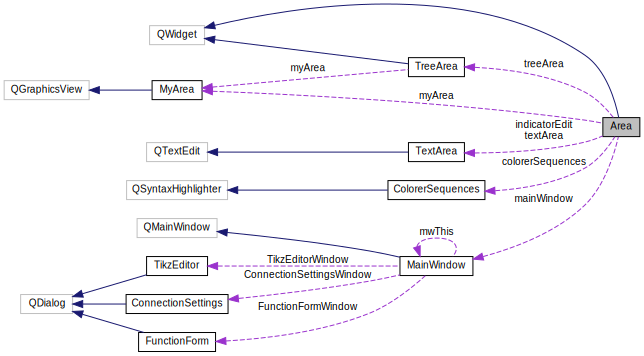
\includegraphics[width=350pt]{classArea__coll__graph}
\end{center}
\end{figure}
\subsection*{Public Slots}
\begin{DoxyCompactItemize}
\item 
\hypertarget{classArea_a36014f76da996d4d3177fab5af44b42d}{void \hyperlink{classArea_a36014f76da996d4d3177fab5af44b42d}{hide\+Or\+Show\+Text} ()}\label{classArea_a36014f76da996d4d3177fab5af44b42d}

\begin{DoxyCompactList}\small\item\em method to hide or show the text area clicking on the button \end{DoxyCompactList}\item 
\hypertarget{classArea_a124912e5857e74fe14f65b15330a493b}{void \hyperlink{classArea_a124912e5857e74fe14f65b15330a493b}{expand\+Or\+Reduce\+Text} ()}\label{classArea_a124912e5857e74fe14f65b15330a493b}

\begin{DoxyCompactList}\small\item\em method to expand or reduce the text area clicking on the button \end{DoxyCompactList}\item 
\hypertarget{classArea_a2972e1d905e8e118d51903e4fccb3648}{void \hyperlink{classArea_a2972e1d905e8e118d51903e4fccb3648}{hide\+Or\+Show\+Tree} ()}\label{classArea_a2972e1d905e8e118d51903e4fccb3648}

\begin{DoxyCompactList}\small\item\em method to hide or show the text area clicking on the button \end{DoxyCompactList}\item 
\hypertarget{classArea_afbffb8cb88542aa9b70e1ef5fb00f47a}{void \hyperlink{classArea_afbffb8cb88542aa9b70e1ef5fb00f47a}{cancel\+Edit} ()}\label{classArea_afbffb8cb88542aa9b70e1ef5fb00f47a}

\begin{DoxyCompactList}\small\item\em method to cancel text change clicking on the button \end{DoxyCompactList}\item 
\hypertarget{classArea_a2f682bc0956a716b4997dd0c82111246}{void \hyperlink{classArea_a2f682bc0956a716b4997dd0c82111246}{save\+Edit} (int del=0)}\label{classArea_a2f682bc0956a716b4997dd0c82111246}

\begin{DoxyCompactList}\small\item\em method to save text change clicking on the button \end{DoxyCompactList}\item 
\hypertarget{classArea_a40389ebbbb18a08cfe7f8257af8600d1}{void \hyperlink{classArea_a40389ebbbb18a08cfe7f8257af8600d1}{on\+Text\+Edit} ()}\label{classArea_a40389ebbbb18a08cfe7f8257af8600d1}

\begin{DoxyCompactList}\small\item\em method call by the signal text\+Changed() \end{DoxyCompactList}\item 
\hypertarget{classArea_abd44d8064b461f85abfd74263b69fb20}{void \hyperlink{classArea_abd44d8064b461f85abfd74263b69fb20}{set\+Old\+Text} ()}\label{classArea_abd44d8064b461f85abfd74263b69fb20}

\begin{DoxyCompactList}\small\item\em method to save all the new text\+Area into the Q\+String\+List \end{DoxyCompactList}\item 
\hypertarget{classArea_add92db2a542dbd1d6e3611834615eb09}{void \hyperlink{classArea_add92db2a542dbd1d6e3611834615eb09}{show\+Tool\+Tip} ()}\label{classArea_add92db2a542dbd1d6e3611834615eb09}

\begin{DoxyCompactList}\small\item\em method to show the tooltip about shortcuts of Q\+Text\+Edit \end{DoxyCompactList}\item 
\hypertarget{classArea_a66b28b7643058f05c36dcd9ea7717b36}{void \hyperlink{classArea_a66b28b7643058f05c36dcd9ea7717b36}{hide\+Tool\+Tip} ()}\label{classArea_a66b28b7643058f05c36dcd9ea7717b36}

\begin{DoxyCompactList}\small\item\em method to hide the tooltip about shortcuts of Q\+Text\+Edit \end{DoxyCompactList}\item 
\hypertarget{classArea_a9dfe0c8071d54a82eb9f5d0d939e4e82}{void \hyperlink{classArea_a9dfe0c8071d54a82eb9f5d0d939e4e82}{temp\+X\+M\+Lfile} ()}\label{classArea_a9dfe0c8071d54a82eb9f5d0d939e4e82}

\begin{DoxyCompactList}\small\item\em method to make the X\+M\+L temporary file before edition \end{DoxyCompactList}\item 
\hypertarget{classArea_a8d72a6b4b6a641627078599805ac675e}{void \hyperlink{classArea_a8d72a6b4b6a641627078599805ac675e}{delete\+Temp\+X\+M\+L} ()}\label{classArea_a8d72a6b4b6a641627078599805ac675e}

\begin{DoxyCompactList}\small\item\em method to delete the X\+M\+L temporary file after update \end{DoxyCompactList}\end{DoxyCompactItemize}
\subsection*{Signals}
\begin{DoxyCompactItemize}
\item 
\hypertarget{classArea_a1e7dcab3e158c58d22d4f5096336b784}{void \hyperlink{classArea_a1e7dcab3e158c58d22d4f5096336b784}{edition} ()}\label{classArea_a1e7dcab3e158c58d22d4f5096336b784}

\begin{DoxyCompactList}\small\item\em Indicate edition. \end{DoxyCompactList}\item 
\hypertarget{classArea_af1d326edb69ae3b42235b93ed664c691}{void \hyperlink{classArea_af1d326edb69ae3b42235b93ed664c691}{make\+Temp\+X\+M\+L} ()}\label{classArea_af1d326edb69ae3b42235b93ed664c691}

\begin{DoxyCompactList}\small\item\em Moment when the X\+M\+L temporary file has to be write. \end{DoxyCompactList}\end{DoxyCompactItemize}
\subsection*{Public Member Functions}
\begin{DoxyCompactItemize}
\item 
\hyperlink{classArea_a6b4b4faf9f541b9071af669c59b49dd9}{Area} (Q\+Widget $\ast$parent=0, Q\+String=\char`\"{}\char`\"{})
\begin{DoxyCompactList}\small\item\em constructor for \hyperlink{classArea}{Area} \end{DoxyCompactList}\item 
\hypertarget{classArea_a93e6b5cec522625ca0ad121fb60c9319}{void \hyperlink{classArea_a93e6b5cec522625ca0ad121fb60c9319}{hide\+Text} ()}\label{classArea_a93e6b5cec522625ca0ad121fb60c9319}

\begin{DoxyCompactList}\small\item\em hides the text. Called from a signal in \hyperlink{classMainWindow}{Main\+Window} \end{DoxyCompactList}\item 
\hypertarget{classArea_a8d4dedd9261bd7299801221b71f6405e}{void \hyperlink{classArea_a8d4dedd9261bd7299801221b71f6405e}{show\+Text} ()}\label{classArea_a8d4dedd9261bd7299801221b71f6405e}

\begin{DoxyCompactList}\small\item\em shows the text. Called from a signal in \hyperlink{classMainWindow}{Main\+Window} \end{DoxyCompactList}\item 
\hypertarget{classArea_ad2d39f0bdbe63a3df0e93baab91139a2}{void \hyperlink{classArea_ad2d39f0bdbe63a3df0e93baab91139a2}{hide\+Tree} ()}\label{classArea_ad2d39f0bdbe63a3df0e93baab91139a2}

\begin{DoxyCompactList}\small\item\em hides the text. Called from a signal in \hyperlink{classMainWindow}{Main\+Window} \end{DoxyCompactList}\item 
\hypertarget{classArea_a536387c9433a7587d4dd23afc3ec2ebd}{void \hyperlink{classArea_a536387c9433a7587d4dd23afc3ec2ebd}{show\+Tree} ()}\label{classArea_a536387c9433a7587d4dd23afc3ec2ebd}

\begin{DoxyCompactList}\small\item\em shows the text. Called from a signal in \hyperlink{classMainWindow}{Main\+Window} \end{DoxyCompactList}\item 
\hypertarget{classArea_a101856bd6a6716144d468130db4a34d6}{void \hyperlink{classArea_a101856bd6a6716144d468130db4a34d6}{edit\+Text} ()}\label{classArea_a101856bd6a6716144d468130db4a34d6}

\begin{DoxyCompactList}\small\item\em Temporary save of the text\+Area called by the signal of right\+Button. \end{DoxyCompactList}\item 
\hypertarget{classArea_aa1091e597fb4957f7fa930e79f286205}{Q\+File \hyperlink{classArea_aa1091e597fb4957f7fa930e79f286205}{get\+Temp\+X\+M\+L} ()}\label{classArea_aa1091e597fb4957f7fa930e79f286205}

\begin{DoxyCompactList}\small\item\em Return the temporary file for automatic import/export. \end{DoxyCompactList}\end{DoxyCompactItemize}
\subsection*{Public Attributes}
\begin{DoxyCompactItemize}
\item 
\hypertarget{classArea_a34549bb32869fc241c911f2c8f6e6344}{Q\+String \hyperlink{classArea_a34549bb32869fc241c911f2c8f6e6344}{path}}\label{classArea_a34549bb32869fc241c911f2c8f6e6344}

\begin{DoxyCompactList}\small\item\em pointer to the path \end{DoxyCompactList}\item 
\hypertarget{classArea_a5f8c84227f46d0584f64d9026e7e3917}{Q\+String \hyperlink{classArea_a5f8c84227f46d0584f64d9026e7e3917}{old\+Text}}\label{classArea_a5f8c84227f46d0584f64d9026e7e3917}

\begin{DoxyCompactList}\small\item\em Text before edition. \end{DoxyCompactList}\item 
\hypertarget{classArea_a3c00ea9bb14425efbee3fcf80410c4cf}{\hyperlink{classMyArea}{My\+Area} $\ast$ \hyperlink{classArea_a3c00ea9bb14425efbee3fcf80410c4cf}{my\+Area}}\label{classArea_a3c00ea9bb14425efbee3fcf80410c4cf}

\begin{DoxyCompactList}\small\item\em pointer to the \hyperlink{classMyArea}{My\+Area} \end{DoxyCompactList}\item 
\hypertarget{classArea_a330747ed9932e54f1fb3c5a8089149b9}{\hyperlink{classTextArea}{Text\+Area} $\ast$ \hyperlink{classArea_a330747ed9932e54f1fb3c5a8089149b9}{indicator\+Edit}}\label{classArea_a330747ed9932e54f1fb3c5a8089149b9}

\begin{DoxyCompactList}\small\item\em pointer to the indicator\+Edit \end{DoxyCompactList}\item 
\hypertarget{classArea_a001e5b841c3e4126a128de13171f05d3}{\hyperlink{classTextArea}{Text\+Area} $\ast$ \hyperlink{classArea_a001e5b841c3e4126a128de13171f05d3}{text\+Area}}\label{classArea_a001e5b841c3e4126a128de13171f05d3}

\begin{DoxyCompactList}\small\item\em pointer to the \hyperlink{classTextArea}{Text\+Area}; \end{DoxyCompactList}\item 
\hypertarget{classArea_a950b6ed9a4e754ef1a7879b727ea8749}{\hyperlink{classTreeArea}{Tree\+Area} $\ast$ \hyperlink{classArea_a950b6ed9a4e754ef1a7879b727ea8749}{tree\+Area}}\label{classArea_a950b6ed9a4e754ef1a7879b727ea8749}

\begin{DoxyCompactList}\small\item\em pointer to the tree\+Area; \end{DoxyCompactList}\item 
\hypertarget{classArea_a78dfb0c8316dbe90af1e5c905db5b6d1}{\hyperlink{classMainWindow}{Main\+Window} $\ast$ \hyperlink{classArea_a78dfb0c8316dbe90af1e5c905db5b6d1}{main\+Window}}\label{classArea_a78dfb0c8316dbe90af1e5c905db5b6d1}

\begin{DoxyCompactList}\small\item\em pointer to the \hyperlink{classMainWindow}{Main\+Window}; \end{DoxyCompactList}\item 
\hypertarget{classArea_a6c88fecf579e816309421ebb2f4110e8}{Q\+Widget $\ast$ \hyperlink{classArea_a6c88fecf579e816309421ebb2f4110e8}{text\+Button\+Area}}\label{classArea_a6c88fecf579e816309421ebb2f4110e8}

\begin{DoxyCompactList}\small\item\em pointer to the widget containing the hide / show text buttons \end{DoxyCompactList}\item 
\hypertarget{classArea_a48df84597b567dfc8b54305ca9faf072}{Q\+Widget $\ast$ \hyperlink{classArea_a48df84597b567dfc8b54305ca9faf072}{tree\+Button\+Area}}\label{classArea_a48df84597b567dfc8b54305ca9faf072}

\begin{DoxyCompactList}\small\item\em pointer to the widget containing the hide / show tree button \end{DoxyCompactList}\item 
\hypertarget{classArea_ac3abf6be3202aedd2cc9ccf8da053989}{Q\+Push\+Button $\ast$ \hyperlink{classArea_ac3abf6be3202aedd2cc9ccf8da053989}{left\+Button}}\label{classArea_ac3abf6be3202aedd2cc9ccf8da053989}

\begin{DoxyCompactList}\small\item\em pointer to the hide / show tree button \end{DoxyCompactList}\item 
\hypertarget{classArea_a7dda00e73b5dda5bcf308bc9451d47aa}{Q\+Push\+Button $\ast$ \hyperlink{classArea_a7dda00e73b5dda5bcf308bc9451d47aa}{right\+Button}}\label{classArea_a7dda00e73b5dda5bcf308bc9451d47aa}

\begin{DoxyCompactList}\small\item\em pointer to the hide / show text button \end{DoxyCompactList}\item 
\hypertarget{classArea_abe2c125e65ad35f1a154ec4b044a7cf1}{Q\+Push\+Button $\ast$ \hyperlink{classArea_abe2c125e65ad35f1a154ec4b044a7cf1}{right\+Expand\+Button}}\label{classArea_abe2c125e65ad35f1a154ec4b044a7cf1}

\begin{DoxyCompactList}\small\item\em pointer to the expand / reduce text button \end{DoxyCompactList}\item 
\hypertarget{classArea_a9f02653780f96daba713c2e71e562da6}{Q\+Push\+Button $\ast$ \hyperlink{classArea_a9f02653780f96daba713c2e71e562da6}{save\+Text\+Edit}}\label{classArea_a9f02653780f96daba713c2e71e562da6}

\begin{DoxyCompactList}\small\item\em pointer to save edit text button \end{DoxyCompactList}\item 
\hypertarget{classArea_a48b08ee11ec952b793e8d92dfc9ef7d4}{Q\+Push\+Button $\ast$ \hyperlink{classArea_a48b08ee11ec952b793e8d92dfc9ef7d4}{cancel\+Text\+Edit}}\label{classArea_a48b08ee11ec952b793e8d92dfc9ef7d4}

\begin{DoxyCompactList}\small\item\em pointer to cancel edit text button \end{DoxyCompactList}\item 
\hypertarget{classArea_a5dde170cf27046b457c18a7f05b78a51}{\hyperlink{classColorerSequences}{Colorer\+Sequences} $\ast$ \hyperlink{classArea_a5dde170cf27046b457c18a7f05b78a51}{colorer\+Sequences}}\label{classArea_a5dde170cf27046b457c18a7f05b78a51}

\begin{DoxyCompactList}\small\item\em pointer to color text in the text\+Area \end{DoxyCompactList}\item 
\hypertarget{classArea_a631ca23eb7e0c5d256239fae64768c1c}{Q\+String\+List $\ast$ \hyperlink{classArea_a631ca23eb7e0c5d256239fae64768c1c}{list\+Old\+Text}}\label{classArea_a631ca23eb7e0c5d256239fae64768c1c}

\begin{DoxyCompactList}\small\item\em Q\+String\+List containing all the text change. \end{DoxyCompactList}\item 
\hypertarget{classArea_a130f9f82732c15bbc56208da9cd1c6d8}{int \hyperlink{classArea_a130f9f82732c15bbc56208da9cd1c6d8}{type\+Of\+Cancel}}\label{classArea_a130f9f82732c15bbc56208da9cd1c6d8}

\begin{DoxyCompactList}\small\item\em int indicating the moment when the user click on Cancel ( 1 \+: after update, 0 \+: during edition ) \end{DoxyCompactList}\end{DoxyCompactItemize}


\subsection{Detailed Description}
New Tab extends Q\+Widget. 

Definition at line 16 of file Area.\+h.



\subsection{Constructor \& Destructor Documentation}
\hypertarget{classArea_a6b4b4faf9f541b9071af669c59b49dd9}{\index{Area@{Area}!Area@{Area}}
\index{Area@{Area}!Area@{Area}}
\subsubsection[{Area}]{\setlength{\rightskip}{0pt plus 5cm}Area\+::\+Area (
\begin{DoxyParamCaption}
\item[{Q\+Widget $\ast$}]{parent = {\ttfamily 0}, }
\item[{Q\+String}]{path = {\ttfamily \char`\"{}\char`\"{}}}
\end{DoxyParamCaption}
)}}\label{classArea_a6b4b4faf9f541b9071af669c59b49dd9}


constructor for \hyperlink{classArea}{Area} 


\begin{DoxyParams}{Parameters}
{\em Q\+Widget} & parent, the widget containing the \hyperlink{classArea}{Area}, which is the Tabbed\+View \\
\hline
\end{DoxyParams}


Definition at line 7 of file Area.\+cpp.


\begin{DoxyCode}
7                                         :
8     QWidget(parent) \{
9     this->\hyperlink{classArea_a34549bb32869fc241c911f2c8f6e6344}{path} = \hyperlink{classArea_a34549bb32869fc241c911f2c8f6e6344}{path};
10 
11     \textcolor{comment}{// call the constructors of all the areas}
12     this->\hyperlink{classArea_a001e5b841c3e4126a128de13171f05d3}{textArea} = \textcolor{keyword}{new} \hyperlink{classTextArea}{TextArea}(\textcolor{keyword}{this});
13     this->\hyperlink{classArea_a001e5b841c3e4126a128de13171f05d3}{textArea}->setReadOnly(\textcolor{keyword}{false});
14     this->\hyperlink{classArea_a3c00ea9bb14425efbee3fcf80410c4cf}{myArea} = \textcolor{keyword}{new} \hyperlink{classMyArea}{MyArea}(\textcolor{keyword}{this}, this->\hyperlink{classArea_a34549bb32869fc241c911f2c8f6e6344}{path});
15     this->\hyperlink{classArea_a950b6ed9a4e754ef1a7879b727ea8749}{treeArea} = \textcolor{keyword}{new} \hyperlink{classTreeArea}{TreeArea}(\textcolor{keyword}{this});
16     this->\hyperlink{classArea_a330747ed9932e54f1fb3c5a8089149b9}{indicatorEdit} = \textcolor{keyword}{new} \hyperlink{classTextArea}{TextArea}(\textcolor{keyword}{this});
17     this->\hyperlink{classArea_a631ca23eb7e0c5d256239fae64768c1c}{listOldText} = \textcolor{keyword}{new} QStringList();
18 
19     \textcolor{comment}{//Add text coloration (lie le TextArea)}
20     \hyperlink{classArea_a5dde170cf27046b457c18a7f05b78a51}{colorerSequences} = \textcolor{keyword}{new} \hyperlink{classColorerSequences}{ColorerSequences}(
      \hyperlink{classArea_a001e5b841c3e4126a128de13171f05d3}{textArea}->document());
21 
22     \textcolor{comment}{// treeArea: create widgets containing the buttons}
23     this->\hyperlink{classArea_a48df84597b567dfc8b54305ca9faf072}{treeButtonArea} = \textcolor{keyword}{new} QWidget(\textcolor{keyword}{this});
24     this->treeButtonArea->setMinimumWidth(12);
25     this->treeButtonArea->setMaximumWidth(12);
26     this->\hyperlink{classArea_a6c88fecf579e816309421ebb2f4110e8}{textButtonArea} = \textcolor{keyword}{new} QWidget(\textcolor{keyword}{this});
27     this->\hyperlink{classArea_a6c88fecf579e816309421ebb2f4110e8}{textButtonArea}->setMinimumWidth(12);
28     this->\hyperlink{classArea_a6c88fecf579e816309421ebb2f4110e8}{textButtonArea}->setMaximumWidth(12);
29 
30     \textcolor{comment}{// create the buttons}
31     this->\hyperlink{classArea_ac3abf6be3202aedd2cc9ccf8da053989}{leftButton} = \textcolor{keyword}{new} QPushButton(\textcolor{stringliteral}{"<"}, this->treeButtonArea);
32     this->\hyperlink{classArea_ac3abf6be3202aedd2cc9ccf8da053989}{leftButton}->setMaximumWidth(12);
33     this->\hyperlink{classArea_ac3abf6be3202aedd2cc9ccf8da053989}{leftButton}->setMinimumHeight(70);
34     QVBoxLayout *layoutLeft = \textcolor{keyword}{new} QVBoxLayout;
35     layoutLeft->addWidget(\hyperlink{classArea_ac3abf6be3202aedd2cc9ccf8da053989}{leftButton});
36     layoutLeft->setContentsMargins(0,0,0,0);
37     this->treeButtonArea->setLayout(layoutLeft);
38 
39     this->\hyperlink{classArea_a7dda00e73b5dda5bcf308bc9451d47aa}{rightButton} = \textcolor{keyword}{new} QPushButton(\textcolor{stringliteral}{">"}, this->\hyperlink{classArea_a6c88fecf579e816309421ebb2f4110e8}{textButtonArea});
40     this->\hyperlink{classArea_a7dda00e73b5dda5bcf308bc9451d47aa}{rightButton}->setMaximumWidth(12);
41     this->\hyperlink{classArea_a7dda00e73b5dda5bcf308bc9451d47aa}{rightButton}->setMinimumHeight(70);
42     this->\hyperlink{classArea_abe2c125e65ad35f1a154ec4b044a7cf1}{rightExpandButton} = \textcolor{keyword}{new} QPushButton(\textcolor{stringliteral}{"<"}, this->
      \hyperlink{classArea_a6c88fecf579e816309421ebb2f4110e8}{textButtonArea});
43     this->\hyperlink{classArea_abe2c125e65ad35f1a154ec4b044a7cf1}{rightExpandButton}->setMaximumWidth(12);
44     this->\hyperlink{classArea_abe2c125e65ad35f1a154ec4b044a7cf1}{rightExpandButton}->setMinimumHeight(70);
45     QVBoxLayout *layoutRight = \textcolor{keyword}{new} QVBoxLayout;
46     layoutRight->addWidget(this->\hyperlink{classArea_a7dda00e73b5dda5bcf308bc9451d47aa}{rightButton});
47     layoutRight->addWidget(this->\hyperlink{classArea_abe2c125e65ad35f1a154ec4b044a7cf1}{rightExpandButton});
48     layoutRight->setContentsMargins(0,0,0,0);
49     this->\hyperlink{classArea_a6c88fecf579e816309421ebb2f4110e8}{textButtonArea}->setLayout(layoutRight);
50 
51     this->\hyperlink{classArea_a9f02653780f96daba713c2e71e562da6}{saveTextEdit} = \textcolor{keyword}{new} QPushButton(\textcolor{stringliteral}{"Update"},\textcolor{keyword}{this});
52     this->\hyperlink{classArea_a9f02653780f96daba713c2e71e562da6}{saveTextEdit}->setFixedSize(QSize(80,30));
53     this->\hyperlink{classArea_a9f02653780f96daba713c2e71e562da6}{saveTextEdit}->setVisible(\textcolor{keyword}{false});
54     this->\hyperlink{classArea_a9f02653780f96daba713c2e71e562da6}{saveTextEdit}->setEnabled(\textcolor{keyword}{false});
55     this->\hyperlink{classArea_a9f02653780f96daba713c2e71e562da6}{saveTextEdit}->setShortcut(QKeySequence((Qt::CTRL + Qt::Key\_E)));
56 
57     this->\hyperlink{classArea_a48b08ee11ec952b793e8d92dfc9ef7d4}{cancelTextEdit} = \textcolor{keyword}{new} QPushButton(\textcolor{stringliteral}{"Cancel"},\textcolor{keyword}{this});
58     this->\hyperlink{classArea_a48b08ee11ec952b793e8d92dfc9ef7d4}{cancelTextEdit}->setFixedSize(QSize(80,30));
59     this->\hyperlink{classArea_a48b08ee11ec952b793e8d92dfc9ef7d4}{cancelTextEdit}->setVisible(\textcolor{keyword}{false});
60     this->\hyperlink{classArea_a48b08ee11ec952b793e8d92dfc9ef7d4}{cancelTextEdit}->setEnabled(\textcolor{keyword}{false});
61 
62     \textcolor{comment}{//indicatorEdit preferences}
63 
64     this->\hyperlink{classArea_a330747ed9932e54f1fb3c5a8089149b9}{indicatorEdit}->setReadOnly(\textcolor{keyword}{true});
65     this->\hyperlink{classArea_a330747ed9932e54f1fb3c5a8089149b9}{indicatorEdit}->\hyperlink{classTextArea_acdfa220612113b805f8653dce6b7624e}{changeBackgroundColor}(QColor(\textcolor{stringliteral}{"#F1F1F1"}));
66     this->\hyperlink{classArea_a330747ed9932e54f1fb3c5a8089149b9}{indicatorEdit}->setFixedSize(QSize(200,27));
67     this->\hyperlink{classArea_a330747ed9932e54f1fb3c5a8089149b9}{indicatorEdit}->setTextColor(QColor(228,26,4));
68     this->\hyperlink{classArea_a330747ed9932e54f1fb3c5a8089149b9}{indicatorEdit}->setCurrentFont(QFont(\textcolor{stringliteral}{"TypeWriter"},10));
69     this->\hyperlink{classArea_a330747ed9932e54f1fb3c5a8089149b9}{indicatorEdit}->setFontWeight(5);
70     this->\hyperlink{classArea_a330747ed9932e54f1fb3c5a8089149b9}{indicatorEdit}->setFrameShape(QTextEdit::NoFrame);
71     this->\hyperlink{classArea_a330747ed9932e54f1fb3c5a8089149b9}{indicatorEdit}->setFrameShadow(QTextEdit::Plain);
72     this->\hyperlink{classArea_a330747ed9932e54f1fb3c5a8089149b9}{indicatorEdit}->setPlainText(\textcolor{stringliteral}{"Edition..."});
73     this->\hyperlink{classArea_a330747ed9932e54f1fb3c5a8089149b9}{indicatorEdit}->setVisible(\textcolor{keyword}{false});
74     \textcolor{comment}{//Press CTRL+E to save or CTRL+ESC to cancel}
75 
76     \textcolor{comment}{// set the global layout}
77     QHBoxLayout *layout = \textcolor{keyword}{new} QHBoxLayout;
78     layout->addWidget(this->\hyperlink{classArea_a950b6ed9a4e754ef1a7879b727ea8749}{treeArea});
79     layout->addWidget(this->treeButtonArea);
80     layout->addWidget(this->\hyperlink{classArea_a3c00ea9bb14425efbee3fcf80410c4cf}{myArea});
81     layout->addWidget(this->\hyperlink{classArea_a6c88fecf579e816309421ebb2f4110e8}{textButtonArea});
82 
83     QVBoxLayout *VLayout = \textcolor{keyword}{new} QVBoxLayout;
84     VLayout->addWidget(this->\hyperlink{classArea_a330747ed9932e54f1fb3c5a8089149b9}{indicatorEdit});
85     VLayout->addWidget(this->\hyperlink{classArea_a001e5b841c3e4126a128de13171f05d3}{textArea});
86 
87     QHBoxLayout *options = \textcolor{keyword}{new} QHBoxLayout;
88     options->addWidget(this->\hyperlink{classArea_a9f02653780f96daba713c2e71e562da6}{saveTextEdit});
89     options->addWidget(this->\hyperlink{classArea_a48b08ee11ec952b793e8d92dfc9ef7d4}{cancelTextEdit});
90 
91     VLayout->addLayout(options);
92 
93     QHBoxLayout *global = \textcolor{keyword}{new} QHBoxLayout;
94     global->addLayout(layout);
95     global->addLayout(VLayout);
96 
97     this->setLayout(global);
98 
99     \textcolor{comment}{// connect}
100     QObject::connect(this->\hyperlink{classArea_ac3abf6be3202aedd2cc9ccf8da053989}{leftButton}, SIGNAL(clicked()), \textcolor{keyword}{this}, SLOT(
      \hyperlink{classArea_a2972e1d905e8e118d51903e4fccb3648}{hideOrShowTree}()));
101     QObject::connect(this->\hyperlink{classArea_a7dda00e73b5dda5bcf308bc9451d47aa}{rightButton}, SIGNAL(clicked()), \textcolor{keyword}{this}, SLOT(
      \hyperlink{classArea_a36014f76da996d4d3177fab5af44b42d}{hideOrShowText}()));
102     QObject::connect(this->\hyperlink{classArea_abe2c125e65ad35f1a154ec4b044a7cf1}{rightExpandButton}, SIGNAL(clicked()), \textcolor{keyword}{this}, SLOT(
      \hyperlink{classArea_a124912e5857e74fe14f65b15330a493b}{expandOrReduceText}()));
103     QObject::connect(this->\hyperlink{classArea_a48b08ee11ec952b793e8d92dfc9ef7d4}{cancelTextEdit}, SIGNAL(clicked()), \textcolor{keyword}{this}, SLOT(
      \hyperlink{classArea_afbffb8cb88542aa9b70e1ef5fb00f47a}{cancelEdit}()));
104     QObject::connect(this->\hyperlink{classArea_a001e5b841c3e4126a128de13171f05d3}{textArea}, SIGNAL(textChanged()), this->
      \hyperlink{classArea_a001e5b841c3e4126a128de13171f05d3}{textArea}, SLOT(\hyperlink{classArea_a40389ebbbb18a08cfe7f8257af8600d1}{onTextEdit}()));
105     QObject::connect(this->\hyperlink{classArea_a9f02653780f96daba713c2e71e562da6}{saveTextEdit}, SIGNAL(clicked()), \textcolor{keyword}{this}, SLOT(
      \hyperlink{classArea_a2f682bc0956a716b4997dd0c82111246}{saveEdit}()));
106     QObject::connect(this->\hyperlink{classArea_a001e5b841c3e4126a128de13171f05d3}{textArea}, SIGNAL(textChanged()), \textcolor{keyword}{this}, SLOT(
      \hyperlink{classArea_a40389ebbbb18a08cfe7f8257af8600d1}{onTextEdit}()));
107     QObject::connect(\textcolor{keyword}{this}, SIGNAL(\hyperlink{classArea_a1e7dcab3e158c58d22d4f5096336b784}{edition}()), \textcolor{keyword}{this}, SLOT(\hyperlink{classArea_add92db2a542dbd1d6e3611834615eb09}{showToolTip}()));
108     QObject::connect(\textcolor{keyword}{this}, SIGNAL(\hyperlink{classArea_af1d326edb69ae3b42235b93ed664c691}{makeTempXML}()), \textcolor{keyword}{this}, SLOT(
      \hyperlink{classArea_a9dfe0c8071d54a82eb9f5d0d939e4e82}{tempXMLfile}()));
109 
110     \textcolor{comment}{// initialization}
111     this->\hyperlink{classArea_a001e5b841c3e4126a128de13171f05d3}{textArea}->setHidden(\textcolor{keyword}{true});
112     this->\hyperlink{classArea_a7dda00e73b5dda5bcf308bc9451d47aa}{rightButton}->setText(\textcolor{stringliteral}{"<"});
113     this->\hyperlink{classArea_abe2c125e65ad35f1a154ec4b044a7cf1}{rightExpandButton}->hide();
114     this->\hyperlink{classArea_a9f02653780f96daba713c2e71e562da6}{saveTextEdit}->setDefault(\textcolor{keyword}{false});
115     this->\hyperlink{classArea_a48b08ee11ec952b793e8d92dfc9ef7d4}{cancelTextEdit}->setDefault(\textcolor{keyword}{false});
116 \}
\end{DoxyCode}


The documentation for this class was generated from the following files\+:\begin{DoxyCompactItemize}
\item 
headers/Area.\+h\item 
src/ui/Area.\+cpp\end{DoxyCompactItemize}

\hypertarget{classArgumentFrame}{\section{Argument\+Frame Class Reference}
\label{classArgumentFrame}\index{Argument\+Frame@{Argument\+Frame}}
}
\subsection*{Public Member Functions}
\begin{DoxyCompactItemize}
\item 
\hypertarget{classArgumentFrame_a078f53c29943421581053f45eef1138a}{Q\+String {\bfseries get\+Arg\+Number} ()}\label{classArgumentFrame_a078f53c29943421581053f45eef1138a}

\item 
\hypertarget{classArgumentFrame_af18e760bf2a9d9c1c663742fd378cf89}{void {\bfseries set\+Arg\+Number} (Q\+String new\+Arg\+Number)}\label{classArgumentFrame_af18e760bf2a9d9c1c663742fd378cf89}

\item 
\hypertarget{classArgumentFrame_aa3f6b9a043f92570c01fc63bc2ec082c}{Q\+String {\bfseries get\+Arg\+Suf} ()}\label{classArgumentFrame_aa3f6b9a043f92570c01fc63bc2ec082c}

\item 
\hypertarget{classArgumentFrame_afc8b164e67cb7eab93cf6e85b847176f}{void {\bfseries set\+Arg\+Suf} (Q\+String new\+Arg\+Suf)}\label{classArgumentFrame_afc8b164e67cb7eab93cf6e85b847176f}

\item 
\hypertarget{classArgumentFrame_a7490cff5cada50746f9f5aab061ac396}{Q\+String {\bfseries get\+Arg\+Type} ()}\label{classArgumentFrame_a7490cff5cada50746f9f5aab061ac396}

\item 
\hypertarget{classArgumentFrame_a2d18e376c85b15296108ddb3135052a1}{void {\bfseries set\+Arg\+Type} (Q\+String new\+Arg\+Type)}\label{classArgumentFrame_a2d18e376c85b15296108ddb3135052a1}

\item 
\hypertarget{classArgumentFrame_aab5a56938a83beecedf1c0e8a4cd04fe}{Q\+String {\bfseries get\+Arg\+Fac} ()}\label{classArgumentFrame_aab5a56938a83beecedf1c0e8a4cd04fe}

\item 
\hypertarget{classArgumentFrame_ac0f0e26ee22afe6b091c67e4c23c5657}{void {\bfseries set\+Arg\+Fac} (Q\+String new\+Arg\+Fac)}\label{classArgumentFrame_ac0f0e26ee22afe6b091c67e4c23c5657}

\item 
\hypertarget{classArgumentFrame_a4c298cd5165a191b2ad1a75c96994c32}{Q\+String {\bfseries get\+Arg\+Outline} ()}\label{classArgumentFrame_a4c298cd5165a191b2ad1a75c96994c32}

\item 
\hypertarget{classArgumentFrame_a73f63181a96c7c67ac3452b792359292}{void {\bfseries set\+Arg\+Outline} (Q\+String new\+Arg\+Outline)}\label{classArgumentFrame_a73f63181a96c7c67ac3452b792359292}

\end{DoxyCompactItemize}


\subsection{Detailed Description}


Definition at line 6 of file Argument\+Frame.\+h.



The documentation for this class was generated from the following files\+:\begin{DoxyCompactItemize}
\item 
headers/Argument\+Frame.\+h\item 
src/ui/Argument\+Frame.\+cpp\end{DoxyCompactItemize}

\hypertarget{classChoixLigne}{\section{Choix\+Ligne Class Reference}
\label{classChoixLigne}\index{Choix\+Ligne@{Choix\+Ligne}}
}
\subsection*{Public Member Functions}
\begin{DoxyCompactItemize}
\item 
\hypertarget{classChoixLigne_abdf282f67694452f4381f025b97c7bca}{Q\+String {\bfseries get\+Choix\+Nom} ()}\label{classChoixLigne_abdf282f67694452f4381f025b97c7bca}

\item 
\hypertarget{classChoixLigne_a29c424c6c3b527ac5ed1c6b037255238}{void {\bfseries set\+Choix\+Nom} (Q\+String new\+Choix\+Nom)}\label{classChoixLigne_a29c424c6c3b527ac5ed1c6b037255238}

\item 
\hypertarget{classChoixLigne_af07e6270bd35ba0d47232df004e1959e}{Q\+String {\bfseries get\+Choix\+Param} ()}\label{classChoixLigne_af07e6270bd35ba0d47232df004e1959e}

\item 
\hypertarget{classChoixLigne_a16a376319258f72bb4d72c49f6af073e}{void {\bfseries set\+Choix\+Param} (Q\+String new\+Choix\+Param)}\label{classChoixLigne_a16a376319258f72bb4d72c49f6af073e}

\item 
\hypertarget{classChoixLigne_a7e3802f6cd05adb6b77a71eb7a265e38}{Q\+String {\bfseries get\+Choix\+Prefix} ()}\label{classChoixLigne_a7e3802f6cd05adb6b77a71eb7a265e38}

\item 
\hypertarget{classChoixLigne_adece79d84d7e2b92fb2f8bbfb5abab33}{void {\bfseries set\+Choix\+Prefix} (Q\+String new\+Choix\+Prefix)}\label{classChoixLigne_adece79d84d7e2b92fb2f8bbfb5abab33}

\end{DoxyCompactItemize}


\subsection{Detailed Description}


Definition at line 6 of file Choix\+Ligne.\+h.



The documentation for this class was generated from the following files\+:\begin{DoxyCompactItemize}
\item 
headers/test/Choix\+Ligne.\+h\item 
src/ui/Choix\+Ligne.\+cpp\end{DoxyCompactItemize}

\hypertarget{classColorerSequences}{\section{Colorer\+Sequences Class Reference}
\label{classColorerSequences}\index{Colorer\+Sequences@{Colorer\+Sequences}}
}


Inheritance diagram for Colorer\+Sequences\+:\nopagebreak
\begin{figure}[H]
\begin{center}
\leavevmode
\includegraphics[width=181pt]{classColorerSequences__inherit__graph}
\end{center}
\end{figure}


Collaboration diagram for Colorer\+Sequences\+:\nopagebreak
\begin{figure}[H]
\begin{center}
\leavevmode
\includegraphics[width=181pt]{classColorerSequences__coll__graph}
\end{center}
\end{figure}
\subsection*{Public Slots}
\begin{DoxyCompactItemize}
\item 
\hypertarget{classColorerSequences_a33fa40a05a61f1a9448c8c16fc07f0b4}{void {\bfseries highlight\+Block} (const Q\+String \&text)}\label{classColorerSequences_a33fa40a05a61f1a9448c8c16fc07f0b4}

\end{DoxyCompactItemize}
\subsection*{Public Member Functions}
\begin{DoxyCompactItemize}
\item 
\hypertarget{classColorerSequences_a370adf65a6762bfc723652040cf7f20b}{{\bfseries Colorer\+Sequences} (Q\+Text\+Document $\ast$parent=0)}\label{classColorerSequences_a370adf65a6762bfc723652040cf7f20b}

\end{DoxyCompactItemize}
\subsection*{Public Attributes}
\begin{DoxyCompactItemize}
\item 
\hypertarget{classColorerSequences_a8e7ab751ba21c01472e778c35dc4693a}{std\+::vector$<$ Q\+Text\+Char\+Format $>$ {\bfseries tab\+Class\+Format}}\label{classColorerSequences_a8e7ab751ba21c01472e778c35dc4693a}

\item 
\hypertarget{classColorerSequences_aa034ff8b9f1bf525ed71ba3ebb6c998f}{std\+::vector$<$ Q\+String $>$ {\bfseries tab\+Pattern}}\label{classColorerSequences_aa034ff8b9f1bf525ed71ba3ebb6c998f}

\item 
\hypertarget{classColorerSequences_ad3acffb41c936ed6acb3e8ceba2ecd6e}{std\+::vector$<$ Q\+Reg\+Exp $>$ {\bfseries tab\+Expression}}\label{classColorerSequences_ad3acffb41c936ed6acb3e8ceba2ecd6e}

\item 
\hypertarget{classColorerSequences_aa04308f7ecf022f7c025c7e6f3985b45}{std\+::vector$<$ int $>$ {\bfseries tab\+Index}}\label{classColorerSequences_aa04308f7ecf022f7c025c7e6f3985b45}

\end{DoxyCompactItemize}


\subsection{Detailed Description}


Definition at line 7 of file Colorer\+Sequences.\+h.



The documentation for this class was generated from the following files\+:\begin{DoxyCompactItemize}
\item 
headers/Colorer\+Sequences.\+h\item 
src/ui/Colorer\+Sequences.\+cpp\end{DoxyCompactItemize}

\hypertarget{classConnectionSettings}{\section{Connection\+Settings Class Reference}
\label{classConnectionSettings}\index{Connection\+Settings@{Connection\+Settings}}
}


Inheritance diagram for Connection\+Settings\+:\nopagebreak
\begin{figure}[H]
\begin{center}
\leavevmode
\includegraphics[width=182pt]{classConnectionSettings__inherit__graph}
\end{center}
\end{figure}


Collaboration diagram for Connection\+Settings\+:\nopagebreak
\begin{figure}[H]
\begin{center}
\leavevmode
\includegraphics[width=182pt]{classConnectionSettings__coll__graph}
\end{center}
\end{figure}
\subsection*{Static Public Member Functions}
\begin{DoxyCompactItemize}
\item 
\hypertarget{classConnectionSettings_a6a2336ec802e7759fe6ed7ed8a4e736b}{static void {\bfseries import\+X\+M\+L\+Settings} ()}\label{classConnectionSettings_a6a2336ec802e7759fe6ed7ed8a4e736b}

\end{DoxyCompactItemize}
\subsection*{Public Attributes}
\begin{DoxyCompactItemize}
\item 
\hypertarget{classConnectionSettings_a255f866adcca66025ae71d8fff01f708}{std\+::vector$<$ Q\+Label $\ast$ $>$ {\bfseries tab\+Arg\+Number}}\label{classConnectionSettings_a255f866adcca66025ae71d8fff01f708}

\item 
\hypertarget{classConnectionSettings_acabf7a26c24257ceb58a20e2faedc1d7}{std\+::vector$<$ Q\+Combo\+Box $\ast$ $>$ {\bfseries tab\+Arg\+Type}}\label{classConnectionSettings_acabf7a26c24257ceb58a20e2faedc1d7}

\item 
\hypertarget{classConnectionSettings_aaa24d0415cbe3cea62e9e223b85e4b1e}{std\+::vector$<$ Q\+String $>$ {\bfseries tab\+Arg\+Type\+Mem}}\label{classConnectionSettings_aaa24d0415cbe3cea62e9e223b85e4b1e}

\item 
\hypertarget{classConnectionSettings_a4d1c136cb1b682352e729be9df56f476}{std\+::vector$<$ Q\+Widget $\ast$ $>$ {\bfseries tab\+Arg\+Suf}}\label{classConnectionSettings_a4d1c136cb1b682352e729be9df56f476}

\item 
\hypertarget{classConnectionSettings_afc80dd0a61bb1a80ded2abda3d11a634}{std\+::vector$<$ Q\+Check\+Box $\ast$ $>$ {\bfseries tab\+Argfacul}}\label{classConnectionSettings_afc80dd0a61bb1a80ded2abda3d11a634}

\item 
\hypertarget{classConnectionSettings_a782c02d6ba749aaf1b30fb44135bcc69}{std\+::vector$<$ Q\+Line\+Edit $\ast$ $>$ {\bfseries tab\+Arg\+Outline}}\label{classConnectionSettings_a782c02d6ba749aaf1b30fb44135bcc69}

\item 
\hypertarget{classConnectionSettings_a7aecc71eb4a2560579e204591a22a56f}{std\+::vector$<$ Q\+Line\+Edit $\ast$ $>$ {\bfseries tab\+Tampon}}\label{classConnectionSettings_a7aecc71eb4a2560579e204591a22a56f}

\item 
\hypertarget{classConnectionSettings_a60c6c6b6d298134bf26ad06e0fb6377c}{std\+::vector$<$ Q\+Line\+Edit $\ast$ $>$ {\bfseries tab\+Tampon\+Param}}\label{classConnectionSettings_a60c6c6b6d298134bf26ad06e0fb6377c}

\item 
\hypertarget{classConnectionSettings_a07dd3a760944aa5c0df4fc70ec152fd9}{std\+::vector$<$ Q\+Line\+Edit $\ast$ $>$ {\bfseries tab\+Tampon\+Prefix}}\label{classConnectionSettings_a07dd3a760944aa5c0df4fc70ec152fd9}

\item 
\hypertarget{classConnectionSettings_a066cb9704304701e0c87b48002761a56}{std\+::vector$<$ Q\+Line\+Edit $\ast$ $>$ {\bfseries tab\+Choix\+Nom}}\label{classConnectionSettings_a066cb9704304701e0c87b48002761a56}

\item 
\hypertarget{classConnectionSettings_ae95584bcca066a6ccc154ea1158588ac}{std\+::vector$<$ Q\+Line\+Edit $\ast$ $>$ {\bfseries tab\+Choix\+Param}}\label{classConnectionSettings_ae95584bcca066a6ccc154ea1158588ac}

\item 
\hypertarget{classConnectionSettings_a3a6e0f2946dd56bd2c8d9b08a569760c}{std\+::vector$<$ Q\+Line\+Edit $\ast$ $>$ {\bfseries tab\+Choix\+Prefix}}\label{classConnectionSettings_a3a6e0f2946dd56bd2c8d9b08a569760c}

\item 
\hypertarget{classConnectionSettings_a8a046e7e52ea721a4af8eb99123e4bb7}{int {\bfseries nb\+Arg\+Prcdt}}\label{classConnectionSettings_a8a046e7e52ea721a4af8eb99123e4bb7}

\item 
\hypertarget{classConnectionSettings_a8dbd9f61f430a8ad42f8ac6dd85384a7}{int {\bfseries row\+Max}}\label{classConnectionSettings_a8dbd9f61f430a8ad42f8ac6dd85384a7}

\item 
\hypertarget{classConnectionSettings_ac71a066165c1dc84a2a13277ef84f7a1}{std\+::vector$<$ Q\+String $>$ {\bfseries tab\+Choix\+Prcdt}}\label{classConnectionSettings_ac71a066165c1dc84a2a13277ef84f7a1}

\end{DoxyCompactItemize}
\subsection*{Static Public Attributes}
\begin{DoxyCompactItemize}
\item 
\hypertarget{classConnectionSettings_ae84807deffb7c52220cca228d29b18ff}{static std\+::vector$<$ \hyperlink{classFuncFrame}{Func\+Frame} $\ast$ $>$ {\bfseries tab\+Function}}\label{classConnectionSettings_ae84807deffb7c52220cca228d29b18ff}

\item 
\hypertarget{classConnectionSettings_a439ae757f9ef6cd2a035ac9eae0721b5}{static std\+::vector\\*
$<$ std\+::vector$<$ \hyperlink{classArgumentFrame}{Argument\+Frame} $\ast$ $>$ $\ast$ $>$ {\bfseries tab\+Argument}}\label{classConnectionSettings_a439ae757f9ef6cd2a035ac9eae0721b5}

\item 
\hypertarget{classConnectionSettings_af5b6db02baab00f652f609ddef48a771}{static std\+::vector\\*
$<$ std\+::vector$<$ std\+::vector\\*
$<$ \hyperlink{classChoixLigne}{Choix\+Ligne} $\ast$ $>$ $\ast$ $>$ $\ast$ $>$ {\bfseries tab\+Choix}}\label{classConnectionSettings_af5b6db02baab00f652f609ddef48a771}

\item 
\hypertarget{classConnectionSettings_afe95edc3c1946bd9bd600bd53519e4cd}{static Q\+String\+List {\bfseries arg\+Type\+List}}\label{classConnectionSettings_afe95edc3c1946bd9bd600bd53519e4cd}

\end{DoxyCompactItemize}


\subsection{Detailed Description}


Definition at line 13 of file Connection\+Settings.\+h.



The documentation for this class was generated from the following files\+:\begin{DoxyCompactItemize}
\item 
headers/Connection\+Settings.\+h\item 
src/ui/Connection\+Settings.\+cpp\item 
src/ui/Function\+Form.\+cpp\end{DoxyCompactItemize}

\hypertarget{structexception__base}{\section{exception\+\_\+base Class Reference}
\label{structexception__base}\index{exception\+\_\+base@{exception\+\_\+base}}
}


struct defining the base of the exception  




{\ttfamily \#include $<$Exceptions.\+h$>$}



Inheritance diagram for exception\+\_\+base\+:\nopagebreak
\begin{figure}[H]
\begin{center}
\leavevmode
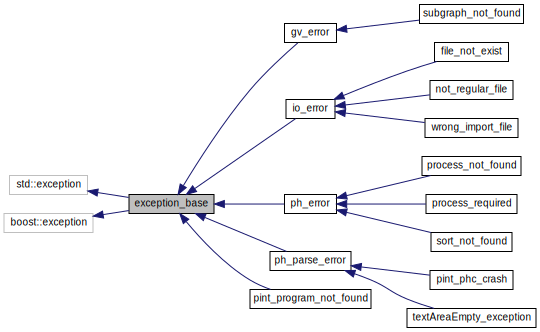
\includegraphics[width=350pt]{structexception__base__inherit__graph}
\end{center}
\end{figure}


Collaboration diagram for exception\+\_\+base\+:\nopagebreak
\begin{figure}[H]
\begin{center}
\leavevmode
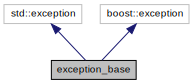
\includegraphics[width=266pt]{structexception__base__coll__graph}
\end{center}
\end{figure}


\subsection{Detailed Description}
struct defining the base of the exception 

Definition at line 20 of file Exceptions.\+h.



The documentation for this class was generated from the following file\+:\begin{DoxyCompactItemize}
\item 
headers/\hyperlink{Exceptions_8h}{Exceptions.\+h}\end{DoxyCompactItemize}

\hypertarget{structfile__not__exist}{\section{file\+\_\+not\+\_\+exist Class Reference}
\label{structfile__not__exist}\index{file\+\_\+not\+\_\+exist@{file\+\_\+not\+\_\+exist}}
}


struct defining the exception called when the file does not exist extends \hyperlink{structio__error}{io\+\_\+error}  




{\ttfamily \#include $<$Exceptions.\+h$>$}



Inheritance diagram for file\+\_\+not\+\_\+exist\+:\nopagebreak
\begin{figure}[H]
\begin{center}
\leavevmode
\includegraphics[width=266pt]{structfile__not__exist__inherit__graph}
\end{center}
\end{figure}


Collaboration diagram for file\+\_\+not\+\_\+exist\+:\nopagebreak
\begin{figure}[H]
\begin{center}
\leavevmode
\includegraphics[width=266pt]{structfile__not__exist__coll__graph}
\end{center}
\end{figure}


\subsection{Detailed Description}
struct defining the exception called when the file does not exist extends \hyperlink{structio__error}{io\+\_\+error} 

Definition at line 38 of file Exceptions.\+h.



The documentation for this class was generated from the following file\+:\begin{DoxyCompactItemize}
\item 
headers/\hyperlink{Exceptions_8h}{Exceptions.\+h}\end{DoxyCompactItemize}

\hypertarget{classFuncFrame}{\section{Func\+Frame Class Reference}
\label{classFuncFrame}\index{Func\+Frame@{Func\+Frame}}
}
\subsection*{Public Member Functions}
\begin{DoxyCompactItemize}
\item 
\hypertarget{classFuncFrame_a916578977ef70ff3c7ee122b6f6db66e}{Q\+String {\bfseries get\+Name\+Function} ()}\label{classFuncFrame_a916578977ef70ff3c7ee122b6f6db66e}

\item 
\hypertarget{classFuncFrame_a5f4f491f860fc85ae9a869dcd38903e9}{void {\bfseries set\+Name\+Function} (Q\+String new\+Name\+Function)}\label{classFuncFrame_a5f4f491f860fc85ae9a869dcd38903e9}

\item 
\hypertarget{classFuncFrame_a88602664b8f523253fd2101e69b37eee}{Q\+String {\bfseries get\+Program} ()}\label{classFuncFrame_a88602664b8f523253fd2101e69b37eee}

\item 
\hypertarget{classFuncFrame_a97f31b356169a11a0d59a7ffae691fc7}{void {\bfseries set\+Program} (Q\+String new\+Program)}\label{classFuncFrame_a97f31b356169a11a0d59a7ffae691fc7}

\item 
\hypertarget{classFuncFrame_a68840fd54f2898a079480b5b2944b01f}{Q\+String {\bfseries get\+Nb\+Argument} ()}\label{classFuncFrame_a68840fd54f2898a079480b5b2944b01f}

\item 
\hypertarget{classFuncFrame_a328e3c73c5a974dc1f6f2e63a89a640a}{void {\bfseries set\+Nb\+Argument} (Q\+String new\+Nb\+Argument)}\label{classFuncFrame_a328e3c73c5a974dc1f6f2e63a89a640a}

\end{DoxyCompactItemize}


\subsection{Detailed Description}


Definition at line 7 of file Func\+Frame.\+h.



The documentation for this class was generated from the following files\+:\begin{DoxyCompactItemize}
\item 
headers/Func\+Frame.\+h\item 
src/ui/Func\+Frame.\+cpp\end{DoxyCompactItemize}

\hypertarget{classFunctionForm}{\section{Function\+Form Class Reference}
\label{classFunctionForm}\index{Function\+Form@{Function\+Form}}
}


Inheritance diagram for Function\+Form\+:\nopagebreak
\begin{figure}[H]
\begin{center}
\leavevmode
\includegraphics[width=157pt]{classFunctionForm__inherit__graph}
\end{center}
\end{figure}


Collaboration diagram for Function\+Form\+:\nopagebreak
\begin{figure}[H]
\begin{center}
\leavevmode
\includegraphics[width=157pt]{classFunctionForm__coll__graph}
\end{center}
\end{figure}
\subsection*{Public Member Functions}
\begin{DoxyCompactItemize}
\item 
\hypertarget{classFunctionForm_ab2be919d4b96f31dc85d8e133dd9bda0}{{\bfseries Function\+Form} (Q\+String file\+Name)}\label{classFunctionForm_ab2be919d4b96f31dc85d8e133dd9bda0}

\end{DoxyCompactItemize}


\subsection{Detailed Description}


Definition at line 6 of file Function\+Form.\+h.



The documentation for this class was generated from the following files\+:\begin{DoxyCompactItemize}
\item 
headers/Function\+Form.\+h\item 
src/ui/Function\+Form.\+cpp\end{DoxyCompactItemize}

\hypertarget{classGAction}{\section{G\+Action Class Reference}
\label{classGAction}\index{G\+Action@{G\+Action}}
}


contains style and layout info to draw an action  




{\ttfamily \#include $<$G\+Action.\+h$>$}



Collaboration diagram for G\+Action\+:\nopagebreak
\begin{figure}[H]
\begin{center}
\leavevmode
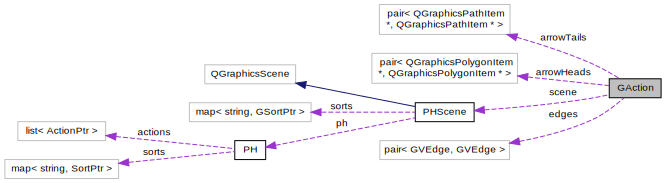
\includegraphics[width=350pt]{classGAction__coll__graph}
\end{center}
\end{figure}
\subsection*{Public Member Functions}
\begin{DoxyCompactItemize}
\item 
\hyperlink{classGAction_a697f4b533d191139a1eb401c486afff9}{G\+Action} (Action\+Ptr a, \hyperlink{structGVEdge}{G\+V\+Edge} e, \hyperlink{structGVEdge}{G\+V\+Edge} f, \hyperlink{classPHScene}{P\+H\+Scene} $\ast$sc)
\begin{DoxyCompactList}\small\item\em constructor \end{DoxyCompactList}\item 
\hyperlink{classGAction_a2e56eb084652d002e5284985c70ebe3d}{G\+Action} (Action\+Ptr a, \hyperlink{classPHScene}{P\+H\+Scene} $\ast$sc)
\begin{DoxyCompactList}\small\item\em constructor \end{DoxyCompactList}\item 
\hypertarget{classGAction_a394daac6bc228e8105790f4493b32387}{void \hyperlink{classGAction_a394daac6bc228e8105790f4493b32387}{update} ()}\label{classGAction_a394daac6bc228e8105790f4493b32387}

\begin{DoxyCompactList}\small\item\em update position of \hyperlink{classGAction}{G\+Action} \end{DoxyCompactList}\item 
Q\+Graphics\+Item $\ast$ \hyperlink{classGAction_a5092e3c2bbdd70a63c914766c0142672}{get\+Display\+Item} (void)
\begin{DoxyCompactList}\small\item\em gets the display \end{DoxyCompactList}\item 
\hypertarget{classGAction_ac9005fd701c1362eea9d7299b95672cb}{Action\+Ptr \hyperlink{classGAction_ac9005fd701c1362eea9d7299b95672cb}{get\+Action} ()}\label{classGAction_ac9005fd701c1362eea9d7299b95672cb}

\begin{DoxyCompactList}\small\item\em gets the action \end{DoxyCompactList}\item 
G\+Process\+Ptr \hyperlink{classGAction_a4f4c104269fd0d40a61b22458db42dee}{get\+Source} ()
\begin{DoxyCompactList}\small\item\em gets the source \hyperlink{classGProcess}{G\+Process} item \end{DoxyCompactList}\item 
G\+Process\+Ptr \hyperlink{classGAction_ac7aff6bc03be3791a8a20a914aae5b2c}{get\+Target} ()
\begin{DoxyCompactList}\small\item\em gets the target \hyperlink{classGProcess}{G\+Process} item \end{DoxyCompactList}\item 
G\+Process\+Ptr \hyperlink{classGAction_ae1ed003118c8333c6afa2e8d30e3dc07}{get\+Result} ()
\begin{DoxyCompactList}\small\item\em gets the result \hyperlink{classGProcess}{G\+Process} item \end{DoxyCompactList}\item 
\hypertarget{classGAction_a29954530df3ca052ba3c7ad5f56de9b3}{bool \hyperlink{classGAction_a29954530df3ca052ba3c7ad5f56de9b3}{is\+Bold} ()}\label{classGAction_a29954530df3ca052ba3c7ad5f56de9b3}

\begin{DoxyCompactList}\small\item\em indicates whether or not this action is in bold \end{DoxyCompactList}\item 
\hypertarget{classGAction_ac50e5adaea34a8e9b358907c32f58f6a}{void \hyperlink{classGAction_ac50e5adaea34a8e9b358907c32f58f6a}{to\+Bold} ()}\label{classGAction_ac50e5adaea34a8e9b358907c32f58f6a}

\begin{DoxyCompactList}\small\item\em change this \hyperlink{classGAction}{G\+Action} to bold \end{DoxyCompactList}\item 
\hypertarget{classGAction_ac6834abb04c34cefed63cb0515e6a712}{void \hyperlink{classGAction_ac6834abb04c34cefed63cb0515e6a712}{color\+Action} (Q\+Color)}\label{classGAction_ac6834abb04c34cefed63cb0515e6a712}

\begin{DoxyCompactList}\small\item\em change this \hyperlink{classGAction}{G\+Action} color \end{DoxyCompactList}\item 
\hypertarget{classGAction_ade1234868fc1ba2b4c5ee1ff7c3ae998}{int \hyperlink{classGAction_ade1234868fc1ba2b4c5ee1ff7c3ae998}{get\+Action\+Color\+Number} ()}\label{classGAction_ade1234868fc1ba2b4c5ee1ff7c3ae998}

\begin{DoxyCompactList}\small\item\em gets the number of color R\+G\+B to tik\+Z file \end{DoxyCompactList}\item 
\hypertarget{classGAction_adfc489f6845c5e9ffa9d361984f5993a}{void \hyperlink{classGAction_adfc489f6845c5e9ffa9d361984f5993a}{set\+Action\+Color\+N\+Umber} (int r, int g, int b, int nb)}\label{classGAction_adfc489f6845c5e9ffa9d361984f5993a}

\begin{DoxyCompactList}\small\item\em sets the number of the process color R\+G\+B to Tik\+Z file \end{DoxyCompactList}\end{DoxyCompactItemize}
\subsection*{Protected Member Functions}
\begin{DoxyCompactItemize}
\item 
\hypertarget{classGAction_a6509f55dc693f00abfc5d019ea244c89}{void \hyperlink{classGAction_a6509f55dc693f00abfc5d019ea244c89}{init\+Contact\+Points} ()}\label{classGAction_a6509f55dc693f00abfc5d019ea244c89}

\begin{DoxyCompactList}\small\item\em init the position of source\+Point\+Line, target\+Point\+Line and result\+Point\+Line \end{DoxyCompactList}\item 
\hypertarget{classGAction_ac3772b10309aa6afe0e64ba40c662fcc}{void \hyperlink{classGAction_ac3772b10309aa6afe0e64ba40c662fcc}{update\+Contact\+Points} ()}\label{classGAction_ac3772b10309aa6afe0e64ba40c662fcc}

\begin{DoxyCompactList}\small\item\em update the position of source\+Point\+Line, target\+Point\+Line and result\+Point\+Line \end{DoxyCompactList}\item 
Q\+Painter\+Path \hyperlink{classGAction_a86dc08d16a482755317f4c212a853068}{create\+Hit\+Path} ()
\begin{DoxyCompactList}\small\item\em build the line corresponding to the first part of the action \end{DoxyCompactList}\item 
Q\+Painter\+Path \hyperlink{classGAction_a682f47e5009ea5336579928215bc6391}{create\+Bound\+Path} ()
\begin{DoxyCompactList}\small\item\em build the arc corresponding to the second part of the action \end{DoxyCompactList}\item 
Q\+Polygon\+F \hyperlink{classGAction_a7144bb80f0de787a60d43340c8545163}{make\+Arrow\+Head} (Q\+Painter\+Path path)
\begin{DoxyCompactList}\small\item\em draws the head of the arrow \end{DoxyCompactList}\item 
\hypertarget{classGAction_a7aa759b10fae92f3052b8d5336641a03}{void \hyperlink{classGAction_a7aa759b10fae92f3052b8d5336641a03}{init\+Points\+In\+Simple\+Modele} ()}\label{classGAction_a7aa759b10fae92f3052b8d5336641a03}

\begin{DoxyCompactList}\small\item\em init contact points to display the \hyperlink{classGAction}{G\+Action} in simple model \end{DoxyCompactList}\item 
\hypertarget{classGAction_a374e74c397d09f202c05e506413a885d}{void \hyperlink{classGAction_a374e74c397d09f202c05e506413a885d}{init\+Points\+In\+Detailled\+Model} ()}\label{classGAction_a374e74c397d09f202c05e506413a885d}

\begin{DoxyCompactList}\small\item\em init contact points to display the \hyperlink{classGAction}{G\+Action} in detailled model \end{DoxyCompactList}\item 
\hypertarget{classGAction_afd02cc0b1d7efcaf012dd9045c22f659}{void \hyperlink{classGAction_afd02cc0b1d7efcaf012dd9045c22f659}{update\+Points\+In\+Simple\+Model} ()}\label{classGAction_afd02cc0b1d7efcaf012dd9045c22f659}

\begin{DoxyCompactList}\small\item\em update contact points to display the \hyperlink{classGAction}{G\+Action} in simple model \end{DoxyCompactList}\item 
\hypertarget{classGAction_af512e122e9c332aa70e804cab303efca}{void \hyperlink{classGAction_af512e122e9c332aa70e804cab303efca}{update\+Points\+In\+Detailled\+Model} ()}\label{classGAction_af512e122e9c332aa70e804cab303efca}

\begin{DoxyCompactList}\small\item\em update contact points to display the \hyperlink{classGAction}{G\+Action} in detailled model \end{DoxyCompactList}\item 
\hypertarget{classGAction_aa03acf91fcd0c6b8eaa4fb5e610e83e5}{bool \hyperlink{classGAction_aa03acf91fcd0c6b8eaa4fb5e610e83e5}{is\+Auto\+Hit} ()}\label{classGAction_aa03acf91fcd0c6b8eaa4fb5e610e83e5}

\begin{DoxyCompactList}\small\item\em check if the source and the target process are the same \end{DoxyCompactList}\item 
\hypertarget{classGAction_a5eb7f465ca07cb553c8d628aae1b125b}{void \hyperlink{classGAction_a5eb7f465ca07cb553c8d628aae1b125b}{init\+Points\+Normal\+Hit} ()}\label{classGAction_a5eb7f465ca07cb553c8d628aae1b125b}

\begin{DoxyCompactList}\small\item\em init contact points in the case of normal hit \end{DoxyCompactList}\item 
\hypertarget{classGAction_a0df07896e15cc7d479d158a28c350713}{void \hyperlink{classGAction_a0df07896e15cc7d479d158a28c350713}{update\+Points\+Normal\+Hit} ()}\label{classGAction_a0df07896e15cc7d479d158a28c350713}

\begin{DoxyCompactList}\small\item\em update contact points in the case of normal hit \end{DoxyCompactList}\item 
\hypertarget{classGAction_a31e9d06194e01e691e1ca8e1a64ad73f}{void \hyperlink{classGAction_a31e9d06194e01e691e1ca8e1a64ad73f}{init\+Points\+Auto\+Hit} ()}\label{classGAction_a31e9d06194e01e691e1ca8e1a64ad73f}

\begin{DoxyCompactList}\small\item\em init contact points in the case of an auto hit \end{DoxyCompactList}\item 
\hypertarget{classGAction_a63727f6b50a489bc6d820055bd040adb}{void \hyperlink{classGAction_a63727f6b50a489bc6d820055bd040adb}{update\+Points\+Auto\+Hit} ()}\label{classGAction_a63727f6b50a489bc6d820055bd040adb}

\begin{DoxyCompactList}\small\item\em init contact points in the case of an auto hit \end{DoxyCompactList}\item 
\hypertarget{classGAction_a92cac7175b3969a54197d401c13f5273}{bool \hyperlink{classGAction_a92cac7175b3969a54197d401c13f5273}{is\+Curved\+Hit} (G\+Sort\+Ptr source\+Sort, G\+Sort\+Ptr target\+Sort, G\+Process\+Ptr source, G\+Process\+Ptr target)}\label{classGAction_a92cac7175b3969a54197d401c13f5273}

\begin{DoxyCompactList}\small\item\em check if the hit needs to be curved \end{DoxyCompactList}\end{DoxyCompactItemize}
\subsection*{Protected Attributes}
\begin{DoxyCompactItemize}
\item 
\hypertarget{classGAction_a5318deb6935859f5d2ebd1836ec6eb85}{\hyperlink{classPHScene}{P\+H\+Scene} $\ast$ \hyperlink{classGAction_a5318deb6935859f5d2ebd1836ec6eb85}{scene}}\label{classGAction_a5318deb6935859f5d2ebd1836ec6eb85}

\begin{DoxyCompactList}\small\item\em the \hyperlink{classPHScene}{P\+H\+Scene} related to the \hyperlink{classAction}{Action} \end{DoxyCompactList}\item 
\hypertarget{classGAction_a80fd22faf283374dd9861bf4900eafa4}{Q\+Graphics\+Item $\ast$ \hyperlink{classGAction_a80fd22faf283374dd9861bf4900eafa4}{display}}\label{classGAction_a80fd22faf283374dd9861bf4900eafa4}

\begin{DoxyCompactList}\small\item\em the graphical item representing the \hyperlink{classAction}{Action} \end{DoxyCompactList}\item 
\hypertarget{classGAction_a7d9568fcba3679f9ff9edc71beee92f5}{Q\+Graphics\+Path\+Item $\ast$ \hyperlink{classGAction_a7d9568fcba3679f9ff9edc71beee92f5}{hit\+Line}}\label{classGAction_a7d9568fcba3679f9ff9edc71beee92f5}

\begin{DoxyCompactList}\small\item\em line representing the first part of the action \end{DoxyCompactList}\item 
\hypertarget{classGAction_a2ff47768398033e52bd3b78586b1d29c}{Q\+Graphics\+Path\+Item $\ast$ \hyperlink{classGAction_a2ff47768398033e52bd3b78586b1d29c}{bound\+Arc}}\label{classGAction_a2ff47768398033e52bd3b78586b1d29c}

\begin{DoxyCompactList}\small\item\em path representing the second part of the action \end{DoxyCompactList}\item 
\hypertarget{classGAction_ad6992ac8b540932c370f5b46c48bbe70}{Q\+Point\+F $\ast$ \hyperlink{classGAction_ad6992ac8b540932c370f5b46c48bbe70}{target\+Point}}\label{classGAction_ad6992ac8b540932c370f5b46c48bbe70}

\begin{DoxyCompactList}\small\item\em target Point of the line representing the first part of the action \end{DoxyCompactList}\item 
\hypertarget{classGAction_adf67bcd561238d7626566cebeee2a151}{Q\+Point\+F $\ast$ \hyperlink{classGAction_adf67bcd561238d7626566cebeee2a151}{source\+Point}}\label{classGAction_adf67bcd561238d7626566cebeee2a151}

\begin{DoxyCompactList}\small\item\em source Point of the line representing the first part of the action \end{DoxyCompactList}\item 
\hypertarget{classGAction_a08d6b4a2f2d04a46861dafbe38897d8a}{Q\+Point\+F $\ast$ \hyperlink{classGAction_a08d6b4a2f2d04a46861dafbe38897d8a}{result\+Point}}\label{classGAction_a08d6b4a2f2d04a46861dafbe38897d8a}

\begin{DoxyCompactList}\small\item\em source Point of the arc representing the second part of the action \end{DoxyCompactList}\item 
\hypertarget{classGAction_a22f734f6fb2fade298681819341b4f75}{Action\+Ptr \hyperlink{classGAction_a22f734f6fb2fade298681819341b4f75}{action}}\label{classGAction_a22f734f6fb2fade298681819341b4f75}

\begin{DoxyCompactList}\small\item\em the related \hyperlink{classAction}{Action} \end{DoxyCompactList}\item 
\hypertarget{classGAction_a806d5854710a68e9d59a0b035628f7a4}{bool \hyperlink{classGAction_a806d5854710a68e9d59a0b035628f7a4}{bold}}\label{classGAction_a806d5854710a68e9d59a0b035628f7a4}

\begin{DoxyCompactList}\small\item\em if the action is in bold or not \end{DoxyCompactList}\item 
int \hyperlink{classGAction_aaa7f90de74ad249e8c0054728d1339d1}{number\+Action\+Color}
\begin{DoxyCompactList}\small\item\em the pair of graphical items representing the tails of the arrows of the \hyperlink{classAction}{Action} \end{DoxyCompactList}\item 
\hypertarget{classGAction_abc626fc7dc52a5f02960706c02a52db9}{pair$<$ Q\+Graphics\+Path\+Item \\*
$\ast$, Q\+Graphics\+Path\+Item $\ast$ $>$ {\bfseries arrow\+Tails}}\label{classGAction_abc626fc7dc52a5f02960706c02a52db9}

\item 
\hypertarget{classGAction_aab9cc72a8692e0b15f19e192ab21d609}{pair$<$ Q\+Graphics\+Polygon\+Item \\*
$\ast$, Q\+Graphics\+Polygon\+Item $\ast$ $>$ \hyperlink{classGAction_aab9cc72a8692e0b15f19e192ab21d609}{arrow\+Heads}}\label{classGAction_aab9cc72a8692e0b15f19e192ab21d609}

\begin{DoxyCompactList}\small\item\em the pair of graphical items representing the heads of the arrows of the \hyperlink{classAction}{Action} \end{DoxyCompactList}\item 
\hypertarget{classGAction_a65f9f4938e024adc07cea387079549f8}{pair$<$ \hyperlink{structGVEdge}{G\+V\+Edge}, \hyperlink{structGVEdge}{G\+V\+Edge} $>$ \hyperlink{classGAction_a65f9f4938e024adc07cea387079549f8}{edges}}\label{classGAction_a65f9f4938e024adc07cea387079549f8}

\begin{DoxyCompactList}\small\item\em the edges related to the arrows \end{DoxyCompactList}\end{DoxyCompactItemize}


\subsection{Detailed Description}
contains style and layout info to draw an action 

Definition at line 38 of file G\+Action.\+h.



\subsection{Constructor \& Destructor Documentation}
\hypertarget{classGAction_a697f4b533d191139a1eb401c486afff9}{\index{G\+Action@{G\+Action}!G\+Action@{G\+Action}}
\index{G\+Action@{G\+Action}!G\+Action@{G\+Action}}
\subsubsection[{G\+Action}]{\setlength{\rightskip}{0pt plus 5cm}G\+Action\+::\+G\+Action (
\begin{DoxyParamCaption}
\item[{Action\+Ptr}]{a, }
\item[{{\bf G\+V\+Edge}}]{e, }
\item[{{\bf G\+V\+Edge}}]{f, }
\item[{{\bf P\+H\+Scene} $\ast$}]{sc}
\end{DoxyParamCaption}
)}}\label{classGAction_a697f4b533d191139a1eb401c486afff9}


constructor 


\begin{DoxyParams}{Parameters}
{\em Action\+Ptr} & the related \hyperlink{classAction}{Action} object \\
\hline
{\em \hyperlink{structGVEdge}{G\+V\+Edge}} & the object that contains style and layout info for hit arrow \\
\hline
{\em \hyperlink{structGVEdge}{G\+V\+Edge}} & the object that contains style and layout info for bounce (result) arrow \\
\hline
{\em \hyperlink{classPHScene}{P\+H\+Scene}} & the related scene \\
\hline
\end{DoxyParams}
\hypertarget{classGAction_a2e56eb084652d002e5284985c70ebe3d}{\index{G\+Action@{G\+Action}!G\+Action@{G\+Action}}
\index{G\+Action@{G\+Action}!G\+Action@{G\+Action}}
\subsubsection[{G\+Action}]{\setlength{\rightskip}{0pt plus 5cm}G\+Action\+::\+G\+Action (
\begin{DoxyParamCaption}
\item[{Action\+Ptr}]{a, }
\item[{{\bf P\+H\+Scene} $\ast$}]{sc}
\end{DoxyParamCaption}
)}}\label{classGAction_a2e56eb084652d002e5284985c70ebe3d}


constructor 


\begin{DoxyParams}{Parameters}
{\em Action\+Ptr} & the related \hyperlink{classAction}{Action} object \\
\hline
{\em \hyperlink{classPHScene}{P\+H\+Scene}} & the related scene \\
\hline
\end{DoxyParams}


Definition at line 18 of file G\+Action.\+cpp.


\begin{DoxyCode}
18                                          : \hyperlink{classGAction_a5318deb6935859f5d2ebd1836ec6eb85}{scene}(sc), \hyperlink{classGAction_a22f734f6fb2fade298681819341b4f75}{action}(a) \{
19     \hyperlink{classGAction_a80fd22faf283374dd9861bf4900eafa4}{display} = \textcolor{keyword}{new} QGraphicsItemGroup();
20 
21     \hyperlink{classGAction_a6509f55dc693f00abfc5d019ea244c89}{initContactPoints}();
22 
23     \hyperlink{classGAction_a7d9568fcba3679f9ff9edc71beee92f5}{hitLine}= \textcolor{keyword}{new} QGraphicsPathItem(\hyperlink{classGAction_a86dc08d16a482755317f4c212a853068}{createHitPath}(),\hyperlink{classGAction_a80fd22faf283374dd9861bf4900eafa4}{display});
24     \textcolor{keywordflow}{if}((\hyperlink{classGAction_ad6992ac8b540932c370f5b46c48bbe70}{targetPoint}->x()==\hyperlink{classGAction_a08d6b4a2f2d04a46861dafbe38897d8a}{resultPoint}->x())&&(\hyperlink{classGAction_ad6992ac8b540932c370f5b46c48bbe70}{targetPoint}->y()==
      \hyperlink{classGAction_a08d6b4a2f2d04a46861dafbe38897d8a}{resultPoint}->y())) \{
25         QPen pen;
26         pen.setWidth(2);
27         pen.setBrush(Qt::red);
28         \hyperlink{classGAction_a7d9568fcba3679f9ff9edc71beee92f5}{hitLine}->setPen(pen);
29     \} \textcolor{keywordflow}{else} \{
30         QPen pen;
31         pen.setWidth(1);
32         pen.setBrush(Qt::black);
33         \hyperlink{classGAction_a7d9568fcba3679f9ff9edc71beee92f5}{hitLine}->setPen(pen);
34     \}
35 
36     \hyperlink{classGAction_a2ff47768398033e52bd3b78586b1d29c}{boundArc} = \textcolor{keyword}{new} QGraphicsPathItem(\hyperlink{classGAction_a682f47e5009ea5336579928215bc6391}{createBoundPath}(),
      \hyperlink{classGAction_a80fd22faf283374dd9861bf4900eafa4}{display});
37     \hyperlink{classGAction_a2ff47768398033e52bd3b78586b1d29c}{boundArc}->setPen(QPen(Qt::DashLine));
38     \hyperlink{classGAction_aaa7f90de74ad249e8c0054728d1339d1}{numberActionColor}=-1;
39     this->\hyperlink{classGAction_a806d5854710a68e9d59a0b035628f7a4}{bold}=\textcolor{keyword}{false};
40 
41 \}
\end{DoxyCode}


\subsection{Member Function Documentation}
\hypertarget{classGAction_a682f47e5009ea5336579928215bc6391}{\index{G\+Action@{G\+Action}!create\+Bound\+Path@{create\+Bound\+Path}}
\index{create\+Bound\+Path@{create\+Bound\+Path}!G\+Action@{G\+Action}}
\subsubsection[{create\+Bound\+Path}]{\setlength{\rightskip}{0pt plus 5cm}Q\+Painter\+Path G\+Action\+::create\+Bound\+Path (
\begin{DoxyParamCaption}
{}
\end{DoxyParamCaption}
)\hspace{0.3cm}{\ttfamily [protected]}}}\label{classGAction_a682f47e5009ea5336579928215bc6391}


build the arc corresponding to the second part of the action 

\begin{DoxyReturn}{Returns}
Q\+Painter\+Path the arc representing the second part of the action 
\end{DoxyReturn}


Definition at line 361 of file G\+Action.\+cpp.


\begin{DoxyCode}
361                                       \{
362     QPainterPath boundPath(*\hyperlink{classGAction_ad6992ac8b540932c370f5b46c48bbe70}{targetPoint});
363 
364     \textcolor{keywordflow}{if}((\hyperlink{classGAction_ad6992ac8b540932c370f5b46c48bbe70}{targetPoint}->x()!=\hyperlink{classGAction_a08d6b4a2f2d04a46861dafbe38897d8a}{resultPoint}->x())||(\hyperlink{classGAction_ad6992ac8b540932c370f5b46c48bbe70}{targetPoint}->y()!=
      \hyperlink{classGAction_a08d6b4a2f2d04a46861dafbe38897d8a}{resultPoint}->y())) \{
365         qreal rectCornerX;
366         qreal rectCornerY;
367         qreal widthRect;
368         qreal heightRect;
369         qreal sweepAngle;
370         qreal startAngle;
371         \textcolor{keywordtype}{int} invertSweep;
372 
373         \textcolor{keywordflow}{if}(dynamic\_cast<GSort*>(\hyperlink{classGAction_ac7aff6bc03be3791a8a20a914aae5b2c}{getTarget}()->getDisplayItem()->parentItem())->isVertical()) \{
374             \textcolor{keywordflow}{if}(\hyperlink{classGAction_ad6992ac8b540932c370f5b46c48bbe70}{targetPoint}->y()<\hyperlink{classGAction_a08d6b4a2f2d04a46861dafbe38897d8a}{resultPoint}->y()) \{
375                 rectCornerY = \hyperlink{classGAction_ad6992ac8b540932c370f5b46c48bbe70}{targetPoint}->y();
376                 heightRect = \hyperlink{classGAction_a08d6b4a2f2d04a46861dafbe38897d8a}{resultPoint}->y()-\hyperlink{classGAction_ad6992ac8b540932c370f5b46c48bbe70}{targetPoint}->y();
377                 startAngle = 90;
378                 invertSweep = 1;
379             \} \textcolor{keywordflow}{else} \{
380                 rectCornerY = \hyperlink{classGAction_a08d6b4a2f2d04a46861dafbe38897d8a}{resultPoint}->y();
381                 heightRect = \hyperlink{classGAction_ad6992ac8b540932c370f5b46c48bbe70}{targetPoint}->y()-\hyperlink{classGAction_a08d6b4a2f2d04a46861dafbe38897d8a}{resultPoint}->y();
382                 startAngle = -90;
383                 invertSweep = -1;
384             \}
385 
386             \textcolor{keywordflow}{if}(\hyperlink{classGAction_a08d6b4a2f2d04a46861dafbe38897d8a}{resultPoint}->x() < \hyperlink{classGAction_ae1ed003118c8333c6afa2e8d30e3dc07}{getResult}()->getCenterPoint()->x()) \{
387                 sweepAngle = 180*invertSweep;
388             \} \textcolor{keywordflow}{else} \{
389                 sweepAngle = -180*invertSweep;
390             \}
391 
392             rectCornerX = \hyperlink{classGAction_a08d6b4a2f2d04a46861dafbe38897d8a}{resultPoint}->x()- (GProcess::sizeDefault)/2.0;
393             widthRect = GProcess::sizeDefault;
394         \} \textcolor{keywordflow}{else} \{
395 
396             \textcolor{keywordflow}{if}(\hyperlink{classGAction_ad6992ac8b540932c370f5b46c48bbe70}{targetPoint}->x()<\hyperlink{classGAction_a08d6b4a2f2d04a46861dafbe38897d8a}{resultPoint}->x()) \{ \textcolor{comment}{//target point à gauche de
       resultpoint}
397                 rectCornerX = \hyperlink{classGAction_ad6992ac8b540932c370f5b46c48bbe70}{targetPoint}->x();
398                 widthRect = \hyperlink{classGAction_a08d6b4a2f2d04a46861dafbe38897d8a}{resultPoint}->x() - \hyperlink{classGAction_ad6992ac8b540932c370f5b46c48bbe70}{targetPoint}->x();
399                 startAngle =180;
400                 invertSweep = -1;
401             \} \textcolor{keywordflow}{else} \{ \textcolor{comment}{//resultpoint à gauche de targetpoint}
402                 rectCornerX = \hyperlink{classGAction_a08d6b4a2f2d04a46861dafbe38897d8a}{resultPoint}->x();
403                 widthRect = \hyperlink{classGAction_ad6992ac8b540932c370f5b46c48bbe70}{targetPoint}->x() - \hyperlink{classGAction_a08d6b4a2f2d04a46861dafbe38897d8a}{resultPoint}->x();
404                 startAngle =0;
405                 invertSweep = 1;
406             \}
407             \textcolor{keywordflow}{if}(\hyperlink{classGAction_a08d6b4a2f2d04a46861dafbe38897d8a}{resultPoint}->y()<\hyperlink{classGAction_ae1ed003118c8333c6afa2e8d30e3dc07}{getResult}()->getCenterPoint()->y()) \{ \textcolor{comment}{//resultpoint
       au-dessus du centre du process}
408                 rectCornerY = \hyperlink{classGAction_a08d6b4a2f2d04a46861dafbe38897d8a}{resultPoint}->y()-(GProcess::sizeDefault)/2.0;
409                 sweepAngle = 180*invertSweep;
410             \} \textcolor{keywordflow}{else} \{ \textcolor{comment}{//resultpoint en-dessus du centre du process}
411                 rectCornerY= \hyperlink{classGAction_a08d6b4a2f2d04a46861dafbe38897d8a}{resultPoint}->y()-(GProcess::sizeDefault)/2.0;
412                 sweepAngle = -180*invertSweep;
413             \}
414             heightRect = GProcess::sizeDefault;
415         \}
416 
417 
418         boundPath.arcTo(QRectF(rectCornerX,rectCornerY,widthRect,heightRect),startAngle,sweepAngle);
419 
420         boundPath.addPolygon(\hyperlink{classGAction_a7144bb80f0de787a60d43340c8545163}{makeArrowHead}(boundPath));
421     \}
422 
423     \textcolor{keywordflow}{return} boundPath;
424 \}
\end{DoxyCode}
\hypertarget{classGAction_a86dc08d16a482755317f4c212a853068}{\index{G\+Action@{G\+Action}!create\+Hit\+Path@{create\+Hit\+Path}}
\index{create\+Hit\+Path@{create\+Hit\+Path}!G\+Action@{G\+Action}}
\subsubsection[{create\+Hit\+Path}]{\setlength{\rightskip}{0pt plus 5cm}Q\+Painter\+Path G\+Action\+::create\+Hit\+Path (
\begin{DoxyParamCaption}
{}
\end{DoxyParamCaption}
)\hspace{0.3cm}{\ttfamily [protected]}}}\label{classGAction_a86dc08d16a482755317f4c212a853068}


build the line corresponding to the first part of the action 

\begin{DoxyReturn}{Returns}
Q\+Painter\+Path the line representing the first part of the action 
\end{DoxyReturn}
invert\+Start 

Definition at line 265 of file G\+Action.\+cpp.


\begin{DoxyCode}
265                                     \{
266 
267     GProcessPtr source = \hyperlink{classGAction_a4f4c104269fd0d40a61b22458db42dee}{getSource}();
268     GProcessPtr target = \hyperlink{classGAction_ac7aff6bc03be3791a8a20a914aae5b2c}{getTarget}();
269     GProcessPtr result = \hyperlink{classGAction_ae1ed003118c8333c6afa2e8d30e3dc07}{getResult}();
270     GSortPtr sourceSort = \hyperlink{classGAction_a5318deb6935859f5d2ebd1836ec6eb85}{scene}->\hyperlink{classPHScene_ae8be020b063c06f135d644937d65147b}{getGSort}(\hyperlink{classGAction_a22f734f6fb2fade298681819341b4f75}{action}->getSource()->getSort()->getName());
271     GSortPtr targetSort = \hyperlink{classGAction_a5318deb6935859f5d2ebd1836ec6eb85}{scene}->\hyperlink{classPHScene_ae8be020b063c06f135d644937d65147b}{getGSort}(\hyperlink{classGAction_a22f734f6fb2fade298681819341b4f75}{action}->getTarget()->getSort()->getName());
272 
273 
274     qreal rectCornerX;
275     qreal rectCornerY;
276     qreal widthRect;
277     qreal heightRect;
278     qreal sweepAngle;
279     qreal startAngle;
280     \textcolor{keywordtype}{int} invertSweep;
281     \textcolor{keywordtype}{int} invertStart;
282     \textcolor{keywordtype}{int} wCoef=1;
283     \textcolor{keywordtype}{int} hCoef=1;
284 
285     QPointF* controlPointSource;
286     QPointF* controlPointTarget;
287 
288     QLineF* hitLineTemp;
289     hitLineTemp = \textcolor{keyword}{new} QLineF(*\hyperlink{classGAction_adf67bcd561238d7626566cebeee2a151}{sourcePoint},*\hyperlink{classGAction_ad6992ac8b540932c370f5b46c48bbe70}{targetPoint});
290 
291     QPainterPath hitPath(*\hyperlink{classGAction_adf67bcd561238d7626566cebeee2a151}{sourcePoint});
292 
293     \textcolor{keywordflow}{if}(!\hyperlink{classGAction_aa03acf91fcd0c6b8eaa4fb5e610e83e5}{isAutoHit}()) \{
294         \textcolor{keywordflow}{if}(\hyperlink{classGAction_a92cac7175b3969a54197d401c13f5273}{isCurvedHit}(sourceSort, targetSort, source, target) && (sourceSort->getSimpleDisplay(
      )!=1 || targetSort->getSimpleDisplay()!=1)) \{
295             \textcolor{keywordflow}{if}(\hyperlink{classGAction_adf67bcd561238d7626566cebeee2a151}{sourcePoint}->x() >= \hyperlink{classGAction_ad6992ac8b540932c370f5b46c48bbe70}{targetPoint}->x()) \{
296                 wCoef= -1;
297             \} \textcolor{keywordflow}{else} \{
298                 wCoef= 1;
299             \}
300             \textcolor{keywordflow}{if}(\hyperlink{classGAction_adf67bcd561238d7626566cebeee2a151}{sourcePoint}->y() >= \hyperlink{classGAction_ad6992ac8b540932c370f5b46c48bbe70}{targetPoint}->y()) \{
301                 hCoef = 1;
302             \} \textcolor{keywordflow}{else} \{
303                 hCoef = -1;
304             \}
305             controlPointSource = \textcolor{keyword}{new} QPointF(\hyperlink{classGAction_adf67bcd561238d7626566cebeee2a151}{sourcePoint}->x() + wCoef*hitLineTemp->length()/2.0,
      \hyperlink{classGAction_adf67bcd561238d7626566cebeee2a151}{sourcePoint}->y()-hCoef*hitLineTemp->length()/3.0);
306             controlPointTarget = \textcolor{keyword}{new} QPointF(\hyperlink{classGAction_ad6992ac8b540932c370f5b46c48bbe70}{targetPoint}->x() + wCoef*hitLineTemp->length()/2.0,
      \hyperlink{classGAction_ad6992ac8b540932c370f5b46c48bbe70}{targetPoint}->y() + hCoef*hitLineTemp->length()/3.0);
307 
308             hitPath.cubicTo(*controlPointSource,*controlPointTarget, *
      \hyperlink{classGAction_ad6992ac8b540932c370f5b46c48bbe70}{targetPoint});
309         \} \textcolor{keywordflow}{else} \{
310             hitPath.lineTo(*\hyperlink{classGAction_ad6992ac8b540932c370f5b46c48bbe70}{targetPoint});
311         \}
312     \} \textcolor{keywordflow}{else} \textcolor{keywordflow}{if} ( (\hyperlink{classGAction_aa03acf91fcd0c6b8eaa4fb5e610e83e5}{isAutoHit}() && sourceSort->getSimpleDisplay() != 1)
313                 ||targetSort->getSimpleDisplay()!=1) \{
314         \textcolor{keywordflow}{if}(dynamic\_cast<GSort*>(\hyperlink{classGAction_ac7aff6bc03be3791a8a20a914aae5b2c}{getTarget}()->\hyperlink{classGAction_a5092e3c2bbdd70a63c914766c0142672}{getDisplayItem}()->parentItem())->
      isVertical() && \hyperlink{classGAction_ad6992ac8b540932c370f5b46c48bbe70}{targetPoint}->y() > \hyperlink{classGAction_a08d6b4a2f2d04a46861dafbe38897d8a}{resultPoint}->y()) \{
315             rectCornerY = source->getCenterPoint()->y();
316             heightRect = (\hyperlink{classGAction_adf67bcd561238d7626566cebeee2a151}{sourcePoint}->y() - \hyperlink{classGAction_ad6992ac8b540932c370f5b46c48bbe70}{targetPoint}->y())*2;
317             invertSweep=1;
318         \} \textcolor{keywordflow}{else} \textcolor{keywordflow}{if} (dynamic\_cast<GSort*>(\hyperlink{classGAction_ac7aff6bc03be3791a8a20a914aae5b2c}{getTarget}()->\hyperlink{classGAction_a5092e3c2bbdd70a63c914766c0142672}{getDisplayItem}()->parentItem())
      ->isVertical() && \hyperlink{classGAction_ad6992ac8b540932c370f5b46c48bbe70}{targetPoint}->y() < \hyperlink{classGAction_a08d6b4a2f2d04a46861dafbe38897d8a}{resultPoint}->y()) \{
319             heightRect = (\hyperlink{classGAction_ad6992ac8b540932c370f5b46c48bbe70}{targetPoint}->y() - \hyperlink{classGAction_adf67bcd561238d7626566cebeee2a151}{sourcePoint}->y())*2;
320             rectCornerY = source->getCenterPoint()->y() - heightRect;
321             invertSweep=-1;
322         \} \textcolor{keywordflow}{else} \textcolor{keywordflow}{if} (!(dynamic\_cast<GSort*>(\hyperlink{classGAction_ac7aff6bc03be3791a8a20a914aae5b2c}{getTarget}()->\hyperlink{classGAction_a5092e3c2bbdd70a63c914766c0142672}{getDisplayItem}()->parentItem(
      ))->isVertical())) \{
323             heightRect = (\hyperlink{classGAction_ad6992ac8b540932c370f5b46c48bbe70}{targetPoint}->y() - \hyperlink{classGAction_adf67bcd561238d7626566cebeee2a151}{sourcePoint}->y())*2;
324             rectCornerY = source->getCenterPoint()->y();
325             invertSweep= -1;
326         \}
327         \textcolor{keywordflow}{if}(dynamic\_cast<GSort*>(\hyperlink{classGAction_ac7aff6bc03be3791a8a20a914aae5b2c}{getTarget}()->\hyperlink{classGAction_a5092e3c2bbdd70a63c914766c0142672}{getDisplayItem}()->parentItem())->
      isVertical() && \hyperlink{classGAction_a08d6b4a2f2d04a46861dafbe38897d8a}{resultPoint}->x() < \hyperlink{classGAction_ae1ed003118c8333c6afa2e8d30e3dc07}{getResult}()->getCenterPoint()->x()) \{
328             widthRect = (\hyperlink{classGAction_adf67bcd561238d7626566cebeee2a151}{sourcePoint}->x() - \hyperlink{classGAction_ad6992ac8b540932c370f5b46c48bbe70}{targetPoint}->x())*2;
329             rectCornerX = \hyperlink{classGAction_adf67bcd561238d7626566cebeee2a151}{sourcePoint}->x() - widthRect;
330             invertStart=-1;
331         \} \textcolor{keywordflow}{else} \textcolor{keywordflow}{if} (dynamic\_cast<GSort*>(\hyperlink{classGAction_ac7aff6bc03be3791a8a20a914aae5b2c}{getTarget}()->\hyperlink{classGAction_a5092e3c2bbdd70a63c914766c0142672}{getDisplayItem}()->parentItem())
      ->isVertical() && \hyperlink{classGAction_a08d6b4a2f2d04a46861dafbe38897d8a}{resultPoint}->x() > \hyperlink{classGAction_ae1ed003118c8333c6afa2e8d30e3dc07}{getResult}()->getCenterPoint()->x()) \{
332             rectCornerX = \hyperlink{classGAction_adf67bcd561238d7626566cebeee2a151}{sourcePoint}->x();
333             widthRect = (\hyperlink{classGAction_ad6992ac8b540932c370f5b46c48bbe70}{targetPoint}->x() - \hyperlink{classGAction_adf67bcd561238d7626566cebeee2a151}{sourcePoint}->x())*2;
334             invertStart=1;
335         \} \textcolor{keywordflow}{else} \textcolor{keywordflow}{if}(!(dynamic\_cast<GSort*>(\hyperlink{classGAction_ac7aff6bc03be3791a8a20a914aae5b2c}{getTarget}()->\hyperlink{classGAction_a5092e3c2bbdd70a63c914766c0142672}{getDisplayItem}()->parentItem()
      )->isVertical()) && \hyperlink{classGAction_a08d6b4a2f2d04a46861dafbe38897d8a}{resultPoint}->x() < \hyperlink{classGAction_ad6992ac8b540932c370f5b46c48bbe70}{targetPoint}->x()) \{
336             rectCornerX = source->getCenterPoint()->x();
337             widthRect = (\hyperlink{classGAction_adf67bcd561238d7626566cebeee2a151}{sourcePoint}->x() - \hyperlink{classGAction_ad6992ac8b540932c370f5b46c48bbe70}{targetPoint}->x())*2;
338             invertStart=-1;
339         \} \textcolor{keywordflow}{else} \textcolor{keywordflow}{if} (!(dynamic\_cast<GSort*>(\hyperlink{classGAction_ac7aff6bc03be3791a8a20a914aae5b2c}{getTarget}()->\hyperlink{classGAction_a5092e3c2bbdd70a63c914766c0142672}{getDisplayItem}()->parentItem(
      ))->isVertical()) && \hyperlink{classGAction_a08d6b4a2f2d04a46861dafbe38897d8a}{resultPoint}->x() > \hyperlink{classGAction_ad6992ac8b540932c370f5b46c48bbe70}{targetPoint}->x()) \{
340             widthRect = (\hyperlink{classGAction_ad6992ac8b540932c370f5b46c48bbe70}{targetPoint}->x() - \hyperlink{classGAction_adf67bcd561238d7626566cebeee2a151}{sourcePoint}->x())*2;
341             rectCornerX = \hyperlink{classGAction_adf67bcd561238d7626566cebeee2a151}{sourcePoint}->x() - widthRect;
342             invertStart=1;
343         \}
344         \textcolor{keywordflow}{if} (dynamic\_cast<GSort*>(\hyperlink{classGAction_ac7aff6bc03be3791a8a20a914aae5b2c}{getTarget}()->\hyperlink{classGAction_a5092e3c2bbdd70a63c914766c0142672}{getDisplayItem}()->parentItem())->
      isVertical()) \{
345             startAngle = invertStart*180 ;
346             sweepAngle = invertSweep*270;
347         \} \textcolor{keywordflow}{else} \{
348             startAngle = 90 ;
349             sweepAngle = invertSweep*270 ;
350         \}
351 
352         hitPath.arcTo(QRectF(rectCornerX,rectCornerY,widthRect,heightRect),startAngle,sweepAngle);
353     \}
354 
355     hitPath.addPolygon(\hyperlink{classGAction_a7144bb80f0de787a60d43340c8545163}{makeArrowHead}(hitPath));
356 
357 
358     \textcolor{keywordflow}{return} hitPath;
359 \}
\end{DoxyCode}
\hypertarget{classGAction_a5092e3c2bbdd70a63c914766c0142672}{\index{G\+Action@{G\+Action}!get\+Display\+Item@{get\+Display\+Item}}
\index{get\+Display\+Item@{get\+Display\+Item}!G\+Action@{G\+Action}}
\subsubsection[{get\+Display\+Item}]{\setlength{\rightskip}{0pt plus 5cm}Q\+Graphics\+Item $\ast$ G\+Action\+::get\+Display\+Item (
\begin{DoxyParamCaption}
\item[{void}]{}
\end{DoxyParamCaption}
)}}\label{classGAction_a5092e3c2bbdd70a63c914766c0142672}


gets the display 

\begin{DoxyReturn}{Returns}
Q\+Graphics\+Item the graphical item representing the \hyperlink{classAction}{Action} 
\end{DoxyReturn}


Definition at line 515 of file G\+Action.\+cpp.


\begin{DoxyCode}
515                                             \{
516     \textcolor{keywordflow}{return} \hyperlink{classGAction_a80fd22faf283374dd9861bf4900eafa4}{display};
517 \}
\end{DoxyCode}
\hypertarget{classGAction_ae1ed003118c8333c6afa2e8d30e3dc07}{\index{G\+Action@{G\+Action}!get\+Result@{get\+Result}}
\index{get\+Result@{get\+Result}!G\+Action@{G\+Action}}
\subsubsection[{get\+Result}]{\setlength{\rightskip}{0pt plus 5cm}G\+Process\+Ptr G\+Action\+::get\+Result (
\begin{DoxyParamCaption}
{}
\end{DoxyParamCaption}
)}}\label{classGAction_ae1ed003118c8333c6afa2e8d30e3dc07}


gets the result \hyperlink{classGProcess}{G\+Process} item 


\begin{DoxyParams}{Parameters}
{\em G\+Process\+Ptr} & a pointer to the result \hyperlink{classGProcess}{G\+Process} item \\
\hline
\end{DoxyParams}


Definition at line 531 of file G\+Action.\+cpp.


\begin{DoxyCode}
531                                \{
532     \textcolor{keywordflow}{return} \hyperlink{classGAction_a22f734f6fb2fade298681819341b4f75}{action}->getResult()->getGProcess();
533 \}
\end{DoxyCode}
\hypertarget{classGAction_a4f4c104269fd0d40a61b22458db42dee}{\index{G\+Action@{G\+Action}!get\+Source@{get\+Source}}
\index{get\+Source@{get\+Source}!G\+Action@{G\+Action}}
\subsubsection[{get\+Source}]{\setlength{\rightskip}{0pt plus 5cm}G\+Process\+Ptr G\+Action\+::get\+Source (
\begin{DoxyParamCaption}
{}
\end{DoxyParamCaption}
)}}\label{classGAction_a4f4c104269fd0d40a61b22458db42dee}


gets the source \hyperlink{classGProcess}{G\+Process} item 

G\+Process\+Ptr a pointer to the source \hyperlink{classGProcess}{G\+Process} item 

Definition at line 523 of file G\+Action.\+cpp.


\begin{DoxyCode}
523                                \{
524     \textcolor{keywordflow}{return} \hyperlink{classGAction_a22f734f6fb2fade298681819341b4f75}{action}->getSource()->getGProcess();
525 \}
\end{DoxyCode}
\hypertarget{classGAction_ac7aff6bc03be3791a8a20a914aae5b2c}{\index{G\+Action@{G\+Action}!get\+Target@{get\+Target}}
\index{get\+Target@{get\+Target}!G\+Action@{G\+Action}}
\subsubsection[{get\+Target}]{\setlength{\rightskip}{0pt plus 5cm}G\+Process\+Ptr G\+Action\+::get\+Target (
\begin{DoxyParamCaption}
{}
\end{DoxyParamCaption}
)}}\label{classGAction_ac7aff6bc03be3791a8a20a914aae5b2c}


gets the target \hyperlink{classGProcess}{G\+Process} item 

\begin{DoxyReturn}{Returns}
G\+Process\+Ptr a pointer to the target \hyperlink{classGProcess}{G\+Process} item 
\end{DoxyReturn}


Definition at line 527 of file G\+Action.\+cpp.


\begin{DoxyCode}
527                                \{
528     \textcolor{keywordflow}{return} \hyperlink{classGAction_a22f734f6fb2fade298681819341b4f75}{action}->getTarget()->getGProcess();
529 \}
\end{DoxyCode}
\hypertarget{classGAction_a7144bb80f0de787a60d43340c8545163}{\index{G\+Action@{G\+Action}!make\+Arrow\+Head@{make\+Arrow\+Head}}
\index{make\+Arrow\+Head@{make\+Arrow\+Head}!G\+Action@{G\+Action}}
\subsubsection[{make\+Arrow\+Head}]{\setlength{\rightskip}{0pt plus 5cm}Q\+Polygon\+F G\+Action\+::make\+Arrow\+Head (
\begin{DoxyParamCaption}
\item[{Q\+Painter\+Path}]{path}
\end{DoxyParamCaption}
)\hspace{0.3cm}{\ttfamily [protected]}}}\label{classGAction_a7144bb80f0de787a60d43340c8545163}


draws the head of the arrow 


\begin{DoxyParams}{Parameters}
{\em \hyperlink{structGVEdge}{G\+V\+Edge}} & the edge related to the arrow \\
\hline
{\em Qcolor} & the color of the arrow\\
\hline
\end{DoxyParams}
\begin{DoxyReturn}{Returns}
Q\+Graphics\+Polygon\+Item$\ast$ the graphical item representing the head of the arrow 
\end{DoxyReturn}


Definition at line 427 of file G\+Action.\+cpp.


\begin{DoxyCode}
427                                                   \{
428 
429     \textcolor{comment}{// arrow pointing to the right}
430     QPointF p = path.pointAtPercent(1);
431     QPointF* q = \textcolor{keyword}{new} QPointF(p.x() - 8, p.y() - 5);
432     QPointF* r = \textcolor{keyword}{new} QPointF(p.x() - 8, p.y() + 5);
433     QPointF* s = \textcolor{keyword}{new} QPointF(p.x() - 1, p.y());
434     QPointF* t = \textcolor{keyword}{new} QPointF(p.x() - 7.5, p.y() + 4);
435     QPointF* u = \textcolor{keyword}{new} QPointF(p.x() - 7.5, p.y() - 4);
436     QPolygonF polygon;
437     polygon.push\_back(p);
438     polygon.push\_back(*q);
439     polygon.push\_back(*u);
440     polygon.push\_back(*s);
441     polygon.push\_back(*t);
442     polygon.push\_back(*r);
443 
444     \textcolor{comment}{// rotate arrow}
445     QMatrix matrix;
446     matrix.translate(p.x(), p.y());
447     \textcolor{keywordflow}{if}(\hyperlink{classGAction_adf67bcd561238d7626566cebeee2a151}{sourcePoint}!=\hyperlink{classGAction_ad6992ac8b540932c370f5b46c48bbe70}{targetPoint}) \{
448         matrix.rotate(-path.angleAtPercent(1));
449     \} \textcolor{keywordflow}{else} \{
450         matrix.rotate(-path.angleAtPercent(0.98));
451     \}
452     matrix.translate(-p.x(), -p.y());
453     polygon = matrix.map(polygon);
454 
455     \textcolor{comment}{// turn into QGraphicsPolygonItem}
456     \textcolor{keywordflow}{return} polygon;
457 \}
\end{DoxyCode}


\subsection{Member Data Documentation}
\hypertarget{classGAction_aaa7f90de74ad249e8c0054728d1339d1}{\index{G\+Action@{G\+Action}!number\+Action\+Color@{number\+Action\+Color}}
\index{number\+Action\+Color@{number\+Action\+Color}!G\+Action@{G\+Action}}
\subsubsection[{number\+Action\+Color}]{\setlength{\rightskip}{0pt plus 5cm}int G\+Action\+::number\+Action\+Color\hspace{0.3cm}{\ttfamily [protected]}}}\label{classGAction_aaa7f90de74ad249e8c0054728d1339d1}


the pair of graphical items representing the tails of the arrows of the \hyperlink{classAction}{Action} 

color of this action 

Definition at line 192 of file G\+Action.\+h.



The documentation for this class was generated from the following files\+:\begin{DoxyCompactItemize}
\item 
headers/\hyperlink{GAction_8h}{G\+Action.\+h}\item 
src/gfx/G\+Action.\+cpp\end{DoxyCompactItemize}

\hypertarget{classGProcess}{\section{G\+Process Class Reference}
\label{classGProcess}\index{G\+Process@{G\+Process}}
}


contains style and layout info to draw a process  




{\ttfamily \#include $<$G\+Process.\+h$>$}

\subsection*{Public Member Functions}
\begin{DoxyCompactItemize}
\item 
\hyperlink{classGProcess_a9d2c574670ad8ba93aa174b65e403d88}{G\+Process} (Process\+Ptr p, double center\+X, double center\+Y)
\begin{DoxyCompactList}\small\item\em constructor \end{DoxyCompactList}\item 
\hypertarget{classGProcess_ad35cae9e80b72eb324ea6372eaf03f61}{Process\+Ptr $\ast$ \hyperlink{classGProcess_ad35cae9e80b72eb324ea6372eaf03f61}{get\+Process} ()}\label{classGProcess_ad35cae9e80b72eb324ea6372eaf03f61}

\begin{DoxyCompactList}\small\item\em gets the related \hyperlink{classProcess}{Process} \end{DoxyCompactList}\item 
\hypertarget{classGProcess_acff384353cc5b80c04d360d1ff4cbe93}{Process\+Ptr \hyperlink{classGProcess_acff384353cc5b80c04d360d1ff4cbe93}{get\+Process\+Ptr} ()}\label{classGProcess_acff384353cc5b80c04d360d1ff4cbe93}

\begin{DoxyCompactList}\small\item\em gets the related \hyperlink{classProcess}{Process} \end{DoxyCompactList}\item 
Q\+Graphics\+Item $\ast$ \hyperlink{classGProcess_a2f1e6d738a87a2c9330f514029c97659}{get\+Display\+Item} (void)
\begin{DoxyCompactList}\small\item\em gets the display \end{DoxyCompactList}\item 
\hypertarget{classGProcess_ae1fa4f2cb33483789c87bd3f70a863c4}{Q\+Graphics\+Ellipse\+Item $\ast$ \hyperlink{classGProcess_ae1fa4f2cb33483789c87bd3f70a863c4}{get\+Ellipse\+Item} ()}\label{classGProcess_ae1fa4f2cb33483789c87bd3f70a863c4}

\begin{DoxyCompactList}\small\item\em gets the ellipse \end{DoxyCompactList}\item 
\hypertarget{classGProcess_a2f5c5c661ace7a5f3499c7ddf1669018}{Q\+Graphics\+Rect\+Item $\ast$ \hyperlink{classGProcess_a2f5c5c661ace7a5f3499c7ddf1669018}{get\+Margin\+Rect} ()}\label{classGProcess_a2f5c5c661ace7a5f3499c7ddf1669018}

\begin{DoxyCompactList}\small\item\em gets the rect item that represents the margin of this \hyperlink{classGProcess}{G\+Process} \end{DoxyCompactList}\item 
Q\+Point\+F $\ast$ \hyperlink{classGProcess_af4bb806fa496a07b8996d51a400797a3}{get\+Center\+Point} ()
\begin{DoxyCompactList}\small\item\em get the center of the ellipse representing the process \end{DoxyCompactList}\item 
Q\+Size\+F $\ast$ \hyperlink{classGProcess_ac5d93bdd3fd14ec276453d0578cda3b8}{get\+Size\+Ellipse} ()
\begin{DoxyCompactList}\small\item\em get the size of the ellipse representing the process \end{DoxyCompactList}\item 
\hypertarget{classGProcess_a78a16fd604b953bbfeb6a8aba5ed8712}{Q\+Graphics\+Text\+Item $\ast$ \hyperlink{classGProcess_a78a16fd604b953bbfeb6a8aba5ed8712}{get\+Text} ()}\label{classGProcess_a78a16fd604b953bbfeb6a8aba5ed8712}

\begin{DoxyCompactList}\small\item\em gets the text item \end{DoxyCompactList}\item 
void \hyperlink{classGProcess_a1bb677682c51f3e329d58eaa7646ae5e}{set\+Coords\+For\+Import} (int x, int y)
\begin{DoxyCompactList}\small\item\em updates the related center's coordinates with a point \end{DoxyCompactList}\item 
\hypertarget{classGProcess_a3e8049a240d5781916b4c4d71af01b40}{void \hyperlink{classGProcess_a3e8049a240d5781916b4c4d71af01b40}{color\+Process} (Q\+Color)}\label{classGProcess_a3e8049a240d5781916b4c4d71af01b40}

\begin{DoxyCompactList}\small\item\em colorer les process \end{DoxyCompactList}\item 
\hypertarget{classGProcess_ad4aeb7c475dfde8f6dd3b03197999130}{void \hyperlink{classGProcess_ad4aeb7c475dfde8f6dd3b03197999130}{color\+Process\+Border} (Q\+Color color)}\label{classGProcess_ad4aeb7c475dfde8f6dd3b03197999130}

\begin{DoxyCompactList}\small\item\em colorer la bordure du process \end{DoxyCompactList}\item 
\hypertarget{classGProcess_af9ae3c70bc7db3aba93a3e938658c582}{void \hyperlink{classGProcess_af9ae3c70bc7db3aba93a3e938658c582}{to\+Bold} ()}\label{classGProcess_af9ae3c70bc7db3aba93a3e938658c582}

\begin{DoxyCompactList}\small\item\em transform this process to bold \end{DoxyCompactList}\item 
\hypertarget{classGProcess_a783c4847acfd5bd2acfd6f502d1429d1}{void \hyperlink{classGProcess_a783c4847acfd5bd2acfd6f502d1429d1}{be\+Actif\+Process} (int r, int g, int b)}\label{classGProcess_a783c4847acfd5bd2acfd6f502d1429d1}

\begin{DoxyCompactList}\small\item\em transform this process to actif state \end{DoxyCompactList}\item 
\hypertarget{classGProcess_a68cad4f4af27c756840c6995a345e0cb}{void \hyperlink{classGProcess_a68cad4f4af27c756840c6995a345e0cb}{be\+Non\+Actif\+Process} ()}\label{classGProcess_a68cad4f4af27c756840c6995a345e0cb}

\begin{DoxyCompactList}\small\item\em transform this process to non actif state \end{DoxyCompactList}\item 
\hypertarget{classGProcess_aa1da235a0736b84881b31324a44a7728}{bool \hyperlink{classGProcess_aa1da235a0736b84881b31324a44a7728}{get\+Process\+Actif\+State} ()}\label{classGProcess_aa1da235a0736b84881b31324a44a7728}

\begin{DoxyCompactList}\small\item\em gets the state of the process \end{DoxyCompactList}\item 
\hypertarget{classGProcess_aff73c9425ab78c8b282ac5c9c1b23ac7}{void \hyperlink{classGProcess_aff73c9425ab78c8b282ac5c9c1b23ac7}{set\+Process\+Actif\+State} (bool state)}\label{classGProcess_aff73c9425ab78c8b282ac5c9c1b23ac7}

\begin{DoxyCompactList}\small\item\em sets the state of the process \end{DoxyCompactList}\item 
\hypertarget{classGProcess_a2258dbe7ac135031d9b86dba9b4412a5}{int \hyperlink{classGProcess_a2258dbe7ac135031d9b86dba9b4412a5}{get\+Process\+Color\+Number} ()}\label{classGProcess_a2258dbe7ac135031d9b86dba9b4412a5}

\begin{DoxyCompactList}\small\item\em gets the number of color R\+G\+B to tik\+Z file \end{DoxyCompactList}\item 
\hypertarget{classGProcess_a7c4daece5e21e153838b0ed26cdf83fe}{void \hyperlink{classGProcess_a7c4daece5e21e153838b0ed26cdf83fe}{set\+Process\+Color\+Number} (int nb)}\label{classGProcess_a7c4daece5e21e153838b0ed26cdf83fe}

\begin{DoxyCompactList}\small\item\em sets the number of the process color R\+G\+B to Tik\+Z file \end{DoxyCompactList}\item 
\hypertarget{classGProcess_a18a028b1a1c4e1b7949e31b2bdb4466a}{bool \hyperlink{classGProcess_a18a028b1a1c4e1b7949e31b2bdb4466a}{is\+Bold} ()}\label{classGProcess_a18a028b1a1c4e1b7949e31b2bdb4466a}

\begin{DoxyCompactList}\small\item\em verify if this process is bold \end{DoxyCompactList}\end{DoxyCompactItemize}
\subsection*{Static Public Attributes}
\begin{DoxyCompactItemize}
\item 
\hypertarget{classGProcess_a54973973fcc0c91f496a3e2504cad5eb}{static const int {\bfseries size\+Default} = 100}\label{classGProcess_a54973973fcc0c91f496a3e2504cad5eb}

\end{DoxyCompactItemize}
\subsection*{Protected Member Functions}
\begin{DoxyCompactItemize}
\item 
void \hyperlink{classGProcess_a8c0a68a9aa30e5233f4bb19f4d8fdcce}{init\+Geometrics\+Values} (Q\+Point\+F center\+Point, double diameter)
\begin{DoxyCompactList}\small\item\em init geometrics characteristics of the \hyperlink{classGProcess}{G\+Process} \end{DoxyCompactList}\item 
\hypertarget{classGProcess_a69e373076c707aca9848cdd9bfc0cbe0}{void \hyperlink{classGProcess_a69e373076c707aca9848cdd9bfc0cbe0}{init\+Ellipse\+Item} ()}\label{classGProcess_a69e373076c707aca9848cdd9bfc0cbe0}

\begin{DoxyCompactList}\small\item\em init the ellipse item \end{DoxyCompactList}\item 
\hypertarget{classGProcess_a8e33860abac2659ec14754133f574663}{void \hyperlink{classGProcess_a8e33860abac2659ec14754133f574663}{init\+Margin\+Rect\+Item} ()}\label{classGProcess_a8e33860abac2659ec14754133f574663}

\begin{DoxyCompactList}\small\item\em init the margin\+Rect item \end{DoxyCompactList}\item 
\hypertarget{classGProcess_a8bc107d304dad64083ae5e3974c0e824}{void \hyperlink{classGProcess_a8bc107d304dad64083ae5e3974c0e824}{init\+Text\+Item} ()}\label{classGProcess_a8bc107d304dad64083ae5e3974c0e824}

\begin{DoxyCompactList}\small\item\em init the text item \end{DoxyCompactList}\end{DoxyCompactItemize}
\subsection*{Protected Attributes}
\begin{DoxyCompactItemize}
\item 
\hypertarget{classGProcess_adb2d4b43a105c00b5be1f5bc405a3f43}{Process\+Ptr \hyperlink{classGProcess_adb2d4b43a105c00b5be1f5bc405a3f43}{process}}\label{classGProcess_adb2d4b43a105c00b5be1f5bc405a3f43}

\begin{DoxyCompactList}\small\item\em the related \hyperlink{classProcess}{Process} \end{DoxyCompactList}\item 
\hypertarget{classGProcess_adfaaca476a8b0f8cdee231e1ebd80b78}{Q\+Point\+F $\ast$ \hyperlink{classGProcess_adfaaca476a8b0f8cdee231e1ebd80b78}{center}}\label{classGProcess_adfaaca476a8b0f8cdee231e1ebd80b78}

\begin{DoxyCompactList}\small\item\em position of the center of the ellipse representing the process \end{DoxyCompactList}\item 
\hypertarget{classGProcess_ab28a1e140b3206418b23593588d9777f}{Q\+Size\+F $\ast$ \hyperlink{classGProcess_ab28a1e140b3206418b23593588d9777f}{size}}\label{classGProcess_ab28a1e140b3206418b23593588d9777f}

\begin{DoxyCompactList}\small\item\em size of the ellipse representing the process \end{DoxyCompactList}\item 
\hypertarget{classGProcess_afcb6a6765219d5ca69f23b89a147a7db}{Q\+Graphics\+Item $\ast$ \hyperlink{classGProcess_afcb6a6765219d5ca69f23b89a147a7db}{display}}\label{classGProcess_afcb6a6765219d5ca69f23b89a147a7db}

\begin{DoxyCompactList}\small\item\em the graphical item representing the \hyperlink{classProcess}{Process} \end{DoxyCompactList}\item 
\hypertarget{classGProcess_ac0770d84d26f835cd409cb1bbd5a2408}{Q\+Graphics\+Ellipse\+Item $\ast$ \hyperlink{classGProcess_ac0770d84d26f835cd409cb1bbd5a2408}{ellipse}}\label{classGProcess_ac0770d84d26f835cd409cb1bbd5a2408}

\begin{DoxyCompactList}\small\item\em the graphical item representing the ellipse of the \hyperlink{classProcess}{Process} \end{DoxyCompactList}\item 
\hypertarget{classGProcess_a4ff36f4f6daae75d094c53d837ad4ecc}{Q\+Graphics\+Text\+Item $\ast$ \hyperlink{classGProcess_a4ff36f4f6daae75d094c53d837ad4ecc}{text}}\label{classGProcess_a4ff36f4f6daae75d094c53d837ad4ecc}

\begin{DoxyCompactList}\small\item\em the graphical item representing the text of the \hyperlink{classProcess}{Process} \end{DoxyCompactList}\item 
\hypertarget{classGProcess_a9488cf1e4bf4351233aaaa1c1bc67370}{Q\+Graphics\+Rect\+Item $\ast$ \hyperlink{classGProcess_a9488cf1e4bf4351233aaaa1c1bc67370}{margin\+Rect}}\label{classGProcess_a9488cf1e4bf4351233aaaa1c1bc67370}

\begin{DoxyCompactList}\small\item\em the margin around this process, must exclude any other process' margin (cf. graphviz attribute \char`\"{}pos\char`\"{} in G\+V\+Sub\+Graph) \end{DoxyCompactList}\item 
\hypertarget{classGProcess_ade5c867b8715449df4c2ae5a6393b0de}{bool \hyperlink{classGProcess_ade5c867b8715449df4c2ae5a6393b0de}{bold}}\label{classGProcess_ade5c867b8715449df4c2ae5a6393b0de}

\begin{DoxyCompactList}\small\item\em if this process is bold or not \end{DoxyCompactList}\item 
\hypertarget{classGProcess_abe553a88a9fabe701184d03abc4b9db7}{bool \hyperlink{classGProcess_abe553a88a9fabe701184d03abc4b9db7}{actif\+State}}\label{classGProcess_abe553a88a9fabe701184d03abc4b9db7}

\begin{DoxyCompactList}\small\item\em if this process is bold or not \end{DoxyCompactList}\item 
\hypertarget{classGProcess_af97beb415b929cde6cba174baa2e9b27}{int \hyperlink{classGProcess_af97beb415b929cde6cba174baa2e9b27}{number\+Process\+Color}}\label{classGProcess_af97beb415b929cde6cba174baa2e9b27}

\begin{DoxyCompactList}\small\item\em color of this process \end{DoxyCompactList}\end{DoxyCompactItemize}
\subsection*{Static Protected Attributes}
\begin{DoxyCompactItemize}
\item 
\hypertarget{classGProcess_a94d91ce9eef85fe8d4f97f7c3ab8ee98}{static const int \hyperlink{classGProcess_a94d91ce9eef85fe8d4f97f7c3ab8ee98}{margin\+Zone} = 10}\label{classGProcess_a94d91ce9eef85fe8d4f97f7c3ab8ee98}

\begin{DoxyCompactList}\small\item\em arbitrarily-\/chosen key for \char`\"{}margin item\char`\"{} data \end{DoxyCompactList}\item 
\hypertarget{classGProcess_a8dd5428c10ff4d7317b244630aa13012}{static const int \hyperlink{classGProcess_a8dd5428c10ff4d7317b244630aa13012}{sort\+Name} = 11}\label{classGProcess_a8dd5428c10ff4d7317b244630aa13012}

\begin{DoxyCompactList}\small\item\em arbitrarily-\/chosen key for sort name data \end{DoxyCompactList}\end{DoxyCompactItemize}


\subsection{Detailed Description}
contains style and layout info to draw a process 

Definition at line 26 of file G\+Process.\+h.



\subsection{Constructor \& Destructor Documentation}
\hypertarget{classGProcess_a9d2c574670ad8ba93aa174b65e403d88}{\index{G\+Process@{G\+Process}!G\+Process@{G\+Process}}
\index{G\+Process@{G\+Process}!G\+Process@{G\+Process}}
\subsubsection[{G\+Process}]{\setlength{\rightskip}{0pt plus 5cm}G\+Process\+::\+G\+Process (
\begin{DoxyParamCaption}
\item[{Process\+Ptr}]{p, }
\item[{double}]{center\+X, }
\item[{double}]{center\+Y}
\end{DoxyParamCaption}
)}}\label{classGProcess_a9d2c574670ad8ba93aa174b65e403d88}


constructor 


\begin{DoxyParams}{Parameters}
{\em Process\+Ptr} & the related \hyperlink{classProcess}{Process} object \\
\hline
{\em double} & center\+X position of the center of the ellipse in the x axis \\
\hline
{\em double} & center\+Y position of the center of the ellipse in the y axis \\
\hline
\end{DoxyParams}


Definition at line 16 of file G\+Process.\+cpp.


\begin{DoxyCode}
16                                                               : \hyperlink{classGProcess_adb2d4b43a105c00b5be1f5bc405a3f43}{process}(p) \{
17 
18     \hyperlink{classGProcess_afcb6a6765219d5ca69f23b89a147a7db}{display} = \textcolor{keyword}{new} QGraphicsItemGroup();
19 
20     \hyperlink{classGProcess_a8c0a68a9aa30e5233f4bb19f4d8fdcce}{initGeometricsValues}(QPointF(centerX,centerY), sizeDefault);
21 
22     \hyperlink{classGProcess_a69e373076c707aca9848cdd9bfc0cbe0}{initEllipseItem}();
23 
24     \hyperlink{classGProcess_a8e33860abac2659ec14754133f574663}{initMarginRectItem}();
25 
26     \hyperlink{classGProcess_a8bc107d304dad64083ae5e3974c0e824}{initTextItem}();
27 \}
\end{DoxyCode}


\subsection{Member Function Documentation}
\hypertarget{classGProcess_af4bb806fa496a07b8996d51a400797a3}{\index{G\+Process@{G\+Process}!get\+Center\+Point@{get\+Center\+Point}}
\index{get\+Center\+Point@{get\+Center\+Point}!G\+Process@{G\+Process}}
\subsubsection[{get\+Center\+Point}]{\setlength{\rightskip}{0pt plus 5cm}Q\+Point\+F $\ast$ G\+Process\+::get\+Center\+Point (
\begin{DoxyParamCaption}
{}
\end{DoxyParamCaption}
)}}\label{classGProcess_af4bb806fa496a07b8996d51a400797a3}


get the center of the ellipse representing the process 

\begin{DoxyReturn}{Returns}
G\+Point the center of the ellipse 
\end{DoxyReturn}


Definition at line 172 of file G\+Process.\+cpp.


\begin{DoxyCode}
172                                   \{
173     \textcolor{keywordflow}{return} this->\hyperlink{classGProcess_adfaaca476a8b0f8cdee231e1ebd80b78}{center};
174 \}
\end{DoxyCode}
\hypertarget{classGProcess_a2f1e6d738a87a2c9330f514029c97659}{\index{G\+Process@{G\+Process}!get\+Display\+Item@{get\+Display\+Item}}
\index{get\+Display\+Item@{get\+Display\+Item}!G\+Process@{G\+Process}}
\subsubsection[{get\+Display\+Item}]{\setlength{\rightskip}{0pt plus 5cm}Q\+Graphics\+Item $\ast$ G\+Process\+::get\+Display\+Item (
\begin{DoxyParamCaption}
\item[{void}]{}
\end{DoxyParamCaption}
)}}\label{classGProcess_a2f1e6d738a87a2c9330f514029c97659}


gets the display 

\begin{DoxyReturn}{Returns}
Q\+Graphics\+Item the graphical item representing the \hyperlink{classProcess}{Process} 
\end{DoxyReturn}


Definition at line 160 of file G\+Process.\+cpp.


\begin{DoxyCode}
160                                              \{
161     \textcolor{keywordflow}{return} \hyperlink{classGProcess_afcb6a6765219d5ca69f23b89a147a7db}{display};
162 \}
\end{DoxyCode}
\hypertarget{classGProcess_ac5d93bdd3fd14ec276453d0578cda3b8}{\index{G\+Process@{G\+Process}!get\+Size\+Ellipse@{get\+Size\+Ellipse}}
\index{get\+Size\+Ellipse@{get\+Size\+Ellipse}!G\+Process@{G\+Process}}
\subsubsection[{get\+Size\+Ellipse}]{\setlength{\rightskip}{0pt plus 5cm}Q\+Size\+F $\ast$ G\+Process\+::get\+Size\+Ellipse (
\begin{DoxyParamCaption}
{}
\end{DoxyParamCaption}
)}}\label{classGProcess_ac5d93bdd3fd14ec276453d0578cda3b8}


get the size of the ellipse representing the process 

\begin{DoxyReturn}{Returns}
G\+Size the size of the ellipse 
\end{DoxyReturn}


Definition at line 176 of file G\+Process.\+cpp.


\begin{DoxyCode}
176                                  \{
177     \textcolor{keywordflow}{return} this->\hyperlink{classGProcess_ab28a1e140b3206418b23593588d9777f}{size};
178 \}
\end{DoxyCode}
\hypertarget{classGProcess_a8c0a68a9aa30e5233f4bb19f4d8fdcce}{\index{G\+Process@{G\+Process}!init\+Geometrics\+Values@{init\+Geometrics\+Values}}
\index{init\+Geometrics\+Values@{init\+Geometrics\+Values}!G\+Process@{G\+Process}}
\subsubsection[{init\+Geometrics\+Values}]{\setlength{\rightskip}{0pt plus 5cm}void G\+Process\+::init\+Geometrics\+Values (
\begin{DoxyParamCaption}
\item[{Q\+Point\+F}]{center\+Point, }
\item[{double}]{diameter}
\end{DoxyParamCaption}
)\hspace{0.3cm}{\ttfamily [protected]}}}\label{classGProcess_a8c0a68a9aa30e5233f4bb19f4d8fdcce}


init geometrics characteristics of the \hyperlink{classGProcess}{G\+Process} 


\begin{DoxyParams}{Parameters}
{\em Q\+Point\+F} & center point to set the \hyperlink{classGProcess}{G\+Process} \\
\hline
{\em double} & diameter of the \hyperlink{classGProcess}{G\+Process} \\
\hline
\end{DoxyParams}


Definition at line 40 of file G\+Process.\+cpp.


\begin{DoxyCode}
40                                                                         \{
41     \hyperlink{classGProcess_adfaaca476a8b0f8cdee231e1ebd80b78}{center} = \textcolor{keyword}{new} QPointF(centerPoint);
42     \hyperlink{classGProcess_ab28a1e140b3206418b23593588d9777f}{size} = \textcolor{keyword}{new} QSizeF(diameter,diameter);
43 \}
\end{DoxyCode}
\hypertarget{classGProcess_a1bb677682c51f3e329d58eaa7646ae5e}{\index{G\+Process@{G\+Process}!set\+Coords\+For\+Import@{set\+Coords\+For\+Import}}
\index{set\+Coords\+For\+Import@{set\+Coords\+For\+Import}!G\+Process@{G\+Process}}
\subsubsection[{set\+Coords\+For\+Import}]{\setlength{\rightskip}{0pt plus 5cm}void G\+Process\+::set\+Coords\+For\+Import (
\begin{DoxyParamCaption}
\item[{int}]{x, }
\item[{int}]{y}
\end{DoxyParamCaption}
)}}\label{classGProcess_a1bb677682c51f3e329d58eaa7646ae5e}


updates the related center's coordinates with a point 


\begin{DoxyParams}{Parameters}
{\em int} & x the horizontal coordinate of the node \\
\hline
{\em int} & y the vertical coordinate of the node \\
\hline
\end{DoxyParams}


Definition at line 194 of file G\+Process.\+cpp.


\begin{DoxyCode}
194                                               \{
195     \hyperlink{classGProcess_adfaaca476a8b0f8cdee231e1ebd80b78}{center}->setX(x);
196     \hyperlink{classGProcess_adfaaca476a8b0f8cdee231e1ebd80b78}{center}->setY(y);
197 \}
\end{DoxyCode}


The documentation for this class was generated from the following files\+:\begin{DoxyCompactItemize}
\item 
headers/\hyperlink{GProcess_8h}{G\+Process.\+h}\item 
src/gfx/G\+Process.\+cpp\end{DoxyCompactItemize}

\hypertarget{classGSort}{\section{G\+Sort Class Reference}
\label{classGSort}\index{G\+Sort@{G\+Sort}}
}


contains style and layout info to draw a \hyperlink{classSort}{Sort}  




{\ttfamily \#include $<$G\+Sort.\+h$>$}



Inheritance diagram for G\+Sort\+:\nopagebreak
\begin{figure}[H]
\begin{center}
\leavevmode
\includegraphics[width=184pt]{classGSort__inherit__graph}
\end{center}
\end{figure}


Collaboration diagram for G\+Sort\+:\nopagebreak
\begin{figure}[H]
\begin{center}
\leavevmode
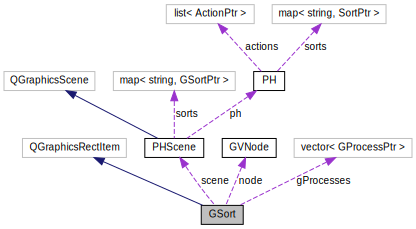
\includegraphics[width=350pt]{classGSort__coll__graph}
\end{center}
\end{figure}
\subsection*{Public Member Functions}
\begin{DoxyCompactItemize}
\item 
\hyperlink{classGSort_a944275172f65a74c9e87bec7032a7637}{G\+Sort} (Sort\+Ptr p, \hyperlink{structGVNode}{G\+V\+Node} n, qreal width, qreal height, \hyperlink{classPHScene}{P\+H\+Scene} $\ast$sc)
\begin{DoxyCompactList}\small\item\em constructor \end{DoxyCompactList}\item 
\hypertarget{classGSort_a06a2e1dd2dec8cad77c17ceb75c6b93b}{Q\+Graphics\+Rect\+Item $\ast$ \hyperlink{classGSort_a06a2e1dd2dec8cad77c17ceb75c6b93b}{get\+Rect} ()}\label{classGSort_a06a2e1dd2dec8cad77c17ceb75c6b93b}

\begin{DoxyCompactList}\small\item\em get the rect item \end{DoxyCompactList}\item 
void \hyperlink{classGSort_ac3cbef2a811660668cff937f56ca37fe}{mouse\+Press\+Event} (Q\+Graphics\+Scene\+Mouse\+Event $\ast$event)
\begin{DoxyCompactList}\small\item\em Handles mouse press event (handles drag start) \end{DoxyCompactList}\item 
void \hyperlink{classGSort_aad29bd2ba170cd9b89ca80edf3439367}{mouse\+Move\+Event} (Q\+Graphics\+Scene\+Mouse\+Event $\ast$event)
\begin{DoxyCompactList}\small\item\em Handles mouse move event (handles drag) \end{DoxyCompactList}\item 
void \hyperlink{classGSort_a340c92716c90ad010232fdd972902ff0}{mouse\+Release\+Event} (Q\+Graphics\+Scene\+Mouse\+Event $\ast$event)
\begin{DoxyCompactList}\small\item\em Handles mouse release event (handles drop) \end{DoxyCompactList}\item 
void \hyperlink{classGSort_ad91eafb0a2ef415cb9b3f47f9c608da7}{mouse\+Double\+Click\+Event} (Q\+Graphics\+Scene\+Mouse\+Event $\ast$event)
\begin{DoxyCompactList}\small\item\em Handles context menu event (typically on right click) \end{DoxyCompactList}\item 
Sort\+Ptr \hyperlink{classGSort_a69520d78ab078c083b8090f9190424b0}{get\+Sort} ()
\begin{DoxyCompactList}\small\item\em gets the related \hyperlink{classSort}{Sort} object \end{DoxyCompactList}\item 
\hyperlink{structGVNode}{G\+V\+Node} \hyperlink{classGSort_a48ceb7cdbb0392344873fd88395675c4}{get\+Node} ()
\begin{DoxyCompactList}\small\item\em gets the related Node object \end{DoxyCompactList}\item 
\hypertarget{classGSort_a50bd1249aaf2833987b66d950bcc86f6}{Q\+Graphics\+Text\+Item $\ast$ \hyperlink{classGSort_a50bd1249aaf2833987b66d950bcc86f6}{get\+Text} ()}\label{classGSort_a50bd1249aaf2833987b66d950bcc86f6}

\begin{DoxyCompactList}\small\item\em gets the text of the sort \end{DoxyCompactList}\item 
\hypertarget{classGSort_a71720b5ffb72f15a896637d572d97497}{Q\+Point \hyperlink{classGSort_a71720b5ffb72f15a896637d572d97497}{getevent\+Press\+Point} ()}\label{classGSort_a71720b5ffb72f15a896637d572d97497}

\begin{DoxyCompactList}\small\item\em gets the point used to record mouse press event position \end{DoxyCompactList}\item 
Q\+Point\+F $\ast$ \hyperlink{classGSort_ae795196b315650b96660693bcc7ce877}{get\+Left\+Top\+Corner\+Point} ()
\begin{DoxyCompactList}\small\item\em get the left top corner of the \hyperlink{classGSort}{G\+Sort} \end{DoxyCompactList}\item 
Q\+Point\+F \hyperlink{classGSort_aaa3431ebe3238fdf1d118a98316a0396}{get\+Center\+Point} ()
\begin{DoxyCompactList}\small\item\em get the center of the \hyperlink{classGSort}{G\+Sort} \end{DoxyCompactList}\item 
Q\+Size $\ast$ \hyperlink{classGSort_af38ef8c716b6566c862790a9039b38c4}{get\+Size\+Rect} ()
\begin{DoxyCompactList}\small\item\em get the size of the ellipse representing the process \end{DoxyCompactList}\item 
vector$<$ G\+Process\+Ptr $>$ \hyperlink{classGSort_acf62f4e6978631b1c714a74cdd0a156e}{get\+G\+Processes} ()
\begin{DoxyCompactList}\small\item\em get the simple display state \end{DoxyCompactList}\item 
\hypertarget{classGSort_a962c988b33337528415e98faca813bc1}{bool {\bfseries get\+Simple\+Display} ()}\label{classGSort_a962c988b33337528415e98faca813bc1}

\item 
\hypertarget{classGSort_ad2656e5a0ec4494845446839105a6a38}{void {\bfseries change\+Display\+State} ()}\label{classGSort_ad2656e5a0ec4494845446839105a6a38}

\item 
void \hyperlink{classGSort_a8fb117049ba9dd1c0a98bdfe44d2b647}{set\+Simple\+Display} (bool is\+Simple\+Display)
\begin{DoxyCompactList}\small\item\em setters for simple\+Display attributes \end{DoxyCompactList}\item 
\hypertarget{classGSort_acafeaec8637b62aea47c2ecb4c36e0be}{void \hyperlink{classGSort_acafeaec8637b62aea47c2ecb4c36e0be}{hide} ()}\label{classGSort_acafeaec8637b62aea47c2ecb4c36e0be}

\begin{DoxyCompactList}\small\item\em hides this \hyperlink{classGSort}{G\+Sort} setting opacity to 0 \end{DoxyCompactList}\item 
\hypertarget{classGSort_a0d487a46aa66f74d68b68e54158b4979}{void {\bfseries actions\+Hide} ()}\label{classGSort_a0d487a46aa66f74d68b68e54158b4979}

\item 
\hypertarget{classGSort_a6cb13a9b6ef35dc7698b165ff0d34b88}{void \hyperlink{classGSort_a6cb13a9b6ef35dc7698b165ff0d34b88}{show} ()}\label{classGSort_a6cb13a9b6ef35dc7698b165ff0d34b88}

\begin{DoxyCompactList}\small\item\em show the \hyperlink{classGSort}{G\+Sort} setting full opacity \end{DoxyCompactList}\item 
\hypertarget{classGSort_a4034d89e182ef3b925943a7502f86bea}{void {\bfseries actions\+Show} ()}\label{classGSort_a4034d89e182ef3b925943a7502f86bea}

\item 
\hypertarget{classGSort_a58e2a6099a59b26ffe7dafd90590bd3d}{bool \hyperlink{classGSort_a58e2a6099a59b26ffe7dafd90590bd3d}{is\+Visible} ()}\label{classGSort_a58e2a6099a59b26ffe7dafd90590bd3d}

\begin{DoxyCompactList}\small\item\em indicates whether or not this \hyperlink{classGSort}{G\+Sort} is made visible (test based on opacity, cf. \hyperlink{classGSort_acafeaec8637b62aea47c2ecb4c36e0be}{hide()} and \hyperlink{classGSort_a6cb13a9b6ef35dc7698b165ff0d34b88}{show()}) \end{DoxyCompactList}\item 
bool \hyperlink{classGSort_adc28cc76ca52518252608fb37ff485ea}{is\+Vertical} ()
\begin{DoxyCompactList}\small\item\em return the value of the vertical attribute \end{DoxyCompactList}\item 
\hypertarget{classGSort_ab9f808442b0bc03573566deaec8fa3f8}{bool \hyperlink{classGSort_ab9f808442b0bc03573566deaec8fa3f8}{is\+Bold} ()}\label{classGSort_ab9f808442b0bc03573566deaec8fa3f8}

\begin{DoxyCompactList}\small\item\em indicates whether or not this \hyperlink{classGSort}{G\+Sort} is made in bold \end{DoxyCompactList}\item 
\hypertarget{classGSort_a949ab093cfc0c732777eb086eab4f14d}{void \hyperlink{classGSort_a949ab093cfc0c732777eb086eab4f14d}{to\+Bold} ()}\label{classGSort_a949ab093cfc0c732777eb086eab4f14d}

\begin{DoxyCompactList}\small\item\em change this \hyperlink{classGSort}{G\+Sort} to bold \end{DoxyCompactList}\item 
\hypertarget{classGSort_a2b6ddd556e6314b3a5be157c41be2c05}{void \hyperlink{classGSort_a2b6ddd556e6314b3a5be157c41be2c05}{Actions\+In\+To\+Bold} ()}\label{classGSort_a2b6ddd556e6314b3a5be157c41be2c05}

\begin{DoxyCompactList}\small\item\em change the G\+Actions In of this \hyperlink{classSort}{Sort} to bold \end{DoxyCompactList}\item 
\hypertarget{classGSort_ae09c5f8af47355ef2328e28fa4d4e834}{void \hyperlink{classGSort_ae09c5f8af47355ef2328e28fa4d4e834}{Actions\+Out\+To\+Bold} ()}\label{classGSort_ae09c5f8af47355ef2328e28fa4d4e834}

\begin{DoxyCompactList}\small\item\em change the G\+Actions out of this \hyperlink{classSort}{Sort} to bold \end{DoxyCompactList}\item 
\hypertarget{classGSort_a6db06cbba4b129e8dc437f26782ae6a1}{void \hyperlink{classGSort_a6db06cbba4b129e8dc437f26782ae6a1}{Actions\+In\+Change\+Color} ()}\label{classGSort_a6db06cbba4b129e8dc437f26782ae6a1}

\begin{DoxyCompactList}\small\item\em change the G\+Actions In color \end{DoxyCompactList}\item 
\hypertarget{classGSort_a6a8db6207e236cef662c54b7432f7aca}{void \hyperlink{classGSort_a6a8db6207e236cef662c54b7432f7aca}{Actions\+Out\+Change\+Color} ()}\label{classGSort_a6a8db6207e236cef662c54b7432f7aca}

\begin{DoxyCompactList}\small\item\em change the G\+Actions out color \end{DoxyCompactList}\item 
\hypertarget{classGSort_afbcbe962474f11f1aa25c215c4c334dc}{void \hyperlink{classGSort_afbcbe962474f11f1aa25c215c4c334dc}{process\+Change\+Color} ()}\label{classGSort_afbcbe962474f11f1aa25c215c4c334dc}

\begin{DoxyCompactList}\small\item\em change the process color \end{DoxyCompactList}\item 
\hypertarget{classGSort_a527cc68e3c8084562803f9411cc9f4b0}{void \hyperlink{classGSort_a527cc68e3c8084562803f9411cc9f4b0}{process\+Change\+Border\+Color} ()}\label{classGSort_a527cc68e3c8084562803f9411cc9f4b0}

\begin{DoxyCompactList}\small\item\em change the process border color \end{DoxyCompactList}\end{DoxyCompactItemize}
\subsection*{Public Attributes}
\begin{DoxyCompactItemize}
\item 
\hypertarget{classGSort_afdedfe6a6028c586a755315351eee309}{Q\+Color $\ast$ \hyperlink{classGSort_afdedfe6a6028c586a755315351eee309}{color}}\label{classGSort_afdedfe6a6028c586a755315351eee309}

\begin{DoxyCompactList}\small\item\em the color used by the Actions that have this \hyperlink{classSort}{Sort} as source \end{DoxyCompactList}\end{DoxyCompactItemize}
\subsection*{Static Public Attributes}
\begin{DoxyCompactItemize}
\item 
\hypertarget{classGSort_a17bdbcd4d2c88f106390628415c8dac8}{static const int {\bfseries margin\+Default} = 10}\label{classGSort_a17bdbcd4d2c88f106390628415c8dac8}

\item 
\hypertarget{classGSort_a00302d36929b2d641d11a0dbf3bca334}{static const int {\bfseries default\+Distance} = 25}\label{classGSort_a00302d36929b2d641d11a0dbf3bca334}

\end{DoxyCompactItemize}
\subsection*{Protected Member Functions}
\begin{DoxyCompactItemize}
\item 
\hypertarget{classGSort_a52469c9320660f61947a5dbacafbf364}{void \hyperlink{classGSort_a52469c9320660f61947a5dbacafbf364}{init\+Inner\+Attributes} ()}\label{classGSort_a52469c9320660f61947a5dbacafbf364}

\begin{DoxyCompactList}\small\item\em initialize inner attributes of the \hyperlink{classGSort}{G\+Sort} \end{DoxyCompactList}\item 
void \hyperlink{classGSort_afa2425ce7e23102d97a9084fb1e5eb74}{init\+Geometric\+Attributes} (Q\+Size size)
\begin{DoxyCompactList}\small\item\em initialize geometrics attributes of the \hyperlink{classGSort}{G\+Sort} \end{DoxyCompactList}\item 
\hypertarget{classGSort_a372e86482111d1b5405a77b7cee09bff}{void \hyperlink{classGSort_a372e86482111d1b5405a77b7cee09bff}{init\+Rect\+Item} ()}\label{classGSort_a372e86482111d1b5405a77b7cee09bff}

\begin{DoxyCompactList}\small\item\em initialize the \+\_\+rect item of the \hyperlink{classGSort}{G\+Sort} \end{DoxyCompactList}\item 
\hypertarget{classGSort_a72a0d9205b2ca98cd827377d5e4bb9f4}{void \hyperlink{classGSort_a72a0d9205b2ca98cd827377d5e4bb9f4}{init\+Text\+Item} ()}\label{classGSort_a72a0d9205b2ca98cd827377d5e4bb9f4}

\begin{DoxyCompactList}\small\item\em initialize the label of the \hyperlink{classGSort}{G\+Sort} \end{DoxyCompactList}\item 
\hypertarget{classGSort_adb374fdb97d1c2ed47ba46d92a7de298}{void \hyperlink{classGSort_adb374fdb97d1c2ed47ba46d92a7de298}{init\+G\+Process\+Children} ()}\label{classGSort_adb374fdb97d1c2ed47ba46d92a7de298}

\begin{DoxyCompactList}\small\item\em initialize \hyperlink{classGProcess}{G\+Process} related to the \hyperlink{classGSort}{G\+Sort} \end{DoxyCompactList}\item 
void \hyperlink{classGSort_a74c3c052d111d72784b6ad286ff219b2}{shift\+Position} (Q\+Point\+F shift\+Vector)
\begin{DoxyCompactList}\small\item\em shifts the \hyperlink{classGSort}{G\+Sort} according to the coordinates of a shift\+Vector \end{DoxyCompactList}\item 
bool \hyperlink{classGSort_a43f637ea0c82b59fdda78380f3e46608}{is\+Over\+Another\+G\+Sort} ()
\begin{DoxyCompactList}\small\item\em check if the \hyperlink{classGSort}{G\+Sort} is over another \end{DoxyCompactList}\item 
bool \hyperlink{classGSort_a417e8b227cfb23393b44dc3b75204dbd}{is\+Over} (\hyperlink{classGSort}{G\+Sort} $\ast$other\+G\+Sort)
\begin{DoxyCompactList}\small\item\em check if the \hyperlink{classGSort}{G\+Sort} is over a specified \hyperlink{classGSort}{G\+Sort} \end{DoxyCompactList}\item 
\hypertarget{classGSort_afe21929462477faeaf61dc705e5225f0}{void \hyperlink{classGSort_afe21929462477faeaf61dc705e5225f0}{cancel\+Shift} ()}\label{classGSort_afe21929462477faeaf61dc705e5225f0}

\begin{DoxyCompactList}\small\item\em set the position of the \hyperlink{classGSort}{G\+Sort} at the state before it has moved \end{DoxyCompactList}\item 
\hypertarget{classGSort_af6e2d5c0135d55f8a152ba58fc20f9f2}{void \hyperlink{classGSort_af6e2d5c0135d55f8a152ba58fc20f9f2}{change\+Orientation} ()}\label{classGSort_af6e2d5c0135d55f8a152ba58fc20f9f2}

\begin{DoxyCompactList}\small\item\em change the orientation of the \hyperlink{classGSort}{G\+Sort} \end{DoxyCompactList}\item 
\hypertarget{classGSort_aa4c1345a701c975b34de5405bf4d1ab8}{void \hyperlink{classGSort_aa4c1345a701c975b34de5405bf4d1ab8}{change\+Color} ()}\label{classGSort_aa4c1345a701c975b34de5405bf4d1ab8}

\begin{DoxyCompactList}\small\item\em change the color of the \hyperlink{classGSort}{G\+Sort} \end{DoxyCompactList}\item 
\hypertarget{classGSort_a2c14e5aa71f7353f18700819f038e542}{void \hyperlink{classGSort_a2c14e5aa71f7353f18700819f038e542}{change\+Orientation\+Rect} ()}\label{classGSort_a2c14e5aa71f7353f18700819f038e542}

\begin{DoxyCompactList}\small\item\em change the orientation of the \hyperlink{classGSort}{G\+Sort} rectangle \end{DoxyCompactList}\item 
\hypertarget{classGSort_a7a98e4937870f2b5cceacebc1b3ccfff}{void \hyperlink{classGSort_a7a98e4937870f2b5cceacebc1b3ccfff}{change\+Orientation\+G\+Process} ()}\label{classGSort_a7a98e4937870f2b5cceacebc1b3ccfff}

\begin{DoxyCompactList}\small\item\em change the orientation of the \hyperlink{classGProcess}{G\+Process} children \end{DoxyCompactList}\item 
\hypertarget{classGSort_a4250ae248bbf752f2af240d5c88e3a9b}{void {\bfseries process\+Change\+Bold} ()}\label{classGSort_a4250ae248bbf752f2af240d5c88e3a9b}

\end{DoxyCompactItemize}
\subsection*{Static Protected Member Functions}
\begin{DoxyCompactItemize}
\item 
static Q\+Color $\ast$ \hyperlink{classGSort_a8df1bb3e016f20eaf6f195dc3055e49e}{make\+Color} (void)
\begin{DoxyCompactList}\small\item\em gets a new color in the palette \end{DoxyCompactList}\end{DoxyCompactItemize}
\subsection*{Protected Attributes}
\begin{DoxyCompactItemize}
\item 
\hypertarget{classGSort_a15b874bf036f285664508a85602aa037}{Q\+Point\+F $\ast$ \hyperlink{classGSort_a15b874bf036f285664508a85602aa037}{left\+Top\+Corner}}\label{classGSort_a15b874bf036f285664508a85602aa037}

\begin{DoxyCompactList}\small\item\em position of the left top corner of the rectangle representing the sort \end{DoxyCompactList}\item 
\hypertarget{classGSort_a621da5d2a45083b02a35bce999022079}{Q\+Size $\ast$ \hyperlink{classGSort_a621da5d2a45083b02a35bce999022079}{size\+Rect}}\label{classGSort_a621da5d2a45083b02a35bce999022079}

\begin{DoxyCompactList}\small\item\em size of the rectangle representing the sort \end{DoxyCompactList}\item 
\hypertarget{classGSort_aa5979b4b0c0e9efbccce0de13ded38d8}{Q\+Graphics\+Rect\+Item $\ast$ \hyperlink{classGSort_aa5979b4b0c0e9efbccce0de13ded38d8}{\+\_\+rect}}\label{classGSort_aa5979b4b0c0e9efbccce0de13ded38d8}

\begin{DoxyCompactList}\small\item\em the graphical item representing the rectangle of the \hyperlink{classSort}{Sort} \end{DoxyCompactList}\item 
\hypertarget{classGSort_a17c4f8eafc9402f5393e69e614f5429a}{Q\+Graphics\+Text\+Item $\ast$ \hyperlink{classGSort_a17c4f8eafc9402f5393e69e614f5429a}{text}}\label{classGSort_a17c4f8eafc9402f5393e69e614f5429a}

\begin{DoxyCompactList}\small\item\em the graphical item representing the text of the \hyperlink{classSort}{Sort} \end{DoxyCompactList}\item 
\hypertarget{classGSort_a8dea499c0b3fa30f9e9558a165a52030}{Sort\+Ptr \hyperlink{classGSort_a8dea499c0b3fa30f9e9558a165a52030}{sort}}\label{classGSort_a8dea499c0b3fa30f9e9558a165a52030}

\begin{DoxyCompactList}\small\item\em the related \hyperlink{classSort}{Sort} \end{DoxyCompactList}\item 
\hypertarget{classGSort_ae76c81595f0c9d39ef35dfc2b72cd42e}{vector$<$ G\+Process\+Ptr $>$ \hyperlink{classGSort_ae76c81595f0c9d39ef35dfc2b72cd42e}{g\+Processes}}\label{classGSort_ae76c81595f0c9d39ef35dfc2b72cd42e}

\begin{DoxyCompactList}\small\item\em list of G\+Process\+Ptr contained by the sort \end{DoxyCompactList}\item 
\hypertarget{classGSort_a8c14e3fef61ee8c44127f285ab04ca5b}{\hyperlink{structGVNode}{G\+V\+Node} \hyperlink{classGSort_a8c14e3fef61ee8c44127f285ab04ca5b}{node}}\label{classGSort_a8c14e3fef61ee8c44127f285ab04ca5b}

\begin{DoxyCompactList}\small\item\em the related of the skeleton\+Graph \end{DoxyCompactList}\item 
\hypertarget{classGSort_a0985310dc8c415f5ac015cde3a28d6a3}{Q\+Point \hyperlink{classGSort_a0985310dc8c415f5ac015cde3a28d6a3}{init\+Pos\+Point}}\label{classGSort_a0985310dc8c415f5ac015cde3a28d6a3}

\begin{DoxyCompactList}\small\item\em the point used to record this \hyperlink{classGSort}{G\+Sort}'s coordinates when user clicks it (ie. starts drag\&drop) \end{DoxyCompactList}\item 
\hypertarget{classGSort_ad33260958b9f1fdea916b737dedc5ba7}{Q\+Point \hyperlink{classGSort_ad33260958b9f1fdea916b737dedc5ba7}{event\+Press\+Point}}\label{classGSort_ad33260958b9f1fdea916b737dedc5ba7}

\begin{DoxyCompactList}\small\item\em the point used to record mouse press event position \end{DoxyCompactList}\item 
\hypertarget{classGSort_a92702d91a49f5a4aadf387e6b10c664a}{qreal \hyperlink{classGSort_a92702d91a49f5a4aadf387e6b10c664a}{padding\+Top}}\label{classGSort_a92702d91a49f5a4aadf387e6b10c664a}

\begin{DoxyCompactList}\small\item\em the space between this \hyperlink{classGSort}{G\+Sort}'s top side and the top \hyperlink{classGProcess}{G\+Process} \end{DoxyCompactList}\item 
\hypertarget{classGSort_ab420d44edd3759c7afbc30fb9d6e9f4f}{bool \hyperlink{classGSort_ab420d44edd3759c7afbc30fb9d6e9f4f}{vertical}}\label{classGSort_ab420d44edd3759c7afbc30fb9d6e9f4f}

\begin{DoxyCompactList}\small\item\em if the sort is vertical or not \end{DoxyCompactList}\item 
\hypertarget{classGSort_a58c1714d20b3eb4bec30b2989cef4a1b}{bool \hyperlink{classGSort_a58c1714d20b3eb4bec30b2989cef4a1b}{bold}}\label{classGSort_a58c1714d20b3eb4bec30b2989cef4a1b}

\begin{DoxyCompactList}\small\item\em if the sort is in bold or not \end{DoxyCompactList}\item 
\hypertarget{classGSort_ac8cb95ac18d2382bf37feb664c885175}{bool \hyperlink{classGSort_ac8cb95ac18d2382bf37feb664c885175}{simple\+Display}}\label{classGSort_ac8cb95ac18d2382bf37feb664c885175}

\begin{DoxyCompactList}\small\item\em if action related to this sort has to be displayed following the simplified model \end{DoxyCompactList}\item 
\hypertarget{classGSort_a7d2304aa3500975d1ecb4480c5d15267}{bool \hyperlink{classGSort_a7d2304aa3500975d1ecb4480c5d15267}{is\+Right\+Button\+Pressed}}\label{classGSort_a7d2304aa3500975d1ecb4480c5d15267}

\begin{DoxyCompactList}\small\item\em to know if the right button of the mouse is pressed (to prevent drag'n'drop in this case) \end{DoxyCompactList}\item 
\hypertarget{classGSort_a35c5f76dda2b7eca466101888f5d4a20}{\hyperlink{classPHScene}{P\+H\+Scene} $\ast$ {\bfseries scene}}\label{classGSort_a35c5f76dda2b7eca466101888f5d4a20}

\end{DoxyCompactItemize}
\subsection*{Static Protected Attributes}
\begin{DoxyCompactItemize}
\item 
static std\+::vector$<$ Q\+Color $>$ \hyperlink{classGSort_a5ca0e05b99745151c30e4d44b3c4564d}{palette}
\begin{DoxyCompactList}\small\item\em the palette of colors that may be used as color member \end{DoxyCompactList}\item 
\hypertarget{classGSort_a684c424c03a77a4f60b88f98021bb2eb}{static int \hyperlink{classGSort_a684c424c03a77a4f60b88f98021bb2eb}{palette\+Index} = 0}\label{classGSort_a684c424c03a77a4f60b88f98021bb2eb}

\begin{DoxyCompactList}\small\item\em palette management index \end{DoxyCompactList}\end{DoxyCompactItemize}


\subsection{Detailed Description}
contains style and layout info to draw a \hyperlink{classSort}{Sort} 

Definition at line 32 of file G\+Sort.\+h.



\subsection{Constructor \& Destructor Documentation}
\hypertarget{classGSort_a944275172f65a74c9e87bec7032a7637}{\index{G\+Sort@{G\+Sort}!G\+Sort@{G\+Sort}}
\index{G\+Sort@{G\+Sort}!G\+Sort@{G\+Sort}}
\subsubsection[{G\+Sort}]{\setlength{\rightskip}{0pt plus 5cm}G\+Sort\+::\+G\+Sort (
\begin{DoxyParamCaption}
\item[{Sort\+Ptr}]{p, }
\item[{{\bf G\+V\+Node}}]{n, }
\item[{qreal}]{width, }
\item[{qreal}]{height, }
\item[{{\bf P\+H\+Scene} $\ast$}]{sc}
\end{DoxyParamCaption}
)}}\label{classGSort_a944275172f65a74c9e87bec7032a7637}


constructor 


\begin{DoxyParams}{Parameters}
{\em Sort\+Ptr} & the related \hyperlink{classSort}{Sort} object \\
\hline
{\em \hyperlink{structGVNode}{G\+V\+Node}} & the node of the skeleton graph containing layout info \\
\hline
{\em qreal} & width of the \hyperlink{classSort}{Sort} \\
\hline
{\em qreal} & height of the \hyperlink{classSort}{Sort} \\
\hline
\end{DoxyParams}


Definition at line 22 of file G\+Sort.\+cpp.


\begin{DoxyCode}
22                                                                         : QGraphicsRectItem(n.
      \hyperlink{structGVNode_a2ceb3d0e7d3f164710622acd3cbea6a6}{centerPos}.x()-width/2, n.\hyperlink{structGVNode_a2ceb3d0e7d3f164710622acd3cbea6a6}{centerPos}.y()-height/2, width, height),
      \hyperlink{classGSort_a8dea499c0b3fa30f9e9558a165a52030}{sort}(s), \hyperlink{classGSort_a8c14e3fef61ee8c44127f285ab04ca5b}{node}(n),scene(sc) \{
23 
24     \hyperlink{classGSort_a52469c9320660f61947a5dbacafbf364}{initInnerAttributes}();
25 
26     \hyperlink{classGSort_afa2425ce7e23102d97a9084fb1e5eb74}{initGeometricAttributes}(QSize(width, height));
27 
28     \hyperlink{classGSort_a372e86482111d1b5405a77b7cee09bff}{initRectItem}();
29 
30     \hyperlink{classGSort_a72a0d9205b2ca98cd827377d5e4bb9f4}{initTextItem}();
31 
32     setCursor(QCursor(Qt::OpenHandCursor));
33     setAcceptedMouseButtons(Qt::LeftButton | Qt::RightButton);
34 
35     \hyperlink{classGSort_adb374fdb97d1c2ed47ba46d92a7de298}{initGProcessChildren}();
36 
37 \}
\end{DoxyCode}


\subsection{Member Function Documentation}
\hypertarget{classGSort_aaa3431ebe3238fdf1d118a98316a0396}{\index{G\+Sort@{G\+Sort}!get\+Center\+Point@{get\+Center\+Point}}
\index{get\+Center\+Point@{get\+Center\+Point}!G\+Sort@{G\+Sort}}
\subsubsection[{get\+Center\+Point}]{\setlength{\rightskip}{0pt plus 5cm}Q\+Point\+F G\+Sort\+::get\+Center\+Point (
\begin{DoxyParamCaption}
{}
\end{DoxyParamCaption}
)}}\label{classGSort_aaa3431ebe3238fdf1d118a98316a0396}


get the center of the \hyperlink{classGSort}{G\+Sort} 

\begin{DoxyReturn}{Returns}
G\+Point\+F center of the \hyperlink{classGSort}{G\+Sort} 
\end{DoxyReturn}


Definition at line 265 of file G\+Sort.\+cpp.


\begin{DoxyCode}
265                               \{
266     \textcolor{keywordflow}{return} QPoint(\hyperlink{classGSort_a15b874bf036f285664508a85602aa037}{leftTopCorner}->x()+\hyperlink{classGSort_a621da5d2a45083b02a35bce999022079}{sizeRect}->width()/2.0,
      \hyperlink{classGSort_a15b874bf036f285664508a85602aa037}{leftTopCorner}->y()+\hyperlink{classGSort_a621da5d2a45083b02a35bce999022079}{sizeRect}->height()/2.0);
267 \}
\end{DoxyCode}
\hypertarget{classGSort_acf62f4e6978631b1c714a74cdd0a156e}{\index{G\+Sort@{G\+Sort}!get\+G\+Processes@{get\+G\+Processes}}
\index{get\+G\+Processes@{get\+G\+Processes}!G\+Sort@{G\+Sort}}
\subsubsection[{get\+G\+Processes}]{\setlength{\rightskip}{0pt plus 5cm}vector$<$ G\+Process\+Ptr $>$ G\+Sort\+::get\+G\+Processes (
\begin{DoxyParamCaption}
{}
\end{DoxyParamCaption}
)}}\label{classGSort_acf62f4e6978631b1c714a74cdd0a156e}


get the simple display state 

\begin{DoxyReturn}{Returns}
bool value of the attribute simple\+Display 
\end{DoxyReturn}


Definition at line 237 of file G\+Sort.\+cpp.


\begin{DoxyCode}
237                                            \{
238     \textcolor{keywordflow}{return} this->\hyperlink{classGSort_ae76c81595f0c9d39ef35dfc2b72cd42e}{gProcesses};
239 \}
\end{DoxyCode}
\hypertarget{classGSort_ae795196b315650b96660693bcc7ce877}{\index{G\+Sort@{G\+Sort}!get\+Left\+Top\+Corner\+Point@{get\+Left\+Top\+Corner\+Point}}
\index{get\+Left\+Top\+Corner\+Point@{get\+Left\+Top\+Corner\+Point}!G\+Sort@{G\+Sort}}
\subsubsection[{get\+Left\+Top\+Corner\+Point}]{\setlength{\rightskip}{0pt plus 5cm}Q\+Point\+F $\ast$ G\+Sort\+::get\+Left\+Top\+Corner\+Point (
\begin{DoxyParamCaption}
{}
\end{DoxyParamCaption}
)}}\label{classGSort_ae795196b315650b96660693bcc7ce877}


get the left top corner of the \hyperlink{classGSort}{G\+Sort} 

\begin{DoxyReturn}{Returns}
G\+Point\+F$\ast$ a pointer to the left\+Top\+Corner attribute 
\end{DoxyReturn}


Definition at line 261 of file G\+Sort.\+cpp.


\begin{DoxyCode}
261                                       \{
262     \textcolor{keywordflow}{return} this->\hyperlink{classGSort_a15b874bf036f285664508a85602aa037}{leftTopCorner};
263 \}
\end{DoxyCode}
\hypertarget{classGSort_a48ceb7cdbb0392344873fd88395675c4}{\index{G\+Sort@{G\+Sort}!get\+Node@{get\+Node}}
\index{get\+Node@{get\+Node}!G\+Sort@{G\+Sort}}
\subsubsection[{get\+Node}]{\setlength{\rightskip}{0pt plus 5cm}{\bf G\+V\+Node} G\+Sort\+::get\+Node (
\begin{DoxyParamCaption}
{}
\end{DoxyParamCaption}
)}}\label{classGSort_a48ceb7cdbb0392344873fd88395675c4}


gets the related Node object 

\begin{DoxyReturn}{Returns}
G\+Vnode a pointer to the related \hyperlink{classSort}{Sort} object 
\end{DoxyReturn}


Definition at line 249 of file G\+Sort.\+cpp.


\begin{DoxyCode}
249                       \{
250     \textcolor{keywordflow}{return} this->\hyperlink{classGSort_a8c14e3fef61ee8c44127f285ab04ca5b}{node};
251 \}
\end{DoxyCode}
\hypertarget{classGSort_af38ef8c716b6566c862790a9039b38c4}{\index{G\+Sort@{G\+Sort}!get\+Size\+Rect@{get\+Size\+Rect}}
\index{get\+Size\+Rect@{get\+Size\+Rect}!G\+Sort@{G\+Sort}}
\subsubsection[{get\+Size\+Rect}]{\setlength{\rightskip}{0pt plus 5cm}Q\+Size $\ast$ G\+Sort\+::get\+Size\+Rect (
\begin{DoxyParamCaption}
{}
\end{DoxyParamCaption}
)}}\label{classGSort_af38ef8c716b6566c862790a9039b38c4}


get the size of the ellipse representing the process 

\begin{DoxyReturn}{Returns}
G\+Size the size of the ellipse 
\end{DoxyReturn}


Definition at line 269 of file G\+Sort.\+cpp.


\begin{DoxyCode}
269                           \{
270     \textcolor{keywordflow}{return} this->\hyperlink{classGSort_a621da5d2a45083b02a35bce999022079}{sizeRect};
271 \}
\end{DoxyCode}
\hypertarget{classGSort_a69520d78ab078c083b8090f9190424b0}{\index{G\+Sort@{G\+Sort}!get\+Sort@{get\+Sort}}
\index{get\+Sort@{get\+Sort}!G\+Sort@{G\+Sort}}
\subsubsection[{get\+Sort}]{\setlength{\rightskip}{0pt plus 5cm}Sort\+Ptr G\+Sort\+::get\+Sort (
\begin{DoxyParamCaption}
{}
\end{DoxyParamCaption}
)}}\label{classGSort_a69520d78ab078c083b8090f9190424b0}


gets the related \hyperlink{classSort}{Sort} object 

\begin{DoxyReturn}{Returns}
Sort\+Ptr a pointer to the related \hyperlink{classSort}{Sort} object 
\end{DoxyReturn}


Definition at line 245 of file G\+Sort.\+cpp.


\begin{DoxyCode}
245                        \{
246     \textcolor{keywordflow}{return} this->\hyperlink{classGSort_a8dea499c0b3fa30f9e9558a165a52030}{sort};
247 \}
\end{DoxyCode}
\hypertarget{classGSort_afa2425ce7e23102d97a9084fb1e5eb74}{\index{G\+Sort@{G\+Sort}!init\+Geometric\+Attributes@{init\+Geometric\+Attributes}}
\index{init\+Geometric\+Attributes@{init\+Geometric\+Attributes}!G\+Sort@{G\+Sort}}
\subsubsection[{init\+Geometric\+Attributes}]{\setlength{\rightskip}{0pt plus 5cm}void G\+Sort\+::init\+Geometric\+Attributes (
\begin{DoxyParamCaption}
\item[{Q\+Size}]{size}
\end{DoxyParamCaption}
)\hspace{0.3cm}{\ttfamily [protected]}}}\label{classGSort_afa2425ce7e23102d97a9084fb1e5eb74}


initialize geometrics attributes of the \hyperlink{classGSort}{G\+Sort} 


\begin{DoxyParams}{Parameters}
{\em Q\+Size} & size of the \hyperlink{classGSort}{G\+Sort} \\
\hline
\end{DoxyParams}


Definition at line 54 of file G\+Sort.\+cpp.


\begin{DoxyCode}
54                                               \{
55     \hyperlink{classGSort_a621da5d2a45083b02a35bce999022079}{sizeRect} = \textcolor{keyword}{new} QSize(size.width(), size.height());
56     \hyperlink{classGSort_a15b874bf036f285664508a85602aa037}{leftTopCorner} = \textcolor{keyword}{new} QPointF(\hyperlink{classGSort_a8c14e3fef61ee8c44127f285ab04ca5b}{node}.\hyperlink{structGVNode_a2ceb3d0e7d3f164710622acd3cbea6a6}{centerPos}.x()-
      \hyperlink{classGSort_a621da5d2a45083b02a35bce999022079}{sizeRect}->width()/2,\hyperlink{classGSort_a8c14e3fef61ee8c44127f285ab04ca5b}{node}.\hyperlink{structGVNode_a2ceb3d0e7d3f164710622acd3cbea6a6}{centerPos}.y()-\hyperlink{classGSort_a621da5d2a45083b02a35bce999022079}{sizeRect}->height()/2);
57 \}
\end{DoxyCode}
\hypertarget{classGSort_a417e8b227cfb23393b44dc3b75204dbd}{\index{G\+Sort@{G\+Sort}!is\+Over@{is\+Over}}
\index{is\+Over@{is\+Over}!G\+Sort@{G\+Sort}}
\subsubsection[{is\+Over}]{\setlength{\rightskip}{0pt plus 5cm}bool G\+Sort\+::is\+Over (
\begin{DoxyParamCaption}
\item[{{\bf G\+Sort} $\ast$}]{other\+G\+Sort}
\end{DoxyParamCaption}
)\hspace{0.3cm}{\ttfamily [protected]}}}\label{classGSort_a417e8b227cfb23393b44dc3b75204dbd}


check if the \hyperlink{classGSort}{G\+Sort} is over a specified \hyperlink{classGSort}{G\+Sort} 

\begin{DoxyReturn}{Returns}
bool the result of the checking 
\end{DoxyReturn}


Definition at line 332 of file G\+Sort.\+cpp.


\begin{DoxyCode}
332                                     \{
333     QPointF centerSortMoving(\hyperlink{classGSort_aaa3431ebe3238fdf1d118a98316a0396}{getCenterPoint}());
334     QPointF centerSortAround(otherGSort->\hyperlink{classGSort_aaa3431ebe3238fdf1d118a98316a0396}{getCenterPoint}());
335     qreal distanceWidthMin = \hyperlink{classGSort_af38ef8c716b6566c862790a9039b38c4}{getSizeRect}()->width()/2 + otherGSort->
      \hyperlink{classGSort_af38ef8c716b6566c862790a9039b38c4}{getSizeRect}()->width()/2 +defaultDistance;
336     qreal distanceHeightMin = \hyperlink{classGSort_af38ef8c716b6566c862790a9039b38c4}{getSizeRect}()->height()/2 + otherGSort->
      \hyperlink{classGSort_af38ef8c716b6566c862790a9039b38c4}{getSizeRect}()->height()/2 +defaultDistance;
337 
338     \textcolor{keywordtype}{bool} xCond = abs(centerSortMoving.x()-centerSortAround.x())<distanceWidthMin;
339     \textcolor{keywordtype}{bool} yCond = abs(centerSortMoving.y()-centerSortAround.y())<distanceHeightMin;
340 
341     \textcolor{keywordflow}{return} xCond && yCond;
342 \}
\end{DoxyCode}
\hypertarget{classGSort_a43f637ea0c82b59fdda78380f3e46608}{\index{G\+Sort@{G\+Sort}!is\+Over\+Another\+G\+Sort@{is\+Over\+Another\+G\+Sort}}
\index{is\+Over\+Another\+G\+Sort@{is\+Over\+Another\+G\+Sort}!G\+Sort@{G\+Sort}}
\subsubsection[{is\+Over\+Another\+G\+Sort}]{\setlength{\rightskip}{0pt plus 5cm}bool G\+Sort\+::is\+Over\+Another\+G\+Sort (
\begin{DoxyParamCaption}
{}
\end{DoxyParamCaption}
)\hspace{0.3cm}{\ttfamily [protected]}}}\label{classGSort_a43f637ea0c82b59fdda78380f3e46608}


check if the \hyperlink{classGSort}{G\+Sort} is over another 

\begin{DoxyReturn}{Returns}
bool the result of the checking 
\end{DoxyReturn}


Definition at line 317 of file G\+Sort.\+cpp.


\begin{DoxyCode}
317                                \{
318     map<string, GSortPtr> listGSorts =scene->\hyperlink{classPHScene_a4c7995ab5b0807000aa1234edbb44794}{getGSorts}();
319     \textcolor{keywordtype}{bool} resetPosition = \textcolor{keyword}{false};
320 
321     \textcolor{keywordflow}{for}(\textcolor{keyword}{auto} &s : listGSorts) \{
322         \textcolor{keywordflow}{if}(s.second.get()->getSort()->getName()!=\hyperlink{classGSort_a8dea499c0b3fa30f9e9558a165a52030}{sort}->getName()) \{
323             \textcolor{keywordflow}{if}(\hyperlink{classGSort_a417e8b227cfb23393b44dc3b75204dbd}{isOver}(s.second.get())) \{
324                 resetPosition = \textcolor{keyword}{true};
325             \}
326         \}
327     \}
328 
329     \textcolor{keywordflow}{return} resetPosition;
330 \}
\end{DoxyCode}
\hypertarget{classGSort_adc28cc76ca52518252608fb37ff485ea}{\index{G\+Sort@{G\+Sort}!is\+Vertical@{is\+Vertical}}
\index{is\+Vertical@{is\+Vertical}!G\+Sort@{G\+Sort}}
\subsubsection[{is\+Vertical}]{\setlength{\rightskip}{0pt plus 5cm}bool G\+Sort\+::is\+Vertical (
\begin{DoxyParamCaption}
{}
\end{DoxyParamCaption}
)}}\label{classGSort_adc28cc76ca52518252608fb37ff485ea}


return the value of the vertical attribute 

\begin{DoxyReturn}{Returns}
bool value of the vertical attribute 
\end{DoxyReturn}


Definition at line 499 of file G\+Sort.\+cpp.


\begin{DoxyCode}
499                        \{
500     \textcolor{keywordflow}{return} \hyperlink{classGSort_ab420d44edd3759c7afbc30fb9d6e9f4f}{vertical};
501 \}
\end{DoxyCode}
\hypertarget{classGSort_a8df1bb3e016f20eaf6f195dc3055e49e}{\index{G\+Sort@{G\+Sort}!make\+Color@{make\+Color}}
\index{make\+Color@{make\+Color}!G\+Sort@{G\+Sort}}
\subsubsection[{make\+Color}]{\setlength{\rightskip}{0pt plus 5cm}Q\+Color $\ast$ G\+Sort\+::make\+Color (
\begin{DoxyParamCaption}
\item[{void}]{}
\end{DoxyParamCaption}
)\hspace{0.3cm}{\ttfamily [static]}, {\ttfamily [protected]}}}\label{classGSort_a8df1bb3e016f20eaf6f195dc3055e49e}


gets a new color in the palette 

\begin{DoxyReturn}{Returns}
Q\+Color$\ast$ the color retrieved in the palette 
\end{DoxyReturn}


Definition at line 610 of file G\+Sort.\+cpp.


\begin{DoxyCode}
610                           \{
611     \hyperlink{classGSort_a684c424c03a77a4f60b88f98021bb2eb}{paletteIndex} = (\hyperlink{classGSort_a684c424c03a77a4f60b88f98021bb2eb}{paletteIndex} + 1) % \hyperlink{classGSort_a5ca0e05b99745151c30e4d44b3c4564d}{palette}.size();
612     \textcolor{keywordflow}{return} &(\hyperlink{classGSort_a5ca0e05b99745151c30e4d44b3c4564d}{palette}[\hyperlink{classGSort_a684c424c03a77a4f60b88f98021bb2eb}{paletteIndex}]);
613 \}
\end{DoxyCode}
\hypertarget{classGSort_ad91eafb0a2ef415cb9b3f47f9c608da7}{\index{G\+Sort@{G\+Sort}!mouse\+Double\+Click\+Event@{mouse\+Double\+Click\+Event}}
\index{mouse\+Double\+Click\+Event@{mouse\+Double\+Click\+Event}!G\+Sort@{G\+Sort}}
\subsubsection[{mouse\+Double\+Click\+Event}]{\setlength{\rightskip}{0pt plus 5cm}void G\+Sort\+::mouse\+Double\+Click\+Event (
\begin{DoxyParamCaption}
\item[{Q\+Graphics\+Scene\+Mouse\+Event $\ast$}]{event}
\end{DoxyParamCaption}
)}}\label{classGSort_ad91eafb0a2ef415cb9b3f47f9c608da7}


Handles context menu event (typically on right click) 


\begin{DoxyParams}{Parameters}
{\em Q\+Graphics\+Scene\+Context\+Menu\+Event} & the event to be handled \\
\hline
\end{DoxyParams}


Definition at line 231 of file G\+Sort.\+cpp.


\begin{DoxyCode}
231                                                                  \{
232     changeDisplayState();
233     \textcolor{keyword}{event}->accept();
234 \}
\end{DoxyCode}
\hypertarget{classGSort_aad29bd2ba170cd9b89ca80edf3439367}{\index{G\+Sort@{G\+Sort}!mouse\+Move\+Event@{mouse\+Move\+Event}}
\index{mouse\+Move\+Event@{mouse\+Move\+Event}!G\+Sort@{G\+Sort}}
\subsubsection[{mouse\+Move\+Event}]{\setlength{\rightskip}{0pt plus 5cm}void G\+Sort\+::mouse\+Move\+Event (
\begin{DoxyParamCaption}
\item[{Q\+Graphics\+Scene\+Mouse\+Event $\ast$}]{event}
\end{DoxyParamCaption}
)}}\label{classGSort_aad29bd2ba170cd9b89ca80edf3439367}


Handles mouse move event (handles drag) 


\begin{DoxyParams}{Parameters}
{\em Q\+Graphics\+Scene\+Mouse\+Event} & the event to be handled \\
\hline
\end{DoxyParams}


Definition at line 184 of file G\+Sort.\+cpp.


\begin{DoxyCode}
184                                                           \{
185 
186     QPen pen;
187     pen.setWidth(5);
188     pen.setBrush(Qt::yellow);
189     \hyperlink{classGSort_aa5979b4b0c0e9efbccce0de13ded38d8}{\_rect}->setPen(pen);
190     QPointF eventScenePos(event->scenePos());
191 
192     \textcolor{keywordflow}{if} (\hyperlink{classGSort_a7d2304aa3500975d1ecb4480c5d15267}{isRightButtonPressed}) \{
193         \textcolor{keyword}{event}->ignore();
194         \textcolor{keywordflow}{return};
195     \}
196 
197     \textcolor{comment}{// update item position}
198 
199     QPointF shiftPoint = eventScenePos-\hyperlink{classGSort_ad33260958b9f1fdea916b737dedc5ba7}{eventPressPoint};
200     \hyperlink{classGSort_a74c3c052d111d72784b6ad286ff219b2}{shiftPosition}(shiftPoint);
201 
202     eventPressPoint.setX(event->scenePos().x());
203     eventPressPoint.setY(event->scenePos().y());
204 
205     \textcolor{keyword}{event}->accept();
206 
207 \}
\end{DoxyCode}
\hypertarget{classGSort_ac3cbef2a811660668cff937f56ca37fe}{\index{G\+Sort@{G\+Sort}!mouse\+Press\+Event@{mouse\+Press\+Event}}
\index{mouse\+Press\+Event@{mouse\+Press\+Event}!G\+Sort@{G\+Sort}}
\subsubsection[{mouse\+Press\+Event}]{\setlength{\rightskip}{0pt plus 5cm}void G\+Sort\+::mouse\+Press\+Event (
\begin{DoxyParamCaption}
\item[{Q\+Graphics\+Scene\+Mouse\+Event $\ast$}]{event}
\end{DoxyParamCaption}
)}}\label{classGSort_ac3cbef2a811660668cff937f56ca37fe}


Handles mouse press event (handles drag start) 


\begin{DoxyParams}{Parameters}
{\em Q\+Graphics\+Scene\+Mouse\+Event} & the event to be handled \\
\hline
\end{DoxyParams}


Definition at line 92 of file G\+Sort.\+cpp.


\begin{DoxyCode}
92                                                            \{
93 
94     QPen pen;
95     pen.setWidth(5);
96     pen.setBrush(Qt::yellow);
97     \hyperlink{classGSort_aa5979b4b0c0e9efbccce0de13ded38d8}{\_rect}->setPen(pen);
98 
99     \textcolor{keywordtype}{bool} test=\textcolor{keyword}{true};
100     \textcolor{comment}{// change orientation on right click}
101     \textcolor{keywordflow}{if} (event->button() == Qt::RightButton) \{
102         QMenu menu;
103 
104         QMenu* editSort = menu.addMenu(\textcolor{stringliteral}{"Edit sort"});
105         QAction* switchOrientation = editSort->addAction(\textcolor{stringliteral}{"Switch horizontal/vertical"});
106         QAction* switchDisplay = editSort->addAction(\textcolor{stringliteral}{"Switch to detailled/simple display"});
107         QAction* switchSortBold=editSort->addAction(\textcolor{stringliteral}{"Switch sort to bold/not bold "});
108         QAction* switchSortColor=editSort->addAction(\textcolor{stringliteral}{"Switch sort color "});
109         QAction* hideSort=editSort->addAction(\textcolor{stringliteral}{"Hide sort "});
110 
111         QMenu* editAction = menu.addMenu(\textcolor{stringliteral}{"Edit action"});
112         QMenu* switchActionsIn=editAction->addMenu(\textcolor{stringliteral}{"Switch in actions "});
113         QMenu* switchActionsOut=editAction->addMenu(\textcolor{stringliteral}{"Switch out actions "});
114         QAction* switchActionsInBold=switchActionsIn->addAction(\textcolor{stringliteral}{"Switch Actions in to bold/not bold "});
115         QAction* switchActionsInColor=switchActionsIn->addAction(\textcolor{stringliteral}{"Switch Action in color "});
116         QAction* switchActionsOutBold=switchActionsOut->addAction(\textcolor{stringliteral}{"Switch Action out to bold/not bold "});
117         QAction* switchActionsOutColor=switchActionsOut->addAction(\textcolor{stringliteral}{"Switch Action out color "});
118 
119         QMenu* editProcess=menu.addMenu(\textcolor{stringliteral}{"Edit process"});
120         QAction* switchProcessBold=editProcess->addAction(\textcolor{stringliteral}{"Switch Process to bold/not bold "});
121         QAction* switchProcessColor=editProcess->addAction(\textcolor{stringliteral}{"Switch Process color "});
122         QAction* switchProcesBordersColor=editProcess->addAction(\textcolor{stringliteral}{"Switch Process border color "});
123 
124         QAction* selectedAction = menu.exec(QCursor::pos());
125 
126         \textcolor{keywordflow}{if}(selectedAction != 0) \{
127             \textcolor{keywordflow}{if}(QString::compare(selectedAction->text(),switchOrientation->text())==0) \{
128                 \hyperlink{classGSort_af6e2d5c0135d55f8a152ba58fc20f9f2}{changeOrientation}();
129                 \textcolor{keyword}{event}->accept();
130             \} \textcolor{keywordflow}{else} \textcolor{keywordflow}{if}(QString::compare(selectedAction->text(),switchDisplay->text())==0) \{
131                 changeDisplayState();
132                 \textcolor{keyword}{event}->accept();
133             \} \textcolor{keywordflow}{else} \textcolor{keywordflow}{if}(QString::compare(selectedAction->text(),switchSortColor->text())==0) \{
134                 \hyperlink{classGSort_aa4c1345a701c975b34de5405bf4d1ab8}{changeColor}();
135                 \textcolor{keyword}{event}->accept();
136             \} \textcolor{keywordflow}{else} \textcolor{keywordflow}{if}(QString::compare(selectedAction->text(),switchSortBold->text())==0) \{
137                 \hyperlink{classGSort_a949ab093cfc0c732777eb086eab4f14d}{toBold}();
138                 test=\textcolor{keyword}{false};
139                 \textcolor{keyword}{event}->accept();
140             \} \textcolor{keywordflow}{else} \textcolor{keywordflow}{if}(QString::compare(selectedAction->text(),switchActionsInBold->text())==0) \{
141                 \hyperlink{classGSort_a2b6ddd556e6314b3a5be157c41be2c05}{ActionsInToBold}();
142                 \textcolor{keyword}{event}->accept();
143             \} \textcolor{keywordflow}{else} \textcolor{keywordflow}{if}(QString::compare(selectedAction->text(),switchActionsInColor->text())==0) \{
144                 \hyperlink{classGSort_a6db06cbba4b129e8dc437f26782ae6a1}{ActionsInChangeColor}();
145                 \textcolor{keyword}{event}->accept();
146             \} \textcolor{keywordflow}{else} \textcolor{keywordflow}{if}(QString::compare(selectedAction->text(),switchActionsOutBold->text())==0) \{
147                 \hyperlink{classGSort_ae09c5f8af47355ef2328e28fa4d4e834}{ActionsOutToBold}();
148                 \textcolor{keyword}{event}->accept();
149             \} \textcolor{keywordflow}{else} \textcolor{keywordflow}{if}(QString::compare(selectedAction->text(),switchActionsOutColor->text())==0) \{
150                 \hyperlink{classGSort_a6a8db6207e236cef662c54b7432f7aca}{ActionsOutChangeColor}();
151                 \textcolor{keyword}{event}->accept();
152             \} \textcolor{keywordflow}{else} \textcolor{keywordflow}{if}(QString::compare(selectedAction->text(),switchProcessBold->text())==0) \{
153                 processChangeBold();
154                 \textcolor{keyword}{event}->accept();
155             \} \textcolor{keywordflow}{else} \textcolor{keywordflow}{if}(QString::compare(selectedAction->text(),switchProcessColor->text())==0) \{
156                 \hyperlink{classGSort_afbcbe962474f11f1aa25c215c4c334dc}{processChangeColor}();
157                 \textcolor{keyword}{event}->accept();
158             \} \textcolor{keywordflow}{else} \textcolor{keywordflow}{if}(QString::compare(selectedAction->text(),hideSort->text())==0) \{
159                 this->actionsHide();
160                 \textcolor{keyword}{event}->accept();
161             \} \textcolor{keywordflow}{else} \textcolor{keywordflow}{if}(QString::compare(selectedAction->text(),switchProcesBordersColor->text())==0) \{
162                 \hyperlink{classGSort_a527cc68e3c8084562803f9411cc9f4b0}{processChangeBorderColor}();
163                 \textcolor{keyword}{event}->accept();
164             \}
165             \textcolor{keywordflow}{if}(test) \{
166                 QPen pen;
167                 pen.setWidth(1);
168                 pen.setBrush(Qt::black);
169                 \hyperlink{classGSort_aa5979b4b0c0e9efbccce0de13ded38d8}{\_rect}->setPen(pen);
170             \}
171         \}
172     \} \textcolor{keywordflow}{else} \textcolor{keywordflow}{if} (event->button() == Qt::LeftButton) \{
173         setCursor(QCursor(Qt::ClosedHandCursor));
174         \textcolor{comment}{// record coordinates for drawing item when mouse is moved/released}
175         \hyperlink{classGSort_a0985310dc8c415f5ac015cde3a28d6a3}{initPosPoint}.setX(pos().x());
176         \hyperlink{classGSort_a0985310dc8c415f5ac015cde3a28d6a3}{initPosPoint}.setY(pos().y());
177         \hyperlink{classGSort_ad33260958b9f1fdea916b737dedc5ba7}{eventPressPoint}.setX(event->scenePos().x());
178         \hyperlink{classGSort_ad33260958b9f1fdea916b737dedc5ba7}{eventPressPoint}.setY(event->scenePos().y());
179         \textcolor{keyword}{event}->accept();
180     \}
181 \}
\end{DoxyCode}
\hypertarget{classGSort_a340c92716c90ad010232fdd972902ff0}{\index{G\+Sort@{G\+Sort}!mouse\+Release\+Event@{mouse\+Release\+Event}}
\index{mouse\+Release\+Event@{mouse\+Release\+Event}!G\+Sort@{G\+Sort}}
\subsubsection[{mouse\+Release\+Event}]{\setlength{\rightskip}{0pt plus 5cm}void G\+Sort\+::mouse\+Release\+Event (
\begin{DoxyParamCaption}
\item[{Q\+Graphics\+Scene\+Mouse\+Event $\ast$}]{event}
\end{DoxyParamCaption}
)}}\label{classGSort_a340c92716c90ad010232fdd972902ff0}


Handles mouse release event (handles drop) 


\begin{DoxyParams}{Parameters}
{\em Q\+Graphics\+Scene\+Mouse\+Event} & the event to be handled \\
\hline
\end{DoxyParams}


Definition at line 209 of file G\+Sort.\+cpp.


\begin{DoxyCode}
209                                                              \{
210 
211     \textcolor{keywordflow}{if} (event->button() == Qt::RightButton) \{
212         \hyperlink{classGSort_a7d2304aa3500975d1ecb4480c5d15267}{isRightButtonPressed}=\textcolor{keyword}{false};
213     \}
214 
215     setCursor(QCursor(Qt::OpenHandCursor));
216 
217     \textcolor{keywordflow}{if}(\hyperlink{classGSort_a43f637ea0c82b59fdda78380f3e46608}{isOverAnotherGSort}()) \{
218         \hyperlink{classGSort_afe21929462477faeaf61dc705e5225f0}{cancelShift}();
219     \}
220 
221     \textcolor{keyword}{event}->accept();
222     QPen pen;
223     \textcolor{keywordflow}{if}(\hyperlink{classGSort_a58c1714d20b3eb4bec30b2989cef4a1b}{bold})
224         pen.setWidth(5);
225     \textcolor{keywordflow}{else}
226         pen.setWidth(1);
227     pen.setBrush(Qt::black);
228     \hyperlink{classGSort_aa5979b4b0c0e9efbccce0de13ded38d8}{\_rect}->setPen(pen);
229 \}
\end{DoxyCode}
\hypertarget{classGSort_a8fb117049ba9dd1c0a98bdfe44d2b647}{\index{G\+Sort@{G\+Sort}!set\+Simple\+Display@{set\+Simple\+Display}}
\index{set\+Simple\+Display@{set\+Simple\+Display}!G\+Sort@{G\+Sort}}
\subsubsection[{set\+Simple\+Display}]{\setlength{\rightskip}{0pt plus 5cm}void G\+Sort\+::set\+Simple\+Display (
\begin{DoxyParamCaption}
\item[{bool}]{is\+Simple\+Display}
\end{DoxyParamCaption}
)}}\label{classGSort_a8fb117049ba9dd1c0a98bdfe44d2b647}


setters for simple\+Display attributes 


\begin{DoxyParams}{Parameters}
{\em bool} & value to set simple\+Display to \\
\hline
\end{DoxyParams}


Definition at line 278 of file G\+Sort.\+cpp.


\begin{DoxyCode}
278                                                  \{
279     \textcolor{keywordflow}{if}(this->\hyperlink{classGSort_ac8cb95ac18d2382bf37feb664c885175}{simpleDisplay} != isSimpleDisplay) \{
280         this->changeDisplayState();
281     \}
282 \}
\end{DoxyCode}
\hypertarget{classGSort_a74c3c052d111d72784b6ad286ff219b2}{\index{G\+Sort@{G\+Sort}!shift\+Position@{shift\+Position}}
\index{shift\+Position@{shift\+Position}!G\+Sort@{G\+Sort}}
\subsubsection[{shift\+Position}]{\setlength{\rightskip}{0pt plus 5cm}void G\+Sort\+::shift\+Position (
\begin{DoxyParamCaption}
\item[{Q\+Point\+F}]{shift\+Vector}
\end{DoxyParamCaption}
)\hspace{0.3cm}{\ttfamily [protected]}}}\label{classGSort_a74c3c052d111d72784b6ad286ff219b2}


shifts the \hyperlink{classGSort}{G\+Sort} according to the coordinates of a shift\+Vector 


\begin{DoxyParams}{Parameters}
{\em Q\+Point\+F} & the shifting vector \\
\hline
\end{DoxyParams}


Definition at line 296 of file G\+Sort.\+cpp.


\begin{DoxyCode}
296                                              \{
297 
298     \textcolor{keywordflow}{for}(GProcessPtr &p: \hyperlink{classGSort_ae76c81595f0c9d39ef35dfc2b72cd42e}{gProcesses}) \{
299         qreal prevPosX = p->getCenterPoint()->x();
300         qreal prevPosY = p->getCenterPoint()->y();
301         p->getCenterPoint()->setX(prevPosX + shiftVector.x());
302         p->getCenterPoint()->setY(prevPosY + shiftVector.y());
303     \}
304 
305     \hyperlink{classGSort_a15b874bf036f285664508a85602aa037}{leftTopCorner}->setX(\hyperlink{classGSort_a15b874bf036f285664508a85602aa037}{leftTopCorner}->x() + shiftVector.x());
306     \hyperlink{classGSort_a15b874bf036f285664508a85602aa037}{leftTopCorner}->setY(\hyperlink{classGSort_a15b874bf036f285664508a85602aa037}{leftTopCorner}->y() + shiftVector.y());
307 
308     setPos(x() + shiftVector.x(), y() + shiftVector.y() );
309 
310     scene->\hyperlink{classPHScene_a176668ca3774e8fec7ac7902e70c048e}{updateActions}();
311 \}
\end{DoxyCode}


\subsection{Member Data Documentation}
\hypertarget{classGSort_a5ca0e05b99745151c30e4d44b3c4564d}{\index{G\+Sort@{G\+Sort}!palette@{palette}}
\index{palette@{palette}!G\+Sort@{G\+Sort}}
\subsubsection[{palette}]{\setlength{\rightskip}{0pt plus 5cm}std\+::vector$<$ Q\+Color $>$ G\+Sort\+::palette\hspace{0.3cm}{\ttfamily [static]}, {\ttfamily [protected]}}}\label{classGSort_a5ca0e05b99745151c30e4d44b3c4564d}
{\bfseries Initial value\+:}
\begin{DoxyCode}
=   \{   QColor(181,137,0)
                                            ,   QColor(220,50,47)
                                            ,   QColor(211,54,130)
                                            ,   QColor(108,113,196)
                                            ,   QColor(38,139,210)
                                            ,   QColor(42,161,152)
                                            ,   QColor(133,153,0)
                                      \}
\end{DoxyCode}


the palette of colors that may be used as color member 



Definition at line 267 of file G\+Sort.\+h.



The documentation for this class was generated from the following files\+:\begin{DoxyCompactItemize}
\item 
headers/\hyperlink{GSort_8h}{G\+Sort.\+h}\item 
src/gfx/G\+Sort.\+cpp\end{DoxyCompactItemize}

\hypertarget{structgv__error}{\section{gv\+\_\+error Class Reference}
\label{structgv__error}\index{gv\+\_\+error@{gv\+\_\+error}}
}


struct defining the exception called when an error occurs in Graph\+Viz extends \hyperlink{structexception__base}{exception\+\_\+base}  




{\ttfamily \#include $<$Exceptions.\+h$>$}



Inheritance diagram for gv\+\_\+error\+:\nopagebreak
\begin{figure}[H]
\begin{center}
\leavevmode
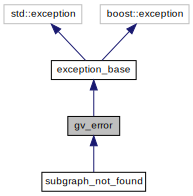
\includegraphics[width=266pt]{structgv__error__inherit__graph}
\end{center}
\end{figure}


Collaboration diagram for gv\+\_\+error\+:\nopagebreak
\begin{figure}[H]
\begin{center}
\leavevmode
\includegraphics[width=266pt]{structgv__error__coll__graph}
\end{center}
\end{figure}


\subsection{Detailed Description}
struct defining the exception called when an error occurs in Graph\+Viz extends \hyperlink{structexception__base}{exception\+\_\+base} 

Definition at line 137 of file Exceptions.\+h.



The documentation for this class was generated from the following file\+:\begin{DoxyCompactItemize}
\item 
headers/\hyperlink{Exceptions_8h}{Exceptions.\+h}\end{DoxyCompactItemize}

\hypertarget{structGVEdge}{\section{G\+V\+Edge Struct Reference}
\label{structGVEdge}\index{G\+V\+Edge@{G\+V\+Edge}}
}


struct containing the information for a G\+V\+Graph's edge  




{\ttfamily \#include $<$G\+V\+Edge.\+h$>$}

\subsection*{Public Attributes}
\begin{DoxyCompactItemize}
\item 
\hypertarget{structGVEdge_a7a3538b20c3747135ce4771be00a3a8a}{Q\+String \hyperlink{structGVEdge_a7a3538b20c3747135ce4771be00a3a8a}{source}}\label{structGVEdge_a7a3538b20c3747135ce4771be00a3a8a}

\begin{DoxyCompactList}\small\item\em the source node of the edge \end{DoxyCompactList}\item 
\hypertarget{structGVEdge_a6883e0ddce3a6fcbde0b01f3645ae7c5}{Q\+String \hyperlink{structGVEdge_a6883e0ddce3a6fcbde0b01f3645ae7c5}{target}}\label{structGVEdge_a6883e0ddce3a6fcbde0b01f3645ae7c5}

\begin{DoxyCompactList}\small\item\em the target node of the edge \end{DoxyCompactList}\item 
\hypertarget{structGVEdge_ad73f00af1e82b13f9c94982327bc9952}{Q\+Painter\+Path \hyperlink{structGVEdge_ad73f00af1e82b13f9c94982327bc9952}{path}}\label{structGVEdge_ad73f00af1e82b13f9c94982327bc9952}

\begin{DoxyCompactList}\small\item\em the path of the edge's line \end{DoxyCompactList}\end{DoxyCompactItemize}


\subsection{Detailed Description}
struct containing the information for a G\+V\+Graph's edge 

Definition at line 18 of file G\+V\+Edge.\+h.



The documentation for this struct was generated from the following file\+:\begin{DoxyCompactItemize}
\item 
headers/\hyperlink{GVEdge_8h}{G\+V\+Edge.\+h}\end{DoxyCompactItemize}

\hypertarget{structGVNode}{\section{G\+V\+Node Struct Reference}
\label{structGVNode}\index{G\+V\+Node@{G\+V\+Node}}
}


struct containing the information for a G\+V\+Graph's node  




{\ttfamily \#include $<$G\+V\+Node.\+h$>$}

\subsection*{Public Attributes}
\begin{DoxyCompactItemize}
\item 
\hypertarget{structGVNode_ad1af9e7c14f0b580854ad3428f1b5c9d}{Q\+String \hyperlink{structGVNode_ad1af9e7c14f0b580854ad3428f1b5c9d}{name}}\label{structGVNode_ad1af9e7c14f0b580854ad3428f1b5c9d}

\begin{DoxyCompactList}\small\item\em the unique identifier of the node in the graph \end{DoxyCompactList}\item 
\hypertarget{structGVNode_a2ceb3d0e7d3f164710622acd3cbea6a6}{Q\+Point \hyperlink{structGVNode_a2ceb3d0e7d3f164710622acd3cbea6a6}{center\+Pos}}\label{structGVNode_a2ceb3d0e7d3f164710622acd3cbea6a6}

\begin{DoxyCompactList}\small\item\em position of the center point of the node from the top-\/left corner \end{DoxyCompactList}\item 
\hypertarget{structGVNode_a498e3f749e2228709a3987ac11512c82}{float \hyperlink{structGVNode_a498e3f749e2228709a3987ac11512c82}{height}}\label{structGVNode_a498e3f749e2228709a3987ac11512c82}

\begin{DoxyCompactList}\small\item\em the size (height and width) of the node in pixels \end{DoxyCompactList}\item 
\hypertarget{structGVNode_adc1d840d0813610c08420ce97195b893}{float {\bfseries width}}\label{structGVNode_adc1d840d0813610c08420ce97195b893}

\end{DoxyCompactItemize}


\subsection{Detailed Description}
struct containing the information for a G\+V\+Graph's node 

Definition at line 17 of file G\+V\+Node.\+h.



The documentation for this struct was generated from the following file\+:\begin{DoxyCompactItemize}
\item 
headers/\hyperlink{GVNode_8h}{G\+V\+Node.\+h}\end{DoxyCompactItemize}

\hypertarget{classGVSkeletonGraph}{\section{G\+V\+Skeleton\+Graph Class Reference}
\label{classGVSkeletonGraph}\index{G\+V\+Skeleton\+Graph@{G\+V\+Skeleton\+Graph}}
}


the object containing a libraph graph representing the skeleton (sorts+actions) of the model and its associated nodes and edges  




{\ttfamily \#include $<$G\+V\+Skeleton\+Graph.\+h$>$}

\subsection*{Public Member Functions}
\begin{DoxyCompactItemize}
\item 
\hyperlink{classGVSkeletonGraph_aff5ae5626bd75ccbb40d54117d6ba379}{G\+V\+Skeleton\+Graph} (Q\+String name, Q\+Font font=Q\+Font())
\begin{DoxyCompactList}\small\item\em \hyperlink{classGVSkeletonGraph}{G\+V\+Skeleton\+Graph} constructor. \end{DoxyCompactList}\item 
\hypertarget{classGVSkeletonGraph_aecb6a116fbb734089ef01ab78580d2d3}{void \hyperlink{classGVSkeletonGraph_aecb6a116fbb734089ef01ab78580d2d3}{set\+Graph\+Attributes} ()}\label{classGVSkeletonGraph_aecb6a116fbb734089ef01ab78580d2d3}

\begin{DoxyCompactList}\small\item\em Set the graph dpi and sep\+Value to their default values. \end{DoxyCompactList}\item 
void \hyperlink{classGVSkeletonGraph_ae47e7e33a02a94658be0ab3c950172bc}{set\+Graph\+Object\+Attributes} (void $\ast$object, Q\+String attr, Q\+String value)
\begin{DoxyCompactList}\small\item\em set an attribute to a given value for a graph element \end{DoxyCompactList}\item 
void \hyperlink{classGVSkeletonGraph_a14ce57fdd94f4f5996af8be2476bf76b}{set\+Font} (Q\+Font font)
\begin{DoxyCompactList}\small\item\em set the font used for the graph \end{DoxyCompactList}\item 
\hypertarget{classGVSkeletonGraph_ade966198333d6aef5f5f56a9849488c9}{void \hyperlink{classGVSkeletonGraph_ade966198333d6aef5f5f56a9849488c9}{apply\+Layout} ()}\label{classGVSkeletonGraph_ade966198333d6aef5f5f56a9849488c9}

\begin{DoxyCompactList}\small\item\em builds the layout \end{DoxyCompactList}\item 
\hypertarget{classGVSkeletonGraph_a53073d1aaae9c5ec6a9dfa04ceb9151b}{void \hyperlink{classGVSkeletonGraph_a53073d1aaae9c5ec6a9dfa04ceb9151b}{export\+To\+Png} ()}\label{classGVSkeletonGraph_a53073d1aaae9c5ec6a9dfa04ceb9151b}

\begin{DoxyCompactList}\small\item\em export the graph into the file out.\+png (for test purpose) \end{DoxyCompactList}\item 
Q\+List$<$ \hyperlink{structGVNode}{G\+V\+Node} $>$ \hyperlink{classGVSkeletonGraph_ac74f8e4b5ad9f207a35eb2696b5740b6}{nodes} ()
\begin{DoxyCompactList}\small\item\em tranforms the \+\_\+nodes attribute into a liste of \hyperlink{structGVNode}{G\+V\+Node} \end{DoxyCompactList}\item 
void \hyperlink{classGVSkeletonGraph_a51513245defe5f4fe3d63b3abc3a220a}{add\+Node} (const Q\+String \&name)
\begin{DoxyCompactList}\small\item\em add a node to the graph \end{DoxyCompactList}\item 
void \hyperlink{classGVSkeletonGraph_a5360f1d472f7c548bcba0b7554dca649}{remove\+Node} (const Q\+String \&name)
\begin{DoxyCompactList}\small\item\em remove a node from the graph \end{DoxyCompactList}\item 
bool \hyperlink{classGVSkeletonGraph_a3488e1b4a133b330835c3c0be7caeedf}{has\+Node} (const Q\+String \&name)
\begin{DoxyCompactList}\small\item\em check if a node exists in the graph \end{DoxyCompactList}\item 
void \hyperlink{classGVSkeletonGraph_a3a283e888b23d526974f860241f8b1cf}{set\+Node\+Size} (void $\ast$object, qreal width, qreal height)
\begin{DoxyCompactList}\small\item\em setter for the node\+Size attribute \end{DoxyCompactList}\item 
Agnode\+\_\+t $\ast$ \hyperlink{classGVSkeletonGraph_adce1790e44da056309d142e153cb5a24}{get\+Node} (const Q\+String \&name)
\begin{DoxyCompactList}\small\item\em gets a node by its name \end{DoxyCompactList}\item 
\hypertarget{classGVSkeletonGraph_a3c1d531da3434485a6556e59c01cf2b5}{void \hyperlink{classGVSkeletonGraph_a3c1d531da3434485a6556e59c01cf2b5}{clear\+Nodes} ()}\label{classGVSkeletonGraph_a3c1d531da3434485a6556e59c01cf2b5}

\begin{DoxyCompactList}\small\item\em remove all nodes of the graph \end{DoxyCompactList}\item 
void \hyperlink{classGVSkeletonGraph_a509442b926cbb771b3e4273574706f13}{add\+Edge} (const Q\+String \&source, const Q\+String \&target)
\begin{DoxyCompactList}\small\item\em add a edge to the graph \end{DoxyCompactList}\item 
void \hyperlink{classGVSkeletonGraph_a1887eb0a40aadf726468b9baf500e58b}{remove\+Edge} (const Q\+String \&source, const Q\+String \&target)
\begin{DoxyCompactList}\small\item\em remove a edge to the graph \end{DoxyCompactList}\item 
void \hyperlink{classGVSkeletonGraph_a546b14e4c3c48b7d0f4eac84955fd360}{remove\+Edge} (const Q\+Pair$<$ Q\+String, Q\+String $>$ \&key)
\begin{DoxyCompactList}\small\item\em remove a edge to the graph \end{DoxyCompactList}\item 
bool \hyperlink{classGVSkeletonGraph_a50d801a00e3c1761c5eb8425982ed345}{connection\+Exists} (const Q\+String \&source\+Name, const Q\+String \&target\+Name)
\begin{DoxyCompactList}\small\item\em check if an edge exists between two nodes in the graph \end{DoxyCompactList}\item 
qreal \hyperlink{classGVSkeletonGraph_abae4623f9d7c1cf8eb078ddc974d8d67}{get\+D\+P\+I} ()
\begin{DoxyCompactList}\small\item\em gets the D\+P\+I value \end{DoxyCompactList}\item 
Agraph\+\_\+t $\ast$ \hyperlink{classGVSkeletonGraph_ade05624b5ad5afd0567af5a394d47011}{graph} ()
\begin{DoxyCompactList}\small\item\em gets the graphviz graph struct of this \hyperlink{classGVSkeletonGraph}{G\+V\+Skeleton\+Graph} \end{DoxyCompactList}\end{DoxyCompactItemize}
\subsection*{Static Public Attributes}
\begin{DoxyCompactItemize}
\item 
\hypertarget{classGVSkeletonGraph_abb7b658c4700d007559323bc62e7c66d}{static const qreal \hyperlink{classGVSkeletonGraph_abb7b658c4700d007559323bc62e7c66d}{Dot\+Default\+D\+P\+I} =72.\+0}\label{classGVSkeletonGraph_abb7b658c4700d007559323bc62e7c66d}

\begin{DoxyCompactList}\small\item\em Default D\+P\+I value used by dot (which uses points instead of pixels for coordinates) \end{DoxyCompactList}\item 
\hypertarget{classGVSkeletonGraph_ad9fe75a063cf1587f81fabeff392885e}{static const qreal \hyperlink{classGVSkeletonGraph_ad9fe75a063cf1587f81fabeff392885e}{node\+Size} = 1}\label{classGVSkeletonGraph_ad9fe75a063cf1587f81fabeff392885e}

\begin{DoxyCompactList}\small\item\em Size in pixels of each node of the skeleton, related to the size of the corresponding \hyperlink{classSort}{Sort}. \end{DoxyCompactList}\item 
\hypertarget{classGVSkeletonGraph_aa660fd51acdd78295969eeee3731339a}{static const qreal \hyperlink{classGVSkeletonGraph_aa660fd51acdd78295969eeee3731339a}{sep\+Value} = 30.\+0}\label{classGVSkeletonGraph_aa660fd51acdd78295969eeee3731339a}

\begin{DoxyCompactList}\small\item\em Minimum margin around each node (in points for graphviz) \end{DoxyCompactList}\end{DoxyCompactItemize}
\subsection*{Protected Attributes}
\begin{DoxyCompactItemize}
\item 
\hypertarget{classGVSkeletonGraph_a09545a121bbd9ef0c0c0a1130f5b11ee}{Q\+Font {\bfseries \+\_\+font}}\label{classGVSkeletonGraph_a09545a121bbd9ef0c0c0a1130f5b11ee}

\item 
\hypertarget{classGVSkeletonGraph_ace0fb45d3ca589997beabf430a889eb8}{G\+V\+C\+\_\+t $\ast$ {\bfseries \+\_\+context}}\label{classGVSkeletonGraph_ace0fb45d3ca589997beabf430a889eb8}

\item 
\hypertarget{classGVSkeletonGraph_abf8e96cecc53806d0fcf5733695b6f0f}{Agraph\+\_\+t $\ast$ {\bfseries \+\_\+graph}}\label{classGVSkeletonGraph_abf8e96cecc53806d0fcf5733695b6f0f}

\item 
\hypertarget{classGVSkeletonGraph_aa56918b8143b0bdb266705cb126cdab8}{Q\+Map$<$ Q\+String, Agnode\+\_\+t $\ast$ $>$ {\bfseries \+\_\+nodes}}\label{classGVSkeletonGraph_aa56918b8143b0bdb266705cb126cdab8}

\item 
\hypertarget{classGVSkeletonGraph_acbf9854e1bf81193cf0617202f2bc868}{Q\+Map$<$ Q\+Pair$<$ Q\+String, Q\+String $>$\\*
, Agedge\+\_\+t $\ast$ $>$ {\bfseries \+\_\+edges}}\label{classGVSkeletonGraph_acbf9854e1bf81193cf0617202f2bc868}

\end{DoxyCompactItemize}


\subsection{Detailed Description}
the object containing a libraph graph representing the skeleton (sorts+actions) of the model and its associated nodes and edges 

Definition at line 27 of file G\+V\+Skeleton\+Graph.\+h.



\subsection{Constructor \& Destructor Documentation}
\hypertarget{classGVSkeletonGraph_aff5ae5626bd75ccbb40d54117d6ba379}{\index{G\+V\+Skeleton\+Graph@{G\+V\+Skeleton\+Graph}!G\+V\+Skeleton\+Graph@{G\+V\+Skeleton\+Graph}}
\index{G\+V\+Skeleton\+Graph@{G\+V\+Skeleton\+Graph}!G\+V\+Skeleton\+Graph@{G\+V\+Skeleton\+Graph}}
\subsubsection[{G\+V\+Skeleton\+Graph}]{\setlength{\rightskip}{0pt plus 5cm}G\+V\+Skeleton\+Graph\+::\+G\+V\+Skeleton\+Graph (
\begin{DoxyParamCaption}
\item[{Q\+String}]{name, }
\item[{Q\+Font}]{font = {\ttfamily QFont()}}
\end{DoxyParamCaption}
)}}\label{classGVSkeletonGraph_aff5ae5626bd75ccbb40d54117d6ba379}


\hyperlink{classGVSkeletonGraph}{G\+V\+Skeleton\+Graph} constructor. 


\begin{DoxyParams}{Parameters}
{\em Q\+String} & name the name given to the skeleton graph \\
\hline
{\em Q\+Font} & font \\
\hline
\end{DoxyParams}


Definition at line 42 of file G\+V\+Skeleton\+Graph.\+cpp.


\begin{DoxyCode}
42                                                          \{
43     setlocale(LC\_NUMERIC,\textcolor{stringliteral}{"en\_US.UTF-8"});
44 
45     \_context = gvContext();
46     \_graph = \_agopen(name, Agstrictdirected);
47     \hyperlink{classGVSkeletonGraph_aecb6a116fbb734089ef01ab78580d2d3}{setGraphAttributes}();
48     \hyperlink{classGVSkeletonGraph_a14ce57fdd94f4f5996af8be2476bf76b}{setFont}(font);
49 \}
\end{DoxyCode}


\subsection{Member Function Documentation}
\hypertarget{classGVSkeletonGraph_a509442b926cbb771b3e4273574706f13}{\index{G\+V\+Skeleton\+Graph@{G\+V\+Skeleton\+Graph}!add\+Edge@{add\+Edge}}
\index{add\+Edge@{add\+Edge}!G\+V\+Skeleton\+Graph@{G\+V\+Skeleton\+Graph}}
\subsubsection[{add\+Edge}]{\setlength{\rightskip}{0pt plus 5cm}void G\+V\+Skeleton\+Graph\+::add\+Edge (
\begin{DoxyParamCaption}
\item[{const Q\+String \&}]{source, }
\item[{const Q\+String \&}]{target}
\end{DoxyParamCaption}
)}}\label{classGVSkeletonGraph_a509442b926cbb771b3e4273574706f13}


add a edge to the graph 


\begin{DoxyParams}{Parameters}
{\em Q\+String} & source the name first node related to the edge \\
\hline
{\em Q\+String} & target the name second node related to the edge \\
\hline
\end{DoxyParams}


Definition at line 171 of file G\+V\+Skeleton\+Graph.\+cpp.


\begin{DoxyCode}
171                                                                           \{
172     setlocale(LC\_NUMERIC,\textcolor{stringliteral}{"en\_US.UTF-8"});
173 
174     \textcolor{keywordflow}{if} (\hyperlink{classGVSkeletonGraph_a3488e1b4a133b330835c3c0be7caeedf}{hasNode}(source) && \hyperlink{classGVSkeletonGraph_a3488e1b4a133b330835c3c0be7caeedf}{hasNode}(target)) \{
175         QPair<QString, QString> key(source, target);
176 
177         \textcolor{keywordflow}{if}(!\_edges.contains(key)) \{
178             Agedge\_t *edge = agedge(\_graph, \hyperlink{classGVSkeletonGraph_adce1790e44da056309d142e153cb5a24}{getNode}(source), \hyperlink{classGVSkeletonGraph_adce1790e44da056309d142e153cb5a24}{getNode}(target), 0, 1);
179             \_edges.insert(key, edge);
180         \}
181 
182     \}
183 \}
\end{DoxyCode}
\hypertarget{classGVSkeletonGraph_a51513245defe5f4fe3d63b3abc3a220a}{\index{G\+V\+Skeleton\+Graph@{G\+V\+Skeleton\+Graph}!add\+Node@{add\+Node}}
\index{add\+Node@{add\+Node}!G\+V\+Skeleton\+Graph@{G\+V\+Skeleton\+Graph}}
\subsubsection[{add\+Node}]{\setlength{\rightskip}{0pt plus 5cm}void G\+V\+Skeleton\+Graph\+::add\+Node (
\begin{DoxyParamCaption}
\item[{const Q\+String \&}]{name}
\end{DoxyParamCaption}
)}}\label{classGVSkeletonGraph_a51513245defe5f4fe3d63b3abc3a220a}


add a node to the graph 


\begin{DoxyParams}{Parameters}
{\em Q\+String} & name the name of the node to add to the graph \\
\hline
\end{DoxyParams}


Definition at line 119 of file G\+V\+Skeleton\+Graph.\+cpp.


\begin{DoxyCode}
119                                                  \{
120     setlocale(LC\_NUMERIC,\textcolor{stringliteral}{"en\_US.UTF-8"});
121 
122     \textcolor{keywordflow}{if}(\_nodes.contains(name)) \hyperlink{classGVSkeletonGraph_a5360f1d472f7c548bcba0b7554dca649}{removeNode}(name);
123 
124     \_nodes.insert(name, \_agnode(\_graph, name));
125 \}
\end{DoxyCode}
\hypertarget{classGVSkeletonGraph_a50d801a00e3c1761c5eb8425982ed345}{\index{G\+V\+Skeleton\+Graph@{G\+V\+Skeleton\+Graph}!connection\+Exists@{connection\+Exists}}
\index{connection\+Exists@{connection\+Exists}!G\+V\+Skeleton\+Graph@{G\+V\+Skeleton\+Graph}}
\subsubsection[{connection\+Exists}]{\setlength{\rightskip}{0pt plus 5cm}bool G\+V\+Skeleton\+Graph\+::connection\+Exists (
\begin{DoxyParamCaption}
\item[{const Q\+String \&}]{source\+Name, }
\item[{const Q\+String \&}]{target\+Name}
\end{DoxyParamCaption}
)}}\label{classGVSkeletonGraph_a50d801a00e3c1761c5eb8425982ed345}


check if an edge exists between two nodes in the graph 


\begin{DoxyParams}{Parameters}
{\em Q\+String} & source the name first node related to the edge \\
\hline
{\em Q\+String} & target the name second node related to the edge \\
\hline
\end{DoxyParams}
\begin{DoxyReturn}{Returns}
bool true if the connection exists, false if it doesn't 
\end{DoxyReturn}


Definition at line 200 of file G\+V\+Skeleton\+Graph.\+cpp.


\begin{DoxyCode}
200                                                                                            \{
201     setlocale(LC\_NUMERIC,\textcolor{stringliteral}{"en\_US.UTF-8"});
202 
203     QPair<QString,QString> firstPossibility(sourceName,targetName);
204     QPair<QString,QString> secondPossibility(targetName,sourceName);
205     \textcolor{keywordflow}{return} \_edges.contains(firstPossibility)||\_edges.contains(secondPossibility);
206 \}
\end{DoxyCode}
\hypertarget{classGVSkeletonGraph_abae4623f9d7c1cf8eb078ddc974d8d67}{\index{G\+V\+Skeleton\+Graph@{G\+V\+Skeleton\+Graph}!get\+D\+P\+I@{get\+D\+P\+I}}
\index{get\+D\+P\+I@{get\+D\+P\+I}!G\+V\+Skeleton\+Graph@{G\+V\+Skeleton\+Graph}}
\subsubsection[{get\+D\+P\+I}]{\setlength{\rightskip}{0pt plus 5cm}qreal G\+V\+Skeleton\+Graph\+::get\+D\+P\+I (
\begin{DoxyParamCaption}
{}
\end{DoxyParamCaption}
)}}\label{classGVSkeletonGraph_abae4623f9d7c1cf8eb078ddc974d8d67}


gets the D\+P\+I value 

\begin{DoxyReturn}{Returns}
qreal the D\+P\+I value 
\end{DoxyReturn}


Definition at line 208 of file G\+V\+Skeleton\+Graph.\+cpp.


\begin{DoxyCode}
208                               \{
209     setlocale(LC\_NUMERIC,\textcolor{stringliteral}{"en\_US.UTF-8"});
210     \textcolor{keywordflow}{return} \_agget(\_graph, \textcolor{stringliteral}{"dpi"},\textcolor{stringliteral}{"96,0"}).replace(\textcolor{charliteral}{','},\textcolor{stringliteral}{"."}).toDouble();
211 \}
\end{DoxyCode}
\hypertarget{classGVSkeletonGraph_adce1790e44da056309d142e153cb5a24}{\index{G\+V\+Skeleton\+Graph@{G\+V\+Skeleton\+Graph}!get\+Node@{get\+Node}}
\index{get\+Node@{get\+Node}!G\+V\+Skeleton\+Graph@{G\+V\+Skeleton\+Graph}}
\subsubsection[{get\+Node}]{\setlength{\rightskip}{0pt plus 5cm}Agnode\+\_\+t $\ast$ G\+V\+Skeleton\+Graph\+::get\+Node (
\begin{DoxyParamCaption}
\item[{const Q\+String \&}]{name}
\end{DoxyParamCaption}
)}}\label{classGVSkeletonGraph_adce1790e44da056309d142e153cb5a24}


gets a node by its name 


\begin{DoxyParams}{Parameters}
{\em Q\+String} & name the name of the node to get \\
\hline
\end{DoxyParams}
\begin{DoxyReturn}{Returns}
Agnode\+\_\+t$\ast$ a pointer to the retrieved node 
\end{DoxyReturn}


Definition at line 143 of file G\+V\+Skeleton\+Graph.\+cpp.


\begin{DoxyCode}
143                                                       \{
144     setlocale(LC\_NUMERIC,\textcolor{stringliteral}{"en\_US.UTF-8"});
145 
146     \textcolor{keywordflow}{if}(\_nodes.contains(name)) \textcolor{keywordflow}{return} \_nodes[name];
147 
148     \textcolor{keywordflow}{return} NULL;
149 \}
\end{DoxyCode}
\hypertarget{classGVSkeletonGraph_ade05624b5ad5afd0567af5a394d47011}{\index{G\+V\+Skeleton\+Graph@{G\+V\+Skeleton\+Graph}!graph@{graph}}
\index{graph@{graph}!G\+V\+Skeleton\+Graph@{G\+V\+Skeleton\+Graph}}
\subsubsection[{graph}]{\setlength{\rightskip}{0pt plus 5cm}Agraph\+\_\+t $\ast$ G\+V\+Skeleton\+Graph\+::graph (
\begin{DoxyParamCaption}
{}
\end{DoxyParamCaption}
)}}\label{classGVSkeletonGraph_ade05624b5ad5afd0567af5a394d47011}


gets the graphviz graph struct of this \hyperlink{classGVSkeletonGraph}{G\+V\+Skeleton\+Graph} 

\begin{DoxyReturn}{Returns}
Agraph\+\_\+t$\ast$ a pointer to the graph 
\end{DoxyReturn}


Definition at line 213 of file G\+V\+Skeleton\+Graph.\+cpp.


\begin{DoxyCode}
213                                  \{
214     setlocale(LC\_NUMERIC,\textcolor{stringliteral}{"en\_US.UTF-8"});
215     \textcolor{keywordflow}{return} this->\_graph;
216 \}
\end{DoxyCode}
\hypertarget{classGVSkeletonGraph_a3488e1b4a133b330835c3c0be7caeedf}{\index{G\+V\+Skeleton\+Graph@{G\+V\+Skeleton\+Graph}!has\+Node@{has\+Node}}
\index{has\+Node@{has\+Node}!G\+V\+Skeleton\+Graph@{G\+V\+Skeleton\+Graph}}
\subsubsection[{has\+Node}]{\setlength{\rightskip}{0pt plus 5cm}bool G\+V\+Skeleton\+Graph\+::has\+Node (
\begin{DoxyParamCaption}
\item[{const Q\+String \&}]{name}
\end{DoxyParamCaption}
)}}\label{classGVSkeletonGraph_a3488e1b4a133b330835c3c0be7caeedf}


check if a node exists in the graph 


\begin{DoxyParams}{Parameters}
{\em Q\+String} & name the name of the node which existence is to be checked \\
\hline
\end{DoxyParams}


Definition at line 136 of file G\+V\+Skeleton\+Graph.\+cpp.


\begin{DoxyCode}
136                                                  \{
137     setlocale(LC\_NUMERIC,\textcolor{stringliteral}{"en\_US.UTF-8"});
138 
139     \textcolor{keywordflow}{if}(\_nodes.contains(name)) \textcolor{keywordflow}{return} \textcolor{keyword}{true};
140     \textcolor{keywordflow}{return} \textcolor{keyword}{false};
141 \}
\end{DoxyCode}
\hypertarget{classGVSkeletonGraph_ac74f8e4b5ad9f207a35eb2696b5740b6}{\index{G\+V\+Skeleton\+Graph@{G\+V\+Skeleton\+Graph}!nodes@{nodes}}
\index{nodes@{nodes}!G\+V\+Skeleton\+Graph@{G\+V\+Skeleton\+Graph}}
\subsubsection[{nodes}]{\setlength{\rightskip}{0pt plus 5cm}Q\+List$<$ {\bf G\+V\+Node} $>$ G\+V\+Skeleton\+Graph\+::nodes (
\begin{DoxyParamCaption}
{}
\end{DoxyParamCaption}
)}}\label{classGVSkeletonGraph_ac74f8e4b5ad9f207a35eb2696b5740b6}


tranforms the \+\_\+nodes attribute into a liste of \hyperlink{structGVNode}{G\+V\+Node} 

\begin{DoxyReturn}{Returns}
a list Q\+List$<$\+G\+V\+Node$>$ containing nodes of the graph 
\end{DoxyReturn}


Definition at line 95 of file G\+V\+Skeleton\+Graph.\+cpp.


\begin{DoxyCode}
95                                      \{
96     setlocale(LC\_NUMERIC,\textcolor{stringliteral}{"en\_US.UTF-8"});
97 
98     QList<GVNode> list;
99     qreal dpi = this->\hyperlink{classGVSkeletonGraph_abae4623f9d7c1cf8eb078ddc974d8d67}{getDPI}();
100     \textcolor{keywordflow}{for}(QMap<QString, Agnode\_t*>::const\_iterator it = \_nodes.begin(); it != \_nodes.end(); ++it) \{
101         Agnode\_t *node = it.value();
102         \hyperlink{structGVNode}{GVNode} object;
103         \textcolor{keywordtype}{object}.\hyperlink{structGVNode_ad1af9e7c14f0b580854ad3428f1b5c9d}{name} = ND\_label(node)->text;
104 
105         qreal x = ND\_coord(node).x *(dpi/\hyperlink{classGVSkeletonGraph_abb7b658c4700d007559323bc62e7c66d}{GVSkeletonGraph::DotDefaultDPI});
106         qreal y = -ND\_coord(node).y *(dpi/\hyperlink{classGVSkeletonGraph_abb7b658c4700d007559323bc62e7c66d}{GVSkeletonGraph::DotDefaultDPI});
107 
108         \textcolor{keywordtype}{object}.centerPos = QPoint(x,y);
109 
110         \textcolor{keywordtype}{object}.height = ND\_height(node) * dpi;
111         \textcolor{keywordtype}{object}.width  = ND\_width(node)  * dpi;
112 
113         list << object;
114     \}
115 
116     \textcolor{keywordflow}{return} list;
117 \}
\end{DoxyCode}
\hypertarget{classGVSkeletonGraph_a1887eb0a40aadf726468b9baf500e58b}{\index{G\+V\+Skeleton\+Graph@{G\+V\+Skeleton\+Graph}!remove\+Edge@{remove\+Edge}}
\index{remove\+Edge@{remove\+Edge}!G\+V\+Skeleton\+Graph@{G\+V\+Skeleton\+Graph}}
\subsubsection[{remove\+Edge}]{\setlength{\rightskip}{0pt plus 5cm}void G\+V\+Skeleton\+Graph\+::remove\+Edge (
\begin{DoxyParamCaption}
\item[{const Q\+String \&}]{source, }
\item[{const Q\+String \&}]{target}
\end{DoxyParamCaption}
)}}\label{classGVSkeletonGraph_a1887eb0a40aadf726468b9baf500e58b}


remove a edge to the graph 


\begin{DoxyParams}{Parameters}
{\em Q\+String} & source the name first node related to the edge \\
\hline
{\em Q\+String} & target the name second node related to the edge \\
\hline
\end{DoxyParams}


Definition at line 185 of file G\+V\+Skeleton\+Graph.\+cpp.


\begin{DoxyCode}
185                                                                              \{
186     setlocale(LC\_NUMERIC,\textcolor{stringliteral}{"en\_US.UTF-8"});
187 
188     \hyperlink{classGVSkeletonGraph_a1887eb0a40aadf726468b9baf500e58b}{removeEdge}(QPair<QString, QString>(source, target));
189 \}
\end{DoxyCode}
\hypertarget{classGVSkeletonGraph_a546b14e4c3c48b7d0f4eac84955fd360}{\index{G\+V\+Skeleton\+Graph@{G\+V\+Skeleton\+Graph}!remove\+Edge@{remove\+Edge}}
\index{remove\+Edge@{remove\+Edge}!G\+V\+Skeleton\+Graph@{G\+V\+Skeleton\+Graph}}
\subsubsection[{remove\+Edge}]{\setlength{\rightskip}{0pt plus 5cm}void G\+V\+Skeleton\+Graph\+::remove\+Edge (
\begin{DoxyParamCaption}
\item[{const Q\+Pair$<$ Q\+String, Q\+String $>$ \&}]{key}
\end{DoxyParamCaption}
)}}\label{classGVSkeletonGraph_a546b14e4c3c48b7d0f4eac84955fd360}


remove a edge to the graph 


\begin{DoxyParams}{Parameters}
{\em Q\+Pair$<$\+Q\+String,Q\+String$>$} & key pair of nodes related to the edge \\
\hline
\end{DoxyParams}


Definition at line 191 of file G\+V\+Skeleton\+Graph.\+cpp.


\begin{DoxyCode}
191                                                                    \{
192     setlocale(LC\_NUMERIC,\textcolor{stringliteral}{"en\_US.UTF-8"});
193 
194     \textcolor{keywordflow}{if}(\_edges.contains(key)) \{
195         agdelete(\_graph, \_edges[key]);
196         \_edges.remove(key);
197     \}
198 \}
\end{DoxyCode}
\hypertarget{classGVSkeletonGraph_a5360f1d472f7c548bcba0b7554dca649}{\index{G\+V\+Skeleton\+Graph@{G\+V\+Skeleton\+Graph}!remove\+Node@{remove\+Node}}
\index{remove\+Node@{remove\+Node}!G\+V\+Skeleton\+Graph@{G\+V\+Skeleton\+Graph}}
\subsubsection[{remove\+Node}]{\setlength{\rightskip}{0pt plus 5cm}void G\+V\+Skeleton\+Graph\+::remove\+Node (
\begin{DoxyParamCaption}
\item[{const Q\+String \&}]{name}
\end{DoxyParamCaption}
)}}\label{classGVSkeletonGraph_a5360f1d472f7c548bcba0b7554dca649}


remove a node from the graph 


\begin{DoxyParams}{Parameters}
{\em Q\+String} & name the name of the node to remove from the graph \\
\hline
\end{DoxyParams}


Definition at line 127 of file G\+V\+Skeleton\+Graph.\+cpp.


\begin{DoxyCode}
127                                                     \{
128     setlocale(LC\_NUMERIC,\textcolor{stringliteral}{"en\_US.UTF-8"});
129 
130     \textcolor{keywordflow}{if}(\_nodes.contains(name)) \{
131         agdelete(\_graph, \_nodes[name]);
132         \_nodes.remove(name);
133     \}
134 \}
\end{DoxyCode}
\hypertarget{classGVSkeletonGraph_a14ce57fdd94f4f5996af8be2476bf76b}{\index{G\+V\+Skeleton\+Graph@{G\+V\+Skeleton\+Graph}!set\+Font@{set\+Font}}
\index{set\+Font@{set\+Font}!G\+V\+Skeleton\+Graph@{G\+V\+Skeleton\+Graph}}
\subsubsection[{set\+Font}]{\setlength{\rightskip}{0pt plus 5cm}void G\+V\+Skeleton\+Graph\+::set\+Font (
\begin{DoxyParamCaption}
\item[{Q\+Font}]{font}
\end{DoxyParamCaption}
)}}\label{classGVSkeletonGraph_a14ce57fdd94f4f5996af8be2476bf76b}


set the font used for the graph 


\begin{DoxyParams}{Parameters}
{\em Q\+Font} & font the font to set for the graph \\
\hline
\end{DoxyParams}


Definition at line 72 of file G\+V\+Skeleton\+Graph.\+cpp.


\begin{DoxyCode}
72                                         \{
73     setlocale(LC\_NUMERIC,\textcolor{stringliteral}{"en\_US.UTF-8"});
74 
75     \_font = font;
76     \hyperlink{classGVSkeletonGraph_ae47e7e33a02a94658be0ab3c950172bc}{setGraphObjectAttributes}(\_graph,\textcolor{stringliteral}{"fontname"},font.family());
77 \}
\end{DoxyCode}
\hypertarget{classGVSkeletonGraph_ae47e7e33a02a94658be0ab3c950172bc}{\index{G\+V\+Skeleton\+Graph@{G\+V\+Skeleton\+Graph}!set\+Graph\+Object\+Attributes@{set\+Graph\+Object\+Attributes}}
\index{set\+Graph\+Object\+Attributes@{set\+Graph\+Object\+Attributes}!G\+V\+Skeleton\+Graph@{G\+V\+Skeleton\+Graph}}
\subsubsection[{set\+Graph\+Object\+Attributes}]{\setlength{\rightskip}{0pt plus 5cm}void G\+V\+Skeleton\+Graph\+::set\+Graph\+Object\+Attributes (
\begin{DoxyParamCaption}
\item[{void $\ast$}]{object, }
\item[{Q\+String}]{attr, }
\item[{Q\+String}]{value}
\end{DoxyParamCaption}
)}}\label{classGVSkeletonGraph_ae47e7e33a02a94658be0ab3c950172bc}


set an attribute to a given value for a graph element 


\begin{DoxyParams}{Parameters}
{\em void} & $\ast$object the element to set attribute of \\
\hline
{\em Q\+String} & attr the name of the attribute to set \\
\hline
{\em Q\+String} & value the value to set the attribute to \\
\hline
\end{DoxyParams}


Definition at line 66 of file G\+V\+Skeleton\+Graph.\+cpp.


\begin{DoxyCode}
66                                                                                         \{
67     setlocale(LC\_NUMERIC,\textcolor{stringliteral}{"en\_US.UTF-8"});
68 
69     agsafeset(\textcolor{keywordtype}{object}, const\_cast<char *>(qPrintable(attr)),const\_cast<char *>(qPrintable(value)),
      const\_cast<char *>(qPrintable(value)));
70 \}
\end{DoxyCode}
\hypertarget{classGVSkeletonGraph_a3a283e888b23d526974f860241f8b1cf}{\index{G\+V\+Skeleton\+Graph@{G\+V\+Skeleton\+Graph}!set\+Node\+Size@{set\+Node\+Size}}
\index{set\+Node\+Size@{set\+Node\+Size}!G\+V\+Skeleton\+Graph@{G\+V\+Skeleton\+Graph}}
\subsubsection[{set\+Node\+Size}]{\setlength{\rightskip}{0pt plus 5cm}void G\+V\+Skeleton\+Graph\+::set\+Node\+Size (
\begin{DoxyParamCaption}
\item[{void $\ast$}]{object, }
\item[{qreal}]{width, }
\item[{qreal}]{height}
\end{DoxyParamCaption}
)}}\label{classGVSkeletonGraph_a3a283e888b23d526974f860241f8b1cf}


setter for the node\+Size attribute 


\begin{DoxyParams}{Parameters}
{\em object} & \+: the node to modify \\
\hline
{\em width} & \+: new width of the node \\
\hline
{\em height} & \+: new height of the node \\
\hline
\end{DoxyParams}


Definition at line 151 of file G\+V\+Skeleton\+Graph.\+cpp.


\begin{DoxyCode}
151                                                                          \{
152     setlocale(LC\_NUMERIC,\textcolor{stringliteral}{"en\_US.UTF-8"});
153 
154     QString nodePtsWidth = QString(\textcolor{stringliteral}{"%1"}).arg(width/\_agget(\_graph,\textcolor{stringliteral}{"dpi"}, \textcolor{stringliteral}{"96,0"}).replace(\textcolor{charliteral}{','},\textcolor{stringliteral}{"."}).toDouble()
      );
155     \hyperlink{classGVSkeletonGraph_ae47e7e33a02a94658be0ab3c950172bc}{setGraphObjectAttributes}(\textcolor{keywordtype}{object},\textcolor{stringliteral}{"width"},nodePtsWidth.replace(\textcolor{charliteral}{'.'},\textcolor{stringliteral}{","}));
156     QString nodePtsHeight = QString(\textcolor{stringliteral}{"%1"}).arg(height/\_agget(\_graph,\textcolor{stringliteral}{"dpi"}, \textcolor{stringliteral}{"96,0"}).replace(\textcolor{charliteral}{','},\textcolor{stringliteral}{"."}).toDouble
      ());
157     \hyperlink{classGVSkeletonGraph_ae47e7e33a02a94658be0ab3c950172bc}{setGraphObjectAttributes}(\textcolor{keywordtype}{object},\textcolor{stringliteral}{"height"},nodePtsHeight.replace(\textcolor{charliteral}{'.'},\textcolor{stringliteral}{","}));
158 \}
\end{DoxyCode}


The documentation for this class was generated from the following files\+:\begin{DoxyCompactItemize}
\item 
headers/\hyperlink{GVSkeletonGraph_8h}{G\+V\+Skeleton\+Graph.\+h}\item 
src/gviz/G\+V\+Skeleton\+Graph.\+cpp\end{DoxyCompactItemize}

\hypertarget{classIO}{\section{I\+O Class Reference}
\label{classIO}\index{I\+O@{I\+O}}
}


manages the inputs and outputs at the lowest level  




{\ttfamily \#include $<$I\+O.\+h$>$}

\subsection*{Static Public Member Functions}
\begin{DoxyCompactItemize}
\item 
static string \hyperlink{classIO_a6138448963246f65e08ee2e3c656a75f}{read\+File} (string const \&path)
\begin{DoxyCompactList}\small\item\em reads file content \end{DoxyCompactList}\item 
static void \hyperlink{classIO_a7565597b177de10e822ab266eb284cf1}{file\+Location\+Check} (string const \&path)
\begin{DoxyCompactList}\small\item\em checks that the file exists \end{DoxyCompactList}\item 
static void \hyperlink{classIO_affdd7cd3e9c55cbf32551920e491cae6}{write\+File} (string const \&path, string const \&content)
\begin{DoxyCompactList}\small\item\em Writes the content in the file. \end{DoxyCompactList}\end{DoxyCompactItemize}


\subsection{Detailed Description}
manages the inputs and outputs at the lowest level 

Definition at line 19 of file I\+O.\+h.



\subsection{Member Function Documentation}
\hypertarget{classIO_a7565597b177de10e822ab266eb284cf1}{\index{I\+O@{I\+O}!file\+Location\+Check@{file\+Location\+Check}}
\index{file\+Location\+Check@{file\+Location\+Check}!I\+O@{I\+O}}
\subsubsection[{file\+Location\+Check}]{\setlength{\rightskip}{0pt plus 5cm}void I\+O\+::file\+Location\+Check (
\begin{DoxyParamCaption}
\item[{string const \&}]{path}
\end{DoxyParamCaption}
)\hspace{0.3cm}{\ttfamily [static]}}}\label{classIO_a7565597b177de10e822ab266eb284cf1}


checks that the file exists 


\begin{DoxyParams}{Parameters}
{\em string} & the path of the file to check \\
\hline
\end{DoxyParams}


Definition at line 27 of file I\+O.\+cpp.


\begin{DoxyCode}
27                                               \{
28 
29     \textcolor{keyword}{using namespace }boost::filesystem;
30 
31     \textcolor{comment}{// sanity checks}
32     \textcolor{keywordflow}{if} (!exists(path))
33         \textcolor{keywordflow}{throw} \hyperlink{structfile__not__exist}{file\_not\_exist}() << file\_info(path);
34     \textcolor{keywordflow}{if} (!is\_regular\_file(path))
35         \textcolor{keywordflow}{throw} \hyperlink{structnot__regular__file}{not\_regular\_file}() << file\_info(path);
36 
37 \}
\end{DoxyCode}
\hypertarget{classIO_a6138448963246f65e08ee2e3c656a75f}{\index{I\+O@{I\+O}!read\+File@{read\+File}}
\index{read\+File@{read\+File}!I\+O@{I\+O}}
\subsubsection[{read\+File}]{\setlength{\rightskip}{0pt plus 5cm}string I\+O\+::read\+File (
\begin{DoxyParamCaption}
\item[{string const \&}]{path}
\end{DoxyParamCaption}
)\hspace{0.3cm}{\ttfamily [static]}}}\label{classIO_a6138448963246f65e08ee2e3c656a75f}


reads file content 


\begin{DoxyParams}{Parameters}
{\em string} & the path of the file to read \\
\hline
\end{DoxyParams}
\begin{DoxyReturn}{Returns}
string file content 
\end{DoxyReturn}


Definition at line 10 of file I\+O.\+cpp.


\begin{DoxyCode}
10                                        \{
11 
12     \textcolor{keyword}{using namespace }boost::filesystem;
13     \hyperlink{classIO_a7565597b177de10e822ab266eb284cf1}{IO::fileLocationCheck}(path);
14 
15     \textcolor{comment}{// open text file in read only mode}
16     QFile file(QString::fromUtf8(path.c\_str()));
17     \textcolor{keywordflow}{if} (!file.open(QIODevice::ReadOnly | QIODevice::Text))
18         \textcolor{keywordflow}{throw} \hyperlink{structio__error}{io\_error}() << file\_info(path);
19     QTextStream in(&file);
20 
21     \textcolor{keywordflow}{return} in.readAll().toStdString();
22 
23 \}
\end{DoxyCode}
\hypertarget{classIO_affdd7cd3e9c55cbf32551920e491cae6}{\index{I\+O@{I\+O}!write\+File@{write\+File}}
\index{write\+File@{write\+File}!I\+O@{I\+O}}
\subsubsection[{write\+File}]{\setlength{\rightskip}{0pt plus 5cm}void I\+O\+::write\+File (
\begin{DoxyParamCaption}
\item[{string const \&}]{path, }
\item[{string const \&}]{content}
\end{DoxyParamCaption}
)\hspace{0.3cm}{\ttfamily [static]}}}\label{classIO_affdd7cd3e9c55cbf32551920e491cae6}


Writes the content in the file. 


\begin{DoxyParams}{Parameters}
{\em string} & the path of the file to write in \\
\hline
{\em string} & the text content to write \\
\hline
\end{DoxyParams}


Definition at line 41 of file I\+O.\+cpp.


\begin{DoxyCode}
41                                                              \{
42 
43     \textcolor{comment}{// open text file in write only mode}
44     QFile file(QString::fromUtf8(path.c\_str()));
45     file.open(QIODevice::WriteOnly | QIODevice::Text);
46 
47     \textcolor{comment}{// write string}
48     QTextStream out(&file);
49     out << QString::fromUtf8(content.c\_str());
50 
51     file.close();
52 
53 \}
\end{DoxyCode}


The documentation for this class was generated from the following files\+:\begin{DoxyCompactItemize}
\item 
headers/\hyperlink{IO_8h}{I\+O.\+h}\item 
src/io/I\+O.\+cpp\end{DoxyCompactItemize}

\hypertarget{structio__error}{\section{io\+\_\+error Class Reference}
\label{structio__error}\index{io\+\_\+error@{io\+\_\+error}}
}


struct defining the base of the \hyperlink{classIO}{I\+O} errors  




{\ttfamily \#include $<$Exceptions.\+h$>$}



Inheritance diagram for io\+\_\+error\+:\nopagebreak
\begin{figure}[H]
\begin{center}
\leavevmode
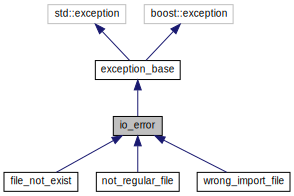
\includegraphics[width=350pt]{structio__error__inherit__graph}
\end{center}
\end{figure}


Collaboration diagram for io\+\_\+error\+:\nopagebreak
\begin{figure}[H]
\begin{center}
\leavevmode
\includegraphics[width=266pt]{structio__error__coll__graph}
\end{center}
\end{figure}


\subsection{Detailed Description}
struct defining the base of the \hyperlink{classIO}{I\+O} errors 

Definition at line 30 of file Exceptions.\+h.



The documentation for this class was generated from the following file\+:\begin{DoxyCompactItemize}
\item 
headers/\hyperlink{Exceptions_8h}{Exceptions.\+h}\end{DoxyCompactItemize}

\hypertarget{classMainWindow}{\section{Main\+Window Class Reference}
\label{classMainWindow}\index{Main\+Window@{Main\+Window}}
}


Builds the main window of the program extends Q\+Main\+Window.  




{\ttfamily \#include $<$Main\+Window.\+h$>$}



Inheritance diagram for Main\+Window\+:\nopagebreak
\begin{figure}[H]
\begin{center}
\leavevmode
\includegraphics[width=160pt]{classMainWindow__inherit__graph}
\end{center}
\end{figure}


Collaboration diagram for Main\+Window\+:\nopagebreak
\begin{figure}[H]
\begin{center}
\leavevmode
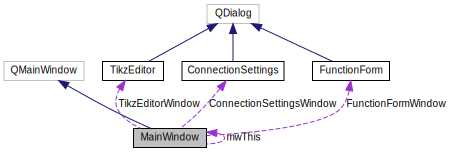
\includegraphics[width=350pt]{classMainWindow__coll__graph}
\end{center}
\end{figure}
\subsection*{Public Slots}
\begin{DoxyCompactItemize}
\item 
\hyperlink{classMyArea}{My\+Area} $\ast$ \hyperlink{classMainWindow_ad5bf28e8dd9343b4716b90ce2be83d64}{open\+Tab} ()
\begin{DoxyCompactList}\small\item\em opens a new tab \end{DoxyCompactList}\item 
\hypertarget{classMainWindow_a3ba1a371fb10e731ae0926ae85efeb4f}{void \hyperlink{classMainWindow_a3ba1a371fb10e731ae0926ae85efeb4f}{save} ()}\label{classMainWindow_a3ba1a371fb10e731ae0926ae85efeb4f}

\begin{DoxyCompactList}\small\item\em saves the file \end{DoxyCompactList}\item 
\hypertarget{classMainWindow_af622a541e4d87f86e9e83d29af60fe19}{void \hyperlink{classMainWindow_af622a541e4d87f86e9e83d29af60fe19}{close\+Tab} ()}\label{classMainWindow_af622a541e4d87f86e9e83d29af60fe19}

\begin{DoxyCompactList}\small\item\em closes the active tab \end{DoxyCompactList}\item 
\hypertarget{classMainWindow_a111875a1d82e77178636322ab485e4bb}{void \hyperlink{classMainWindow_a111875a1d82e77178636322ab485e4bb}{export\+Png} ()}\label{classMainWindow_a111875a1d82e77178636322ab485e4bb}

\begin{DoxyCompactList}\small\item\em exports the current view to P\+N\+G file \end{DoxyCompactList}\item 
\hypertarget{classMainWindow_a0423cda4bfa3846796523893e2deb5f1}{void \hyperlink{classMainWindow_a0423cda4bfa3846796523893e2deb5f1}{export\+Dot} ()}\label{classMainWindow_a0423cda4bfa3846796523893e2deb5f1}

\begin{DoxyCompactList}\small\item\em exports the current file to D\+O\+T file \end{DoxyCompactList}\item 
\hypertarget{classMainWindow_aafce9e112fde4466c72e1e49dd7c87e6}{void \hyperlink{classMainWindow_aafce9e112fde4466c72e1e49dd7c87e6}{open\+Editor} ()}\label{classMainWindow_aafce9e112fde4466c72e1e49dd7c87e6}

\begin{DoxyCompactList}\small\item\em open the editor before generating the tik\+Z file \end{DoxyCompactList}\item 
\hypertarget{classMainWindow_a6508549190bb7d638e48317c65ed7380}{void \hyperlink{classMainWindow_a6508549190bb7d638e48317c65ed7380}{export\+X\+M\+L\+Metadata} ()}\label{classMainWindow_a6508549190bb7d638e48317c65ed7380}

\begin{DoxyCompactList}\small\item\em exports style and layout data to X\+M\+L format \end{DoxyCompactList}\item 
\hypertarget{classMainWindow_aacfffa2dff97903be79cd39468ed0388}{void \hyperlink{classMainWindow_aacfffa2dff97903be79cd39468ed0388}{import\+X\+M\+L\+Metadata} (Q\+String temp\+X\+M\+L=\char`\"{}\char`\"{})}\label{classMainWindow_aacfffa2dff97903be79cd39468ed0388}

\begin{DoxyCompactList}\small\item\em imports style and layout data from X\+M\+L format \end{DoxyCompactList}\item 
\hypertarget{classMainWindow_a38a21fe3722b03dff23981f5e7a7fb50}{void \hyperlink{classMainWindow_a38a21fe3722b03dff23981f5e7a7fb50}{adjust} ()}\label{classMainWindow_a38a21fe3722b03dff23981f5e7a7fb50}

\begin{DoxyCompactList}\small\item\em fits the scale to see the entire window \end{DoxyCompactList}\item 
\hypertarget{classMainWindow_aa13e39ece777521d3f176155899309a6}{void \hyperlink{classMainWindow_aa13e39ece777521d3f176155899309a6}{zoom\+In} ()}\label{classMainWindow_aa13e39ece777521d3f176155899309a6}

\begin{DoxyCompactList}\small\item\em zooms the view in \end{DoxyCompactList}\item 
\hypertarget{classMainWindow_a21d4700dd4bc51216443a4c788b85892}{void \hyperlink{classMainWindow_a21d4700dd4bc51216443a4c788b85892}{zoom\+Out} ()}\label{classMainWindow_a21d4700dd4bc51216443a4c788b85892}

\begin{DoxyCompactList}\small\item\em zooms the view out \end{DoxyCompactList}\item 
\hypertarget{classMainWindow_a70de6a437bf79b2e94bfeb24e7207592}{void \hyperlink{classMainWindow_a70de6a437bf79b2e94bfeb24e7207592}{switch\+To\+Simplified\+Model} ()}\label{classMainWindow_a70de6a437bf79b2e94bfeb24e7207592}

\begin{DoxyCompactList}\small\item\em set all sorts of the scene into simplified model \end{DoxyCompactList}\item 
\hypertarget{classMainWindow_a08da9d2c3f6beb57e2172fe02fa08e6e}{void \hyperlink{classMainWindow_a08da9d2c3f6beb57e2172fe02fa08e6e}{switch\+To\+Detailled\+Model} ()}\label{classMainWindow_a08da9d2c3f6beb57e2172fe02fa08e6e}

\begin{DoxyCompactList}\small\item\em set all sorts of the scene into detailled model \end{DoxyCompactList}\item 
\hypertarget{classMainWindow_a1a7e2b9194e7134bca5fcf1dd4842a07}{void \hyperlink{classMainWindow_a1a7e2b9194e7134bca5fcf1dd4842a07}{change\+Background\+Color} ()}\label{classMainWindow_a1a7e2b9194e7134bca5fcf1dd4842a07}

\begin{DoxyCompactList}\small\item\em let the user set the background color \end{DoxyCompactList}\item 
\hypertarget{classMainWindow_a608f0b442dc8d0e1c68807b1955d5182}{void \hyperlink{classMainWindow_a608f0b442dc8d0e1c68807b1955d5182}{change\+Sort\+Color} ()}\label{classMainWindow_a608f0b442dc8d0e1c68807b1955d5182}

\begin{DoxyCompactList}\small\item\em let the user set the sorts color \end{DoxyCompactList}\item 
\hypertarget{classMainWindow_a53a978130fe29018994d68086887cec6}{void \hyperlink{classMainWindow_a53a978130fe29018994d68086887cec6}{positive\+Contrast} ()}\label{classMainWindow_a53a978130fe29018994d68086887cec6}

\begin{DoxyCompactList}\small\item\em sets default style\+: natural contrast (white background) \end{DoxyCompactList}\item 
\hypertarget{classMainWindow_af24af65044c4d11840848c7e88aee5ab}{void \hyperlink{classMainWindow_af24af65044c4d11840848c7e88aee5ab}{negative\+Contrast} ()}\label{classMainWindow_af24af65044c4d11840848c7e88aee5ab}

\begin{DoxyCompactList}\small\item\em sets default style\+: negative contrast (dark background) \end{DoxyCompactList}\item 
\hypertarget{classMainWindow_acff3aa2177db565ca2e2ced7a70ca46e}{void \hyperlink{classMainWindow_acff3aa2177db565ca2e2ced7a70ca46e}{print\+Style} ()}\label{classMainWindow_acff3aa2177db565ca2e2ced7a70ca46e}

\begin{DoxyCompactList}\small\item\em sets default style\+: compatible with print (empty sorts\+: \char`\"{}wired\char`\"{} style) \end{DoxyCompactList}\item 
\hypertarget{classMainWindow_ad76e17f0b71ff5e14addac21b81551b7}{void \hyperlink{classMainWindow_ad76e17f0b71ff5e14addac21b81551b7}{hide\+Show\+Text} ()}\label{classMainWindow_ad76e17f0b71ff5e14addac21b81551b7}

\begin{DoxyCompactList}\small\item\em hide / show the text area \end{DoxyCompactList}\item 
\hypertarget{classMainWindow_affc0ddbc2bff4b3fab7c95df8ec4322b}{void \hyperlink{classMainWindow_affc0ddbc2bff4b3fab7c95df8ec4322b}{change\+Text\+Background\+Color} ()}\label{classMainWindow_affc0ddbc2bff4b3fab7c95df8ec4322b}

\begin{DoxyCompactList}\small\item\em change text background color \end{DoxyCompactList}\item 
\hypertarget{classMainWindow_ad7f2cca8049e971e9e6cebfff35296e8}{void \hyperlink{classMainWindow_ad7f2cca8049e971e9e6cebfff35296e8}{hide\+Show\+Tree} ()}\label{classMainWindow_ad7f2cca8049e971e9e6cebfff35296e8}

\begin{DoxyCompactList}\small\item\em hide / show the tree area \end{DoxyCompactList}\item 
\hypertarget{classMainWindow_a879f655b0a921bc80bd316579e98c366}{void \hyperlink{classMainWindow_a879f655b0a921bc80bd316579e98c366}{find\+Fixpoints} ()}\label{classMainWindow_a879f655b0a921bc80bd316579e98c366}

\begin{DoxyCompactList}\small\item\em executes pint program\+: ph-\/stable \end{DoxyCompactList}\item 
\hypertarget{classMainWindow_a0c7fe8e75bbc5113df5e514214908ab3}{void \hyperlink{classMainWindow_a0c7fe8e75bbc5113df5e514214908ab3}{compute\+Reachability} ()}\label{classMainWindow_a0c7fe8e75bbc5113df5e514214908ab3}

\begin{DoxyCompactList}\small\item\em executes pint program\+: ph-\/reach \end{DoxyCompactList}\item 
\hypertarget{classMainWindow_ae9027bd9df095e7ed2f8bf28270e5d98}{void \hyperlink{classMainWindow_ae9027bd9df095e7ed2f8bf28270e5d98}{Edit\+Tikz\+Data} ()}\label{classMainWindow_ae9027bd9df095e7ed2f8bf28270e5d98}

\begin{DoxyCompactList}\small\item\em executes pint program\+: ph-\/reach \end{DoxyCompactList}\item 
\hypertarget{classMainWindow_ab8eeb1e902f4591fc2f35237a1faef01}{void \hyperlink{classMainWindow_ab8eeb1e902f4591fc2f35237a1faef01}{run\+Stochastic\+Simulation} ()}\label{classMainWindow_ab8eeb1e902f4591fc2f35237a1faef01}

\begin{DoxyCompactList}\small\item\em executes pint program\+: ph-\/exec \end{DoxyCompactList}\item 
\hypertarget{classMainWindow_ace4bc6f63b25822514dd2250bbb4760f}{void \hyperlink{classMainWindow_ace4bc6f63b25822514dd2250bbb4760f}{check\+Model\+Type} ()}\label{classMainWindow_ace4bc6f63b25822514dd2250bbb4760f}

\begin{DoxyCompactList}\small\item\em checks the type of the model \end{DoxyCompactList}\item 
\hypertarget{classMainWindow_a3eee76227ea883705553abe5e1f2a2be}{void \hyperlink{classMainWindow_a3eee76227ea883705553abe5e1f2a2be}{statistics} ()}\label{classMainWindow_a3eee76227ea883705553abe5e1f2a2be}

\begin{DoxyCompactList}\small\item\em calls ph-\/stat functionality of pint \end{DoxyCompactList}\item 
void \hyperlink{classMainWindow_a5f56ea1ee38eb16074e654b8bd52d072}{disable\+Menu} (Q\+Mdi\+Sub\+Window $\ast$sub\+Window)
\begin{DoxyCompactList}\small\item\em disables the menus that are related to open, active tabs \end{DoxyCompactList}\item 
\hypertarget{classMainWindow_a3fbd0b3e2fb9008ffa476d79a951d3dd}{void \hyperlink{classMainWindow_a3fbd0b3e2fb9008ffa476d79a951d3dd}{search\+Sort} ()}\label{classMainWindow_a3fbd0b3e2fb9008ffa476d79a951d3dd}

\begin{DoxyCompactList}\small\item\em search a sort in the \hyperlink{classSort}{Sort} Tree \end{DoxyCompactList}\item 
\hypertarget{classMainWindow_a74bc22370f5443cd3ca04be2cbeca061}{void \hyperlink{classMainWindow_a74bc22370f5443cd3ca04be2cbeca061}{open\+Connection} ()}\label{classMainWindow_a74bc22370f5443cd3ca04be2cbeca061}

\begin{DoxyCompactList}\small\item\em open connection settings window to implement a new function \end{DoxyCompactList}\item 
\hypertarget{classMainWindow_ab0df9fa0819262a27793630c19824b5b}{void {\bfseries open\+Connection\+Form} ()}\label{classMainWindow_ab0df9fa0819262a27793630c19824b5b}

\end{DoxyCompactItemize}
\subsection*{Public Member Functions}
\begin{DoxyCompactItemize}
\item 
\hypertarget{classMainWindow_ab4a9ef5dbbfabf44e6af7494287307aa}{Q\+String\+List {\bfseries word\+List} (const Q\+String \&text)}\label{classMainWindow_ab4a9ef5dbbfabf44e6af7494287307aa}

\item 
\hypertarget{classMainWindow_a34c4b4207b46d11a4100c9b19f0e81bb}{\hyperlink{classMainWindow_a34c4b4207b46d11a4100c9b19f0e81bb}{Main\+Window} ()}\label{classMainWindow_a34c4b4207b46d11a4100c9b19f0e81bb}

\begin{DoxyCompactList}\small\item\em constructor\+: creates the window, the menus and initializes the characteristics \end{DoxyCompactList}\item 
Q\+Mdi\+Area $\ast$ \hyperlink{classMainWindow_a7ef4a7c09626b415053b30bc412a3b1f}{get\+Centrale\+Area} ()
\begin{DoxyCompactList}\small\item\em gets centrale\+Area \end{DoxyCompactList}\item 
\hypertarget{classMainWindow_afabdfcfe9a925f3b91d93980da94068e}{std\+::vector$<$ Q\+String $>$ \hyperlink{classMainWindow_afabdfcfe9a925f3b91d93980da94068e}{get\+All\+Paths} ()}\label{classMainWindow_afabdfcfe9a925f3b91d93980da94068e}

\begin{DoxyCompactList}\small\item\em gets the paths of all the \hyperlink{classPH}{P\+H} files that are currently opened \end{DoxyCompactList}\item 
void \hyperlink{classMainWindow_a8a30572d7170d0a51737cd4991f0a05f}{compute} (Q\+String program, Q\+String\+List arguments, Q\+String file\+Name=\char`\"{}\char`\"{})
\begin{DoxyCompactList}\small\item\em calls the pint pr\+Connection\+Settings()ogram with the given arguments \end{DoxyCompactList}\item 
void \hyperlink{classMainWindow_ac4c3ec77ba5666ff9ef670b4b02c6838}{enable\+Menu} ()
\begin{DoxyCompactList}\small\item\em enables the menus that are related to any open, active tab \end{DoxyCompactList}\item 
\hypertarget{classMainWindow_a40c1a091a42559d7531ee79b6debd323}{Q\+String {\bfseries path\+Current\+Window} ()}\label{classMainWindow_a40c1a091a42559d7531ee79b6debd323}

\end{DoxyCompactItemize}
\subsection*{Static Public Attributes}
\begin{DoxyCompactItemize}
\item 
\hypertarget{classMainWindow_a3e20293fd9bb07ee5c220ac0b3b5991e}{static \hyperlink{classMainWindow}{Main\+Window} $\ast$ {\bfseries mw\+This}}\label{classMainWindow_a3e20293fd9bb07ee5c220ac0b3b5991e}

\end{DoxyCompactItemize}
\subsection*{Protected Attributes}
\begin{DoxyCompactItemize}
\item 
\hypertarget{classMainWindow_af5df9378db57a148236d639dd928d08f}{Q\+Mdi\+Area $\ast$ \hyperlink{classMainWindow_af5df9378db57a148236d639dd928d08f}{centrale\+Area}}\label{classMainWindow_af5df9378db57a148236d639dd928d08f}

\begin{DoxyCompactList}\small\item\em pointer to the central area of the window \end{DoxyCompactList}\item 
\hypertarget{classMainWindow_ab2049e45c3b990813bfba9e385cfa93a}{\hyperlink{classConnectionSettings}{Connection\+Settings} $\ast$ {\bfseries Connection\+Settings\+Window}}\label{classMainWindow_ab2049e45c3b990813bfba9e385cfa93a}

\item 
\hypertarget{classMainWindow_a79dcb4ded5b6e74882366b30132446ee}{\hyperlink{classFunctionForm}{Function\+Form} $\ast$ {\bfseries Function\+Form\+Window}}\label{classMainWindow_a79dcb4ded5b6e74882366b30132446ee}

\item 
\hypertarget{classMainWindow_a489592ba062ec5f7eafb408fdc184322}{\hyperlink{classTikzEditor}{Tikz\+Editor} $\ast$ {\bfseries Tikz\+Editor\+Window}}\label{classMainWindow_a489592ba062ec5f7eafb408fdc184322}

\item 
\hypertarget{classMainWindow_a2ca04227e7d71b036ccd0ed4176a5561}{Q\+Menu $\ast$ {\bfseries menu\+File}}\label{classMainWindow_a2ca04227e7d71b036ccd0ed4176a5561}

\item 
\hypertarget{classMainWindow_a51ec7fcfcb60073b395dee46daacf1f9}{Q\+Menu $\ast$ {\bfseries menu\+Edit}}\label{classMainWindow_a51ec7fcfcb60073b395dee46daacf1f9}

\item 
\hypertarget{classMainWindow_a57793b17cc2b8de42b5b10e9458ae9cb}{Q\+Menu $\ast$ {\bfseries menu\+View}}\label{classMainWindow_a57793b17cc2b8de42b5b10e9458ae9cb}

\item 
\hypertarget{classMainWindow_a559074b0cbdcb3183a201b105cc81610}{Q\+Menu $\ast$ {\bfseries menu\+Styles}}\label{classMainWindow_a559074b0cbdcb3183a201b105cc81610}

\item 
\hypertarget{classMainWindow_a2ddd0dbbad4b426293bc9480075b8a56}{Q\+Menu $\ast$ {\bfseries menu\+Window}}\label{classMainWindow_a2ddd0dbbad4b426293bc9480075b8a56}

\item 
\hypertarget{classMainWindow_a8142152915924723cee2f22e0868a852}{Q\+Menu $\ast$ {\bfseries menu\+Computation}}\label{classMainWindow_a8142152915924723cee2f22e0868a852}

\item 
\hypertarget{classMainWindow_a81d80bba8e8a31cea2bb218094890c81}{Q\+Menu $\ast$ {\bfseries menu\+Help}}\label{classMainWindow_a81d80bba8e8a31cea2bb218094890c81}

\item 
\hypertarget{classMainWindow_afcc4de380e40fe4aeb61b07402f00f58}{Q\+Action $\ast$ {\bfseries action\+New}}\label{classMainWindow_afcc4de380e40fe4aeb61b07402f00f58}

\item 
\hypertarget{classMainWindow_ab5342d85523e2dad5b6f69a6ad01ece3}{Q\+Action $\ast$ {\bfseries action\+Open}}\label{classMainWindow_ab5342d85523e2dad5b6f69a6ad01ece3}

\item 
\hypertarget{classMainWindow_ac785bdaae348156fc94fdfea23f67a90}{Q\+Action $\ast$ {\bfseries action\+Saveas}}\label{classMainWindow_ac785bdaae348156fc94fdfea23f67a90}

\item 
\hypertarget{classMainWindow_a509ebce4344493751dec180d55d3b107}{Q\+Menu $\ast$ {\bfseries menu\+Export}}\label{classMainWindow_a509ebce4344493751dec180d55d3b107}

\item 
\hypertarget{classMainWindow_a233dc8b191a12c682366d27a3d9e568f}{Q\+Action $\ast$ {\bfseries action\+Png}}\label{classMainWindow_a233dc8b191a12c682366d27a3d9e568f}

\item 
\hypertarget{classMainWindow_a4bdcf20fae10e3adc9617e45217331eb}{Q\+Action $\ast$ {\bfseries action\+Dot}}\label{classMainWindow_a4bdcf20fae10e3adc9617e45217331eb}

\item 
\hypertarget{classMainWindow_a90b44b33ad276818e33cc917949b37fa}{Q\+Action $\ast$ {\bfseries action\+Export\+Tikz\+Data}}\label{classMainWindow_a90b44b33ad276818e33cc917949b37fa}

\item 
\hypertarget{classMainWindow_a25f11f87c05e1647a30602a1ab7788c0}{Q\+Action $\ast$ {\bfseries action\+Export\+X\+M\+L\+Data}}\label{classMainWindow_a25f11f87c05e1647a30602a1ab7788c0}

\item 
\hypertarget{classMainWindow_ad6346d52a17672595d9e7f9b8c531623}{Q\+Menu $\ast$ {\bfseries menu\+Import}}\label{classMainWindow_ad6346d52a17672595d9e7f9b8c531623}

\item 
\hypertarget{classMainWindow_aff4c14fea63a9f30d2fe03075c44e122}{Q\+Action $\ast$ {\bfseries action\+Forimport}}\label{classMainWindow_aff4c14fea63a9f30d2fe03075c44e122}

\item 
\hypertarget{classMainWindow_acf4206ba3c373585ad33ef09e0c8ccb3}{Q\+Action $\ast$ {\bfseries action\+Close}}\label{classMainWindow_acf4206ba3c373585ad33ef09e0c8ccb3}

\item 
\hypertarget{classMainWindow_a60f400ff0f2b281499611c5e0018d901}{Q\+Action $\ast$ {\bfseries action\+Quit}}\label{classMainWindow_a60f400ff0f2b281499611c5e0018d901}

\item 
\hypertarget{classMainWindow_aca6e412c6008053d39c5fbaf5133274b}{Q\+Action $\ast$ {\bfseries action\+Undo}}\label{classMainWindow_aca6e412c6008053d39c5fbaf5133274b}

\item 
\hypertarget{classMainWindow_aa1ea7fe519e373af34ba4f7669df14cd}{Q\+Action $\ast$ {\bfseries action\+Redo}}\label{classMainWindow_aa1ea7fe519e373af34ba4f7669df14cd}

\item 
\hypertarget{classMainWindow_a29f96f7f06943080dde36c4cbb243005}{Q\+Action $\ast$ {\bfseries action\+Simplified\+Model}}\label{classMainWindow_a29f96f7f06943080dde36c4cbb243005}

\item 
\hypertarget{classMainWindow_a1ab7437b6cfdd3aa2ef1e513a7703d6f}{Q\+Action $\ast$ {\bfseries action\+Detailled\+Model}}\label{classMainWindow_a1ab7437b6cfdd3aa2ef1e513a7703d6f}

\item 
\hypertarget{classMainWindow_a74a2eadbd881ef8b2e292a2964ff6f05}{Q\+Action $\ast$ {\bfseries action\+Adjust}}\label{classMainWindow_a74a2eadbd881ef8b2e292a2964ff6f05}

\item 
\hypertarget{classMainWindow_a2679c07380a989d6df6868664f4491dc}{Q\+Action $\ast$ {\bfseries action\+Zoom\+In}}\label{classMainWindow_a2679c07380a989d6df6868664f4491dc}

\item 
\hypertarget{classMainWindow_a6acc21e45e1bffd8b87c90000ed8542e}{Q\+Action $\ast$ {\bfseries action\+Zoom\+Out}}\label{classMainWindow_a6acc21e45e1bffd8b87c90000ed8542e}

\item 
\hypertarget{classMainWindow_a1149df8ffebf08ca08bafcef304a207a}{Q\+Action $\ast$ {\bfseries action\+Show\+Init}}\label{classMainWindow_a1149df8ffebf08ca08bafcef304a207a}

\item 
\hypertarget{classMainWindow_aab91a08cf5e63146ac25d266699344f7}{Q\+Action $\ast$ {\bfseries action\+Highlight}}\label{classMainWindow_aab91a08cf5e63146ac25d266699344f7}

\item 
\hypertarget{classMainWindow_a8d65feefc7d6d3d809b2466be1b6c176}{Q\+Action $\ast$ {\bfseries action\+Hide}}\label{classMainWindow_a8d65feefc7d6d3d809b2466be1b6c176}

\item 
\hypertarget{classMainWindow_afea5009cf5a1589c7921992310620c3f}{Q\+Action $\ast$ {\bfseries action\+Display\+Detailed}}\label{classMainWindow_afea5009cf5a1589c7921992310620c3f}

\item 
\hypertarget{classMainWindow_a470562bf456714b6f85b9534e4b6eef0}{Q\+Action $\ast$ {\bfseries action\+Background\+Color}}\label{classMainWindow_a470562bf456714b6f85b9534e4b6eef0}

\item 
\hypertarget{classMainWindow_ae24a527be55420779bce80763710e867}{Q\+Action $\ast$ {\bfseries action\+Sort\+Color}}\label{classMainWindow_ae24a527be55420779bce80763710e867}

\item 
\hypertarget{classMainWindow_a2f153d9eb2b29762d1d564de27fc7c43}{Q\+Menu $\ast$ {\bfseries menu\+Default\+Styles}}\label{classMainWindow_a2f153d9eb2b29762d1d564de27fc7c43}

\item 
\hypertarget{classMainWindow_ae3fc5a85c38fbeb92fbfe508c1f791fa}{Q\+Action $\ast$ {\bfseries action\+Natural\+Style}}\label{classMainWindow_ae3fc5a85c38fbeb92fbfe508c1f791fa}

\item 
\hypertarget{classMainWindow_a626146e0315df36a9d0c1afc73c4b8a9}{Q\+Action $\ast$ {\bfseries action\+Negative\+Style}}\label{classMainWindow_a626146e0315df36a9d0c1afc73c4b8a9}

\item 
\hypertarget{classMainWindow_a9f939857be21b16cab10fba41ff0e242}{Q\+Action $\ast$ {\bfseries action\+Print\+Style}}\label{classMainWindow_a9f939857be21b16cab10fba41ff0e242}

\item 
\hypertarget{classMainWindow_a606eaf5ca6bb26e0f4fdd5eb8aa84c58}{Q\+Menu $\ast$ {\bfseries menu\+Text}}\label{classMainWindow_a606eaf5ca6bb26e0f4fdd5eb8aa84c58}

\item 
\hypertarget{classMainWindow_a9b47436992df37538bc31e2d4d8ee067}{Q\+Action $\ast$ {\bfseries action\+Hide\+Show\+Text}}\label{classMainWindow_a9b47436992df37538bc31e2d4d8ee067}

\item 
\hypertarget{classMainWindow_a942f0384b4c4185504c810f5104faebc}{Q\+Action $\ast$ {\bfseries action\+Change\+Text\+Background\+Color}}\label{classMainWindow_a942f0384b4c4185504c810f5104faebc}

\item 
\hypertarget{classMainWindow_a0eebe45643eed419e08ddb8bd8da2a57}{Q\+Menu $\ast$ {\bfseries menu\+Tree}}\label{classMainWindow_a0eebe45643eed419e08ddb8bd8da2a57}

\item 
\hypertarget{classMainWindow_aca06fa2f83fb7500cc11543768067ae2}{Q\+Action $\ast$ {\bfseries action\+Hide\+Show\+Tree}}\label{classMainWindow_aca06fa2f83fb7500cc11543768067ae2}

\item 
\hypertarget{classMainWindow_a04048deb025090490f7261002a4ea4ab}{Q\+Action $\ast$ {\bfseries action\+Find\+Fixpoints}}\label{classMainWindow_a04048deb025090490f7261002a4ea4ab}

\item 
\hypertarget{classMainWindow_a2d5f7f2433aab9c8005c197bc96cdbc9}{Q\+Action $\ast$ {\bfseries action\+Compute\+Reachability}}\label{classMainWindow_a2d5f7f2433aab9c8005c197bc96cdbc9}

\item 
\hypertarget{classMainWindow_ae1ed3e80e7e9dc6e0687729e68071c37}{Q\+Action $\ast$ {\bfseries action\+Run\+Stochastic\+Simulation}}\label{classMainWindow_ae1ed3e80e7e9dc6e0687729e68071c37}

\item 
\hypertarget{classMainWindow_ab44ca117cab372eb7baea30cf0a6c8b0}{Q\+Action $\ast$ {\bfseries action\+Check\+Model\+Type}}\label{classMainWindow_ab44ca117cab372eb7baea30cf0a6c8b0}

\item 
\hypertarget{classMainWindow_ab81ef1d7f2f2dfc26b8ca9b50391692d}{Q\+Action $\ast$ {\bfseries action\+Statistics}}\label{classMainWindow_ab81ef1d7f2f2dfc26b8ca9b50391692d}

\item 
\hypertarget{classMainWindow_aafa2d178ba771586e76e391ca720ef08}{Q\+Menu $\ast$ {\bfseries menu\+Connection}}\label{classMainWindow_aafa2d178ba771586e76e391ca720ef08}

\item 
\hypertarget{classMainWindow_a07a7a6a4c296875a10ae54a91ff80584}{Q\+Action $\ast$ {\bfseries action\+Connection}}\label{classMainWindow_a07a7a6a4c296875a10ae54a91ff80584}

\item 
\hypertarget{classMainWindow_a09f3577bd1805791f47e506fa918d87c}{Q\+Action $\ast$ {\bfseries action\+New\+Connection}}\label{classMainWindow_a09f3577bd1805791f47e506fa918d87c}

\item 
\hypertarget{classMainWindow_aa533eee89cb4ec348b3df9c25f10f47f}{Q\+Action $\ast$ {\bfseries action\+Help}}\label{classMainWindow_aa533eee89cb4ec348b3df9c25f10f47f}

\end{DoxyCompactItemize}


\subsection{Detailed Description}
Builds the main window of the program extends Q\+Main\+Window. 

Definition at line 26 of file Main\+Window.\+h.



\subsection{Member Function Documentation}
\hypertarget{classMainWindow_a8a30572d7170d0a51737cd4991f0a05f}{\index{Main\+Window@{Main\+Window}!compute@{compute}}
\index{compute@{compute}!Main\+Window@{Main\+Window}}
\subsubsection[{compute}]{\setlength{\rightskip}{0pt plus 5cm}void Main\+Window\+::compute (
\begin{DoxyParamCaption}
\item[{Q\+String}]{program, }
\item[{Q\+String\+List}]{arguments, }
\item[{Q\+String}]{file\+Name = {\ttfamily \char`\"{}\char`\"{}}}
\end{DoxyParamCaption}
)}}\label{classMainWindow_a8a30572d7170d0a51737cd4991f0a05f}


calls the pint pr\+Connection\+Settings()ogram with the given arguments 


\begin{DoxyParams}{Parameters}
{\em Qstring} & the program to execute \\
\hline
{\em Q\+String\+List} & the arguments to give to the program \\
\hline
{\em Q\+String} & (optional) the name of the \hyperlink{classPH}{P\+H} file to parse \\
\hline
\end{DoxyParams}


Definition at line 1032 of file Main\+Window.\+cpp.


\begin{DoxyCode}
1032                                                                                  \{
1033 
1034     \textcolor{comment}{// start process}
1035     QProcess *myProcess = \textcolor{keyword}{new} QProcess();
1036 
1037     myProcess->start(program, arguments);
1038 
1039     \textcolor{keywordflow}{if} (!myProcess->waitForStarted())
1040         \textcolor{keywordflow}{throw} \hyperlink{structpint__program__not__found}{pint\_program\_not\_found}() << file\_info(\textcolor{stringliteral}{"phc"});
1041 
1042     \textcolor{comment}{// read result}
1043     QByteArray err;
1044     QByteArray out;
1045     \textcolor{keywordflow}{while} (!myProcess->waitForFinished()) \{
1046         err += myProcess->readAllStandardError();
1047         out += myProcess->readAllStandardOutput();
1048     \}
1049     err += myProcess->readAllStandardError();
1050     out += myProcess->readAllStandardOutput();
1051     \textcolor{keyword}{delete} myProcess;
1052 
1053     \textcolor{comment}{// pop up for the errors}
1054     \textcolor{keywordflow}{if}(!err.isEmpty()) \{
1055 
1056         \textcolor{comment}{//correct a false error message for ph-stable}
1057         \textcolor{keywordflow}{if}(program==QString(\textcolor{stringliteral}{"ph-stable"})) \{
1058             \textcolor{keywordflow}{if}( !(QString(err).contains(fileName)) || fileName.isEmpty() ) \{
1059                 QMessageBox::critical(\textcolor{keyword}{this}, program+\textcolor{stringliteral}{".error"}, err);
1060             \}
1061         \} \textcolor{keywordflow}{else} \{
1062             \textcolor{comment}{//correct a false error message for ph-exec}
1063             \textcolor{keywordflow}{if}(program!=QString(\textcolor{stringliteral}{"ph-exec"})) \{
1064                 QMessageBox::critical(\textcolor{keyword}{this}, program+\textcolor{stringliteral}{".error"}, err);
1065             \}
1066         \}
1067     \}
1068 
1069     \textcolor{comment}{//pop up for the output}
1070     \textcolor{keywordflow}{if}(!out.isEmpty()) \{
1071 
1072         QMessageBox::information(\textcolor{keyword}{this}, program+\textcolor{stringliteral}{".output"}, out);
1073 
1074     \}
1075 
1076 
1077 \}
\end{DoxyCode}
\hypertarget{classMainWindow_a5f56ea1ee38eb16074e654b8bd52d072}{\index{Main\+Window@{Main\+Window}!disable\+Menu@{disable\+Menu}}
\index{disable\+Menu@{disable\+Menu}!Main\+Window@{Main\+Window}}
\subsubsection[{disable\+Menu}]{\setlength{\rightskip}{0pt plus 5cm}void Main\+Window\+::disable\+Menu (
\begin{DoxyParamCaption}
\item[{Q\+Mdi\+Sub\+Window $\ast$}]{sub\+Window}
\end{DoxyParamCaption}
)\hspace{0.3cm}{\ttfamily [slot]}}}\label{classMainWindow_a5f56ea1ee38eb16074e654b8bd52d072}


disables the menus that are related to open, active tabs 


\begin{DoxyParams}{Parameters}
{\em Q\+Mdi\+Sub\+Window$\ast$} & menu you want to disable \\
\hline
\end{DoxyParams}


Definition at line 1262 of file Main\+Window.\+cpp.


\begin{DoxyCode}
1262                                                      \{
1263     \textcolor{keywordflow}{if}(subwindow==0&&this->\hyperlink{classMainWindow_a7ef4a7c09626b415053b30bc412a3b1f}{getCentraleArea}()->subWindowList().isEmpty()) \{
1264         this->actionClose->setEnabled(\textcolor{keyword}{false});
1265         this->actionSaveas->setEnabled(\textcolor{keyword}{false});
1266         this->actionPng->setEnabled(\textcolor{keyword}{false});
1267         this->actionDot->setEnabled(\textcolor{keyword}{false});
1268         this->actionExportXMLData->setEnabled(\textcolor{keyword}{false});
1269         \textcolor{comment}{//change to false after that}
1270         this->actionExportTikzData->setEnabled(\textcolor{keyword}{true});
1271         this->actionForimport->setEnabled(\textcolor{keyword}{false});
1272         this->actionAdjust->setEnabled(\textcolor{keyword}{false});
1273         this->actionZoomIn->setEnabled(\textcolor{keyword}{false});
1274         this->actionZoomOut->setEnabled(\textcolor{keyword}{false});
1275         this->actionSimplifiedModel->setEnabled(\textcolor{keyword}{false});
1276         this->actionDetailledModel->setEnabled(\textcolor{keyword}{false});
1277         this->actionBackgroundColor->setEnabled(\textcolor{keyword}{false});
1278         this->actionSortColor->setEnabled(\textcolor{keyword}{false});
1279         this->actionNaturalStyle->setEnabled(\textcolor{keyword}{false});
1280         this->actionNegativeStyle->setEnabled(\textcolor{keyword}{false});
1281         this->actionPrintStyle->setEnabled(\textcolor{keyword}{false});
1282         this->actionHideShowText->setEnabled(\textcolor{keyword}{false});
1283         this->actionChangeTextBackgroundColor->setEnabled(\textcolor{keyword}{false});
1284         this->actionHideShowTree->setEnabled(\textcolor{keyword}{false});
1285         this->actionFindFixpoints->setEnabled(\textcolor{keyword}{false});
1286         this->actionComputeReachability->setEnabled(\textcolor{keyword}{false});
1287         this->actionRunStochasticSimulation->setEnabled(\textcolor{keyword}{false});
1288         this->actionStatistics->setEnabled(\textcolor{keyword}{false});
1289         this->actionConnection->setEnabled(\textcolor{keyword}{false});
1290     \}
1291 \}
\end{DoxyCode}
\hypertarget{classMainWindow_ac4c3ec77ba5666ff9ef670b4b02c6838}{\index{Main\+Window@{Main\+Window}!enable\+Menu@{enable\+Menu}}
\index{enable\+Menu@{enable\+Menu}!Main\+Window@{Main\+Window}}
\subsubsection[{enable\+Menu}]{\setlength{\rightskip}{0pt plus 5cm}void Main\+Window\+::enable\+Menu (
\begin{DoxyParamCaption}
{}
\end{DoxyParamCaption}
)}}\label{classMainWindow_ac4c3ec77ba5666ff9ef670b4b02c6838}


enables the menus that are related to any open, active tab 

\begin{DoxyNote}{Note}
to be updated for each new feature of the application 
\end{DoxyNote}


Definition at line 1295 of file Main\+Window.\+cpp.


\begin{DoxyCode}
1295                             \{
1296     \textcolor{keywordflow}{if}(!this->\hyperlink{classMainWindow_a7ef4a7c09626b415053b30bc412a3b1f}{getCentraleArea}()->subWindowList().isEmpty()) \{
1297         this->actionClose->setEnabled(\textcolor{keyword}{true});
1298         this->actionSaveas->setEnabled(\textcolor{keyword}{true});
1299         this->actionPng->setEnabled(\textcolor{keyword}{true});
1300         this->actionDot->setEnabled(\textcolor{keyword}{true});
1301         this->actionExportXMLData->setEnabled(\textcolor{keyword}{true});
1302         this->actionExportTikzData->setEnabled(\textcolor{keyword}{true});
1303         this->actionForimport->setEnabled(\textcolor{keyword}{true});
1304         this->actionAdjust->setEnabled(\textcolor{keyword}{true});
1305         this->actionZoomIn->setEnabled(\textcolor{keyword}{true});
1306         this->actionZoomOut->setEnabled(\textcolor{keyword}{true});
1307         this->actionSimplifiedModel->setEnabled(\textcolor{keyword}{true});
1308         this->actionDetailledModel->setEnabled(\textcolor{keyword}{true});
1309         this->actionBackgroundColor->setEnabled(\textcolor{keyword}{true});
1310         this->actionSortColor->setEnabled(\textcolor{keyword}{true});
1311         this->actionNaturalStyle->setEnabled(\textcolor{keyword}{true});
1312         this->actionNegativeStyle->setEnabled(\textcolor{keyword}{true});
1313         this->actionPrintStyle->setEnabled(\textcolor{keyword}{true});
1314         this->actionHideShowText->setEnabled(\textcolor{keyword}{true});
1315         this->actionChangeTextBackgroundColor->setEnabled(\textcolor{keyword}{true});
1316         this->actionHideShowTree->setEnabled(\textcolor{keyword}{true});
1317         this->actionFindFixpoints->setEnabled(\textcolor{keyword}{true});
1318         this->actionComputeReachability->setEnabled(\textcolor{keyword}{true});
1319         this->actionRunStochasticSimulation->setEnabled(\textcolor{keyword}{true});
1320         this->actionStatistics->setEnabled(\textcolor{keyword}{true});
1321 
1322         \textcolor{keywordflow}{if}(ConnectionSettings::tabFunction.size()!=0) \{
1323 
1324             this->actionConnection->setEnabled(\textcolor{keyword}{true});
1325         \}
1326     \}
1327 \}
\end{DoxyCode}
\hypertarget{classMainWindow_a7ef4a7c09626b415053b30bc412a3b1f}{\index{Main\+Window@{Main\+Window}!get\+Centrale\+Area@{get\+Centrale\+Area}}
\index{get\+Centrale\+Area@{get\+Centrale\+Area}!Main\+Window@{Main\+Window}}
\subsubsection[{get\+Centrale\+Area}]{\setlength{\rightskip}{0pt plus 5cm}Q\+Mdi\+Area $\ast$ Main\+Window\+::get\+Centrale\+Area (
\begin{DoxyParamCaption}
{}
\end{DoxyParamCaption}
)}}\label{classMainWindow_a7ef4a7c09626b415053b30bc412a3b1f}


gets centrale\+Area 

\begin{DoxyReturn}{Returns}
Q\+Mdi\+Area$\ast$ pointer to the central zone of the window 
\end{DoxyReturn}


Definition at line 233 of file Main\+Window.\+cpp.


\begin{DoxyCode}
233                                       \{
234     \textcolor{keywordflow}{return} this->\hyperlink{classMainWindow_af5df9378db57a148236d639dd928d08f}{centraleArea};
235 \}
\end{DoxyCode}
\hypertarget{classMainWindow_ad5bf28e8dd9343b4716b90ce2be83d64}{\index{Main\+Window@{Main\+Window}!open\+Tab@{open\+Tab}}
\index{open\+Tab@{open\+Tab}!Main\+Window@{Main\+Window}}
\subsubsection[{open\+Tab}]{\setlength{\rightskip}{0pt plus 5cm}{\bf My\+Area} $\ast$ Main\+Window\+::open\+Tab (
\begin{DoxyParamCaption}
{}
\end{DoxyParamCaption}
)\hspace{0.3cm}{\ttfamily [slot]}}}\label{classMainWindow_ad5bf28e8dd9343b4716b90ce2be83d64}


opens a new tab 

\begin{DoxyReturn}{Returns}
My\+Area$\ast$ pointer to newly created \hyperlink{classMyArea}{My\+Area} object 
\end{DoxyReturn}


Definition at line 252 of file Main\+Window.\+cpp.


\begin{DoxyCode}
252                             \{
253 
254     \textcolor{comment}{// OpenFile dialog}
255     QFileDialog* filedialog = \textcolor{keyword}{new} QFileDialog(\textcolor{keyword}{this});
256 
257     QDialog* mb = \textcolor{keyword}{new} QDialog(filedialog);
258     mb->setFixedSize(300,150);
259     mb->setWindowFlags(Qt::Window | Qt::WindowTitleHint | Qt::CustomizeWindowHint);
260 
261     QString file = filedialog->getOpenFileName(\textcolor{keyword}{this}, \textcolor{stringliteral}{"Open..."});
262 
263     \textcolor{comment}{// TODO refactor using early returns}
264     \textcolor{keywordflow}{if}(file!=NULL) \{
265         \textcolor{comment}{// Initiates timeopening calculation}
266         std::ofstream logFile(\textcolor{stringliteral}{"log\_opening\_time.txt"},std::ios::app);
267         std::chrono::steady\_clock::time\_point depart, arrivee;
268         depart = std::chrono::steady\_clock::now();
269         QFileInfo pathInfo(file);
270         std::vector<QString> allPath = this->\hyperlink{classMainWindow_afabdfcfe9a925f3b91d93980da94068e}{getAllPaths}();
271         \textcolor{keywordtype}{int} size = allPath.size();
272         \textcolor{keywordtype}{bool} alreadyOpen = \textcolor{keyword}{false};
273 
274         \textcolor{comment}{// check if the file is already open}
275         \textcolor{keywordflow}{for}(\textcolor{keywordtype}{int} i=0; i<size; i++) \{
276             \textcolor{keywordflow}{if}(allPath[i]==file) \{
277                 alreadyOpen = \textcolor{keyword}{true};
278                 \textcolor{keywordflow}{break};
279             \}
280         \}
281 
282 
283         \textcolor{keywordflow}{if}(!alreadyOpen) \{
284 
285             \textcolor{comment}{//Display loading window}
286             QLabel* dialogue = \textcolor{keyword}{new} QLabel(mb);
287             mb->setWindowTitle(\textcolor{stringliteral}{"Please wait..."});
288             QMovie* gif = \textcolor{keyword}{new} QMovie(\textcolor{stringliteral}{"loading.gif"});
289             gif->setScaledSize(QSize(300,150));
290             gif->start();
291             dialogue->setMovie(gif);
292             dialogue->show();
293             mb->open();
294 
295             \textcolor{comment}{//need a std::string instead of a QString}
296             std::string path =  file.toStdString();
297 
298             \textcolor{comment}{// parse file}
299             \hyperlink{classArea}{Area} *area = \textcolor{keyword}{new} \hyperlink{classArea}{Area}(\textcolor{keyword}{this}, QString::fromStdString(path));
300             area->\hyperlink{classArea_a78dfb0c8316dbe90af1e5c905db5b6d1}{mainWindow} = \textcolor{keyword}{this};
301 
302             \textcolor{keywordflow}{try} \{
303                 \textcolor{comment}{// render graph}
304                 PHPtr myPHPtr = \hyperlink{classPHIO_a392414cadc400154232f5488fba80600}{PHIO::parseFile}(path);
305                 area->\hyperlink{classArea_a3c00ea9bb14425efbee3fcf80410c4cf}{myArea}->\hyperlink{classMyArea_a087c389370070a348af025aaee620fc8}{setPHPtr}(myPHPtr);
306                 myPHPtr->render();
307                 PHScenePtr scene = myPHPtr->getGraphicsScene();
308                 area->\hyperlink{classArea_a3c00ea9bb14425efbee3fcf80410c4cf}{myArea}->setScene(&*scene);
309 
310                 \textcolor{comment}{// set the pointer of the treeArea}
311                 area->\hyperlink{classArea_a950b6ed9a4e754ef1a7879b727ea8749}{treeArea}->\hyperlink{classTreeArea_a290d659da16085f21c04f81fcd16891c}{myPHPtr} = myPHPtr;
312                 \textcolor{comment}{//set the pointer of the treeArea}
313                 area->\hyperlink{classArea_a950b6ed9a4e754ef1a7879b727ea8749}{treeArea}->\hyperlink{classTreeArea_a1bd090dc9ab10415e8f897b6300bc555}{myArea} = area->\hyperlink{classArea_a3c00ea9bb14425efbee3fcf80410c4cf}{myArea};
314                 \textcolor{comment}{// build the tree in the treeArea}
315                 area->\hyperlink{classArea_a950b6ed9a4e754ef1a7879b727ea8749}{treeArea}->\hyperlink{classTreeArea_a8fd7c22b1c8c4e8cb9503731d66c5d47}{build}();
316 
317                 \textcolor{comment}{// call the PH file and write it in the text area (same as .ph)}
318                 QFile fichier(file);
319                 fichier.open(QIODevice::ReadOnly);
320                 QByteArray data;
321                 data = fichier.readAll();
322                 QString ligne(data);
323                 area->\hyperlink{classArea_a001e5b841c3e4126a128de13171f05d3}{textArea}->setPlainText(ligne);
324 
325                 \textcolor{comment}{// make the subwindow for the new tab}
326                 QMdiSubWindow *theNewTab = this->\hyperlink{classMainWindow_a7ef4a7c09626b415053b30bc412a3b1f}{getCentraleArea}()->addSubWindow(area);
327                 QString fileName(pathInfo.fileName());
328                 theNewTab->setWindowTitle(fileName);
329                 this->\hyperlink{classMainWindow_ac4c3ec77ba5666ff9ef670b4b02c6838}{enableMenu}();
330 
331                 mb->close();
332                 this->setWindowState(Qt::WindowMaximized);
333                 \textcolor{comment}{// putting time needed to open ph file into a "log\_opening\_time.txt" file}
334                 arrivee = std::chrono::steady\_clock::now();
335                 \textcolor{keyword}{auto} timeOpening =
336                     std::chrono::duration\_cast<std::chrono::milliseconds>
337                         (arrivee - depart)
338                     .count();
339                 logFile << file.toStdString()+\textcolor{stringliteral}{"-----"}+\textcolor{stringliteral}{"-----"} << timeOpening;
340                 logFile << \textcolor{stringliteral}{" ms\(\backslash\)n"};
341                 logFile.close();
342                 \textcolor{keywordflow}{return} area->\hyperlink{classArea_a3c00ea9bb14425efbee3fcf80410c4cf}{myArea};
343 
344             \} \textcolor{keywordflow}{catch}(\hyperlink{structexception__base}{exception\_base}& argh) \{
345                 mb->close();
346                 QMessageBox::critical(\textcolor{keyword}{this}, \textcolor{stringliteral}{"Error"}, \textcolor{stringliteral}{"Extension not recognized. Only ph files are accepted.
      "});
347                 \textcolor{keywordflow}{return} NULL;
348             \}
349         \} \textcolor{keywordflow}{else} \{
350             mb->close();
351             QMessageBox::critical(\textcolor{keyword}{this}, \textcolor{stringliteral}{"Error"}, \textcolor{stringliteral}{"This file is already opened!"});
352             \textcolor{keywordflow}{return} NULL;
353         \}
354 
355 
356 
357     \} \textcolor{keywordflow}{else} \{
358         mb->close();
359         \textcolor{keywordflow}{return} NULL;
360     \}
361 \}
\end{DoxyCode}


The documentation for this class was generated from the following files\+:\begin{DoxyCompactItemize}
\item 
headers/\hyperlink{MainWindow_8h}{Main\+Window.\+h}\item 
src/ui/Main\+Window.\+cpp\end{DoxyCompactItemize}

\hypertarget{classMyArea}{\section{My\+Area Class Reference}
\label{classMyArea}\index{My\+Area@{My\+Area}}
}


Graph Widget extends Q\+Graphics\+View.  




{\ttfamily \#include $<$My\+Area.\+h$>$}



Inheritance diagram for My\+Area\+:\nopagebreak
\begin{figure}[H]
\begin{center}
\leavevmode
\includegraphics[width=165pt]{classMyArea__inherit__graph}
\end{center}
\end{figure}


Collaboration diagram for My\+Area\+:\nopagebreak
\begin{figure}[H]
\begin{center}
\leavevmode
\includegraphics[width=165pt]{classMyArea__coll__graph}
\end{center}
\end{figure}
\subsection*{Public Member Functions}
\begin{DoxyCompactItemize}
\item 
\hyperlink{classMyArea_a31f13e95c83414c538b6c46e55e19c79}{My\+Area} (Q\+String \hyperlink{classMyArea_a70561a408470de740f580da6717871bf}{path})
\begin{DoxyCompactList}\small\item\em constructor \end{DoxyCompactList}\item 
\hyperlink{classMyArea_af3c945c22987982a37dc47dad0c24615}{My\+Area} (Q\+Widget $\ast$parent, Q\+String \hyperlink{classMyArea_a70561a408470de740f580da6717871bf}{path})
\begin{DoxyCompactList}\small\item\em constructor \end{DoxyCompactList}\item 
\hypertarget{classMyArea_a7b94b516e730ddcee16d946c76bbc2b3}{P\+H\+Ptr \hyperlink{classMyArea_a7b94b516e730ddcee16d946c76bbc2b3}{get\+P\+H\+Ptr} ()}\label{classMyArea_a7b94b516e730ddcee16d946c76bbc2b3}

\begin{DoxyCompactList}\small\item\em gets my\+P\+H\+Ptr \end{DoxyCompactList}\item 
\hypertarget{classMyArea_a087c389370070a348af025aaee620fc8}{void \hyperlink{classMyArea_a087c389370070a348af025aaee620fc8}{set\+P\+H\+Ptr} (P\+H\+Ptr)}\label{classMyArea_a087c389370070a348af025aaee620fc8}

\begin{DoxyCompactList}\small\item\em sets my\+P\+H\+Ptr \end{DoxyCompactList}\item 
\hypertarget{classMyArea_a84edb9791a8c988cb9f13ac1ef2025d5}{Q\+String \hyperlink{classMyArea_a84edb9791a8c988cb9f13ac1ef2025d5}{get\+Path} ()}\label{classMyArea_a84edb9791a8c988cb9f13ac1ef2025d5}

\begin{DoxyCompactList}\small\item\em gets path \end{DoxyCompactList}\item 
\hypertarget{classMyArea_ab1f574dcb5318131128deb076743f01a}{void \hyperlink{classMyArea_ab1f574dcb5318131128deb076743f01a}{set\+Path} (Q\+String)}\label{classMyArea_ab1f574dcb5318131128deb076743f01a}

\begin{DoxyCompactList}\small\item\em sets path \end{DoxyCompactList}\item 
\hypertarget{classMyArea_ae9e0f83ea174d928e90149e510a1ba6a}{void \hyperlink{classMyArea_ae9e0f83ea174d928e90149e510a1ba6a}{zoom\+In} ()}\label{classMyArea_ae9e0f83ea174d928e90149e510a1ba6a}

\begin{DoxyCompactList}\small\item\em zooms the view in \end{DoxyCompactList}\item 
\hypertarget{classMyArea_af3c32c10d3db89a2efba9c23ec029fe0}{void \hyperlink{classMyArea_af3c32c10d3db89a2efba9c23ec029fe0}{zoom\+Out} ()}\label{classMyArea_af3c32c10d3db89a2efba9c23ec029fe0}

\begin{DoxyCompactList}\small\item\em zooms the view out \end{DoxyCompactList}\item 
\hypertarget{classMyArea_ae3d11ed25247a029074808e88bae22f0}{void \hyperlink{classMyArea_ae3d11ed25247a029074808e88bae22f0}{wheel\+Event} (Q\+Wheel\+Event $\ast$event)}\label{classMyArea_ae3d11ed25247a029074808e88bae22f0}

\begin{DoxyCompactList}\small\item\em zooms the view in and out while scrolling \end{DoxyCompactList}\item 
\hypertarget{classMyArea_a7ad7ab4856b78cc6d8f18f1a7e6dd784}{float \hyperlink{classMyArea_a7ad7ab4856b78cc6d8f18f1a7e6dd784}{get\+Scaling\+Factor} ()}\label{classMyArea_a7ad7ab4856b78cc6d8f18f1a7e6dd784}

\begin{DoxyCompactList}\small\item\em gets the scaling factor \end{DoxyCompactList}\item 
\hypertarget{classMyArea_ac80eebebdb761f1189b4d7c020316596}{void \hyperlink{classMyArea_ac80eebebdb761f1189b4d7c020316596}{set\+Scaling\+Factor} (float)}\label{classMyArea_ac80eebebdb761f1189b4d7c020316596}

\begin{DoxyCompactList}\small\item\em sets the scaling factor \end{DoxyCompactList}\end{DoxyCompactItemize}
\subsection*{Protected Attributes}
\begin{DoxyCompactItemize}
\item 
\hypertarget{classMyArea_a59beb02fefc60d81c287cbc43e6de640}{P\+H\+Ptr \hyperlink{classMyArea_a59beb02fefc60d81c287cbc43e6de640}{my\+P\+H\+Ptr}}\label{classMyArea_a59beb02fefc60d81c287cbc43e6de640}

\begin{DoxyCompactList}\small\item\em pointer to a \hyperlink{classPH}{P\+H} object \end{DoxyCompactList}\item 
\hypertarget{classMyArea_a70561a408470de740f580da6717871bf}{Q\+String \hyperlink{classMyArea_a70561a408470de740f580da6717871bf}{path}}\label{classMyArea_a70561a408470de740f580da6717871bf}

\begin{DoxyCompactList}\small\item\em the path to the file \end{DoxyCompactList}\item 
\hypertarget{classMyArea_ac72eacc7e4d8404a6b97cf6235a283e3}{float \hyperlink{classMyArea_ac72eacc7e4d8404a6b97cf6235a283e3}{scaling\+Factor}}\label{classMyArea_ac72eacc7e4d8404a6b97cf6235a283e3}

\begin{DoxyCompactList}\small\item\em the scaling factor \end{DoxyCompactList}\end{DoxyCompactItemize}


\subsection{Detailed Description}
Graph Widget extends Q\+Graphics\+View. 

Definition at line 23 of file My\+Area.\+h.



\subsection{Constructor \& Destructor Documentation}
\hypertarget{classMyArea_a31f13e95c83414c538b6c46e55e19c79}{\index{My\+Area@{My\+Area}!My\+Area@{My\+Area}}
\index{My\+Area@{My\+Area}!My\+Area@{My\+Area}}
\subsubsection[{My\+Area}]{\setlength{\rightskip}{0pt plus 5cm}My\+Area\+::\+My\+Area (
\begin{DoxyParamCaption}
\item[{Q\+String}]{path}
\end{DoxyParamCaption}
)}}\label{classMyArea_a31f13e95c83414c538b6c46e55e19c79}


constructor 


\begin{DoxyParams}{Parameters}
{\em Q\+String} & path of the area \\
\hline
\end{DoxyParams}


Definition at line 12 of file My\+Area.\+cpp.


\begin{DoxyCode}
12                            : QGraphicsView() \{
13     this->\hyperlink{classMyArea_a70561a408470de740f580da6717871bf}{path} = \hyperlink{classMyArea_a70561a408470de740f580da6717871bf}{path};
14     setRenderHints (QPainter::Antialiasing);
15 
16     this->\hyperlink{classMyArea_ac72eacc7e4d8404a6b97cf6235a283e3}{scalingFactor} = 1.2;
17 \}
\end{DoxyCode}
\hypertarget{classMyArea_af3c945c22987982a37dc47dad0c24615}{\index{My\+Area@{My\+Area}!My\+Area@{My\+Area}}
\index{My\+Area@{My\+Area}!My\+Area@{My\+Area}}
\subsubsection[{My\+Area}]{\setlength{\rightskip}{0pt plus 5cm}My\+Area\+::\+My\+Area (
\begin{DoxyParamCaption}
\item[{Q\+Widget $\ast$}]{parent, }
\item[{Q\+String}]{path}
\end{DoxyParamCaption}
)}}\label{classMyArea_af3c945c22987982a37dc47dad0c24615}


constructor 


\begin{DoxyParams}{Parameters}
{\em Q\+Widget} & parent of the \hyperlink{classMyArea}{My\+Area}, which is the \hyperlink{classArea}{Area} \\
\hline
{\em Q\+String} & path of the area \\
\hline
\end{DoxyParams}


Definition at line 6 of file My\+Area.\+cpp.


\begin{DoxyCode}
6                                             : QGraphicsView(parent) \{
7     this->\hyperlink{classMyArea_a70561a408470de740f580da6717871bf}{path} = \hyperlink{classMyArea_a70561a408470de740f580da6717871bf}{path};
8     setRenderHints (QPainter::Antialiasing);
9     this->\hyperlink{classMyArea_ac72eacc7e4d8404a6b97cf6235a283e3}{scalingFactor} = 1.2;
10 \}
\end{DoxyCode}


The documentation for this class was generated from the following files\+:\begin{DoxyCompactItemize}
\item 
headers/\hyperlink{MyArea_8h}{My\+Area.\+h}\item 
src/ui/My\+Area.\+cpp\end{DoxyCompactItemize}

\hypertarget{structnot__regular__file}{\section{not\+\_\+regular\+\_\+file Class Reference}
\label{structnot__regular__file}\index{not\+\_\+regular\+\_\+file@{not\+\_\+regular\+\_\+file}}
}


struct defining the exception called when the format of the file is not the one expected extends \hyperlink{structio__error}{io\+\_\+error}  




{\ttfamily \#include $<$Exceptions.\+h$>$}



Inheritance diagram for not\+\_\+regular\+\_\+file\+:\nopagebreak
\begin{figure}[H]
\begin{center}
\leavevmode
\includegraphics[width=266pt]{structnot__regular__file__inherit__graph}
\end{center}
\end{figure}


Collaboration diagram for not\+\_\+regular\+\_\+file\+:\nopagebreak
\begin{figure}[H]
\begin{center}
\leavevmode
\includegraphics[width=266pt]{structnot__regular__file__coll__graph}
\end{center}
\end{figure}


\subsection{Detailed Description}
struct defining the exception called when the format of the file is not the one expected extends \hyperlink{structio__error}{io\+\_\+error} 

struct defining the exception called when the import file does not refer to the current ph file extends \hyperlink{structio__error}{io\+\_\+error} 

Definition at line 46 of file Exceptions.\+h.



The documentation for this class was generated from the following file\+:\begin{DoxyCompactItemize}
\item 
headers/\hyperlink{Exceptions_8h}{Exceptions.\+h}\end{DoxyCompactItemize}

\hypertarget{classPH}{\section{P\+H Class Reference}
\label{classPH}\index{P\+H@{P\+H}}
}


represents an entire process hitting as defined in a \hyperlink{classPH}{P\+H} file  




{\ttfamily \#include $<$P\+H.\+h$>$}



Collaboration diagram for P\+H\+:\nopagebreak
\begin{figure}[H]
\begin{center}
\leavevmode
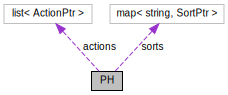
\includegraphics[width=300pt]{classPH__coll__graph}
\end{center}
\end{figure}
\subsection*{Public Member Functions}
\begin{DoxyCompactItemize}
\item 
\hypertarget{classPH_ae3ab2dd87b4bfadf04c1a14c6091aebc}{\hyperlink{classPH_ae3ab2dd87b4bfadf04c1a14c6091aebc}{P\+H} ()}\label{classPH_ae3ab2dd87b4bfadf04c1a14c6091aebc}

\begin{DoxyCompactList}\small\item\em constructor \end{DoxyCompactList}\item 
void \hyperlink{classPH_ad4335e01899c57e6802021f1afb83e7f}{add\+Sort} (Sort\+Ptr s)
\begin{DoxyCompactList}\small\item\em adds a sort to the \hyperlink{classPH}{P\+H} \end{DoxyCompactList}\item 
void \hyperlink{classPH_ae9bed9356d272f3c43f2147d6d8e5906}{add\+Action} (Action\+Ptr a)
\begin{DoxyCompactList}\small\item\em adds an action to the \hyperlink{classPH}{P\+H} \end{DoxyCompactList}\item 
\hypertarget{classPH_a02f1cd90c270555a50c08caa0fb2d491}{Sort\+Ptr \hyperlink{classPH_a02f1cd90c270555a50c08caa0fb2d491}{get\+Sort} (string const \&)}\label{classPH_a02f1cd90c270555a50c08caa0fb2d491}

\begin{DoxyCompactList}\small\item\em getter for a sort \end{DoxyCompactList}\item 
\hypertarget{classPH_ae3ae50b901b63902ae4fc3262661bb5b}{list$<$ Action\+Ptr $>$ \hyperlink{classPH_ae3ae50b901b63902ae4fc3262661bb5b}{get\+Actions} (void)}\label{classPH_ae3ae50b901b63902ae4fc3262661bb5b}

\begin{DoxyCompactList}\small\item\em getter for the actions of the \hyperlink{classPH}{P\+H} \end{DoxyCompactList}\item 
\hypertarget{classPH_a99fd490a23ae915881d9d73f0b4cbfc5}{list$<$ Sort\+Ptr $>$ \hyperlink{classPH_a99fd490a23ae915881d9d73f0b4cbfc5}{get\+Sorts} (void)}\label{classPH_a99fd490a23ae915881d9d73f0b4cbfc5}

\begin{DoxyCompactList}\small\item\em getter for the sorts of the \hyperlink{classPH}{P\+H} \end{DoxyCompactList}\item 
\hypertarget{classPH_a3c8c9ef16c7c10ad3ca83c633b2e6255}{list$<$ Process\+Ptr $>$ \hyperlink{classPH_a3c8c9ef16c7c10ad3ca83c633b2e6255}{get\+Processes} (void)}\label{classPH_a3c8c9ef16c7c10ad3ca83c633b2e6255}

\begin{DoxyCompactList}\small\item\em getter for the processes of the \hyperlink{classPH}{P\+H} \end{DoxyCompactList}\item 
string \hyperlink{classPH_ae870206aad796943dffaa6bab1f7f293}{to\+String} (void)
\begin{DoxyCompactList}\small\item\em gives a text representation of the process hitting (as it would be in a .ph file) \end{DoxyCompactList}\item 
string \hyperlink{classPH_aa0a7716cb565380f06670517609ee960}{to\+Dot\+String} (void)
\begin{DoxyCompactList}\small\item\em gives a text representation of the process hitting (in .dot format, used in Graphviz) \end{DoxyCompactList}\item 
void \hyperlink{classPH_af1f67304076aded44a15a30aed6dc652}{render} (void)
\begin{DoxyCompactList}\small\item\em calls for the process hitting in its scene \end{DoxyCompactList}\item 
G\+V\+Skeleton\+Graph\+Ptr \hyperlink{classPH_aedd3200ed6657a0a793f5ffb60dac9a5}{create\+Skeleton\+Graph} (void)
\begin{DoxyCompactList}\small\item\em make the skeleton\+Graph related to the ph model \end{DoxyCompactList}\item 
P\+H\+Scene\+Ptr \hyperlink{classPH_aaf75a785bb9bd06cec611f0fb69d05f6}{get\+Graphics\+Scene} (void)
\begin{DoxyCompactList}\small\item\em outputs for display \end{DoxyCompactList}\item 
\hypertarget{classPH_a0494ca8a53e983230a9df06fa71043e1}{int \hyperlink{classPH_a0494ca8a53e983230a9df06fa71043e1}{get\+Stochasticity\+Absorption} ()}\label{classPH_a0494ca8a53e983230a9df06fa71043e1}

\begin{DoxyCompactList}\small\item\em getter for the stochasticity absorption \end{DoxyCompactList}\item 
\hypertarget{classPH_a78fb558177760ed0e640d8a0aaf8b06a}{void \hyperlink{classPH_a78fb558177760ed0e640d8a0aaf8b06a}{set\+Stochasticity\+Absorption} (int sa)}\label{classPH_a78fb558177760ed0e640d8a0aaf8b06a}

\begin{DoxyCompactList}\small\item\em setter for the stochasticity absorption \end{DoxyCompactList}\item 
\hypertarget{classPH_aa64e3d43f773122df2329491f6abdf6c}{double \hyperlink{classPH_aa64e3d43f773122df2329491f6abdf6c}{get\+Default\+Rate} ()}\label{classPH_aa64e3d43f773122df2329491f6abdf6c}

\begin{DoxyCompactList}\small\item\em getter for the default rate; \end{DoxyCompactList}\item 
\hypertarget{classPH_ae49be2823d5a2a7c6517b6783cf9fdfa}{void \hyperlink{classPH_ae49be2823d5a2a7c6517b6783cf9fdfa}{set\+Default\+Rate} (double r)}\label{classPH_ae49be2823d5a2a7c6517b6783cf9fdfa}

\begin{DoxyCompactList}\small\item\em setter for the default rate \end{DoxyCompactList}\item 
\hypertarget{classPH_a7ede855d04ee8e3a20beb159c5520003}{bool \hyperlink{classPH_a7ede855d04ee8e3a20beb159c5520003}{get\+Infinite\+Default\+Rate} ()}\label{classPH_a7ede855d04ee8e3a20beb159c5520003}

\begin{DoxyCompactList}\small\item\em getter for the Infinite Default Rate \end{DoxyCompactList}\item 
\hypertarget{classPH_acc38a15dc0e29ddfd2c8ae7d3371f7ab}{void \hyperlink{classPH_acc38a15dc0e29ddfd2c8ae7d3371f7ab}{set\+Infinite\+Default\+Rate} (bool b)}\label{classPH_acc38a15dc0e29ddfd2c8ae7d3371f7ab}

\begin{DoxyCompactList}\small\item\em setter for the Infinitite Default Rate \end{DoxyCompactList}\end{DoxyCompactItemize}
\subsection*{Public Attributes}
\begin{DoxyCompactItemize}
\item 
\hypertarget{classPH_a4833770f4b4188111f13078d108c281e}{Q\+String\+List $\ast$ {\bfseries position\+Hit}}\label{classPH_a4833770f4b4188111f13078d108c281e}

\end{DoxyCompactItemize}
\subsection*{Protected Attributes}
\begin{DoxyCompactItemize}
\item 
\hypertarget{classPH_abdd55c7db00c19b89de0afba20d97b24}{int \hyperlink{classPH_abdd55c7db00c19b89de0afba20d97b24}{stochasticity\+\_\+absorption}}\label{classPH_abdd55c7db00c19b89de0afba20d97b24}

\begin{DoxyCompactList}\small\item\em default value for stochasticity absorption \end{DoxyCompactList}\item 
bool \hyperlink{classPH_aa66efaf095a379c3b108a023d7c98afa}{infinite\+\_\+default\+\_\+rate}
\begin{DoxyCompactList}\small\item\em boolean to know if the default rate is or is not infinite \end{DoxyCompactList}\item 
\hypertarget{classPH_a7a9525bc83257efefbaf9e78d96723ca}{double \hyperlink{classPH_a7a9525bc83257efefbaf9e78d96723ca}{default\+\_\+rate}}\label{classPH_a7a9525bc83257efefbaf9e78d96723ca}

\begin{DoxyCompactList}\small\item\em default value for rate \end{DoxyCompactList}\item 
\hypertarget{classPH_a889cc129633e88e4257f56dec04c5bac}{map$<$ string, Sort\+Ptr $>$ \hyperlink{classPH_a889cc129633e88e4257f56dec04c5bac}{sorts}}\label{classPH_a889cc129633e88e4257f56dec04c5bac}

\begin{DoxyCompactList}\small\item\em map of the sorts, linked with their names \end{DoxyCompactList}\item 
\hypertarget{classPH_a730f2eb0cd79487213cac9565d746a05}{list$<$ Action\+Ptr $>$ \hyperlink{classPH_a730f2eb0cd79487213cac9565d746a05}{actions}}\label{classPH_a730f2eb0cd79487213cac9565d746a05}

\begin{DoxyCompactList}\small\item\em list of the actions \end{DoxyCompactList}\item 
\hypertarget{classPH_ac8fbe29746ee4097c879be0cf75f3ad7}{P\+H\+Scene\+Ptr \hyperlink{classPH_ac8fbe29746ee4097c879be0cf75f3ad7}{scene}}\label{classPH_ac8fbe29746ee4097c879be0cf75f3ad7}

\begin{DoxyCompactList}\small\item\em graphical object representing the process hitting \end{DoxyCompactList}\end{DoxyCompactItemize}


\subsection{Detailed Description}
represents an entire process hitting as defined in a \hyperlink{classPH}{P\+H} file 

Definition at line 48 of file P\+H.\+h.



\subsection{Member Function Documentation}
\hypertarget{classPH_ae9bed9356d272f3c43f2147d6d8e5906}{\index{P\+H@{P\+H}!add\+Action@{add\+Action}}
\index{add\+Action@{add\+Action}!P\+H@{P\+H}}
\subsubsection[{add\+Action}]{\setlength{\rightskip}{0pt plus 5cm}void P\+H\+::add\+Action (
\begin{DoxyParamCaption}
\item[{Action\+Ptr}]{a}
\end{DoxyParamCaption}
)}}\label{classPH_ae9bed9356d272f3c43f2147d6d8e5906}


adds an action to the \hyperlink{classPH}{P\+H} 


\begin{DoxyParams}{Parameters}
{\em Action\+Ptr} & the action to add \\
\hline
\end{DoxyParams}


Definition at line 65 of file P\+H.\+cpp.


\begin{DoxyCode}
65                                \{
66     \hyperlink{classPH_a730f2eb0cd79487213cac9565d746a05}{actions}.push\_back(a);
67 \}
\end{DoxyCode}
\hypertarget{classPH_ad4335e01899c57e6802021f1afb83e7f}{\index{P\+H@{P\+H}!add\+Sort@{add\+Sort}}
\index{add\+Sort@{add\+Sort}!P\+H@{P\+H}}
\subsubsection[{add\+Sort}]{\setlength{\rightskip}{0pt plus 5cm}void P\+H\+::add\+Sort (
\begin{DoxyParamCaption}
\item[{Sort\+Ptr}]{s}
\end{DoxyParamCaption}
)}}\label{classPH_ad4335e01899c57e6802021f1afb83e7f}


adds a sort to the \hyperlink{classPH}{P\+H} 


\begin{DoxyParams}{Parameters}
{\em Sort\+Ptr} & the sort to add \\
\hline
\end{DoxyParams}


Definition at line 62 of file P\+H.\+cpp.


\begin{DoxyCode}
62                            \{
63     \hyperlink{classPH_a889cc129633e88e4257f56dec04c5bac}{sorts}.insert(SortEntry(s->getName(), s));
64 \}
\end{DoxyCode}
\hypertarget{classPH_aedd3200ed6657a0a793f5ffb60dac9a5}{\index{P\+H@{P\+H}!create\+Skeleton\+Graph@{create\+Skeleton\+Graph}}
\index{create\+Skeleton\+Graph@{create\+Skeleton\+Graph}!P\+H@{P\+H}}
\subsubsection[{create\+Skeleton\+Graph}]{\setlength{\rightskip}{0pt plus 5cm}G\+V\+Skeleton\+Graph\+Ptr P\+H\+::create\+Skeleton\+Graph (
\begin{DoxyParamCaption}
\item[{void}]{}
\end{DoxyParamCaption}
)}}\label{classPH_aedd3200ed6657a0a793f5ffb60dac9a5}


make the skeleton\+Graph related to the ph model 

calls graphviz to calculate the optimized graph \begin{DoxyReturn}{Returns}
G\+V\+Skeleton\+Graph\+Ptr pointer to the Graph built representing the skeleton 
\end{DoxyReturn}


Definition at line 104 of file P\+H.\+cpp.


\begin{DoxyCode}
104                                                \{
105     GVSkeletonGraphPtr gSkeleton = make\_shared<GVSkeletonGraph>(QString(\textcolor{stringliteral}{"Skeleton Graph"}));
106     QString sortName;
107     vector<ProcessPtr> listProcess;
108     \textcolor{keywordtype}{int} nbProcess;
109     \textcolor{keywordflow}{for}(\textcolor{keyword}{auto} &e : \hyperlink{classPH_a889cc129633e88e4257f56dec04c5bac}{sorts}) \{
110         sortName = makeSkeletonNodeName(e.second->getName());
111         listProcess = e.second->getProcesses();
112         nbProcess = listProcess.size();
113         \textcolor{keywordtype}{int} height = (nbProcess+1)*(GProcess::sizeDefault+2*GSort::marginDefault);
114         \textcolor{keywordtype}{int} width = height; \textcolor{comment}{// modified to get less "vertical" graphs}
115         gSkeleton->addNode(sortName);
116         gSkeleton->setNodeSize(gSkeleton->getNode(sortName),width,height);
117         gSkeleton->setGraphObjectAttributes(gSkeleton->getNode(sortName),\textcolor{stringliteral}{"fixedsize"},\textcolor{stringliteral}{"true"});
118     \}
119 
120     \textcolor{keywordflow}{for} (ActionPtr &a : \hyperlink{classPH_a730f2eb0cd79487213cac9565d746a05}{actions}) \{
121         QString sourceName = makeSkeletonNodeName(a->getSource()->getSort()->getName());
122         QString targetName = makeSkeletonNodeName(a->getTarget()->getSort()->getName());
123         \textcolor{keywordflow}{if}(!gSkeleton->connectionExists(sourceName,targetName)&&(QString::compare(sourceName,targetName)!=0
      )) \{
124             gSkeleton->addEdge(sourceName,targetName);
125         \}
126     \}
127     gSkeleton->applyLayout();
128 
129 
130     \textcolor{keywordflow}{return} gSkeleton;
131 \}
\end{DoxyCode}
\hypertarget{classPH_aaf75a785bb9bd06cec611f0fb69d05f6}{\index{P\+H@{P\+H}!get\+Graphics\+Scene@{get\+Graphics\+Scene}}
\index{get\+Graphics\+Scene@{get\+Graphics\+Scene}!P\+H@{P\+H}}
\subsubsection[{get\+Graphics\+Scene}]{\setlength{\rightskip}{0pt plus 5cm}P\+H\+Scene\+Ptr P\+H\+::get\+Graphics\+Scene (
\begin{DoxyParamCaption}
\item[{void}]{}
\end{DoxyParamCaption}
)}}\label{classPH_aaf75a785bb9bd06cec611f0fb69d05f6}


outputs for display 

\begin{DoxyReturn}{Returns}
P\+H\+Scene\+Ptr pointer to the Scene built 
\end{DoxyReturn}


Definition at line 33 of file P\+H.\+cpp.


\begin{DoxyCode}
33                                 \{
34     \textcolor{keywordflow}{if} (\hyperlink{classPH_ac8fbe29746ee4097c879be0cf75f3ad7}{scene}.use\_count() == 0)    \hyperlink{classPH_ac8fbe29746ee4097c879be0cf75f3ad7}{scene} = make\_shared<PHScene>(\textcolor{keyword}{this});
35     \textcolor{keywordflow}{return} \hyperlink{classPH_ac8fbe29746ee4097c879be0cf75f3ad7}{scene};
36 \}
\end{DoxyCode}
\hypertarget{classPH_af1f67304076aded44a15a30aed6dc652}{\index{P\+H@{P\+H}!render@{render}}
\index{render@{render}!P\+H@{P\+H}}
\subsubsection[{render}]{\setlength{\rightskip}{0pt plus 5cm}void P\+H\+::render (
\begin{DoxyParamCaption}
\item[{void}]{}
\end{DoxyParamCaption}
)}}\label{classPH_af1f67304076aded44a15a30aed6dc652}


calls for the process hitting in its scene 

time-\/expensive method, calls the to\+G\+V\+Graph method 

Definition at line 27 of file P\+H.\+cpp.


\begin{DoxyCode}
27                  \{
28     \textcolor{keywordflow}{if} (\hyperlink{classPH_ac8fbe29746ee4097c879be0cf75f3ad7}{scene}.use\_count() == 0) \hyperlink{classPH_ac8fbe29746ee4097c879be0cf75f3ad7}{scene} = make\_shared<PHScene>(\textcolor{keyword}{this});
29     \hyperlink{classPH_ac8fbe29746ee4097c879be0cf75f3ad7}{scene}->drawFromSkeleton();
30 \}
\end{DoxyCode}
\hypertarget{classPH_aa0a7716cb565380f06670517609ee960}{\index{P\+H@{P\+H}!to\+Dot\+String@{to\+Dot\+String}}
\index{to\+Dot\+String@{to\+Dot\+String}!P\+H@{P\+H}}
\subsubsection[{to\+Dot\+String}]{\setlength{\rightskip}{0pt plus 5cm}string P\+H\+::to\+Dot\+String (
\begin{DoxyParamCaption}
\item[{void}]{}
\end{DoxyParamCaption}
)}}\label{classPH_aa0a7716cb565380f06670517609ee960}


gives a text representation of the process hitting (in .dot format, used in Graphviz) 

\begin{DoxyReturn}{Returns}
string the text representation of the process hitting in D\+O\+T format 
\end{DoxyReturn}


Definition at line 134 of file P\+H.\+cpp.


\begin{DoxyCode}
134                             \{
135 
136     \textcolor{keywordtype}{string} res;
137     res += \textcolor{stringliteral}{"digraph G \{\(\backslash\)n"};
138     res += \textcolor{stringliteral}{"node [style=filled,color=lightgrey]\(\backslash\)n"};
139     \textcolor{comment}{// res += "edge [samehead]\(\backslash\)n";}
140 
141     \textcolor{comment}{// output Sorts}
142     res += \textcolor{stringliteral}{"\(\backslash\)n\(\backslash\)n"};
143     \textcolor{keywordflow}{for} (\textcolor{keyword}{auto} &e : \hyperlink{classPH_a889cc129633e88e4257f56dec04c5bac}{sorts})
144         res += e.second->toDotString() + \textcolor{stringliteral}{"\(\backslash\)n"};
145 
146     \textcolor{comment}{// output Actions}
147     res += \textcolor{stringliteral}{"\(\backslash\)n\(\backslash\)n"};
148     \textcolor{keywordflow}{for} (ActionPtr &a : \hyperlink{classPH_a730f2eb0cd79487213cac9565d746a05}{actions})
149         res += a->toDotString() + \textcolor{stringliteral}{"\(\backslash\)n"};
150     res += \textcolor{stringliteral}{"\}\(\backslash\)n"};
151 
152     \textcolor{keywordflow}{return} res;
153 \}
\end{DoxyCode}
\hypertarget{classPH_ae870206aad796943dffaa6bab1f7f293}{\index{P\+H@{P\+H}!to\+String@{to\+String}}
\index{to\+String@{to\+String}!P\+H@{P\+H}}
\subsubsection[{to\+String}]{\setlength{\rightskip}{0pt plus 5cm}string P\+H\+::to\+String (
\begin{DoxyParamCaption}
\item[{void}]{}
\end{DoxyParamCaption}
)}}\label{classPH_ae870206aad796943dffaa6bab1f7f293}


gives a text representation of the process hitting (as it would be in a .ph file) 

\begin{DoxyReturn}{Returns}
string the text representation of the process hitting in \hyperlink{classPH}{P\+H} format 
\end{DoxyReturn}


Definition at line 157 of file P\+H.\+cpp.


\begin{DoxyCode}
157                          \{
158 
159     \textcolor{keywordtype}{string} res;
160 
161     \textcolor{comment}{// output headers}
162     res += \textcolor{stringliteral}{"directive default\_rate "} + (\hyperlink{classPH_aa66efaf095a379c3b108a023d7c98afa}{infinite\_default\_rate} ? \textcolor{stringliteral}{"Inf"} :
163                                         (\hyperlink{classPH_a7a9525bc83257efefbaf9e78d96723ca}{default\_rate} == (int) 
      \hyperlink{classPH_a7a9525bc83257efefbaf9e78d96723ca}{default\_rate}) ?
164                                         boost::lexical\_cast<\textcolor{keywordtype}{string}>(\hyperlink{classPH_a7a9525bc83257efefbaf9e78d96723ca}{default\_rate}) + \textcolor{stringliteral}{"."}
165                                         :   boost::lexical\_cast<string>(
      \hyperlink{classPH_a7a9525bc83257efefbaf9e78d96723ca}{default\_rate})
166                                        ) + \textcolor{stringliteral}{"\(\backslash\)n"};
167     res += \textcolor{stringliteral}{"directive stochasticity\_absorption "} + boost::lexical\_cast<\textcolor{keywordtype}{string}>(
      \hyperlink{classPH_abdd55c7db00c19b89de0afba20d97b24}{stochasticity\_absorption}) + \textcolor{stringliteral}{"\(\backslash\)n"};
168 
169     \textcolor{comment}{// output Sorts}
170     \textcolor{keywordflow}{for} (\textcolor{keyword}{auto} &e : \hyperlink{classPH_a889cc129633e88e4257f56dec04c5bac}{sorts})
171         res += e.second->toString();
172     res += \textcolor{stringliteral}{"\(\backslash\)n"};
173 
174     \textcolor{comment}{// output actions}
175     \textcolor{keywordflow}{for} (ActionPtr &a : \hyperlink{classPH_a730f2eb0cd79487213cac9565d746a05}{actions})
176         res += a->toString();
177     res += \textcolor{stringliteral}{"\(\backslash\)n"};
178 
179     \textcolor{comment}{// output initial state}
180     \textcolor{keywordflow}{if} (!sorts.empty()) \{
181         res += \textcolor{stringliteral}{"initial\_state "};
182         list<string> l;
183         \textcolor{keywordflow}{for} (\textcolor{keyword}{auto} &e : sorts)
184             l.push\_back(e.second->getName() + \textcolor{stringliteral}{" "} + boost::lexical\_cast<\textcolor{keywordtype}{string}>(e.second->getActiveProcess(
      )->getNumber()));
185         res += boost::algorithm::join(l, \textcolor{stringliteral}{", "});
186     \}
187     res += \textcolor{stringliteral}{"\(\backslash\)n"};
188 
189     \textcolor{keywordflow}{return} res;
190 \}
\end{DoxyCode}


\subsection{Member Data Documentation}
\hypertarget{classPH_aa66efaf095a379c3b108a023d7c98afa}{\index{P\+H@{P\+H}!infinite\+\_\+default\+\_\+rate@{infinite\+\_\+default\+\_\+rate}}
\index{infinite\+\_\+default\+\_\+rate@{infinite\+\_\+default\+\_\+rate}!P\+H@{P\+H}}
\subsubsection[{infinite\+\_\+default\+\_\+rate}]{\setlength{\rightskip}{0pt plus 5cm}bool P\+H\+::infinite\+\_\+default\+\_\+rate\hspace{0.3cm}{\ttfamily [protected]}}}\label{classPH_aa66efaf095a379c3b108a023d7c98afa}


boolean to know if the default rate is or is not infinite 

if true then the value of default rate makes no sense 

Definition at line 181 of file P\+H.\+h.



The documentation for this class was generated from the following files\+:\begin{DoxyCompactItemize}
\item 
headers/\hyperlink{PH_8h}{P\+H.\+h}\item 
src/ph/P\+H.\+cpp\end{DoxyCompactItemize}

\hypertarget{structph__error}{\section{ph\+\_\+error Class Reference}
\label{structph__error}\index{ph\+\_\+error@{ph\+\_\+error}}
}


struct defining the exception called when there is an error in the \hyperlink{classPH}{P\+H} file extends \hyperlink{structexception__base}{exception\+\_\+base}  




{\ttfamily \#include $<$Exceptions.\+h$>$}



Inheritance diagram for ph\+\_\+error\+:\nopagebreak
\begin{figure}[H]
\begin{center}
\leavevmode
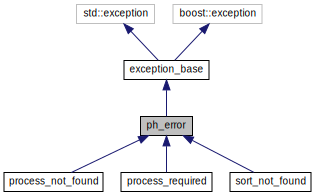
\includegraphics[width=350pt]{structph__error__inherit__graph}
\end{center}
\end{figure}


Collaboration diagram for ph\+\_\+error\+:\nopagebreak
\begin{figure}[H]
\begin{center}
\leavevmode
\includegraphics[width=266pt]{structph__error__coll__graph}
\end{center}
\end{figure}


\subsection{Detailed Description}
struct defining the exception called when there is an error in the \hyperlink{classPH}{P\+H} file extends \hyperlink{structexception__base}{exception\+\_\+base} 

Definition at line 103 of file Exceptions.\+h.



The documentation for this class was generated from the following file\+:\begin{DoxyCompactItemize}
\item 
headers/\hyperlink{Exceptions_8h}{Exceptions.\+h}\end{DoxyCompactItemize}

\hypertarget{structph__parse__error}{\section{ph\+\_\+parse\+\_\+error Class Reference}
\label{structph__parse__error}\index{ph\+\_\+parse\+\_\+error@{ph\+\_\+parse\+\_\+error}}
}


struct defining the exception called when the \hyperlink{classPH}{P\+H} file cannot be parsed extends \hyperlink{structexception__base}{exception\+\_\+base}  




{\ttfamily \#include $<$Exceptions.\+h$>$}



Inheritance diagram for ph\+\_\+parse\+\_\+error\+:\nopagebreak
\begin{figure}[H]
\begin{center}
\leavevmode
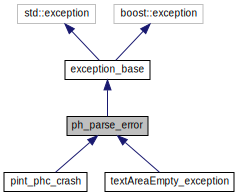
\includegraphics[width=310pt]{structph__parse__error__inherit__graph}
\end{center}
\end{figure}


Collaboration diagram for ph\+\_\+parse\+\_\+error\+:\nopagebreak
\begin{figure}[H]
\begin{center}
\leavevmode
\includegraphics[width=266pt]{structph__parse__error__coll__graph}
\end{center}
\end{figure}


\subsection{Detailed Description}
struct defining the exception called when the \hyperlink{classPH}{P\+H} file cannot be parsed extends \hyperlink{structexception__base}{exception\+\_\+base} 

Definition at line 66 of file Exceptions.\+h.



The documentation for this class was generated from the following file\+:\begin{DoxyCompactItemize}
\item 
headers/\hyperlink{Exceptions_8h}{Exceptions.\+h}\end{DoxyCompactItemize}

\hypertarget{classPHIO}{\section{P\+H\+I\+O Class Reference}
\label{classPHIO}\index{P\+H\+I\+O@{P\+H\+I\+O}}
}


manages the inputs and outputs of the \hyperlink{classPH}{P\+H} files  




{\ttfamily \#include $<$P\+H\+I\+O.\+h$>$}

\subsection*{Static Public Member Functions}
\begin{DoxyCompactItemize}
\item 
static bool \hyperlink{classPHIO_a6731852d98b581cce2a5df0984b21c07}{can\+Parse\+File} (string const \&path)
\begin{DoxyCompactList}\small\item\em checks if the file exists and is recognized by the parser \end{DoxyCompactList}\item 
static P\+H\+Ptr \hyperlink{classPHIO_a392414cadc400154232f5488fba80600}{parse\+File} (string const \&path)
\begin{DoxyCompactList}\small\item\em parses the file if it is possible \end{DoxyCompactList}\item 
static void \hyperlink{classPHIO_a383e5813d751f88a2c945d817a9204fd}{write\+To\+File} (string const \&path, P\+H\+Ptr ph)
\begin{DoxyCompactList}\small\item\em saves the \hyperlink{classPH}{P\+H} object as a \hyperlink{classPH}{P\+H} file \end{DoxyCompactList}\item 
static void \hyperlink{classPHIO_a815bbd9b063aaf8e11cd2869c950f1b4}{export\+To\+P\+N\+G} (P\+H\+Ptr ph, Q\+String name)
\begin{DoxyCompactList}\small\item\em saves as a P\+N\+G the representation of the \hyperlink{classPH}{P\+H} file as it is displayed in the G\+U\+I \end{DoxyCompactList}\item 
static void \hyperlink{classPHIO_acadc8f6f5a3595b41a05930dc810d26d}{export\+X\+M\+L\+Metadata} (\hyperlink{classMainWindow}{Main\+Window} $\ast$window, Q\+File \&output)
\begin{DoxyCompactList}\small\item\em saves as an X\+M\+L file the layout and style information of the graph displayed in G\+U\+I \end{DoxyCompactList}\item 
\hypertarget{classPHIO_a4847e266c56c53e9247c72e6dc7ac3c6}{static void {\bfseries export\+Tikz\+Metadata} (P\+H\+Ptr ph, Q\+File \&output)}\label{classPHIO_a4847e266c56c53e9247c72e6dc7ac3c6}

\end{DoxyCompactItemize}


\subsection{Detailed Description}
manages the inputs and outputs of the \hyperlink{classPH}{P\+H} files 

Definition at line 21 of file P\+H\+I\+O.\+h.



\subsection{Member Function Documentation}
\hypertarget{classPHIO_a6731852d98b581cce2a5df0984b21c07}{\index{P\+H\+I\+O@{P\+H\+I\+O}!can\+Parse\+File@{can\+Parse\+File}}
\index{can\+Parse\+File@{can\+Parse\+File}!P\+H\+I\+O@{P\+H\+I\+O}}
\subsubsection[{can\+Parse\+File}]{\setlength{\rightskip}{0pt plus 5cm}bool P\+H\+I\+O\+::can\+Parse\+File (
\begin{DoxyParamCaption}
\item[{string const \&}]{path}
\end{DoxyParamCaption}
)\hspace{0.3cm}{\ttfamily [static]}}}\label{classPHIO_a6731852d98b581cce2a5df0984b21c07}


checks if the file exists and is recognized by the parser 


\begin{DoxyParams}{Parameters}
{\em string} & the path of the file to parse \\
\hline
\end{DoxyParams}
\begin{DoxyReturn}{Returns}
bool true if the file can be parsed 
\end{DoxyReturn}


Definition at line 169 of file P\+H\+I\+O.\+cpp.


\begin{DoxyCode}
169                                            \{
170     \textcolor{keywordflow}{try} \{
171         \hyperlink{classPHIO_a392414cadc400154232f5488fba80600}{parseFile}(path);
172     \} \textcolor{keywordflow}{catch} (\hyperlink{structexception__base}{exception\_base}& x) \{
173         \textcolor{keywordflow}{return} \textcolor{keyword}{false};
174     \}
175     \textcolor{keywordflow}{return} \textcolor{keyword}{true};
176 \}
\end{DoxyCode}
\hypertarget{classPHIO_a815bbd9b063aaf8e11cd2869c950f1b4}{\index{P\+H\+I\+O@{P\+H\+I\+O}!export\+To\+P\+N\+G@{export\+To\+P\+N\+G}}
\index{export\+To\+P\+N\+G@{export\+To\+P\+N\+G}!P\+H\+I\+O@{P\+H\+I\+O}}
\subsubsection[{export\+To\+P\+N\+G}]{\setlength{\rightskip}{0pt plus 5cm}void P\+H\+I\+O\+::export\+To\+P\+N\+G (
\begin{DoxyParamCaption}
\item[{P\+H\+Ptr}]{ph, }
\item[{Q\+String}]{name}
\end{DoxyParamCaption}
)\hspace{0.3cm}{\ttfamily [static]}}}\label{classPHIO_a815bbd9b063aaf8e11cd2869c950f1b4}


saves as a P\+N\+G the representation of the \hyperlink{classPH}{P\+H} file as it is displayed in the G\+U\+I 


\begin{DoxyParams}{Parameters}
{\em P\+H\+Ptr} & pointer to the \hyperlink{classPH}{P\+H} object of the active window \\
\hline
{\em Q\+String} & the name of the file saved \\
\hline
\end{DoxyParams}


Definition at line 186 of file P\+H\+I\+O.\+cpp.


\begin{DoxyCode}
186                                              \{
187 
188     \textcolor{comment}{// create the image and render it}
189     \textcolor{comment}{// TODO make margins (currently: 4 pixels) configuration variables}
190     QImage* image = \textcolor{keyword}{new} QImage(ph->getGraphicsScene()->width()+4, ph->getGraphicsScene()->height()+4, 
      QImage::Format\_ARGB32\_Premultiplied);
191     QPainter* p = \textcolor{keyword}{new} QPainter();
192     p->begin(image);
193     p->setRenderHint(QPainter::Antialiasing);
194     ph->getGraphicsScene()->render(p);
195     p->end();
196 
197     \textcolor{comment}{// add .png to the name if necessary}
198     \textcolor{keywordflow}{if} (name.indexOf(QString(\textcolor{stringliteral}{".png"}), 0, Qt::CaseInsensitive) < 0)
199         name += \textcolor{stringliteral}{".png"};
200 
201     \textcolor{comment}{// save it}
202     image->save(name, \textcolor{stringliteral}{"PNG"});
203 \}
\end{DoxyCode}
\hypertarget{classPHIO_acadc8f6f5a3595b41a05930dc810d26d}{\index{P\+H\+I\+O@{P\+H\+I\+O}!export\+X\+M\+L\+Metadata@{export\+X\+M\+L\+Metadata}}
\index{export\+X\+M\+L\+Metadata@{export\+X\+M\+L\+Metadata}!P\+H\+I\+O@{P\+H\+I\+O}}
\subsubsection[{export\+X\+M\+L\+Metadata}]{\setlength{\rightskip}{0pt plus 5cm}void P\+H\+I\+O\+::export\+X\+M\+L\+Metadata (
\begin{DoxyParamCaption}
\item[{{\bf Main\+Window} $\ast$}]{window, }
\item[{Q\+File \&}]{output}
\end{DoxyParamCaption}
)\hspace{0.3cm}{\ttfamily [static]}}}\label{classPHIO_acadc8f6f5a3595b41a05930dc810d26d}


saves as an X\+M\+L file the layout and style information of the graph displayed in G\+U\+I 


\begin{DoxyParams}{Parameters}
{\em \hyperlink{classMainWindow}{Main\+Window}} & active \hyperlink{classMainWindow}{Main\+Window} \\
\hline
{\em Q\+File} & the file to be written \\
\hline
\end{DoxyParams}


Definition at line 207 of file P\+H\+I\+O.\+cpp.


\begin{DoxyCode}
207                                                               \{
208 
209     QXmlStreamWriter stream(&output);
210 
211     \hyperlink{classArea}{Area}* area = (\hyperlink{classArea}{Area}*)window->\hyperlink{classMainWindow_a7ef4a7c09626b415053b30bc412a3b1f}{getCentraleArea}()->currentSubWindow()->widget();
212     \hyperlink{classMyArea}{MyArea}* myarea = ((\hyperlink{classArea}{Area}*)window->\hyperlink{classMainWindow_a7ef4a7c09626b415053b30bc412a3b1f}{getCentraleArea}()->currentSubWindow()->widget
      ())->myArea;
213     QList<QTreeWidgetItem*> sortsFound = area->\hyperlink{classArea_a950b6ed9a4e754ef1a7879b727ea8749}{treeArea}->\hyperlink{classTreeArea_ab3cf8ca35655b0bace24a7c46170852f}{groupsTree}->findItems(\textcolor{stringliteral}{""}, 
      Qt::MatchContains, 0);
214     stream.setAutoFormatting(\textcolor{keyword}{true});
215     stream.writeStartDocument();
216 
217     stream.writeStartElement(\textcolor{stringliteral}{"graph\_metadata"});
218     stream.writeStartElement(\textcolor{stringliteral}{"global"});
219 
220     stream.writeStartElement(\textcolor{stringliteral}{"ph\_file"});
221     stream.writeTextElement(\textcolor{stringliteral}{"name"}, window->\hyperlink{classMainWindow_a7ef4a7c09626b415053b30bc412a3b1f}{getCentraleArea}()->currentSubWindow()->
      windowTitle());
222     stream.writeTextElement(\textcolor{stringliteral}{"path"}, area->\hyperlink{classArea_a34549bb32869fc241c911f2c8f6e6344}{path});
223     stream.writeEndElement(); \textcolor{comment}{// ph\_file}
224 
225     stream.writeStartElement(\textcolor{stringliteral}{"styles"});
226     stream.writeTextElement(\textcolor{stringliteral}{"bg\_color"}, myarea->\hyperlink{classMyArea_a7b94b516e730ddcee16d946c76bbc2b3}{getPHPtr}()->getGraphicsScene()->backgroundBrush().
      color().name());
227     stream.writeTextElement(\textcolor{stringliteral}{"sort\_color"}, \textcolor{stringliteral}{"#073642"});
228     stream.writeTextElement(\textcolor{stringliteral}{"process\_color"}, \textcolor{stringliteral}{"#EEE8D5"});
229     stream.writeTextElement(\textcolor{stringliteral}{"text\_bg\_color"}, \textcolor{stringliteral}{"#0A0A0A"});
230     stream.writeTextElement(\textcolor{stringliteral}{"sort\_font"}, \textcolor{stringliteral}{""});
231     stream.writeTextElement(\textcolor{stringliteral}{"process\_font"}, \textcolor{stringliteral}{""});
232     stream.writeTextElement(\textcolor{stringliteral}{"text\_font"}, \textcolor{stringliteral}{"TypeWriter"});
233     stream.writeEndElement(); \textcolor{comment}{// styles}
234 
235     stream.writeStartElement(\textcolor{stringliteral}{"scene"});
236     stream.writeTextElement(\textcolor{stringliteral}{"height"}, QString::number(window->height()));
237     stream.writeTextElement(\textcolor{stringliteral}{"width"}, QString::number(window->width()));
238     stream.writeEndElement(); \textcolor{comment}{//scene}
239 
240     stream.writeEndElement(); \textcolor{comment}{// global}
241 
242     stream.writeStartElement(\textcolor{stringliteral}{"sorts"});
243     \textcolor{keywordflow}{for} (SortPtr &a: myarea->\hyperlink{classMyArea_a7b94b516e730ddcee16d946c76bbc2b3}{getPHPtr}()->getSorts()) \{
244         stream.writeStartElement(\textcolor{stringliteral}{"sort"});
245         stream.writeAttribute(\textcolor{stringliteral}{"name"}, QString::fromStdString(a->getName()));
246         stream.writeAttribute(\textcolor{stringliteral}{"visible"}, QString::number(myarea->\hyperlink{classMyArea_a7b94b516e730ddcee16d946c76bbc2b3}{getPHPtr}()->getGraphicsScene()->
      getGSort(a->getName())->\hyperlink{classGSort_a58e2a6099a59b26ffe7dafd90590bd3d}{GSort::isVisible}()));
247 
248         stream.writeStartElement(\textcolor{stringliteral}{"pos"});
249         stream.writeAttribute(\textcolor{stringliteral}{"x"},QString::number(myarea->\hyperlink{classMyArea_a7b94b516e730ddcee16d946c76bbc2b3}{getPHPtr}()->getGraphicsScene()->getGSort(
      a->getName())->x()));
250         stream.writeAttribute(\textcolor{stringliteral}{"y"},QString::number(myarea->\hyperlink{classMyArea_a7b94b516e730ddcee16d946c76bbc2b3}{getPHPtr}()->getGraphicsScene()->getGSort(
      a->getName())->y()));
251         stream.writeAttribute(\textcolor{stringliteral}{"xcluster"},QString::number(myarea->\hyperlink{classMyArea_a7b94b516e730ddcee16d946c76bbc2b3}{getPHPtr}()->getGraphicsScene()->
      getGSort(a->getName())->getLeftTopCornerPoint()->x()));
252         stream.writeAttribute(\textcolor{stringliteral}{"ycluster"},QString::number(myarea->\hyperlink{classMyArea_a7b94b516e730ddcee16d946c76bbc2b3}{getPHPtr}()->getGraphicsScene()->
      getGSort(a->getName())->getLeftTopCornerPoint()->y()));
253         stream.writeEndElement(); \textcolor{comment}{// pos}
254 
255         stream.writeStartElement(\textcolor{stringliteral}{"size"});
256         stream.writeAttribute(\textcolor{stringliteral}{"w"}, QString::number(myarea->\hyperlink{classMyArea_a7b94b516e730ddcee16d946c76bbc2b3}{getPHPtr}()->getGraphicsScene()->getGSort
      (a->getName())->boundingRect().width()));
257         stream.writeAttribute(\textcolor{stringliteral}{"h"}, QString::number(myarea->\hyperlink{classMyArea_a7b94b516e730ddcee16d946c76bbc2b3}{getPHPtr}()->getGraphicsScene()->getGSort
      (a->getName())->boundingRect().height()));
258         stream.writeEndElement(); \textcolor{comment}{// size}
259 
260         stream.writeTextElement(\textcolor{stringliteral}{"color"}, myarea->\hyperlink{classMyArea_a7b94b516e730ddcee16d946c76bbc2b3}{getPHPtr}()->getGraphicsScene()->getGSort(a->
      getName())->getRect()->brush().color().name());
261 
262         stream.writeStartElement(\textcolor{stringliteral}{"label"});
263         stream.writeAttribute(\textcolor{stringliteral}{"text"}, myarea->\hyperlink{classMyArea_a7b94b516e730ddcee16d946c76bbc2b3}{getPHPtr}()->getGraphicsScene()->getGSort(a->getName()
      )->getText()->toPlainText());
264 
265         stream.writeTextElement(\textcolor{stringliteral}{"font"}, myarea->\hyperlink{classMyArea_a7b94b516e730ddcee16d946c76bbc2b3}{getPHPtr}()->getGraphicsScene()->getGSort(a->getName
      ())->getText()->font().toString());
266 
267         stream.writeStartElement(\textcolor{stringliteral}{"pos"});
268         stream.writeAttribute(\textcolor{stringliteral}{"x"}, \textcolor{stringliteral}{""});
269         stream.writeAttribute(\textcolor{stringliteral}{"y"}, \textcolor{stringliteral}{""});
270         stream.writeEndElement(); \textcolor{comment}{//pos}
271 
272         stream.writeEndElement(); \textcolor{comment}{// label}
273 
274         stream.writeStartElement(\textcolor{stringliteral}{"processes"});
275         stream.writeAttribute(\textcolor{stringliteral}{"nb"}, QString::number(a->getProcesses().size()));
276 
277         \textcolor{keywordflow}{for} (ProcessPtr &b : a->getProcesses()) \{
278             stream.writeStartElement(\textcolor{stringliteral}{"process"});
279             stream.writeAttribute(\textcolor{stringliteral}{"i"}, QString::number(b->getNumber()));
280 
281             stream.writeStartElement(\textcolor{stringliteral}{"pos"});
282             stream.writeAttribute(\textcolor{stringliteral}{"x"}, QString::number(b->getGProcess()->getCenterPoint()->x()));
283             stream.writeAttribute(\textcolor{stringliteral}{"y"}, QString::number(b->getGProcess()->getCenterPoint()->y()));
284             stream.writeEndElement(); \textcolor{comment}{// pos}
285 
286             stream.writeStartElement(\textcolor{stringliteral}{"size"});
287             stream.writeAttribute(\textcolor{stringliteral}{"w"}, \textcolor{stringliteral}{""});
288             stream.writeAttribute(\textcolor{stringliteral}{"h"}, \textcolor{stringliteral}{""});
289             stream.writeEndElement(); \textcolor{comment}{// size}
290 
291             stream.writeEndElement(); \textcolor{comment}{// process}
292         \}
293 
294         stream.writeEndElement(); \textcolor{comment}{// processes}
295 
296         stream.writeEndElement(); \textcolor{comment}{// sort}
297     \}
298 
299     stream.writeEndElement(); \textcolor{comment}{// sorts}
300 
301     stream.writeStartElement(\textcolor{stringliteral}{"sort\_groups"});
302 
303     \textcolor{keywordflow}{for} (QTreeWidgetItem* &a : sortsFound) \{
304         \textcolor{keywordflow}{if} (a->parent() == NULL) \{
305             stream.writeStartElement(\textcolor{stringliteral}{"group"});
306             stream.writeAttribute(\textcolor{stringliteral}{"name"}, a->text(0));
307             stream.writeAttribute(\textcolor{stringliteral}{"visible"}, QString::number(!a->font(0).italic()));
308             stream.writeTextElement(\textcolor{stringliteral}{"color"}, a->foreground(0).color().name());
309             \textcolor{comment}{// sorts list}
310             \textcolor{keywordflow}{if} (a->childCount()) \{
311                 stream.writeStartElement(\textcolor{stringliteral}{"sorts\_of\_group"});
312                 \textcolor{keywordflow}{for} (\textcolor{keywordtype}{int} i(0); i < a->childCount(); i++) \{
313                     stream.writeStartElement(\textcolor{stringliteral}{"sort"});
314                     stream.writeAttribute(\textcolor{stringliteral}{"name"}, a->child(i)->text(0));
315                     stream.writeEndElement(); \textcolor{comment}{// sorts}
316                 \}
317                 stream.writeEndElement();
318             \}
319             stream.writeEndElement(); \textcolor{comment}{// group}
320         \}
321     \}
322 
323     stream.writeStartElement(\textcolor{stringliteral}{"debug"});
324     stream.writeAttribute(\textcolor{stringliteral}{"debug"},\textcolor{stringliteral}{""});
325     stream.writeEndElement();
326 
327 
328     stream.writeEndElement(); \textcolor{comment}{// sort\_groups}
329 
330     stream.writeEndElement(); \textcolor{comment}{// graph\_metadata}
331 
332     stream.writeEndDocument();
333 \}
\end{DoxyCode}
\hypertarget{classPHIO_a392414cadc400154232f5488fba80600}{\index{P\+H\+I\+O@{P\+H\+I\+O}!parse\+File@{parse\+File}}
\index{parse\+File@{parse\+File}!P\+H\+I\+O@{P\+H\+I\+O}}
\subsubsection[{parse\+File}]{\setlength{\rightskip}{0pt plus 5cm}P\+H\+Ptr P\+H\+I\+O\+::parse\+File (
\begin{DoxyParamCaption}
\item[{string const \&}]{path}
\end{DoxyParamCaption}
)\hspace{0.3cm}{\ttfamily [static]}}}\label{classPHIO_a392414cadc400154232f5488fba80600}


parses the file if it is possible 


\begin{DoxyParams}{Parameters}
{\em string} & the path of the file to parse \\
\hline
\end{DoxyParams}
\begin{DoxyReturn}{Returns}
P\+H\+Ptr pointer to the \hyperlink{classPH}{P\+H} object that results form parsing 
\end{DoxyReturn}


Definition at line 136 of file P\+H\+I\+O.\+cpp.


\begin{DoxyCode}
136                                          \{
137 
138     \textcolor{comment}{// dump content using phc -l dump}
139     \textcolor{comment}{// (this command transforms complex PH instructions in basic ones)}
140     QString phc = \textcolor{stringliteral}{"phc"};
141     QStringList args;
142     args << \textcolor{stringliteral}{"-l"} << \textcolor{stringliteral}{"dump"} << \textcolor{stringliteral}{"-i"} << QString::fromUtf8(path.c\_str()) << \textcolor{stringliteral}{"--no-debug"};
143     QProcess *phcProcess = \textcolor{keyword}{new} QProcess();
144     phcProcess->start(phc, args);
145     \textcolor{keywordflow}{if} (!phcProcess->waitForStarted())
146         \textcolor{keywordflow}{throw} \hyperlink{structpint__program__not__found}{pint\_program\_not\_found}() << file\_info(\textcolor{stringliteral}{"phc"});
147 
148     \textcolor{comment}{// read result}
149     QByteArray phcStandardError;
150     QByteArray phcStandardOutput;
151     \textcolor{comment}{// Consider phc to have timed out after 10 mins}
152     \textcolor{keywordtype}{bool} timedOut = !phcProcess->waitForFinished(10*60*1000);
153     phcStandardError  += phcProcess->readAllStandardError();
154     phcStandardOutput += phcProcess->readAllStandardOutput();
155     \textcolor{keyword}{delete} phcProcess;
156 
157     \textcolor{keywordflow}{if} (timedOut)
158         \textcolor{keywordflow}{throw} \hyperlink{structpint__phc__crash}{pint\_phc\_crash}() << (parse\_info)\textcolor{stringliteral}{"Time out"};
159 
160     \textcolor{comment}{// parse dump}
161     \textcolor{keywordflow}{if} (!phcStandardError.isEmpty())
162         \textcolor{keywordflow}{throw} \hyperlink{structpint__phc__crash}{pint\_phc\_crash}() << (parse\_info)QString(phcStandardError).toStdString();
163     \textcolor{keywordflow}{return} parse(QString(phcStandardOutput).toStdString());
164 
165 \}
\end{DoxyCode}
\hypertarget{classPHIO_a383e5813d751f88a2c945d817a9204fd}{\index{P\+H\+I\+O@{P\+H\+I\+O}!write\+To\+File@{write\+To\+File}}
\index{write\+To\+File@{write\+To\+File}!P\+H\+I\+O@{P\+H\+I\+O}}
\subsubsection[{write\+To\+File}]{\setlength{\rightskip}{0pt plus 5cm}void P\+H\+I\+O\+::write\+To\+File (
\begin{DoxyParamCaption}
\item[{string const \&}]{path, }
\item[{P\+H\+Ptr}]{ph}
\end{DoxyParamCaption}
)\hspace{0.3cm}{\ttfamily [static]}}}\label{classPHIO_a383e5813d751f88a2c945d817a9204fd}


saves the \hyperlink{classPH}{P\+H} object as a \hyperlink{classPH}{P\+H} file 


\begin{DoxyParams}{Parameters}
{\em string} & the path of the file \\
\hline
{\em P\+H\+Ptr} & pointer to the object that will be saved \\
\hline
\end{DoxyParams}


Definition at line 180 of file P\+H\+I\+O.\+cpp.


\begin{DoxyCode}
180                                                     \{
181     \hyperlink{classIO_affdd7cd3e9c55cbf32551920e491cae6}{IO::writeFile}(path, ph->toString());
182 \}
\end{DoxyCode}


The documentation for this class was generated from the following files\+:\begin{DoxyCompactItemize}
\item 
headers/\hyperlink{PHIO_8h}{P\+H\+I\+O.\+h}\item 
src/io/P\+H\+I\+O.\+cpp\end{DoxyCompactItemize}

\hypertarget{classPHIOTest}{\section{P\+H\+I\+O\+Test Class Reference}
\label{classPHIOTest}\index{P\+H\+I\+O\+Test@{P\+H\+I\+O\+Test}}
}


checks that \hyperlink{classPH}{P\+H} files are parsed successfully  




{\ttfamily \#include $<$P\+H\+I\+O\+Test.\+h$>$}



Inheritance diagram for P\+H\+I\+O\+Test\+:\nopagebreak
\begin{figure}[H]
\begin{center}
\leavevmode
\includegraphics[width=141pt]{classPHIOTest__inherit__graph}
\end{center}
\end{figure}


Collaboration diagram for P\+H\+I\+O\+Test\+:\nopagebreak
\begin{figure}[H]
\begin{center}
\leavevmode
\includegraphics[width=141pt]{classPHIOTest__coll__graph}
\end{center}
\end{figure}


\subsection{Detailed Description}
checks that \hyperlink{classPH}{P\+H} files are parsed successfully 

Definition at line 13 of file P\+H\+I\+O\+Test.\+h.



The documentation for this class was generated from the following files\+:\begin{DoxyCompactItemize}
\item 
headers/test/\hyperlink{PHIOTest_8h}{P\+H\+I\+O\+Test.\+h}\item 
src/test/P\+H\+I\+O\+Test.\+cpp\end{DoxyCompactItemize}

\hypertarget{classPHScene}{\section{P\+H\+Scene Class Reference}
\label{classPHScene}\index{P\+H\+Scene@{P\+H\+Scene}}
}


the graphic object representing the process hitting extends Q\+Graphics\+Scene  




{\ttfamily \#include $<$P\+H\+Scene.\+h$>$}



Inheritance diagram for P\+H\+Scene\+:\nopagebreak
\begin{figure}[H]
\begin{center}
\leavevmode
\includegraphics[width=171pt]{classPHScene__inherit__graph}
\end{center}
\end{figure}


Collaboration diagram for P\+H\+Scene\+:\nopagebreak
\begin{figure}[H]
\begin{center}
\leavevmode
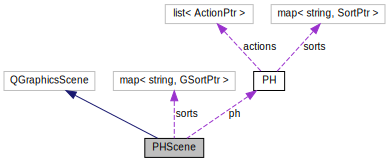
\includegraphics[width=350pt]{classPHScene__coll__graph}
\end{center}
\end{figure}
\subsection*{Public Member Functions}
\begin{DoxyCompactItemize}
\item 
\hyperlink{classPHScene_ab911261388ccc14254980b5d01909d61}{P\+H\+Scene} (\hyperlink{classPH}{P\+H} $\ast$\+\_\+ph)
\begin{DoxyCompactList}\small\item\em constructor \end{DoxyCompactList}\item 
\hypertarget{classPHScene_a8c1d06d0ad738207ecb8754537954ed5}{void \hyperlink{classPHScene_a8c1d06d0ad738207ecb8754537954ed5}{draw\+From\+Skeleton} (void)}\label{classPHScene_a8c1d06d0ad738207ecb8754537954ed5}

\begin{DoxyCompactList}\small\item\em create a \hyperlink{classGVSkeletonGraph}{G\+V\+Skeleton\+Graph} from the \hyperlink{classPH}{P\+H} object, then draw the P\+H\+S\+Cene from it \end{DoxyCompactList}\item 
G\+Sort\+Ptr \hyperlink{classPHScene_ae8be020b063c06f135d644937d65147b}{get\+G\+Sort} (const string \&s)
\begin{DoxyCompactList}\small\item\em gets a \hyperlink{classGSort}{G\+Sort} by its related \hyperlink{classSort}{Sort}'s name \end{DoxyCompactList}\item 
\hypertarget{classPHScene_a4c7995ab5b0807000aa1234edbb44794}{map$<$ string, G\+Sort\+Ptr $>$ \hyperlink{classPHScene_a4c7995ab5b0807000aa1234edbb44794}{get\+G\+Sorts} ()}\label{classPHScene_a4c7995ab5b0807000aa1234edbb44794}

\begin{DoxyCompactList}\small\item\em getter for sorts \end{DoxyCompactList}\item 
\hypertarget{classPHScene_a89518baed691958147d7f55a25d14f9c}{std\+::vector$<$ G\+Process\+Ptr $>$ \hyperlink{classPHScene_a89518baed691958147d7f55a25d14f9c}{get\+Processes} ()}\label{classPHScene_a89518baed691958147d7f55a25d14f9c}

\begin{DoxyCompactList}\small\item\em get the processes \end{DoxyCompactList}\item 
\hypertarget{classPHScene_a4cf1a2937e804ad79a0c490f7be6ef45}{std\+::vector$<$ G\+Action\+Ptr $>$ \hyperlink{classPHScene_a4cf1a2937e804ad79a0c490f7be6ef45}{get\+Actions} ()}\label{classPHScene_a4cf1a2937e804ad79a0c490f7be6ef45}

\begin{DoxyCompactList}\small\item\em get the actions \end{DoxyCompactList}\item 
\hypertarget{classPHScene_a176668ca3774e8fec7ac7902e70c048e}{void \hyperlink{classPHScene_a176668ca3774e8fec7ac7902e70c048e}{update\+Actions} ()}\label{classPHScene_a176668ca3774e8fec7ac7902e70c048e}

\begin{DoxyCompactList}\small\item\em update the position of actions \end{DoxyCompactList}\item 
void \hyperlink{classPHScene_a4a99c9817b8ecbecf161e928d4e90984}{set\+Simple\+Display} (bool on\+Off)
\begin{DoxyCompactList}\small\item\em switch the display mode between detailled/simplified \end{DoxyCompactList}\item 
void \hyperlink{classPHScene_a9b080cb754ca9b12c2811d186e6f34b6}{context\+Menu\+Event} (Q\+Graphics\+Scene\+Context\+Menu\+Event $\ast$event)
\begin{DoxyCompactList}\small\item\em Handles mouse press event (handles drag start) \end{DoxyCompactList}\item 
\hypertarget{classPHScene_a865f5d4e8e1a62ea4cccc9a08761f3b7}{void \hyperlink{classPHScene_a865f5d4e8e1a62ea4cccc9a08761f3b7}{Background\+Color} ()}\label{classPHScene_a865f5d4e8e1a62ea4cccc9a08761f3b7}

\begin{DoxyCompactList}\small\item\em change the color of the background \end{DoxyCompactList}\item 
\hypertarget{classPHScene_ae49485e4ddf79c5d71aba4a4aebf147d}{void \hyperlink{classPHScene_ae49485e4ddf79c5d71aba4a4aebf147d}{Actions\+In\+Bold} ()}\label{classPHScene_ae49485e4ddf79c5d71aba4a4aebf147d}

\begin{DoxyCompactList}\small\item\em change the actions in bold \end{DoxyCompactList}\item 
\hypertarget{classPHScene_a648b16c898a66ac5e4a574e865617671}{void \hyperlink{classPHScene_a648b16c898a66ac5e4a574e865617671}{Action\+Color} ()}\label{classPHScene_a648b16c898a66ac5e4a574e865617671}

\begin{DoxyCompactList}\small\item\em change the color of the action \end{DoxyCompactList}\end{DoxyCompactItemize}
\subsection*{Protected Member Functions}
\begin{DoxyCompactItemize}
\item 
\hypertarget{classPHScene_a63a2e3d0f466494e545d2d8d9dea1e86}{void \hyperlink{classPHScene_a63a2e3d0f466494e545d2d8d9dea1e86}{create\+Actions} ()}\label{classPHScene_a63a2e3d0f466494e545d2d8d9dea1e86}

\begin{DoxyCompactList}\small\item\em creates \hyperlink{classGAction}{G\+Action} items from graphviz graph (\hyperlink{structGVEdge}{G\+V\+Edge} structs) \end{DoxyCompactList}\end{DoxyCompactItemize}
\subsection*{Protected Attributes}
\begin{DoxyCompactItemize}
\item 
\hypertarget{classPHScene_a332655cec4c6cca3153ffc3ee14eb465}{\hyperlink{classPH}{P\+H} $\ast$ \hyperlink{classPHScene_a332655cec4c6cca3153ffc3ee14eb465}{ph}}\label{classPHScene_a332655cec4c6cca3153ffc3ee14eb465}

\begin{DoxyCompactList}\small\item\em the related process hitting \end{DoxyCompactList}\item 
\hypertarget{classPHScene_a664d48bb0ae4f95df04e7a939855cae5}{map$<$ string, G\+Sort\+Ptr $>$ \hyperlink{classPHScene_a664d48bb0ae4f95df04e7a939855cae5}{sorts}}\label{classPHScene_a664d48bb0ae4f95df04e7a939855cae5}

\begin{DoxyCompactList}\small\item\em map of the Sorts drawn in the scene\+: the keys are the names of the Sorts \end{DoxyCompactList}\item 
\hypertarget{classPHScene_a392d190fc16531af5049727766582bed}{std\+::vector$<$ G\+Process\+Ptr $>$ \hyperlink{classPHScene_a392d190fc16531af5049727766582bed}{processes}}\label{classPHScene_a392d190fc16531af5049727766582bed}

\begin{DoxyCompactList}\small\item\em vector of the Processes drawn in the scene \end{DoxyCompactList}\item 
\hypertarget{classPHScene_a5802a1a674ffd883d3bf8403399365fb}{std\+::vector$<$ G\+Action\+Ptr $>$ \hyperlink{classPHScene_a5802a1a674ffd883d3bf8403399365fb}{actions}}\label{classPHScene_a5802a1a674ffd883d3bf8403399365fb}

\begin{DoxyCompactList}\small\item\em vector of the Actions drawn in the scene \end{DoxyCompactList}\end{DoxyCompactItemize}


\subsection{Detailed Description}
the graphic object representing the process hitting extends Q\+Graphics\+Scene 

Definition at line 42 of file P\+H\+Scene.\+h.



\subsection{Constructor \& Destructor Documentation}
\hypertarget{classPHScene_ab911261388ccc14254980b5d01909d61}{\index{P\+H\+Scene@{P\+H\+Scene}!P\+H\+Scene@{P\+H\+Scene}}
\index{P\+H\+Scene@{P\+H\+Scene}!P\+H\+Scene@{P\+H\+Scene}}
\subsubsection[{P\+H\+Scene}]{\setlength{\rightskip}{0pt plus 5cm}P\+H\+Scene\+::\+P\+H\+Scene (
\begin{DoxyParamCaption}
\item[{{\bf P\+H} $\ast$}]{\+\_\+ph}
\end{DoxyParamCaption}
)}}\label{classPHScene_ab911261388ccc14254980b5d01909d61}


constructor 


\begin{DoxyParams}{Parameters}
{\em P\+H$\ast$} & the \hyperlink{classPH}{P\+H} graph to use \\
\hline
\end{DoxyParams}


Definition at line 17 of file P\+H\+Scene.\+cpp.


\begin{DoxyCode}
17                         : \hyperlink{classPHScene_a332655cec4c6cca3153ffc3ee14eb465}{ph}(\_ph) \{
18     \textcolor{comment}{// set background color}
19     setBackgroundBrush(QBrush(QColor(255, 255, 255)));
20 \}
\end{DoxyCode}


\subsection{Member Function Documentation}
\hypertarget{classPHScene_a9b080cb754ca9b12c2811d186e6f34b6}{\index{P\+H\+Scene@{P\+H\+Scene}!context\+Menu\+Event@{context\+Menu\+Event}}
\index{context\+Menu\+Event@{context\+Menu\+Event}!P\+H\+Scene@{P\+H\+Scene}}
\subsubsection[{context\+Menu\+Event}]{\setlength{\rightskip}{0pt plus 5cm}void P\+H\+Scene\+::context\+Menu\+Event (
\begin{DoxyParamCaption}
\item[{Q\+Graphics\+Scene\+Context\+Menu\+Event $\ast$}]{event}
\end{DoxyParamCaption}
)}}\label{classPHScene_a9b080cb754ca9b12c2811d186e6f34b6}


Handles mouse press event (handles drag start) 


\begin{DoxyParams}{Parameters}
{\em Q\+Graphics\+Scene\+Mouse\+Event} & the event to be handled \\
\hline
\end{DoxyParams}


Definition at line 93 of file P\+H\+Scene.\+cpp.


\begin{DoxyCode}
93                                                                     \{
94 
95     QPointF sorEventPressPoint;
96     \textcolor{keywordtype}{bool} horsSorte=\textcolor{keyword}{true};
97 
98     \textcolor{comment}{// if other mouse buttons are pressed, do nothing}
99     \textcolor{keywordflow}{if} (QApplication::mouseButtons() == Qt::RightButton) \{
100         \textcolor{keywordflow}{for}(\textcolor{keyword}{auto} &s : \hyperlink{classPHScene_a664d48bb0ae4f95df04e7a939855cae5}{sorts}) \{
101             sorEventPressPoint = s.second.get()->geteventPressPoint();
102             \textcolor{keywordflow}{if}(sorEventPressPoint.x() == \textcolor{keyword}{event}->scenePos().x() && sorEventPressPoint.y() == \textcolor{keyword}{event}->scenePos
      ().y()) \{
103                 horsSorte=\textcolor{keyword}{false};
104             \}
105         \}
106         \textcolor{keywordflow}{if}(horsSorte) \{
107 
108             QMenu menu;
109             QAction* switchToSimplifiedModel = menu.addAction(\textcolor{stringliteral}{"switch to simplified model"});
110             QAction* switchToDetailledModel = menu.addAction(\textcolor{stringliteral}{"switch to detailled model"});
111             QAction* switchBackgroundColor = menu.addAction(\textcolor{stringliteral}{"color background "});
112             QAction* switchActionsInBold = menu.addAction(\textcolor{stringliteral}{"all actions in bold/ not to blod"});
113             QAction* switchActionColor = menu.addAction(\textcolor{stringliteral}{"color all actions"});
114 
115             QAction* selectedAction = menu.exec(QCursor::pos());
116             \textcolor{keywordflow}{if}(selectedAction != 0) \{
117                 \textcolor{keywordflow}{if}(QString::compare(selectedAction->text(),switchBackgroundColor->text())==0) \{
118                     \hyperlink{classPHScene_a865f5d4e8e1a62ea4cccc9a08761f3b7}{BackgroundColor}();
119                 \} \textcolor{keywordflow}{else} \textcolor{keywordflow}{if}(QString::compare(selectedAction->text(),switchActionsInBold->text())==0) \{
120                     \hyperlink{classPHScene_ae49485e4ddf79c5d71aba4a4aebf147d}{ActionsInBold}();
121                 \} \textcolor{keywordflow}{else} \textcolor{keywordflow}{if}(QString::compare(selectedAction->text(),switchActionColor->text())==0) \{
122                     \hyperlink{classPHScene_a648b16c898a66ac5e4a574e865617671}{ActionColor}();
123                 \} \textcolor{keywordflow}{else} \textcolor{keywordflow}{if}(QString::compare(selectedAction->text(),switchToSimplifiedModel->text())==0) \{
124                     \hyperlink{classPHScene_a4a99c9817b8ecbecf161e928d4e90984}{setSimpleDisplay}(\textcolor{keyword}{true});
125                 \} \textcolor{keywordflow}{else} \textcolor{keywordflow}{if}(QString::compare(selectedAction->text(),switchToDetailledModel->text())==0) \{
126                     \hyperlink{classPHScene_a4a99c9817b8ecbecf161e928d4e90984}{setSimpleDisplay}(\textcolor{keyword}{false});
127                 \}
128 
129             \}
130         \}
131     \}
132 \}
\end{DoxyCode}
\hypertarget{classPHScene_ae8be020b063c06f135d644937d65147b}{\index{P\+H\+Scene@{P\+H\+Scene}!get\+G\+Sort@{get\+G\+Sort}}
\index{get\+G\+Sort@{get\+G\+Sort}!P\+H\+Scene@{P\+H\+Scene}}
\subsubsection[{get\+G\+Sort}]{\setlength{\rightskip}{0pt plus 5cm}G\+Sort\+Ptr P\+H\+Scene\+::get\+G\+Sort (
\begin{DoxyParamCaption}
\item[{const string \&}]{s}
\end{DoxyParamCaption}
)}}\label{classPHScene_ae8be020b063c06f135d644937d65147b}


gets a \hyperlink{classGSort}{G\+Sort} by its related \hyperlink{classSort}{Sort}'s name 


\begin{DoxyParams}{Parameters}
{\em string} & the name of the (G)\hyperlink{classSort}{Sort} to get \\
\hline
\end{DoxyParams}
\begin{DoxyReturn}{Returns}
G\+Sort\+Ptr pointer to the \hyperlink{classGSort}{G\+Sort} to get 
\end{DoxyReturn}


Definition at line 52 of file P\+H\+Scene.\+cpp.


\begin{DoxyCode}
52                                            \{
53     map<string, GSortPtr>::iterator f = \hyperlink{classPHScene_a664d48bb0ae4f95df04e7a939855cae5}{sorts}.find(s);
54     \textcolor{keywordflow}{if} (f == \hyperlink{classPHScene_a664d48bb0ae4f95df04e7a939855cae5}{sorts}.end())
55         \textcolor{keywordflow}{throw} \hyperlink{structsort__not__found}{sort\_not\_found}() << sort\_info(s);
56     \textcolor{keywordflow}{return} \hyperlink{classPHScene_a664d48bb0ae4f95df04e7a939855cae5}{sorts}[s];
57 \}
\end{DoxyCode}
\hypertarget{classPHScene_a4a99c9817b8ecbecf161e928d4e90984}{\index{P\+H\+Scene@{P\+H\+Scene}!set\+Simple\+Display@{set\+Simple\+Display}}
\index{set\+Simple\+Display@{set\+Simple\+Display}!P\+H\+Scene@{P\+H\+Scene}}
\subsubsection[{set\+Simple\+Display}]{\setlength{\rightskip}{0pt plus 5cm}void P\+H\+Scene\+::set\+Simple\+Display (
\begin{DoxyParamCaption}
\item[{bool}]{on\+Off}
\end{DoxyParamCaption}
)}}\label{classPHScene_a4a99c9817b8ecbecf161e928d4e90984}


switch the display mode between detailled/simplified 


\begin{DoxyParams}{Parameters}
{\em bool} & activate or not the simplified model \\
\hline
\end{DoxyParams}


Definition at line 85 of file P\+H\+Scene.\+cpp.


\begin{DoxyCode}
85                                          \{
86     \textcolor{keywordflow}{for}(\textcolor{keyword}{auto} &s : \hyperlink{classPHScene_a664d48bb0ae4f95df04e7a939855cae5}{sorts}) \{
87         s.second->setSimpleDisplay(onOff);
88     \}
89     \hyperlink{classPHScene_a176668ca3774e8fec7ac7902e70c048e}{updateActions}();
90 \}
\end{DoxyCode}


The documentation for this class was generated from the following files\+:\begin{DoxyCompactItemize}
\item 
headers/\hyperlink{PHScene_8h}{P\+H\+Scene.\+h}\item 
src/gfx/P\+H\+Scene.\+cpp\end{DoxyCompactItemize}

\hypertarget{structpint__phc__crash}{\section{pint\+\_\+phc\+\_\+crash Class Reference}
\label{structpint__phc__crash}\index{pint\+\_\+phc\+\_\+crash@{pint\+\_\+phc\+\_\+crash}}
}


struct defining the exception called when Pint cannot be called extends \hyperlink{structph__parse__error}{ph\+\_\+parse\+\_\+error}  




{\ttfamily \#include $<$Exceptions.\+h$>$}



Inheritance diagram for pint\+\_\+phc\+\_\+crash\+:\nopagebreak
\begin{figure}[H]
\begin{center}
\leavevmode
\includegraphics[width=266pt]{structpint__phc__crash__inherit__graph}
\end{center}
\end{figure}


Collaboration diagram for pint\+\_\+phc\+\_\+crash\+:\nopagebreak
\begin{figure}[H]
\begin{center}
\leavevmode
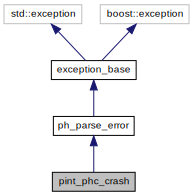
\includegraphics[width=266pt]{structpint__phc__crash__coll__graph}
\end{center}
\end{figure}


\subsection{Detailed Description}
struct defining the exception called when Pint cannot be called extends \hyperlink{structph__parse__error}{ph\+\_\+parse\+\_\+error} 

Definition at line 74 of file Exceptions.\+h.



The documentation for this class was generated from the following file\+:\begin{DoxyCompactItemize}
\item 
headers/\hyperlink{Exceptions_8h}{Exceptions.\+h}\end{DoxyCompactItemize}

\hypertarget{structpint__program__not__found}{\section{pint\+\_\+program\+\_\+not\+\_\+found Class Reference}
\label{structpint__program__not__found}\index{pint\+\_\+program\+\_\+not\+\_\+found@{pint\+\_\+program\+\_\+not\+\_\+found}}
}


struct defining the exception called when Pint is not found\$ extends \hyperlink{structexception__base}{exception\+\_\+base}  




{\ttfamily \#include $<$Exceptions.\+h$>$}



Inheritance diagram for pint\+\_\+program\+\_\+not\+\_\+found\+:\nopagebreak
\begin{figure}[H]
\begin{center}
\leavevmode
\includegraphics[width=266pt]{structpint__program__not__found__inherit__graph}
\end{center}
\end{figure}


Collaboration diagram for pint\+\_\+program\+\_\+not\+\_\+found\+:\nopagebreak
\begin{figure}[H]
\begin{center}
\leavevmode
\includegraphics[width=266pt]{structpint__program__not__found__coll__graph}
\end{center}
\end{figure}


\subsection{Detailed Description}
struct defining the exception called when Pint is not found\$ extends \hyperlink{structexception__base}{exception\+\_\+base} 

Definition at line 91 of file Exceptions.\+h.



The documentation for this class was generated from the following file\+:\begin{DoxyCompactItemize}
\item 
headers/\hyperlink{Exceptions_8h}{Exceptions.\+h}\end{DoxyCompactItemize}

\hypertarget{classProcess}{\section{Process Class Reference}
\label{classProcess}\index{Process@{Process}}
}


represents a \hyperlink{classProcess}{Process} of the process hitting  




{\ttfamily \#include $<$Process.\+h$>$}

\subsection*{Public Member Functions}
\begin{DoxyCompactItemize}
\item 
\hyperlink{classProcess_a267617e8f2cfd994e0527635372be90c}{Process} (Sort\+Ptr s, const int \&n)
\begin{DoxyCompactList}\small\item\em constructor \end{DoxyCompactList}\item 
\hypertarget{classProcess_acdfa357f41df6f1e09cdffbc5c5b2c3b}{int \hyperlink{classProcess_acdfa357f41df6f1e09cdffbc5c5b2c3b}{get\+Number} (void)}\label{classProcess_acdfa357f41df6f1e09cdffbc5c5b2c3b}

\begin{DoxyCompactList}\small\item\em gets the number \end{DoxyCompactList}\item 
\hypertarget{classProcess_aaabe803350e1d6dcc23d8aa4ff2314db}{Sort\+Ptr \hyperlink{classProcess_aaabe803350e1d6dcc23d8aa4ff2314db}{get\+Sort} (void)}\label{classProcess_aaabe803350e1d6dcc23d8aa4ff2314db}

\begin{DoxyCompactList}\small\item\em gets the \hyperlink{classSort}{Sort} \end{DoxyCompactList}\item 
string \hyperlink{classProcess_af9a89e83db6a14451104b49eac7dd313}{get\+Dot\+Name} (void)
\begin{DoxyCompactList}\small\item\em builds name for D\+O\+T files \end{DoxyCompactList}\item 
string \hyperlink{classProcess_ad9c1f2be57856c4e62d00f8494d2281f}{to\+Dot\+String} (void)
\begin{DoxyCompactList}\small\item\em gives a text representation of the process hitting (in .dot format, used in Graphviz) \end{DoxyCompactList}\item 
void \hyperlink{classProcess_a14e32beee307cf814fbc569a96951bba}{set\+G\+Process} (G\+Process\+Ptr g\+P\+Ptr)
\begin{DoxyCompactList}\small\item\em sets the related \hyperlink{classGProcess}{G\+Process} \end{DoxyCompactList}\item 
G\+Process\+Ptr \hyperlink{classProcess_af7c8dfd3af2a014c0371840ce82ed608}{get\+G\+Process} ()
\begin{DoxyCompactList}\small\item\em gets the related \hyperlink{classGProcess}{G\+Process} \end{DoxyCompactList}\end{DoxyCompactItemize}


\subsection{Detailed Description}
represents a \hyperlink{classProcess}{Process} of the process hitting 

Definition at line 32 of file Process.\+h.



\subsection{Constructor \& Destructor Documentation}
\hypertarget{classProcess_a267617e8f2cfd994e0527635372be90c}{\index{Process@{Process}!Process@{Process}}
\index{Process@{Process}!Process@{Process}}
\subsubsection[{Process}]{\setlength{\rightskip}{0pt plus 5cm}Process\+::\+Process (
\begin{DoxyParamCaption}
\item[{Sort\+Ptr}]{s, }
\item[{const int \&}]{n}
\end{DoxyParamCaption}
)}}\label{classProcess_a267617e8f2cfd994e0527635372be90c}


constructor 


\begin{DoxyParams}{Parameters}
{\em Sortptr} & pointer to the \hyperlink{classSort}{Sort} the \hyperlink{classProcess}{Process} is related to \\
\hline
{\em int} & number of the \hyperlink{classProcess}{Process} in the \hyperlink{classSort}{Sort} it is related to \\
\hline
\end{DoxyParams}


Definition at line 5 of file Process.\+cpp.


\begin{DoxyCode}
5 : sort(s), number(n) \{\}
\end{DoxyCode}


\subsection{Member Function Documentation}
\hypertarget{classProcess_af9a89e83db6a14451104b49eac7dd313}{\index{Process@{Process}!get\+Dot\+Name@{get\+Dot\+Name}}
\index{get\+Dot\+Name@{get\+Dot\+Name}!Process@{Process}}
\subsubsection[{get\+Dot\+Name}]{\setlength{\rightskip}{0pt plus 5cm}string Process\+::get\+Dot\+Name (
\begin{DoxyParamCaption}
\item[{void}]{}
\end{DoxyParamCaption}
)}}\label{classProcess_af9a89e83db6a14451104b49eac7dd313}


builds name for D\+O\+T files 

\begin{DoxyReturn}{Returns}
string adapted name 
\end{DoxyReturn}


Definition at line 16 of file Process.\+cpp.


\begin{DoxyCode}
16                             \{
17     \textcolor{keywordtype}{string} n = boost::lexical\_cast<\textcolor{keywordtype}{string}>(number);
18     \textcolor{keywordflow}{return} sort->getName() + \textcolor{stringliteral}{"\_p"} + n;
19 \}
\end{DoxyCode}
\hypertarget{classProcess_af7c8dfd3af2a014c0371840ce82ed608}{\index{Process@{Process}!get\+G\+Process@{get\+G\+Process}}
\index{get\+G\+Process@{get\+G\+Process}!Process@{Process}}
\subsubsection[{get\+G\+Process}]{\setlength{\rightskip}{0pt plus 5cm}G\+Process\+Ptr Process\+::get\+G\+Process (
\begin{DoxyParamCaption}
{}
\end{DoxyParamCaption}
)}}\label{classProcess_af7c8dfd3af2a014c0371840ce82ed608}


gets the related \hyperlink{classGProcess}{G\+Process} 

\begin{DoxyReturn}{Returns}
G\+Process\+Ptr a pointer to the related \hyperlink{classGProcess}{G\+Process} object 
\end{DoxyReturn}


Definition at line 35 of file Process.\+cpp.


\begin{DoxyCode}
35                                  \{
36     \textcolor{keywordflow}{return} gProcess;
37 \}
\end{DoxyCode}
\hypertarget{classProcess_a14e32beee307cf814fbc569a96951bba}{\index{Process@{Process}!set\+G\+Process@{set\+G\+Process}}
\index{set\+G\+Process@{set\+G\+Process}!Process@{Process}}
\subsubsection[{set\+G\+Process}]{\setlength{\rightskip}{0pt plus 5cm}void Process\+::set\+G\+Process (
\begin{DoxyParamCaption}
\item[{G\+Process\+Ptr}]{g\+P\+Ptr}
\end{DoxyParamCaption}
)}}\label{classProcess_a14e32beee307cf814fbc569a96951bba}


sets the related \hyperlink{classGProcess}{G\+Process} 


\begin{DoxyParams}{Parameters}
{\em a} & pointer to the related \hyperlink{classGProcess}{G\+Process} object \\
\hline
\end{DoxyParams}


Definition at line 23 of file Process.\+cpp.


\begin{DoxyCode}
23                                            \{
24     gProcess = gPPtr;
25 \}
\end{DoxyCode}
\hypertarget{classProcess_ad9c1f2be57856c4e62d00f8494d2281f}{\index{Process@{Process}!to\+Dot\+String@{to\+Dot\+String}}
\index{to\+Dot\+String@{to\+Dot\+String}!Process@{Process}}
\subsubsection[{to\+Dot\+String}]{\setlength{\rightskip}{0pt plus 5cm}string Process\+::to\+Dot\+String (
\begin{DoxyParamCaption}
\item[{void}]{}
\end{DoxyParamCaption}
)}}\label{classProcess_ad9c1f2be57856c4e62d00f8494d2281f}


gives a text representation of the process hitting (in .dot format, used in Graphviz) 

\begin{DoxyReturn}{Returns}
string the representation in D\+O\+T format 
\end{DoxyReturn}


Definition at line 9 of file Process.\+cpp.


\begin{DoxyCode}
9                              \{
10     \textcolor{keywordtype}{string} n = boost::lexical\_cast<\textcolor{keywordtype}{string}>(number);
11     \textcolor{keywordflow}{return} \hyperlink{classProcess_af9a89e83db6a14451104b49eac7dd313}{getDotName}() + \textcolor{stringliteral}{" [label=\(\backslash\)""} + n + \textcolor{stringliteral}{"\(\backslash\)"];\(\backslash\)n"};
12 \}
\end{DoxyCode}


The documentation for this class was generated from the following files\+:\begin{DoxyCompactItemize}
\item 
headers/\hyperlink{Process_8h}{Process.\+h}\item 
src/ph/Process.\+cpp\end{DoxyCompactItemize}

\hypertarget{structprocess__not__found}{\section{process\+\_\+not\+\_\+found Class Reference}
\label{structprocess__not__found}\index{process\+\_\+not\+\_\+found@{process\+\_\+not\+\_\+found}}
}


struct defining the exception called when the process called is not found extends \hyperlink{structph__error}{ph\+\_\+error}  




{\ttfamily \#include $<$Exceptions.\+h$>$}



Inheritance diagram for process\+\_\+not\+\_\+found\+:\nopagebreak
\begin{figure}[H]
\begin{center}
\leavevmode
\includegraphics[width=266pt]{structprocess__not__found__inherit__graph}
\end{center}
\end{figure}


Collaboration diagram for process\+\_\+not\+\_\+found\+:\nopagebreak
\begin{figure}[H]
\begin{center}
\leavevmode
\includegraphics[width=266pt]{structprocess__not__found__coll__graph}
\end{center}
\end{figure}


\subsection{Detailed Description}
struct defining the exception called when the process called is not found extends \hyperlink{structph__error}{ph\+\_\+error} 

Definition at line 119 of file Exceptions.\+h.



The documentation for this class was generated from the following file\+:\begin{DoxyCompactItemize}
\item 
headers/\hyperlink{Exceptions_8h}{Exceptions.\+h}\end{DoxyCompactItemize}

\hypertarget{structprocess__required}{\section{process\+\_\+required Class Reference}
\label{structprocess__required}\index{process\+\_\+required@{process\+\_\+required}}
}


struct defining the exception called when the process is not specified extends \hyperlink{structph__error}{ph\+\_\+error}  




{\ttfamily \#include $<$Exceptions.\+h$>$}



Inheritance diagram for process\+\_\+required\+:\nopagebreak
\begin{figure}[H]
\begin{center}
\leavevmode
\includegraphics[width=266pt]{structprocess__required__inherit__graph}
\end{center}
\end{figure}


Collaboration diagram for process\+\_\+required\+:\nopagebreak
\begin{figure}[H]
\begin{center}
\leavevmode
\includegraphics[width=266pt]{structprocess__required__coll__graph}
\end{center}
\end{figure}


\subsection{Detailed Description}
struct defining the exception called when the process is not specified extends \hyperlink{structph__error}{ph\+\_\+error} 

Definition at line 111 of file Exceptions.\+h.



The documentation for this class was generated from the following file\+:\begin{DoxyCompactItemize}
\item 
headers/\hyperlink{Exceptions_8h}{Exceptions.\+h}\end{DoxyCompactItemize}

\hypertarget{classSort}{\section{Sort Class Reference}
\label{classSort}\index{Sort@{Sort}}
}


represents a sort of the process hitting  




{\ttfamily \#include $<$Sort.\+h$>$}



Collaboration diagram for Sort\+:\nopagebreak
\begin{figure}[H]
\begin{center}
\leavevmode
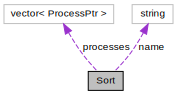
\includegraphics[width=250pt]{classSort__coll__graph}
\end{center}
\end{figure}
\subsection*{Public Member Functions}
\begin{DoxyCompactItemize}
\item 
Process\+Ptr \hyperlink{classSort_a5b30c6e6f75987a8a10bef36762aace6}{get\+Process} (const uint \&)
\begin{DoxyCompactList}\small\item\em gets a \hyperlink{classProcess}{Process} by its index \end{DoxyCompactList}\item 
\hypertarget{classSort_af4b1feed1cf830292a474110ea478b7d}{vector$<$ Process\+Ptr $>$ \hyperlink{classSort_af4b1feed1cf830292a474110ea478b7d}{get\+Processes} (void)}\label{classSort_af4b1feed1cf830292a474110ea478b7d}

\begin{DoxyCompactList}\small\item\em gets processes vector \end{DoxyCompactList}\item 
\hypertarget{classSort_ad77072a25565d843de3ea6a7b47ffbdd}{Process\+Ptr \hyperlink{classSort_ad77072a25565d843de3ea6a7b47ffbdd}{get\+Active\+Process} (void)}\label{classSort_ad77072a25565d843de3ea6a7b47ffbdd}

\begin{DoxyCompactList}\small\item\em gets the active process \end{DoxyCompactList}\item 
\hypertarget{classSort_afb60d6f4e0b2d2984faf33fe16ad29b2}{void \hyperlink{classSort_afb60d6f4e0b2d2984faf33fe16ad29b2}{set\+Active\+Process} (const int \&)}\label{classSort_afb60d6f4e0b2d2984faf33fe16ad29b2}

\begin{DoxyCompactList}\small\item\em sets the active process \end{DoxyCompactList}\item 
int \hyperlink{classSort_a1f91b39f9d5d05ffbf59a1480102e85c}{count\+Processes} (void)
\begin{DoxyCompactList}\small\item\em counts the number of processes \end{DoxyCompactList}\item 
\hypertarget{classSort_aae171b005c3dada51b7a302230ff501a}{string \hyperlink{classSort_aae171b005c3dada51b7a302230ff501a}{get\+Name} (void)}\label{classSort_aae171b005c3dada51b7a302230ff501a}

\begin{DoxyCompactList}\small\item\em gets the name of the \hyperlink{classSort}{Sort} \end{DoxyCompactList}\item 
string \hyperlink{classSort_ae160613fb2d5c7fd9818a5c7d4be992a}{to\+String} (void)
\begin{DoxyCompactList}\small\item\em gives a text representation of the process hitting (as it would be in a .ph file) \end{DoxyCompactList}\item 
string \hyperlink{classSort_a9bb67cd444d217dd477c896a31d869a0}{to\+Dot\+String} (void)
\begin{DoxyCompactList}\small\item\em gives a text representation of the process hitting (in .dot format, used in Graphviz) \end{DoxyCompactList}\end{DoxyCompactItemize}
\subsection*{Static Public Member Functions}
\begin{DoxyCompactItemize}
\item 
static Sort\+Ptr \hyperlink{classSort_a61845c120a79f7af7a756ecf3efce308}{make} (const string \&, const int \&)
\begin{DoxyCompactList}\small\item\em creates a pointer to the \hyperlink{classSort}{Sort} which name is given as parameter \end{DoxyCompactList}\end{DoxyCompactItemize}
\subsection*{Protected Member Functions}
\begin{DoxyCompactItemize}
\item 
\hypertarget{classSort_ab9d3cb2bb873e058d0129e793c947d45}{\hyperlink{classSort_ab9d3cb2bb873e058d0129e793c947d45}{Sort} (const string \&)}\label{classSort_ab9d3cb2bb873e058d0129e793c947d45}

\begin{DoxyCompactList}\small\item\em constructor \end{DoxyCompactList}\item 
void \hyperlink{classSort_a63bd04693623b2a269e76b9d5269e880}{add\+Process} (Process\+Ptr p)
\begin{DoxyCompactList}\small\item\em adds a \hyperlink{classProcess}{Process} \end{DoxyCompactList}\end{DoxyCompactItemize}
\subsection*{Protected Attributes}
\begin{DoxyCompactItemize}
\item 
\hypertarget{classSort_a047fd7c62ee90060e2e9374f6dc9ceca}{string \hyperlink{classSort_a047fd7c62ee90060e2e9374f6dc9ceca}{name}}\label{classSort_a047fd7c62ee90060e2e9374f6dc9ceca}

\begin{DoxyCompactList}\small\item\em name of the \hyperlink{classSort}{Sort} \end{DoxyCompactList}\item 
\hypertarget{classSort_abd772622b6c5b12de38d3a646258cc0a}{vector$<$ Process\+Ptr $>$ \hyperlink{classSort_abd772622b6c5b12de38d3a646258cc0a}{processes}}\label{classSort_abd772622b6c5b12de38d3a646258cc0a}

\begin{DoxyCompactList}\small\item\em Processes of the \hyperlink{classSort}{Sort}. \end{DoxyCompactList}\item 
\hypertarget{classSort_a941e734fb42ff8042ba0d4e82f22a9d8}{Process\+Ptr \hyperlink{classSort_a941e734fb42ff8042ba0d4e82f22a9d8}{active\+Process}}\label{classSort_a941e734fb42ff8042ba0d4e82f22a9d8}

\begin{DoxyCompactList}\small\item\em active \hyperlink{classProcess}{Process} in the \hyperlink{classSort}{Sort} \end{DoxyCompactList}\end{DoxyCompactItemize}


\subsection{Detailed Description}
represents a sort of the process hitting 

Definition at line 36 of file Sort.\+h.



\subsection{Member Function Documentation}
\hypertarget{classSort_a63bd04693623b2a269e76b9d5269e880}{\index{Sort@{Sort}!add\+Process@{add\+Process}}
\index{add\+Process@{add\+Process}!Sort@{Sort}}
\subsubsection[{add\+Process}]{\setlength{\rightskip}{0pt plus 5cm}void Sort\+::add\+Process (
\begin{DoxyParamCaption}
\item[{Process\+Ptr}]{p}
\end{DoxyParamCaption}
)\hspace{0.3cm}{\ttfamily [protected]}}}\label{classSort_a63bd04693623b2a269e76b9d5269e880}


adds a \hyperlink{classProcess}{Process} 


\begin{DoxyParams}{Parameters}
{\em Process\+Ptr} & pointer to the \hyperlink{classProcess}{Process} to add \\
\hline
\end{DoxyParams}


Definition at line 32 of file Sort.\+cpp.


\begin{DoxyCode}
32                                    \{
33     \hyperlink{classSort_abd772622b6c5b12de38d3a646258cc0a}{processes}.push\_back(p);
34 \}
\end{DoxyCode}
\hypertarget{classSort_a1f91b39f9d5d05ffbf59a1480102e85c}{\index{Sort@{Sort}!count\+Processes@{count\+Processes}}
\index{count\+Processes@{count\+Processes}!Sort@{Sort}}
\subsubsection[{count\+Processes}]{\setlength{\rightskip}{0pt plus 5cm}int Sort\+::count\+Processes (
\begin{DoxyParamCaption}
\item[{void}]{}
\end{DoxyParamCaption}
)}}\label{classSort_a1f91b39f9d5d05ffbf59a1480102e85c}


counts the number of processes 

\begin{DoxyReturn}{Returns}
int the number of processes 
\end{DoxyReturn}


Definition at line 79 of file Sort.\+cpp.


\begin{DoxyCode}
79                          \{
80     \textcolor{keywordflow}{return} \hyperlink{classSort_abd772622b6c5b12de38d3a646258cc0a}{processes}.size() ;
81 \}
\end{DoxyCode}
\hypertarget{classSort_a5b30c6e6f75987a8a10bef36762aace6}{\index{Sort@{Sort}!get\+Process@{get\+Process}}
\index{get\+Process@{get\+Process}!Sort@{Sort}}
\subsubsection[{get\+Process}]{\setlength{\rightskip}{0pt plus 5cm}Process\+Ptr Sort\+::get\+Process (
\begin{DoxyParamCaption}
\item[{const uint \&}]{i}
\end{DoxyParamCaption}
)}}\label{classSort_a5b30c6e6f75987a8a10bef36762aace6}


gets a \hyperlink{classProcess}{Process} by its index 


\begin{DoxyParams}{Parameters}
{\em uint} & the index of the \hyperlink{classProcess}{Process} in processes vector \\
\hline
\end{DoxyParams}


Definition at line 59 of file Sort.\+cpp.


\begin{DoxyCode}
59                                           \{
60     \textcolor{keywordflow}{if} (i >= \hyperlink{classSort_abd772622b6c5b12de38d3a646258cc0a}{processes}.size())
61         \textcolor{keywordflow}{throw} \hyperlink{structprocess__not__found}{process\_not\_found}() << process\_info(i);
62     \textcolor{keywordflow}{return} \hyperlink{classSort_abd772622b6c5b12de38d3a646258cc0a}{processes}[i];
63 \}
\end{DoxyCode}
\hypertarget{classSort_a61845c120a79f7af7a756ecf3efce308}{\index{Sort@{Sort}!make@{make}}
\index{make@{make}!Sort@{Sort}}
\subsubsection[{make}]{\setlength{\rightskip}{0pt plus 5cm}Sort\+Ptr Sort\+::make (
\begin{DoxyParamCaption}
\item[{const string \&}]{name, }
\item[{const int \&}]{processes}
\end{DoxyParamCaption}
)\hspace{0.3cm}{\ttfamily [static]}}}\label{classSort_a61845c120a79f7af7a756ecf3efce308}


creates a pointer to the \hyperlink{classSort}{Sort} which name is given as parameter 


\begin{DoxyParams}{Parameters}
{\em string} & name of the \hyperlink{classSort}{Sort} to created \\
\hline
{\em int} & number of processes in the \hyperlink{classSort}{Sort} \\
\hline
\end{DoxyParams}
\begin{DoxyReturn}{Returns}
Sort\+Ptr the pointer to the created \hyperlink{classSort}{Sort} 
\end{DoxyReturn}


Definition at line 10 of file Sort.\+cpp.


\begin{DoxyCode}
10                                                             \{
11 
12     \textcolor{comment}{// initialize Sort}
13     SortPtr s (\textcolor{keyword}{new} \hyperlink{classSort_ab9d3cb2bb873e058d0129e793c947d45}{Sort}(\hyperlink{classSort_a047fd7c62ee90060e2e9374f6dc9ceca}{name}));
14 
15     \textcolor{comment}{// add Processes}
16     \textcolor{keywordflow}{if} (\hyperlink{classSort_abd772622b6c5b12de38d3a646258cc0a}{processes} < 1) \textcolor{keywordflow}{throw} \hyperlink{structprocess__required}{process\_required}();
17     \textcolor{keywordflow}{for} (\textcolor{keywordtype}{int} i = 0; i < \hyperlink{classSort_abd772622b6c5b12de38d3a646258cc0a}{processes} + 1; i++)
18         s->addProcess(make\_shared<Process>(s, i));
19 
20     \textcolor{comment}{// set first Process as active Process}
21     s->setActiveProcess(0);
22 
23     \textcolor{keywordflow}{return} s;
24 \}
\end{DoxyCode}
\hypertarget{classSort_a9bb67cd444d217dd477c896a31d869a0}{\index{Sort@{Sort}!to\+Dot\+String@{to\+Dot\+String}}
\index{to\+Dot\+String@{to\+Dot\+String}!Sort@{Sort}}
\subsubsection[{to\+Dot\+String}]{\setlength{\rightskip}{0pt plus 5cm}string Sort\+::to\+Dot\+String (
\begin{DoxyParamCaption}
\item[{void}]{}
\end{DoxyParamCaption}
)}}\label{classSort_a9bb67cd444d217dd477c896a31d869a0}


gives a text representation of the process hitting (in .dot format, used in Graphviz) 

\begin{DoxyReturn}{Returns}
string the text representation of the process hitting in D\+O\+T format 
\end{DoxyReturn}


Definition at line 38 of file Sort.\+cpp.


\begin{DoxyCode}
38                               \{
39     \textcolor{keywordtype}{string} res;
40 
41     \textcolor{comment}{// output Processes}
42     res += \textcolor{stringliteral}{"subgraph cluster\_"} + \hyperlink{classSort_a047fd7c62ee90060e2e9374f6dc9ceca}{name} + \textcolor{stringliteral}{" \{\(\backslash\)n"};
43     res += \textcolor{stringliteral}{"\(\backslash\)tlabel = \(\backslash\)"Sort "} + \hyperlink{classSort_a047fd7c62ee90060e2e9374f6dc9ceca}{name} + \textcolor{stringliteral}{"\(\backslash\)";\(\backslash\)n"};
44     res += \textcolor{stringliteral}{"\(\backslash\)tcolor = lightgray;\(\backslash\)n"};
45     \textcolor{keywordflow}{for} (ProcessPtr &p : \hyperlink{classSort_abd772622b6c5b12de38d3a646258cc0a}{processes})
46         res += \textcolor{stringliteral}{"\(\backslash\)t"} + p->toDotString();
47     res += \textcolor{stringliteral}{"\}\(\backslash\)n"};
48 
49     \textcolor{keywordflow}{return} res;
50 \}
\end{DoxyCode}
\hypertarget{classSort_ae160613fb2d5c7fd9818a5c7d4be992a}{\index{Sort@{Sort}!to\+String@{to\+String}}
\index{to\+String@{to\+String}!Sort@{Sort}}
\subsubsection[{to\+String}]{\setlength{\rightskip}{0pt plus 5cm}string Sort\+::to\+String (
\begin{DoxyParamCaption}
\item[{void}]{}
\end{DoxyParamCaption}
)}}\label{classSort_ae160613fb2d5c7fd9818a5c7d4be992a}


gives a text representation of the process hitting (as it would be in a .ph file) 

\begin{DoxyReturn}{Returns}
string the text representation of the process hitting in \hyperlink{classPH}{P\+H} format 
\end{DoxyReturn}


Definition at line 54 of file Sort.\+cpp.


\begin{DoxyCode}
54                            \{
55     \textcolor{keywordflow}{return} \textcolor{stringliteral}{"process "} + \hyperlink{classSort_aae171b005c3dada51b7a302230ff501a}{getName}() + \textcolor{stringliteral}{" "} +  boost::lexical\_cast<\textcolor{keywordtype}{string}>(
      \hyperlink{classSort_abd772622b6c5b12de38d3a646258cc0a}{processes}.size() - 1) + \textcolor{stringliteral}{"\(\backslash\)n"};
56 \}
\end{DoxyCode}


The documentation for this class was generated from the following files\+:\begin{DoxyCompactItemize}
\item 
headers/\hyperlink{Sort_8h}{Sort.\+h}\item 
src/ph/Sort.\+cpp\end{DoxyCompactItemize}

\hypertarget{structsort__not__found}{\section{sort\+\_\+not\+\_\+found Class Reference}
\label{structsort__not__found}\index{sort\+\_\+not\+\_\+found@{sort\+\_\+not\+\_\+found}}
}


struct defining the exception called when the sort called are not found extends \hyperlink{structph__error}{ph\+\_\+error}  




{\ttfamily \#include $<$Exceptions.\+h$>$}



Inheritance diagram for sort\+\_\+not\+\_\+found\+:\nopagebreak
\begin{figure}[H]
\begin{center}
\leavevmode
\includegraphics[width=266pt]{structsort__not__found__inherit__graph}
\end{center}
\end{figure}


Collaboration diagram for sort\+\_\+not\+\_\+found\+:\nopagebreak
\begin{figure}[H]
\begin{center}
\leavevmode
\includegraphics[width=266pt]{structsort__not__found__coll__graph}
\end{center}
\end{figure}


\subsection{Detailed Description}
struct defining the exception called when the sort called are not found extends \hyperlink{structph__error}{ph\+\_\+error} 

Definition at line 127 of file Exceptions.\+h.



The documentation for this class was generated from the following file\+:\begin{DoxyCompactItemize}
\item 
headers/\hyperlink{Exceptions_8h}{Exceptions.\+h}\end{DoxyCompactItemize}

\hypertarget{structsubgraph__not__found}{\section{subgraph\+\_\+not\+\_\+found Class Reference}
\label{structsubgraph__not__found}\index{subgraph\+\_\+not\+\_\+found@{subgraph\+\_\+not\+\_\+found}}
}


struct defining the exception called when the subgraph is not found extends \hyperlink{structgv__error}{gv\+\_\+error}  




{\ttfamily \#include $<$Exceptions.\+h$>$}



Inheritance diagram for subgraph\+\_\+not\+\_\+found\+:\nopagebreak
\begin{figure}[H]
\begin{center}
\leavevmode
\includegraphics[width=266pt]{structsubgraph__not__found__inherit__graph}
\end{center}
\end{figure}


Collaboration diagram for subgraph\+\_\+not\+\_\+found\+:\nopagebreak
\begin{figure}[H]
\begin{center}
\leavevmode
\includegraphics[width=266pt]{structsubgraph__not__found__coll__graph}
\end{center}
\end{figure}


\subsection{Detailed Description}
struct defining the exception called when the subgraph is not found extends \hyperlink{structgv__error}{gv\+\_\+error} 

Definition at line 145 of file Exceptions.\+h.



The documentation for this class was generated from the following file\+:\begin{DoxyCompactItemize}
\item 
headers/\hyperlink{Exceptions_8h}{Exceptions.\+h}\end{DoxyCompactItemize}

\hypertarget{classTextArea}{\section{Text\+Area Class Reference}
\label{classTextArea}\index{Text\+Area@{Text\+Area}}
}


Text Widget extends Q\+Text\+Edit.  




{\ttfamily \#include $<$Text\+Area.\+h$>$}



Inheritance diagram for Text\+Area\+:\nopagebreak
\begin{figure}[H]
\begin{center}
\leavevmode
\includegraphics[width=141pt]{classTextArea__inherit__graph}
\end{center}
\end{figure}


Collaboration diagram for Text\+Area\+:\nopagebreak
\begin{figure}[H]
\begin{center}
\leavevmode
\includegraphics[width=141pt]{classTextArea__coll__graph}
\end{center}
\end{figure}
\subsection*{Public Slots}
\begin{DoxyCompactItemize}
\item 
\hypertarget{classTextArea_ade48fb1e414e87363d0c14b6c1ec23de}{void \hyperlink{classTextArea_ade48fb1e414e87363d0c14b6c1ec23de}{on\+Text\+Edit} ()}\label{classTextArea_ade48fb1e414e87363d0c14b6c1ec23de}

\begin{DoxyCompactList}\small\item\em method to count change of the text area \end{DoxyCompactList}\end{DoxyCompactItemize}
\subsection*{Public Member Functions}
\begin{DoxyCompactItemize}
\item 
\hyperlink{classTextArea_a1e6e009ccaa04030d35f9187a37fe4da}{Text\+Area} (Q\+Widget $\ast$parent)
\begin{DoxyCompactList}\small\item\em constructor \end{DoxyCompactList}\item 
\hypertarget{classTextArea_acdfa220612113b805f8653dce6b7624e}{void \hyperlink{classTextArea_acdfa220612113b805f8653dce6b7624e}{change\+Background\+Color} (Q\+Color)}\label{classTextArea_acdfa220612113b805f8653dce6b7624e}

\begin{DoxyCompactList}\small\item\em changes the text widget background color, called from a signal in the main window \end{DoxyCompactList}\item 
\hypertarget{classTextArea_aee9835eedd5ed5d3b300782c653df555}{int \hyperlink{classTextArea_aee9835eedd5ed5d3b300782c653df555}{get\+Nber\+Edit} ()}\label{classTextArea_aee9835eedd5ed5d3b300782c653df555}

\begin{DoxyCompactList}\small\item\em getter of nber\+Edit attribut \end{DoxyCompactList}\item 
\hypertarget{classTextArea_a270d2c68600feb85df1ea6df7f9cf0fd}{void \hyperlink{classTextArea_a270d2c68600feb85df1ea6df7f9cf0fd}{set\+Nber\+Edit} (int)}\label{classTextArea_a270d2c68600feb85df1ea6df7f9cf0fd}

\begin{DoxyCompactList}\small\item\em setter of nber\+Edit attribut \end{DoxyCompactList}\item 
\hypertarget{classTextArea_a57737695ffd198e2c67d18b373ee56bb}{int \hyperlink{classTextArea_a57737695ffd198e2c67d18b373ee56bb}{get\+Nber\+Text\+Change} ()}\label{classTextArea_a57737695ffd198e2c67d18b373ee56bb}

\begin{DoxyCompactList}\small\item\em getter of nber\+Text\+Change attribut \end{DoxyCompactList}\item 
\hypertarget{classTextArea_ab1fb22beccd6bab80418252c04c741aa}{void \hyperlink{classTextArea_ab1fb22beccd6bab80418252c04c741aa}{set\+Nber\+Text\+Change} (int)}\label{classTextArea_ab1fb22beccd6bab80418252c04c741aa}

\begin{DoxyCompactList}\small\item\em setter of nber\+Text\+Change attribut \end{DoxyCompactList}\item 
\hypertarget{classTextArea_a32afcdcdbff8e403e00346e5667eb515}{void \hyperlink{classTextArea_a32afcdcdbff8e403e00346e5667eb515}{incremente\+Nber\+Text\+Change} ()}\label{classTextArea_a32afcdcdbff8e403e00346e5667eb515}

\begin{DoxyCompactList}\small\item\em incrementation of Nber\+Text\+Change \end{DoxyCompactList}\item 
\hypertarget{classTextArea_a3292ab167648fbae3fb656dbaeec7d34}{void \hyperlink{classTextArea_a3292ab167648fbae3fb656dbaeec7d34}{dec\+Nber\+Text\+Change} ()}\label{classTextArea_a3292ab167648fbae3fb656dbaeec7d34}

\begin{DoxyCompactList}\small\item\em decrementation of Nber\+Text\+Change \end{DoxyCompactList}\end{DoxyCompactItemize}


\subsection{Detailed Description}
Text Widget extends Q\+Text\+Edit. 

Definition at line 12 of file Text\+Area.\+h.



\subsection{Constructor \& Destructor Documentation}
\hypertarget{classTextArea_a1e6e009ccaa04030d35f9187a37fe4da}{\index{Text\+Area@{Text\+Area}!Text\+Area@{Text\+Area}}
\index{Text\+Area@{Text\+Area}!Text\+Area@{Text\+Area}}
\subsubsection[{Text\+Area}]{\setlength{\rightskip}{0pt plus 5cm}Text\+Area\+::\+Text\+Area (
\begin{DoxyParamCaption}
\item[{Q\+Widget $\ast$}]{parent}
\end{DoxyParamCaption}
)}}\label{classTextArea_a1e6e009ccaa04030d35f9187a37fe4da}


constructor 

Q\+Widget parent, the widget containing the \hyperlink{classTextArea}{Text\+Area}, which is the \hyperlink{classArea}{Area} 

Definition at line 8 of file Text\+Area.\+cpp.


\begin{DoxyCode}
8                                   :
9     QTextEdit(parent) \{
10     this->setMinimumWidth(200);
11     this->setMaximumWidth(200);
12     this->nberEdit = -1;
13     this->nberTextChange = 0;
14     QPalette p = this->palette();
15     p.setColor(QPalette::Base, QColor(207, 226, 243));
16     this->setPalette(p);
17     this->setTextColor(QColor(46,46,46));
18 \}
\end{DoxyCode}


The documentation for this class was generated from the following files\+:\begin{DoxyCompactItemize}
\item 
headers/Text\+Area.\+h\item 
src/ui/Text\+Area.\+cpp\end{DoxyCompactItemize}

\hypertarget{structtextAreaEmpty__exception}{\section{text\+Area\+Empty\+\_\+exception Class Reference}
\label{structtextAreaEmpty__exception}\index{text\+Area\+Empty\+\_\+exception@{text\+Area\+Empty\+\_\+exception}}
}


struct defining the exception called when the user update from an empty text\+Area extends \hyperlink{structph__parse__error}{ph\+\_\+parse\+\_\+error}  




{\ttfamily \#include $<$Exceptions.\+h$>$}



Inheritance diagram for text\+Area\+Empty\+\_\+exception\+:\nopagebreak
\begin{figure}[H]
\begin{center}
\leavevmode
\includegraphics[width=266pt]{structtextAreaEmpty__exception__inherit__graph}
\end{center}
\end{figure}


Collaboration diagram for text\+Area\+Empty\+\_\+exception\+:\nopagebreak
\begin{figure}[H]
\begin{center}
\leavevmode
\includegraphics[width=266pt]{structtextAreaEmpty__exception__coll__graph}
\end{center}
\end{figure}


\subsection{Detailed Description}
struct defining the exception called when the user update from an empty text\+Area extends \hyperlink{structph__parse__error}{ph\+\_\+parse\+\_\+error} 

Definition at line 82 of file Exceptions.\+h.



The documentation for this class was generated from the following file\+:\begin{DoxyCompactItemize}
\item 
headers/\hyperlink{Exceptions_8h}{Exceptions.\+h}\end{DoxyCompactItemize}

\hypertarget{classTikzEditor}{\section{Tikz\+Editor Class Reference}
\label{classTikzEditor}\index{Tikz\+Editor@{Tikz\+Editor}}
}


Inheritance diagram for Tikz\+Editor\+:\nopagebreak
\begin{figure}[H]
\begin{center}
\leavevmode
\includegraphics[width=141pt]{classTikzEditor__inherit__graph}
\end{center}
\end{figure}


Collaboration diagram for Tikz\+Editor\+:\nopagebreak
\begin{figure}[H]
\begin{center}
\leavevmode
\includegraphics[width=141pt]{classTikzEditor__coll__graph}
\end{center}
\end{figure}
\subsection*{Public Member Functions}
\begin{DoxyCompactItemize}
\item 
\hypertarget{classTikzEditor_ae20e40bc525c2a88f40ddeaf8912954a}{{\bfseries Tikz\+Editor} (P\+H\+Ptr)}\label{classTikzEditor_ae20e40bc525c2a88f40ddeaf8912954a}

\item 
\hypertarget{classTikzEditor_a420664816145a314d10c185e7d63f171}{void {\bfseries color\+P} (int n)}\label{classTikzEditor_a420664816145a314d10c185e7d63f171}

\item 
\hypertarget{classTikzEditor_a8dee3435962ad4b3433aadb68c178fc7}{void {\bfseries un\+Color\+P} ()}\label{classTikzEditor_a8dee3435962ad4b3433aadb68c178fc7}

\item 
\hypertarget{classTikzEditor_a1e9ba2903ee5a6a871ab49e088f895f8}{void {\bfseries bold\+P} ()}\label{classTikzEditor_a1e9ba2903ee5a6a871ab49e088f895f8}

\item 
\hypertarget{classTikzEditor_a39601f696d0bc11462df86a097460609}{void {\bfseries un\+Bold} ()}\label{classTikzEditor_a39601f696d0bc11462df86a097460609}

\item 
\hypertarget{classTikzEditor_a0176d4902997a92cdad5ab7b1da88d5b}{void {\bfseries color\+A} (int n)}\label{classTikzEditor_a0176d4902997a92cdad5ab7b1da88d5b}

\item 
\hypertarget{classTikzEditor_a4c7ff53f9d3562091ea898be1d52bbb7}{void {\bfseries un\+Color\+A} ()}\label{classTikzEditor_a4c7ff53f9d3562091ea898be1d52bbb7}

\item 
\hypertarget{classTikzEditor_ab2cc315d0bbbb9a5a0c5c9f44563656c}{void {\bfseries bold\+A} ()}\label{classTikzEditor_ab2cc315d0bbbb9a5a0c5c9f44563656c}

\item 
\hypertarget{classTikzEditor_ad0dc1c98cfab8947bcbd4fd3f1a337e0}{void {\bfseries un\+Bold\+A} ()}\label{classTikzEditor_ad0dc1c98cfab8947bcbd4fd3f1a337e0}

\item 
\hypertarget{classTikzEditor_a06ab6cec4b0b8f32b3f3bb6507b53f88}{Q\+List$<$ Q\+Tree\+Widget\+Item $\ast$ $>$ {\bfseries get\+Selected\+Sorts} ()}\label{classTikzEditor_a06ab6cec4b0b8f32b3f3bb6507b53f88}

\item 
\hypertarget{classTikzEditor_a12f0713591de9d2b960339ffa8f3a5f2}{Q\+List$<$ Q\+Tree\+Widget\+Item $\ast$ $>$ {\bfseries get\+Unselected\+Sorts} ()}\label{classTikzEditor_a12f0713591de9d2b960339ffa8f3a5f2}

\item 
\hypertarget{classTikzEditor_a1ec3d22d3321a3e515a5a633509858d3}{Q\+List$<$ Q\+Pair$<$ Q\+String, Q\+String $>$ $>$ {\bfseries get\+Unselected\+Process} ()}\label{classTikzEditor_a1ec3d22d3321a3e515a5a633509858d3}

\item 
\hypertarget{classTikzEditor_a4954412c879b69099abffb5e846c5af1}{Q\+List$<$ Q\+Pair$<$ Q\+String, Q\+String $>$ $>$ {\bfseries get\+Selected\+Process} ()}\label{classTikzEditor_a4954412c879b69099abffb5e846c5af1}

\end{DoxyCompactItemize}
\subsection*{Public Attributes}
\begin{DoxyCompactItemize}
\item 
\hypertarget{classTikzEditor_a16c63b4dfc9a20d37a6475d6590659d3}{P\+H\+Ptr {\bfseries my\+P\+H\+Ptr}}\label{classTikzEditor_a16c63b4dfc9a20d37a6475d6590659d3}

\item 
\hypertarget{classTikzEditor_ad5ce4360045044c855cf203459946eef}{bool {\bfseries all\+Checked}}\label{classTikzEditor_ad5ce4360045044c855cf203459946eef}

\item 
\hypertarget{classTikzEditor_a20010fe0db81fe1320f30e94b7ac8c34}{int {\bfseries column}}\label{classTikzEditor_a20010fe0db81fe1320f30e94b7ac8c34}

\end{DoxyCompactItemize}


\subsection{Detailed Description}


Definition at line 15 of file Tikz\+Editor.\+h.



The documentation for this class was generated from the following files\+:\begin{DoxyCompactItemize}
\item 
headers/Tikz\+Editor.\+h\item 
src/ui/Tikz\+Editor.\+cpp\end{DoxyCompactItemize}

\hypertarget{classTreeArea}{\section{Tree\+Area Class Reference}
\label{classTreeArea}\index{Tree\+Area@{Tree\+Area}}
}


Tree Wigets extends Q\+Widget.  




{\ttfamily \#include $<$Tree\+Area.\+h$>$}



Inheritance diagram for Tree\+Area\+:\nopagebreak
\begin{figure}[H]
\begin{center}
\leavevmode
\includegraphics[width=136pt]{classTreeArea__inherit__graph}
\end{center}
\end{figure}


Collaboration diagram for Tree\+Area\+:\nopagebreak
\begin{figure}[H]
\begin{center}
\leavevmode
\includegraphics[width=221pt]{classTreeArea__coll__graph}
\end{center}
\end{figure}
\subsection*{Public Slots}
\begin{DoxyCompactItemize}
\item 
\hypertarget{classTreeArea_a8fd7c22b1c8c4e8cb9503731d66c5d47}{void \hyperlink{classTreeArea_a8fd7c22b1c8c4e8cb9503731d66c5d47}{build} ()}\label{classTreeArea_a8fd7c22b1c8c4e8cb9503731d66c5d47}

\begin{DoxyCompactList}\small\item\em build the base tree. Called on opening \end{DoxyCompactList}\item 
\hypertarget{classTreeArea_aee1ca64b79821f9cbcc023861e169e33}{void \hyperlink{classTreeArea_aee1ca64b79821f9cbcc023861e169e33}{search\+Sort} ()}\label{classTreeArea_aee1ca64b79821f9cbcc023861e169e33}

\begin{DoxyCompactList}\small\item\em search a sort. Slot linked with the search button signal \end{DoxyCompactList}\item 
\hypertarget{classTreeArea_a4dc4bffd318bcf5a4023ec92a4932214}{void \hyperlink{classTreeArea_a4dc4bffd318bcf5a4023ec92a4932214}{cancel\+Search} ()}\label{classTreeArea_a4dc4bffd318bcf5a4023ec92a4932214}

\begin{DoxyCompactList}\small\item\em cancel the search of the sort. Shows all the items in the tree \end{DoxyCompactList}\item 
\hypertarget{classTreeArea_a1825d29fa6bd5fbf4e8c0a4f657284bd}{void \hyperlink{classTreeArea_a1825d29fa6bd5fbf4e8c0a4f657284bd}{add\+Group} ()}\label{classTreeArea_a1825d29fa6bd5fbf4e8c0a4f657284bd}

\begin{DoxyCompactList}\small\item\em add a group to the groups\+Tree \end{DoxyCompactList}\item 
\hypertarget{classTreeArea_af231946c277606cf3613f82ffd859a01}{void \hyperlink{classTreeArea_af231946c277606cf3613f82ffd859a01}{remove} ()}\label{classTreeArea_af231946c277606cf3613f82ffd859a01}

\begin{DoxyCompactList}\small\item\em remove the selected group from the groups\+Tree \end{DoxyCompactList}\item 
\hypertarget{classTreeArea_a47f535fca68dd94484227f4669cc773d}{void \hyperlink{classTreeArea_a47f535fca68dd94484227f4669cc773d}{add\+To\+Group} ()}\label{classTreeArea_a47f535fca68dd94484227f4669cc773d}

\begin{DoxyCompactList}\small\item\em add a sort to a selected group \end{DoxyCompactList}\item 
\hypertarget{classTreeArea_a8a8afdc75c8e16720f9dde739d1f53e0}{void \hyperlink{classTreeArea_a8a8afdc75c8e16720f9dde739d1f53e0}{sorts\+Item\+Clicked} (const Q\+Point \&pos)}\label{classTreeArea_a8a8afdc75c8e16720f9dde739d1f53e0}

\begin{DoxyCompactList}\small\item\em menu to show when the sort is clicked \end{DoxyCompactList}\item 
void \hyperlink{classTreeArea_ad8651281efec4086ec668b43f1d528d9}{hide\+Sort} (int clicked\+Tree)
\begin{DoxyCompactList}\small\item\em hide a sort \end{DoxyCompactList}\item 
void \hyperlink{classTreeArea_a89ea1654d33d7d83a7bbb8b3a79b60ad}{show\+Sort} (int clicked\+Tree)
\begin{DoxyCompactList}\small\item\em show a sort \end{DoxyCompactList}\item 
void \hyperlink{classTreeArea_a5277c42469c5dab4cc117441ed2d872a}{change\+Sort\+Color} (int clicked\+Tree)
\begin{DoxyCompactList}\small\item\em change sort color \end{DoxyCompactList}\item 
\hypertarget{classTreeArea_a5eb847a42ee5dbcdbfc8d419b322197e}{void \hyperlink{classTreeArea_a5eb847a42ee5dbcdbfc8d419b322197e}{change\+Sort\+Rect\+Color} (Q\+Tree\+Widget\+Item $\ast$, Q\+Color $\ast$)}\label{classTreeArea_a5eb847a42ee5dbcdbfc8d419b322197e}

\begin{DoxyCompactList}\small\item\em change sort's rect color \end{DoxyCompactList}\item 
\hypertarget{classTreeArea_a1a3c713057c8aee75749706af8ad3cf6}{void \hyperlink{classTreeArea_a1a3c713057c8aee75749706af8ad3cf6}{groups\+Item\+Clicked} (const Q\+Point \&pos)}\label{classTreeArea_a1a3c713057c8aee75749706af8ad3cf6}

\begin{DoxyCompactList}\small\item\em menu to show when the sort is clicked \end{DoxyCompactList}\item 
\hypertarget{classTreeArea_a7ec5a5d26a01615f6cc9acac55fd745e}{void \hyperlink{classTreeArea_a7ec5a5d26a01615f6cc9acac55fd745e}{hide\+Group} ()}\label{classTreeArea_a7ec5a5d26a01615f6cc9acac55fd745e}

\begin{DoxyCompactList}\small\item\em hide a sort \end{DoxyCompactList}\item 
\hypertarget{classTreeArea_a676a80fa10cb0d43a4bef32180679c2b}{void \hyperlink{classTreeArea_a676a80fa10cb0d43a4bef32180679c2b}{show\+Group} ()}\label{classTreeArea_a676a80fa10cb0d43a4bef32180679c2b}

\begin{DoxyCompactList}\small\item\em show a sort \end{DoxyCompactList}\item 
\hypertarget{classTreeArea_ac59ce87a367e3b0657718a57b718760d}{void \hyperlink{classTreeArea_ac59ce87a367e3b0657718a57b718760d}{change\+Group\+Color} ()}\label{classTreeArea_ac59ce87a367e3b0657718a57b718760d}

\begin{DoxyCompactList}\small\item\em change sort color \end{DoxyCompactList}\item 
\hypertarget{classTreeArea_adf29861998cba6d9ae174a50c37a7fac}{void \hyperlink{classTreeArea_adf29861998cba6d9ae174a50c37a7fac}{hide\+Sort\+Clicked\+From\+Sort} ()}\label{classTreeArea_adf29861998cba6d9ae174a50c37a7fac}

\begin{DoxyCompactList}\small\item\em slot signifying that the item is clicked from the sorts\+Tree and calls hide\+Sort(1) \end{DoxyCompactList}\item 
\hypertarget{classTreeArea_a78a3ddc89efe14b41c825adb727dfdc6}{void \hyperlink{classTreeArea_a78a3ddc89efe14b41c825adb727dfdc6}{show\+Sort\+Clicked\+From\+Sort} ()}\label{classTreeArea_a78a3ddc89efe14b41c825adb727dfdc6}

\begin{DoxyCompactList}\small\item\em slot signifying that the item is clicked from the sorts\+Tree and calls show\+Sort(1) \end{DoxyCompactList}\item 
\hypertarget{classTreeArea_a961bd8aaf9272cc4c669b624d2e1fd96}{void \hyperlink{classTreeArea_a961bd8aaf9272cc4c669b624d2e1fd96}{change\+Sort\+Color\+Clicked\+From\+Sort} ()}\label{classTreeArea_a961bd8aaf9272cc4c669b624d2e1fd96}

\begin{DoxyCompactList}\small\item\em slot signifying that the item is clicked from the sorts\+Tree and calls change\+Sort\+Color(1) \end{DoxyCompactList}\item 
\hypertarget{classTreeArea_ab5c0a22f1ccceb2244cb31f320971938}{void \hyperlink{classTreeArea_ab5c0a22f1ccceb2244cb31f320971938}{hide\+Sort\+Clicked\+From\+Group} ()}\label{classTreeArea_ab5c0a22f1ccceb2244cb31f320971938}

\begin{DoxyCompactList}\small\item\em slot signifying that the item is clicked from the groups\+Tree and calls hide\+Sort(2) \end{DoxyCompactList}\item 
\hypertarget{classTreeArea_ada5feadb41bb5cb913e253433e935107}{void \hyperlink{classTreeArea_ada5feadb41bb5cb913e253433e935107}{show\+Sort\+Clicked\+From\+Group} ()}\label{classTreeArea_ada5feadb41bb5cb913e253433e935107}

\begin{DoxyCompactList}\small\item\em slot signifying that the item is clicked from the groups\+Tree and calls show\+Sort(2) \end{DoxyCompactList}\item 
\hypertarget{classTreeArea_a393f334d7da481b4233ceb9912791c99}{void \hyperlink{classTreeArea_a393f334d7da481b4233ceb9912791c99}{change\+Sort\+Color\+Clicked\+From\+Group} ()}\label{classTreeArea_a393f334d7da481b4233ceb9912791c99}

\begin{DoxyCompactList}\small\item\em slot signifying that the item is clicked from the groups\+Tree and calls change\+Sort\+Color(2) \end{DoxyCompactList}\end{DoxyCompactItemize}
\subsection*{Public Member Functions}
\begin{DoxyCompactItemize}
\item 
\hyperlink{classTreeArea_a83e789309721c85ff2f431c789c641ec}{Tree\+Area} (Q\+Widget $\ast$parent)
\begin{DoxyCompactList}\small\item\em constructor \end{DoxyCompactList}\end{DoxyCompactItemize}
\subsection*{Public Attributes}
\begin{DoxyCompactItemize}
\item 
\hypertarget{classTreeArea_a290d659da16085f21c04f81fcd16891c}{P\+H\+Ptr \hyperlink{classTreeArea_a290d659da16085f21c04f81fcd16891c}{my\+P\+H\+Ptr}}\label{classTreeArea_a290d659da16085f21c04f81fcd16891c}

\begin{DoxyCompactList}\small\item\em pointer to the \hyperlink{classPH}{P\+H} \end{DoxyCompactList}\item 
\hypertarget{classTreeArea_a1bd090dc9ab10415e8f897b6300bc555}{\hyperlink{classMyArea}{My\+Area} $\ast$ \hyperlink{classTreeArea_a1bd090dc9ab10415e8f897b6300bc555}{my\+Area}}\label{classTreeArea_a1bd090dc9ab10415e8f897b6300bc555}

\begin{DoxyCompactList}\small\item\em pointer to the my\+Area \end{DoxyCompactList}\item 
\hypertarget{classTreeArea_ad323879d9e2e64b18dae18fe757b1b0e}{Q\+Tree\+Widget $\ast$ \hyperlink{classTreeArea_ad323879d9e2e64b18dae18fe757b1b0e}{sorts\+Tree}}\label{classTreeArea_ad323879d9e2e64b18dae18fe757b1b0e}

\begin{DoxyCompactList}\small\item\em pointer to the sorts Q\+Tree\+Widget \end{DoxyCompactList}\item 
\hypertarget{classTreeArea_ab3cf8ca35655b0bace24a7c46170852f}{Q\+Tree\+Widget $\ast$ \hyperlink{classTreeArea_ab3cf8ca35655b0bace24a7c46170852f}{groups\+Tree}}\label{classTreeArea_ab3cf8ca35655b0bace24a7c46170852f}

\begin{DoxyCompactList}\small\item\em pointer to the groups Q\+Tree\+Widget \end{DoxyCompactList}\item 
\hypertarget{classTreeArea_a682ba9e29364cbfca7ad726a6a630907}{Q\+Push\+Button $\ast$ \hyperlink{classTreeArea_a682ba9e29364cbfca7ad726a6a630907}{search\+Button}}\label{classTreeArea_a682ba9e29364cbfca7ad726a6a630907}

\begin{DoxyCompactList}\small\item\em pointer to the search button \end{DoxyCompactList}\item 
\hypertarget{classTreeArea_a740ea34ee424f43171bcdd69125e515e}{Q\+Push\+Button $\ast$ \hyperlink{classTreeArea_a740ea34ee424f43171bcdd69125e515e}{cancel\+Search\+Button}}\label{classTreeArea_a740ea34ee424f43171bcdd69125e515e}

\begin{DoxyCompactList}\small\item\em pointer to the cancel\+Search button \end{DoxyCompactList}\item 
\hypertarget{classTreeArea_a609dd67c5b1d7bb8d0661054338f9561}{Q\+Line\+Edit $\ast$ \hyperlink{classTreeArea_a609dd67c5b1d7bb8d0661054338f9561}{search\+Box}}\label{classTreeArea_a609dd67c5b1d7bb8d0661054338f9561}

\begin{DoxyCompactList}\small\item\em pointer to the search line edit \end{DoxyCompactList}\item 
\hypertarget{classTreeArea_ab77bb00c229d79b09736ff7948f1fc32}{Q\+Push\+Button $\ast$ \hyperlink{classTreeArea_ab77bb00c229d79b09736ff7948f1fc32}{add\+To\+Group\+Button}}\label{classTreeArea_ab77bb00c229d79b09736ff7948f1fc32}

\begin{DoxyCompactList}\small\item\em pointer to the add\+To\+Group button \end{DoxyCompactList}\item 
\hypertarget{classTreeArea_ab1bb8dfaad1425a3b1fcd48f75f140f2}{Q\+Push\+Button $\ast$ \hyperlink{classTreeArea_ab1bb8dfaad1425a3b1fcd48f75f140f2}{remove\+Group\+Button}}\label{classTreeArea_ab1bb8dfaad1425a3b1fcd48f75f140f2}

\begin{DoxyCompactList}\small\item\em pointer to the remove\+Group button \end{DoxyCompactList}\item 
\hypertarget{classTreeArea_a6e20bfd0bba99c036d7909d246a3fffa}{Q\+Push\+Button $\ast$ \hyperlink{classTreeArea_a6e20bfd0bba99c036d7909d246a3fffa}{add\+Group\+Button}}\label{classTreeArea_a6e20bfd0bba99c036d7909d246a3fffa}

\begin{DoxyCompactList}\small\item\em pointer to the add\+Group button \end{DoxyCompactList}\item 
\hypertarget{classTreeArea_a5a049742466ca1b4d0157f866f478e18}{Q\+List$<$ Q\+Tree\+Widget\+Item $\ast$ $>$ \hyperlink{classTreeArea_a5a049742466ca1b4d0157f866f478e18}{sorts}}\label{classTreeArea_a5a049742466ca1b4d0157f866f478e18}

\begin{DoxyCompactList}\small\item\em list containing all the sorts. Built when the file is opened \end{DoxyCompactList}\item 
\hypertarget{classTreeArea_a49fbc4c7f782976aa082896909c6a351}{Q\+List$<$ Q\+Tree\+Widget\+Item $\ast$ $>$ \hyperlink{classTreeArea_a49fbc4c7f782976aa082896909c6a351}{groups}}\label{classTreeArea_a49fbc4c7f782976aa082896909c6a351}

\begin{DoxyCompactList}\small\item\em list containing all the groups. \end{DoxyCompactList}\item 
\hypertarget{classTreeArea_a965d3a0fa45f6e31a50db967598f0f90}{Q\+Map$<$ Q\+Tree\+Widget\+Item $\ast$, Q\+Color $>$ $\ast$ \hyperlink{classTreeArea_a965d3a0fa45f6e31a50db967598f0f90}{groups\+Palette}}\label{classTreeArea_a965d3a0fa45f6e31a50db967598f0f90}

\begin{DoxyCompactList}\small\item\em map containing the colors of the groups \end{DoxyCompactList}\item 
\hypertarget{classTreeArea_a7e464d23da2120350b488e1828c13071}{Q\+List$<$ Q\+Color $>$ $\ast$ \hyperlink{classTreeArea_a7e464d23da2120350b488e1828c13071}{palette}}\label{classTreeArea_a7e464d23da2120350b488e1828c13071}

\begin{DoxyCompactList}\small\item\em list containing the standard colors for the groups \end{DoxyCompactList}\end{DoxyCompactItemize}
\subsection*{Static Public Attributes}
\begin{DoxyCompactItemize}
\item 
\hypertarget{classTreeArea_a580e62f552dbda007c636bc69cc5e0a7}{static const int \hyperlink{classTreeArea_a580e62f552dbda007c636bc69cc5e0a7}{click\+In\+Sorts\+Tree} = 1}\label{classTreeArea_a580e62f552dbda007c636bc69cc5e0a7}

\begin{DoxyCompactList}\small\item\em flag that indicates that user clicked an item in sorts\+Tree \end{DoxyCompactList}\item 
\hypertarget{classTreeArea_a6c8a68ece69178b1c902cf8ee8652756}{static const int \hyperlink{classTreeArea_a6c8a68ece69178b1c902cf8ee8652756}{click\+In\+Groups\+Tree} = 2}\label{classTreeArea_a6c8a68ece69178b1c902cf8ee8652756}

\begin{DoxyCompactList}\small\item\em flag that indicates that user clicked an item in groups\+Tree \end{DoxyCompactList}\end{DoxyCompactItemize}


\subsection{Detailed Description}
Tree Wigets extends Q\+Widget. 

Definition at line 16 of file Tree\+Area.\+h.



\subsection{Constructor \& Destructor Documentation}
\hypertarget{classTreeArea_a83e789309721c85ff2f431c789c641ec}{\index{Tree\+Area@{Tree\+Area}!Tree\+Area@{Tree\+Area}}
\index{Tree\+Area@{Tree\+Area}!Tree\+Area@{Tree\+Area}}
\subsubsection[{Tree\+Area}]{\setlength{\rightskip}{0pt plus 5cm}Tree\+Area\+::\+Tree\+Area (
\begin{DoxyParamCaption}
\item[{Q\+Widget $\ast$}]{parent}
\end{DoxyParamCaption}
)}}\label{classTreeArea_a83e789309721c85ff2f431c789c641ec}


constructor 

Q\+Widget parent, the widget containing the \hyperlink{classTextArea}{Text\+Area}, which is the \hyperlink{classArea}{Area} 

Definition at line 10 of file Tree\+Area.\+cpp.


\begin{DoxyCode}
10                                  : QWidget(parent) \{
11     this->setMinimumWidth(250);
12     this->setMaximumWidth(250);
13 
14     \textcolor{comment}{// sorts Tree}
15     this->\hyperlink{classTreeArea_ad323879d9e2e64b18dae18fe757b1b0e}{sortsTree} = \textcolor{keyword}{new} QTreeWidget(\textcolor{keyword}{this});
16     this->\hyperlink{classTreeArea_ad323879d9e2e64b18dae18fe757b1b0e}{sortsTree}->setContextMenuPolicy(Qt::CustomContextMenu);
17     this->\hyperlink{classTreeArea_ad323879d9e2e64b18dae18fe757b1b0e}{sortsTree}->setHeaderLabel(\textcolor{stringliteral}{"Sorts"});
18     this->\hyperlink{classTreeArea_ad323879d9e2e64b18dae18fe757b1b0e}{sortsTree}->setSelectionMode(QAbstractItemView::MultiSelection);
19     QPalette p = this->\hyperlink{classTreeArea_ad323879d9e2e64b18dae18fe757b1b0e}{sortsTree}->palette();
20     p.setColor(QPalette::Base, QColor(207, 226, 243));
21     this->\hyperlink{classTreeArea_ad323879d9e2e64b18dae18fe757b1b0e}{sortsTree}->setPalette(p);
22 
23     \textcolor{comment}{// search field}
24     QWidget *search = \textcolor{keyword}{new} QWidget(\textcolor{keyword}{this});
25     search->setMinimumWidth(250);
26     search->setMaximumWidth(250);
27     search->setMinimumHeight(50);
28     search->setMaximumHeight(50);
29     this->\hyperlink{classTreeArea_a609dd67c5b1d7bb8d0661054338f9561}{searchBox} = \textcolor{keyword}{new} QLineEdit(search);
30     this->\hyperlink{classTreeArea_a609dd67c5b1d7bb8d0661054338f9561}{searchBox}->setAlignment(Qt::AlignLeft);
31     this->\hyperlink{classTreeArea_a609dd67c5b1d7bb8d0661054338f9561}{searchBox}->setMinimumWidth(125);
32     this->\hyperlink{classTreeArea_a609dd67c5b1d7bb8d0661054338f9561}{searchBox}->setMaximumWidth(125);
33     this->\hyperlink{classTreeArea_a609dd67c5b1d7bb8d0661054338f9561}{searchBox}->setMinimumHeight(30);
34     this->\hyperlink{classTreeArea_a609dd67c5b1d7bb8d0661054338f9561}{searchBox}->setMaximumHeight(30);
35     this->\hyperlink{classTreeArea_a682ba9e29364cbfca7ad726a6a630907}{searchButton} = \textcolor{keyword}{new} QPushButton(\textcolor{stringliteral}{"Search"}, search);
36     this->\hyperlink{classTreeArea_a682ba9e29364cbfca7ad726a6a630907}{searchButton}->setMinimumWidth(60);
37     this->\hyperlink{classTreeArea_a682ba9e29364cbfca7ad726a6a630907}{searchButton}->setMaximumWidth(60);
38     this->\hyperlink{classTreeArea_a682ba9e29364cbfca7ad726a6a630907}{searchButton}->setMinimumHeight(30);
39     this->\hyperlink{classTreeArea_a682ba9e29364cbfca7ad726a6a630907}{searchButton}->setMaximumHeight(30);
40     this->\hyperlink{classTreeArea_a740ea34ee424f43171bcdd69125e515e}{cancelSearchButton} = \textcolor{keyword}{new} QPushButton(\textcolor{stringliteral}{"X"}, search);
41     this->\hyperlink{classTreeArea_a740ea34ee424f43171bcdd69125e515e}{cancelSearchButton}->setMinimumWidth(20);
42     this->\hyperlink{classTreeArea_a740ea34ee424f43171bcdd69125e515e}{cancelSearchButton}->setMaximumWidth(20);
43     this->\hyperlink{classTreeArea_a740ea34ee424f43171bcdd69125e515e}{cancelSearchButton}->setMinimumHeight(30);
44     this->\hyperlink{classTreeArea_a740ea34ee424f43171bcdd69125e515e}{cancelSearchButton}->setMaximumHeight(30);
45 
46     QHBoxLayout *layoutsearch = \textcolor{keyword}{new} QHBoxLayout;
47     layoutsearch->addWidget(this->\hyperlink{classTreeArea_a609dd67c5b1d7bb8d0661054338f9561}{searchBox});
48     layoutsearch->addWidget(this->\hyperlink{classTreeArea_a682ba9e29364cbfca7ad726a6a630907}{searchButton});
49     layoutsearch->addWidget(this->\hyperlink{classTreeArea_a740ea34ee424f43171bcdd69125e515e}{cancelSearchButton});
50     search->setLayout(layoutsearch);
51 
52     \textcolor{comment}{// widget containing the button to add a sort to a group}
53     QWidget *sortsToGroup = \textcolor{keyword}{new} QWidget(\textcolor{keyword}{this});
54     sortsToGroup->setMinimumWidth(250);
55     sortsToGroup->setMaximumWidth(250);
56     sortsToGroup->setMinimumHeight(50);
57     sortsToGroup->setMaximumHeight(50);
58     this->\hyperlink{classTreeArea_ab77bb00c229d79b09736ff7948f1fc32}{addToGroupButton} = \textcolor{keyword}{new} QPushButton(\textcolor{stringliteral}{"Add to"}, sortsToGroup);
59     this->\hyperlink{classTreeArea_ab77bb00c229d79b09736ff7948f1fc32}{addToGroupButton}->setMinimumWidth(220);
60     this->\hyperlink{classTreeArea_ab77bb00c229d79b09736ff7948f1fc32}{addToGroupButton}->setMaximumWidth(220);
61     this->\hyperlink{classTreeArea_ab77bb00c229d79b09736ff7948f1fc32}{addToGroupButton}->setMinimumHeight(30);
62     this->\hyperlink{classTreeArea_ab77bb00c229d79b09736ff7948f1fc32}{addToGroupButton}->setMaximumHeight(30);
63 
64     QHBoxLayout *layoutSortsToGroup = \textcolor{keyword}{new} QHBoxLayout;
65     layoutSortsToGroup->addWidget(this->\hyperlink{classTreeArea_ab77bb00c229d79b09736ff7948f1fc32}{addToGroupButton});
66     sortsToGroup->setLayout(layoutSortsToGroup);
67 
68     QWidget *group = \textcolor{keyword}{new} QWidget(\textcolor{keyword}{this});
69     group->setMinimumWidth(250);
70     group->setMaximumWidth(250);
71     group->setMinimumHeight(50);
72     group->setMaximumHeight(50);
73     this->\hyperlink{classTreeArea_a6e20bfd0bba99c036d7909d246a3fffa}{addGroupButton} = \textcolor{keyword}{new} QPushButton(\textcolor{stringliteral}{"Add group"}, group);
74     this->\hyperlink{classTreeArea_a6e20bfd0bba99c036d7909d246a3fffa}{addGroupButton}->setMinimumWidth(100);
75     this->\hyperlink{classTreeArea_a6e20bfd0bba99c036d7909d246a3fffa}{addGroupButton}->setMaximumWidth(100);
76     this->\hyperlink{classTreeArea_a6e20bfd0bba99c036d7909d246a3fffa}{addGroupButton}->setMinimumHeight(30);
77     this->\hyperlink{classTreeArea_a6e20bfd0bba99c036d7909d246a3fffa}{addGroupButton}->setMaximumHeight(30);
78     this->\hyperlink{classTreeArea_ab1bb8dfaad1425a3b1fcd48f75f140f2}{removeGroupButton} = \textcolor{keyword}{new} QPushButton(\textcolor{stringliteral}{"Remove"}, group);
79     this->\hyperlink{classTreeArea_ab1bb8dfaad1425a3b1fcd48f75f140f2}{removeGroupButton}->setMinimumWidth(110);
80     this->\hyperlink{classTreeArea_ab1bb8dfaad1425a3b1fcd48f75f140f2}{removeGroupButton}->setMaximumWidth(110);
81     this->\hyperlink{classTreeArea_ab1bb8dfaad1425a3b1fcd48f75f140f2}{removeGroupButton}->setMinimumHeight(30);
82     this->\hyperlink{classTreeArea_ab1bb8dfaad1425a3b1fcd48f75f140f2}{removeGroupButton}->setMaximumHeight(30);
83 
84     QHBoxLayout *layoutGroup = \textcolor{keyword}{new} QHBoxLayout;
85     layoutGroup->addWidget(this->\hyperlink{classTreeArea_a6e20bfd0bba99c036d7909d246a3fffa}{addGroupButton});
86     layoutGroup->addWidget(this->\hyperlink{classTreeArea_ab1bb8dfaad1425a3b1fcd48f75f140f2}{removeGroupButton});
87     group->setLayout(layoutGroup);
88 
89     \textcolor{comment}{// groups Tree}
90     this->\hyperlink{classTreeArea_ab3cf8ca35655b0bace24a7c46170852f}{groupsTree} = \textcolor{keyword}{new} QTreeWidget(\textcolor{keyword}{this});
91     this->\hyperlink{classTreeArea_ab3cf8ca35655b0bace24a7c46170852f}{groupsTree}->setContextMenuPolicy(Qt::CustomContextMenu);
92     this->\hyperlink{classTreeArea_ab3cf8ca35655b0bace24a7c46170852f}{groupsTree}->setHeaderLabel(\textcolor{stringliteral}{"Groups"});
93     this->\hyperlink{classTreeArea_ab3cf8ca35655b0bace24a7c46170852f}{groupsTree}->setSelectionMode(QAbstractItemView::SingleSelection);
94     QPalette f = this->\hyperlink{classTreeArea_ab3cf8ca35655b0bace24a7c46170852f}{groupsTree}->palette();
95     f.setColor(QPalette::Base, QColor(207, 226, 243));
96     this->\hyperlink{classTreeArea_ab3cf8ca35655b0bace24a7c46170852f}{groupsTree}->setPalette(f);
97 
98 
99     QVBoxLayout *layout = \textcolor{keyword}{new} QVBoxLayout;
100     layout->addWidget(search);
101     layout->addWidget(this->\hyperlink{classTreeArea_ad323879d9e2e64b18dae18fe757b1b0e}{sortsTree});
102     layout->addWidget(sortsToGroup);
103     layout->addWidget(this->\hyperlink{classTreeArea_ab3cf8ca35655b0bace24a7c46170852f}{groupsTree});
104     layout->addWidget(group);
105     this->setLayout(layout);
106 
107     \textcolor{comment}{// palette of the groups tree}
108     this->\hyperlink{classTreeArea_a7e464d23da2120350b488e1828c13071}{palette} = \textcolor{keyword}{new} QList<QColor>();
109     this->\hyperlink{classTreeArea_a7e464d23da2120350b488e1828c13071}{palette}->push\_back(Qt::red);
110     this->\hyperlink{classTreeArea_a7e464d23da2120350b488e1828c13071}{palette}->push\_back(Qt::yellow);
111     this->\hyperlink{classTreeArea_a7e464d23da2120350b488e1828c13071}{palette}->push\_back(Qt::blue);
112     this->\hyperlink{classTreeArea_a7e464d23da2120350b488e1828c13071}{palette}->push\_back(Qt::green);
113     this->\hyperlink{classTreeArea_a7e464d23da2120350b488e1828c13071}{palette}->push\_back(Qt::cyan);
114     this->\hyperlink{classTreeArea_a7e464d23da2120350b488e1828c13071}{palette}->push\_back(Qt::magenta);
115     this->\hyperlink{classTreeArea_a7e464d23da2120350b488e1828c13071}{palette}->push\_back(Qt::gray);
116     this->\hyperlink{classTreeArea_a7e464d23da2120350b488e1828c13071}{palette}->push\_back(Qt::darkRed);
117 
118     this->\hyperlink{classTreeArea_a965d3a0fa45f6e31a50db967598f0f90}{groupsPalette} = \textcolor{keyword}{new} QMap<QTreeWidgetItem*, QColor>();
119 
120     \textcolor{comment}{// connect}
121     QObject::connect(this->\hyperlink{classTreeArea_a682ba9e29364cbfca7ad726a6a630907}{searchButton}, SIGNAL(clicked()), \textcolor{keyword}{this}, SLOT(
      \hyperlink{classTreeArea_aee1ca64b79821f9cbcc023861e169e33}{searchSort}()));
122     QObject::connect(this->\hyperlink{classTreeArea_a740ea34ee424f43171bcdd69125e515e}{cancelSearchButton}, SIGNAL(clicked()), \textcolor{keyword}{this}, SLOT(
      \hyperlink{classTreeArea_a4dc4bffd318bcf5a4023ec92a4932214}{cancelSearch}()));
123 
124     QObject::connect(this->\hyperlink{classTreeArea_a6e20bfd0bba99c036d7909d246a3fffa}{addGroupButton}, SIGNAL(clicked()), \textcolor{keyword}{this}, SLOT(
      \hyperlink{classTreeArea_a1825d29fa6bd5fbf4e8c0a4f657284bd}{addGroup}()));
125     QObject::connect(this->\hyperlink{classTreeArea_ab1bb8dfaad1425a3b1fcd48f75f140f2}{removeGroupButton}, SIGNAL(clicked()), \textcolor{keyword}{this}, SLOT(\textcolor{keyword}{remove}()));
126     QObject::connect(this->\hyperlink{classTreeArea_ab77bb00c229d79b09736ff7948f1fc32}{addToGroupButton}, SIGNAL(clicked()), \textcolor{keyword}{this}, SLOT(
      \hyperlink{classTreeArea_a47f535fca68dd94484227f4669cc773d}{addToGroup}()));
127 
128     QObject::connect(this->\hyperlink{classTreeArea_ad323879d9e2e64b18dae18fe757b1b0e}{sortsTree}, SIGNAL(customContextMenuRequested(\textcolor{keyword}{const} QPoint&)), \textcolor{keyword}{this}, 
      SLOT(\hyperlink{classTreeArea_a8a8afdc75c8e16720f9dde739d1f53e0}{sortsItemClicked}(\textcolor{keyword}{const} QPoint&)));
129     QObject::connect(this->\hyperlink{classTreeArea_ab3cf8ca35655b0bace24a7c46170852f}{groupsTree}, SIGNAL(customContextMenuRequested(\textcolor{keyword}{const} QPoint&)), \textcolor{keyword}{this}, 
      SLOT(\hyperlink{classTreeArea_a1a3c713057c8aee75749706af8ad3cf6}{groupsItemClicked}(\textcolor{keyword}{const} QPoint&)));
130 
131 \}
\end{DoxyCode}


\subsection{Member Function Documentation}
\hypertarget{classTreeArea_a5277c42469c5dab4cc117441ed2d872a}{\index{Tree\+Area@{Tree\+Area}!change\+Sort\+Color@{change\+Sort\+Color}}
\index{change\+Sort\+Color@{change\+Sort\+Color}!Tree\+Area@{Tree\+Area}}
\subsubsection[{change\+Sort\+Color}]{\setlength{\rightskip}{0pt plus 5cm}void Tree\+Area\+::change\+Sort\+Color (
\begin{DoxyParamCaption}
\item[{int}]{clicked\+Tree}
\end{DoxyParamCaption}
)\hspace{0.3cm}{\ttfamily [slot]}}}\label{classTreeArea_a5277c42469c5dab4cc117441ed2d872a}


change sort color 


\begin{DoxyParams}{Parameters}
{\em int} & a flag that takes the value \hyperlink{classTreeArea_a580e62f552dbda007c636bc69cc5e0a7}{Tree\+Area\+::click\+In\+Sorts\+Tree} or \hyperlink{classTreeArea_a6c8a68ece69178b1c902cf8ee8652756}{Tree\+Area\+::click\+In\+Groups\+Tree} \\
\hline
\end{DoxyParams}


Definition at line 392 of file Tree\+Area.\+cpp.


\begin{DoxyCode}
392                                               \{
393 
394     QTreeWidgetItem* item;
395 
396     \textcolor{keywordflow}{if} (clickedTree == \hyperlink{classTreeArea_a580e62f552dbda007c636bc69cc5e0a7}{TreeArea::clickInSortsTree}) \{
397         item = this->\hyperlink{classTreeArea_ad323879d9e2e64b18dae18fe757b1b0e}{sortsTree}->currentItem();
398     \}
399 
400     \textcolor{keywordflow}{if} (clickedTree == \hyperlink{classTreeArea_a6c8a68ece69178b1c902cf8ee8652756}{TreeArea::clickInGroupsTree}) \{
401         item = this->\hyperlink{classTreeArea_ab3cf8ca35655b0bace24a7c46170852f}{groupsTree}->currentItem();
402     \}
403 
404     \textcolor{comment}{// Get its name}
405     QString text = item->text(0);
406     \textcolor{comment}{// Find the sort in the myArea that has the same name}
407     GSortPtr sortFound = this->\hyperlink{classTreeArea_a290d659da16085f21c04f81fcd16891c}{myPHPtr}->getGraphicsScene()->getGSort(text.toStdString());
408 
409     \textcolor{comment}{// Open the Color Dialog}
410     QColor couleur = QColorDialog::getColor();
411 
412     \textcolor{keywordflow}{if} (!couleur.isValid()) \{
413         return ;
414     \} \textcolor{keywordflow}{else} \{
415         \textcolor{comment}{// Set the color of the sort's rect item with the chosen color}
416         sortFound->getRect()->setBrush(QBrush(QColor(couleur)));
417     \}
418 
419     \textcolor{comment}{// Set the color of the item in the sortsTree to the same color}
420     item->setForeground(0, QBrush(QColor(couleur)));
421 
422     \textcolor{keywordflow}{if} (clickedTree == \hyperlink{classTreeArea_a580e62f552dbda007c636bc69cc5e0a7}{TreeArea::clickInSortsTree}) \{
423         \textcolor{comment}{// Set the same color for the items related to the same sort in the groupsTree}
424         QList<QTreeWidgetItem*> sortsInTheGroupTree = this->\hyperlink{classTreeArea_ab3cf8ca35655b0bace24a7c46170852f}{groupsTree}->findItems(text, 
      Qt::MatchContains | Qt::MatchRecursive, 0);
425         \textcolor{keywordflow}{for} (QTreeWidgetItem* &a: sortsInTheGroupTree) \{
426             a->setForeground(0, QBrush(QColor(couleur)));
427         \}
428     \}
429     \textcolor{keywordflow}{if} (clickedTree == \hyperlink{classTreeArea_a6c8a68ece69178b1c902cf8ee8652756}{TreeArea::clickInGroupsTree}) \{
430         \textcolor{comment}{// Set the same color for the items related to the same sort in the sortsTree}
431         QList<QTreeWidgetItem*> sortsInTheSortsTree = this->\hyperlink{classTreeArea_ad323879d9e2e64b18dae18fe757b1b0e}{sortsTree}->findItems(text, 
      Qt::MatchExactly, 0);
432         \textcolor{keywordflow}{for} (QTreeWidgetItem* &a: sortsInTheSortsTree) \{
433             a->setForeground(0, QBrush(QColor(couleur)));
434         \}
435     \}
436 \}
\end{DoxyCode}
\hypertarget{classTreeArea_ad8651281efec4086ec668b43f1d528d9}{\index{Tree\+Area@{Tree\+Area}!hide\+Sort@{hide\+Sort}}
\index{hide\+Sort@{hide\+Sort}!Tree\+Area@{Tree\+Area}}
\subsubsection[{hide\+Sort}]{\setlength{\rightskip}{0pt plus 5cm}void Tree\+Area\+::hide\+Sort (
\begin{DoxyParamCaption}
\item[{int}]{clicked\+Tree}
\end{DoxyParamCaption}
)\hspace{0.3cm}{\ttfamily [slot]}}}\label{classTreeArea_ad8651281efec4086ec668b43f1d528d9}


hide a sort 


\begin{DoxyParams}{Parameters}
{\em int} & a flag that takes the value \hyperlink{classTreeArea_a580e62f552dbda007c636bc69cc5e0a7}{Tree\+Area\+::click\+In\+Sorts\+Tree} or \hyperlink{classTreeArea_a6c8a68ece69178b1c902cf8ee8652756}{Tree\+Area\+::click\+In\+Groups\+Tree} \\
\hline
\end{DoxyParams}


Definition at line 285 of file Tree\+Area.\+cpp.


\begin{DoxyCode}
285                                        \{
286     QTreeWidgetItem* item;
287 
288     \textcolor{keywordflow}{if} (clickedTree == \hyperlink{classTreeArea_a580e62f552dbda007c636bc69cc5e0a7}{TreeArea::clickInSortsTree}) \{
289         item = this->\hyperlink{classTreeArea_ad323879d9e2e64b18dae18fe757b1b0e}{sortsTree}->currentItem();
290     \}
291 
292     \textcolor{keywordflow}{if} (clickedTree == \hyperlink{classTreeArea_a6c8a68ece69178b1c902cf8ee8652756}{TreeArea::clickInGroupsTree}) \{
293         item = this->\hyperlink{classTreeArea_ab3cf8ca35655b0bace24a7c46170852f}{groupsTree}->currentItem();
294     \}
295 
296     \textcolor{comment}{// Set the item font to italic}
297     QFont f = item->font(0);
298     f.setItalic(\textcolor{keyword}{true});
299     item->setFont(0, f);
300 
301     \textcolor{comment}{// Get the name of the item}
302     QString text = item->text(0);
303 
304     \textcolor{keywordflow}{if} (clickedTree == \hyperlink{classTreeArea_a580e62f552dbda007c636bc69cc5e0a7}{TreeArea::clickInSortsTree}) \{
305         \textcolor{comment}{// Set the italic font for the items related to the same sort in the groupsTree}
306         QList<QTreeWidgetItem*> sortsInTheGroupTree = this->\hyperlink{classTreeArea_ab3cf8ca35655b0bace24a7c46170852f}{groupsTree}->findItems(text, 
      Qt::MatchContains | Qt::MatchRecursive, 0);
307         \textcolor{keywordflow}{for} (QTreeWidgetItem* &a: sortsInTheGroupTree) \{
308             QFont b = a->font(0);
309             b.setItalic(\textcolor{keyword}{true});
310             a->setFont(0,b);
311         \}
312     \}
313 
314     \textcolor{keywordflow}{if} (clickedTree == \hyperlink{classTreeArea_a6c8a68ece69178b1c902cf8ee8652756}{TreeArea::clickInGroupsTree}) \{
315         \textcolor{comment}{// Set the italic font for the items related to the same sort in the sortsTree}
316         QList<QTreeWidgetItem*> sortsInTheSortsTree = this->\hyperlink{classTreeArea_ad323879d9e2e64b18dae18fe757b1b0e}{sortsTree}->findItems(text, 
      Qt::MatchExactly, 0);
317         \textcolor{keywordflow}{for} (QTreeWidgetItem* &a: sortsInTheSortsTree) \{
318             QFont b = a->font(0);
319             b.setItalic(\textcolor{keyword}{true});
320             a->setFont(0,b);
321         \}
322     \}
323 
324     \textcolor{comment}{// Hide the QGraphicsItem representing the sort}
325     this->\hyperlink{classTreeArea_a290d659da16085f21c04f81fcd16891c}{myPHPtr}->getGraphicsScene()->getGSort(text.toStdString())->
      \hyperlink{classGSort_acafeaec8637b62aea47c2ecb4c36e0be}{GSort::hide}();
326 
327     \textcolor{comment}{// Hide all the actions related to the sort}
328     std::vector<GActionPtr> allActions = this->\hyperlink{classTreeArea_a290d659da16085f21c04f81fcd16891c}{myPHPtr}->getGraphicsScene()->getActions();
329     \textcolor{keywordflow}{for} (GActionPtr &a: allActions) \{
330         \textcolor{keywordflow}{if} (a->getAction()->getSource()->getSort()->getName() == text.toStdString() || a->getAction()->
      getTarget()->getSort()->getName() == text.toStdString() || a->getAction()->getResult()->getSort()->getName() == 
      text.toStdString()) \{
331             a->getDisplayItem()->hide();
332         \}
333     \}
334 \}
\end{DoxyCode}
\hypertarget{classTreeArea_a89ea1654d33d7d83a7bbb8b3a79b60ad}{\index{Tree\+Area@{Tree\+Area}!show\+Sort@{show\+Sort}}
\index{show\+Sort@{show\+Sort}!Tree\+Area@{Tree\+Area}}
\subsubsection[{show\+Sort}]{\setlength{\rightskip}{0pt plus 5cm}void Tree\+Area\+::show\+Sort (
\begin{DoxyParamCaption}
\item[{int}]{clicked\+Tree}
\end{DoxyParamCaption}
)\hspace{0.3cm}{\ttfamily [slot]}}}\label{classTreeArea_a89ea1654d33d7d83a7bbb8b3a79b60ad}


show a sort 


\begin{DoxyParams}{Parameters}
{\em int} & a flag that takes the value \hyperlink{classTreeArea_a580e62f552dbda007c636bc69cc5e0a7}{Tree\+Area\+::click\+In\+Sorts\+Tree} or \hyperlink{classTreeArea_a6c8a68ece69178b1c902cf8ee8652756}{Tree\+Area\+::click\+In\+Groups\+Tree} \\
\hline
\end{DoxyParams}


Definition at line 336 of file Tree\+Area.\+cpp.


\begin{DoxyCode}
336                                        \{
337 
338     QTreeWidgetItem* item;
339 
340     \textcolor{keywordflow}{if} (clickedTree == \hyperlink{classTreeArea_a580e62f552dbda007c636bc69cc5e0a7}{TreeArea::clickInSortsTree}) \{
341         item = this->\hyperlink{classTreeArea_ad323879d9e2e64b18dae18fe757b1b0e}{sortsTree}->currentItem();
342     \}
343 
344     \textcolor{keywordflow}{if} (clickedTree == \hyperlink{classTreeArea_a6c8a68ece69178b1c902cf8ee8652756}{TreeArea::clickInGroupsTree}) \{
345         item = this->\hyperlink{classTreeArea_ab3cf8ca35655b0bace24a7c46170852f}{groupsTree}->currentItem();
346     \}
347 
348     \textcolor{comment}{// Set the item font to normal}
349     QFont f = item->font(0);
350     f.setItalic(\textcolor{keyword}{false});
351     item->setFont(0, f);
352 
353     \textcolor{comment}{// Get the name of the item}
354     QString text = item->text(0);
355 
356     \textcolor{keywordflow}{if} (clickedTree == \hyperlink{classTreeArea_a580e62f552dbda007c636bc69cc5e0a7}{TreeArea::clickInSortsTree}) \{
357         \textcolor{comment}{// Set the normal font for the items related to the same sort in the groupsTree}
358         QList<QTreeWidgetItem*> sortsInTheGroupTree = this->\hyperlink{classTreeArea_ab3cf8ca35655b0bace24a7c46170852f}{groupsTree}->findItems(text, 
      Qt::MatchContains | Qt::MatchRecursive, 0);
359         \textcolor{keywordflow}{for} (QTreeWidgetItem* &a: sortsInTheGroupTree) \{
360             QFont b = a->font(0);
361             b.setItalic(\textcolor{keyword}{false});
362             a->setFont(0,b);
363         \}
364     \}
365 
366     \textcolor{keywordflow}{if} (clickedTree == \hyperlink{classTreeArea_a6c8a68ece69178b1c902cf8ee8652756}{TreeArea::clickInGroupsTree}) \{
367         \textcolor{comment}{// Set the normal font for the items related to the same sort in the sortsTree}
368         QList<QTreeWidgetItem*> sortsInTheSortsTree = this->\hyperlink{classTreeArea_ad323879d9e2e64b18dae18fe757b1b0e}{sortsTree}->findItems(text, 
      Qt::MatchExactly, 0);
369         \textcolor{keywordflow}{for} (QTreeWidgetItem* &a: sortsInTheSortsTree) \{
370             QFont b = a->font(0);
371             b.setItalic(\textcolor{keyword}{false});
372             a->setFont(0,b);
373         \}
374     \}
375 
376     \textcolor{comment}{// Show the QGraphicsItem representing the sort}
377     this->\hyperlink{classTreeArea_a290d659da16085f21c04f81fcd16891c}{myPHPtr}->getGraphicsScene()->getGSort(text.toStdString())->
      \hyperlink{classGSort_a6cb13a9b6ef35dc7698b165ff0d34b88}{GSort::show}();
378 
379     std::vector<GActionPtr> allActions = this->\hyperlink{classTreeArea_a290d659da16085f21c04f81fcd16891c}{myPHPtr}->getGraphicsScene()->getActions();
380     \textcolor{keywordflow}{for} (GActionPtr &a: allActions) \{
381         \textcolor{keywordflow}{if} (a->getAction()->getSource()->getSort()->getName() == text.toStdString() || a->getAction()->
      getTarget()->getSort()->getName() == text.toStdString() || a->getAction()->getResult()->getSort()->getName() == 
      text.toStdString()) \{
382             \textcolor{keywordflow}{if} (       (\hyperlink{classTreeArea_a290d659da16085f21c04f81fcd16891c}{myPHPtr}->getGraphicsScene()->getGSort(a->getAction()->getSource()->getSort()
      ->getName())->\hyperlink{classGSort_a58e2a6099a59b26ffe7dafd90590bd3d}{GSort::isVisible}())
383                        && (\hyperlink{classTreeArea_a290d659da16085f21c04f81fcd16891c}{myPHPtr}->getGraphicsScene()->getGSort(a->getAction()->getTarget()->
      getSort()->getName())->\hyperlink{classGSort_a58e2a6099a59b26ffe7dafd90590bd3d}{GSort::isVisible}())
384                        && (\hyperlink{classTreeArea_a290d659da16085f21c04f81fcd16891c}{myPHPtr}->getGraphicsScene()->getGSort(a->getAction()->getResult()->
      getSort()->getName())->\hyperlink{classGSort_a58e2a6099a59b26ffe7dafd90590bd3d}{GSort::isVisible}()) ) \{
385                 a->getDisplayItem()->show();
386             \}
387         \}
388     \}
389 
390 \}
\end{DoxyCode}


The documentation for this class was generated from the following files\+:\begin{DoxyCompactItemize}
\item 
headers/Tree\+Area.\+h\item 
src/ui/Tree\+Area.\+cpp\end{DoxyCompactItemize}

\hypertarget{structwrong__import__file}{\section{wrong\+\_\+import\+\_\+file Struct Reference}
\label{structwrong__import__file}\index{wrong\+\_\+import\+\_\+file@{wrong\+\_\+import\+\_\+file}}
}


Inheritance diagram for wrong\+\_\+import\+\_\+file\+:\nopagebreak
\begin{figure}[H]
\begin{center}
\leavevmode
\includegraphics[width=266pt]{structwrong__import__file__inherit__graph}
\end{center}
\end{figure}


Collaboration diagram for wrong\+\_\+import\+\_\+file\+:\nopagebreak
\begin{figure}[H]
\begin{center}
\leavevmode
\includegraphics[width=266pt]{structwrong__import__file__coll__graph}
\end{center}
\end{figure}


\subsection{Detailed Description}


Definition at line 54 of file Exceptions.\+h.



The documentation for this struct was generated from the following file\+:\begin{DoxyCompactItemize}
\item 
headers/\hyperlink{Exceptions_8h}{Exceptions.\+h}\end{DoxyCompactItemize}

\chapter{File Documentation}
\hypertarget{Action_8h}{\section{headers/\+Action.h File Reference}
\label{Action_8h}\index{headers/\+Action.\+h@{headers/\+Action.\+h}}
}


header for the \hyperlink{classAction}{Action} class  


{\ttfamily \#include $<$boost/shared\+\_\+ptr.\+hpp$>$}\\*
{\ttfamily \#include $<$string$>$}\\*
{\ttfamily \#include $<$vector$>$}\\*
{\ttfamily \#include \char`\"{}P\+H.\+h\char`\"{}}\\*
{\ttfamily \#include \char`\"{}G\+Action.\+h\char`\"{}}\\*
Include dependency graph for Action.\+h\+:\nopagebreak
\begin{figure}[H]
\begin{center}
\leavevmode
\includegraphics[width=350pt]{Action_8h__incl}
\end{center}
\end{figure}
This graph shows which files directly or indirectly include this file\+:\nopagebreak
\begin{figure}[H]
\begin{center}
\leavevmode
\includegraphics[width=350pt]{Action_8h__dep__incl}
\end{center}
\end{figure}
\subsection*{Classes}
\begin{DoxyCompactItemize}
\item 
class \hyperlink{classAction}{Action}
\begin{DoxyCompactList}\small\item\em Represents an \hyperlink{classAction}{Action} of the process hitting. \end{DoxyCompactList}\end{DoxyCompactItemize}
\subsection*{Typedefs}
\begin{DoxyCompactItemize}
\item 
\hypertarget{Action_8h_ab69cc16766acea9398781a35cb50c776}{typedef boost\+::shared\+\_\+ptr$<$ \hyperlink{classAction}{Action} $>$ {\bfseries Action\+Ptr}}\label{Action_8h_ab69cc16766acea9398781a35cb50c776}

\item 
\hypertarget{Action_8h_a8991a5a424ea65e75e073f6183ef19f7}{typedef boost\+::shared\+\_\+ptr\\*
$<$ \hyperlink{classGAction}{G\+Action} $>$ {\bfseries G\+Action\+Ptr}}\label{Action_8h_a8991a5a424ea65e75e073f6183ef19f7}

\end{DoxyCompactItemize}


\subsection{Detailed Description}
header for the \hyperlink{classAction}{Action} class 

\begin{DoxyAuthor}{Author}
P\+A\+P\+P\+L\+\_\+2012 
\end{DoxyAuthor}


Definition in file \hyperlink{Action_8h_source}{Action.\+h}.


\hypertarget{Exceptions_8h}{\section{headers/\+Exceptions.h File Reference}
\label{Exceptions_8h}\index{headers/\+Exceptions.\+h@{headers/\+Exceptions.\+h}}
}


header for the Exceptions class  


{\ttfamily \#include $<$iostream$>$}\\*
{\ttfamily \#include $<$string$>$}\\*
{\ttfamily \#include $<$boost/exception/all.\+hpp$>$}\\*
Include dependency graph for Exceptions.\+h\+:\nopagebreak
\begin{figure}[H]
\begin{center}
\leavevmode
\includegraphics[width=329pt]{Exceptions_8h__incl}
\end{center}
\end{figure}
This graph shows which files directly or indirectly include this file\+:\nopagebreak
\begin{figure}[H]
\begin{center}
\leavevmode
\includegraphics[width=350pt]{Exceptions_8h__dep__incl}
\end{center}
\end{figure}
\subsection*{Classes}
\begin{DoxyCompactItemize}
\item 
class \hyperlink{structexception__base}{exception\+\_\+base}
\begin{DoxyCompactList}\small\item\em struct defining the base of the exception \end{DoxyCompactList}\item 
class \hyperlink{structio__error}{io\+\_\+error}
\begin{DoxyCompactList}\small\item\em struct defining the base of the \hyperlink{classIO}{I\+O} errors \end{DoxyCompactList}\item 
class \hyperlink{structfile__not__exist}{file\+\_\+not\+\_\+exist}
\begin{DoxyCompactList}\small\item\em struct defining the exception called when the file does not exist extends \hyperlink{structio__error}{io\+\_\+error} \end{DoxyCompactList}\item 
class \hyperlink{structnot__regular__file}{not\+\_\+regular\+\_\+file}
\begin{DoxyCompactList}\small\item\em struct defining the exception called when the format of the file is not the one expected extends \hyperlink{structio__error}{io\+\_\+error} \end{DoxyCompactList}\item 
struct \hyperlink{structwrong__import__file}{wrong\+\_\+import\+\_\+file}
\item 
class \hyperlink{structph__parse__error}{ph\+\_\+parse\+\_\+error}
\begin{DoxyCompactList}\small\item\em struct defining the exception called when the \hyperlink{classPH}{P\+H} file cannot be parsed extends \hyperlink{structexception__base}{exception\+\_\+base} \end{DoxyCompactList}\item 
class \hyperlink{structpint__phc__crash}{pint\+\_\+phc\+\_\+crash}
\begin{DoxyCompactList}\small\item\em struct defining the exception called when Pint cannot be called extends \hyperlink{structph__parse__error}{ph\+\_\+parse\+\_\+error} \end{DoxyCompactList}\item 
class \hyperlink{structtextAreaEmpty__exception}{text\+Area\+Empty\+\_\+exception}
\begin{DoxyCompactList}\small\item\em struct defining the exception called when the user update from an empty text\+Area extends \hyperlink{structph__parse__error}{ph\+\_\+parse\+\_\+error} \end{DoxyCompactList}\item 
class \hyperlink{structpint__program__not__found}{pint\+\_\+program\+\_\+not\+\_\+found}
\begin{DoxyCompactList}\small\item\em struct defining the exception called when Pint is not found\$ extends \hyperlink{structexception__base}{exception\+\_\+base} \end{DoxyCompactList}\item 
class \hyperlink{structph__error}{ph\+\_\+error}
\begin{DoxyCompactList}\small\item\em struct defining the exception called when there is an error in the \hyperlink{classPH}{P\+H} file extends \hyperlink{structexception__base}{exception\+\_\+base} \end{DoxyCompactList}\item 
class \hyperlink{structprocess__required}{process\+\_\+required}
\begin{DoxyCompactList}\small\item\em struct defining the exception called when the process is not specified extends \hyperlink{structph__error}{ph\+\_\+error} \end{DoxyCompactList}\item 
class \hyperlink{structprocess__not__found}{process\+\_\+not\+\_\+found}
\begin{DoxyCompactList}\small\item\em struct defining the exception called when the process called is not found extends \hyperlink{structph__error}{ph\+\_\+error} \end{DoxyCompactList}\item 
class \hyperlink{structsort__not__found}{sort\+\_\+not\+\_\+found}
\begin{DoxyCompactList}\small\item\em struct defining the exception called when the sort called are not found extends \hyperlink{structph__error}{ph\+\_\+error} \end{DoxyCompactList}\item 
class \hyperlink{structgv__error}{gv\+\_\+error}
\begin{DoxyCompactList}\small\item\em struct defining the exception called when an error occurs in Graph\+Viz extends \hyperlink{structexception__base}{exception\+\_\+base} \end{DoxyCompactList}\item 
class \hyperlink{structsubgraph__not__found}{subgraph\+\_\+not\+\_\+found}
\begin{DoxyCompactList}\small\item\em struct defining the exception called when the subgraph is not found extends \hyperlink{structgv__error}{gv\+\_\+error} \end{DoxyCompactList}\end{DoxyCompactItemize}
\subsection*{Typedefs}
\begin{DoxyCompactItemize}
\item 
\hypertarget{Exceptions_8h_ac8a45d38351c440b700b847175b2b84c}{typedef error\+\_\+info$<$ struct \\*
file\+\_\+path, string $>$ {\bfseries file\+\_\+info}}\label{Exceptions_8h_ac8a45d38351c440b700b847175b2b84c}

\item 
\hypertarget{Exceptions_8h_a09b9654ca63bf28f46bcc8f0539d8150}{typedef error\+\_\+info$<$ struct \\*
parse\+\_\+detail, string $>$ {\bfseries parse\+\_\+info}}\label{Exceptions_8h_a09b9654ca63bf28f46bcc8f0539d8150}

\item 
\hypertarget{Exceptions_8h_a172dc189cfd23cf946931ff992c66a88}{typedef error\+\_\+info$<$ struct \\*
process\+\_\+id, int $>$ {\bfseries process\+\_\+info}}\label{Exceptions_8h_a172dc189cfd23cf946931ff992c66a88}

\item 
\hypertarget{Exceptions_8h_affd819bc3fe0b81e2d9252739fa883d5}{typedef error\+\_\+info$<$ struct \\*
sort\+\_\+name, string $>$ {\bfseries sort\+\_\+info}}\label{Exceptions_8h_affd819bc3fe0b81e2d9252739fa883d5}

\end{DoxyCompactItemize}


\subsection{Detailed Description}
header for the Exceptions class 

\begin{DoxyAuthor}{Author}
P\+A\+P\+P\+L\+\_\+2012 
\end{DoxyAuthor}


Definition in file \hyperlink{Exceptions_8h_source}{Exceptions.\+h}.


\hypertarget{GAction_8h}{\section{headers/\+G\+Action.h File Reference}
\label{GAction_8h}\index{headers/\+G\+Action.\+h@{headers/\+G\+Action.\+h}}
}


header for the \hyperlink{classGAction}{G\+Action} class  


{\ttfamily \#include $<$Q\+Graphics\+Item$>$}\\*
{\ttfamily \#include $<$Q\+Graphics\+Polygon\+Item$>$}\\*
{\ttfamily \#include $<$list$>$}\\*
{\ttfamily \#include $<$utility$>$}\\*
{\ttfamily \#include \char`\"{}G\+V\+Edge.\+h\char`\"{}}\\*
{\ttfamily \#include \char`\"{}P\+H\+Scene.\+h\char`\"{}}\\*
{\ttfamily \#include \char`\"{}Action.\+h\char`\"{}}\\*
{\ttfamily \#include \char`\"{}G\+Sort.\+h\char`\"{}}\\*
{\ttfamily \#include $<$Q\+Color$>$}\\*
{\ttfamily \#include $<$Q\+Size$>$}\\*
{\ttfamily \#include $<$Q\+Point$>$}\\*
{\ttfamily \#include $<$vector$>$}\\*
Include dependency graph for G\+Action.\+h\+:\nopagebreak
\begin{figure}[H]
\begin{center}
\leavevmode
\includegraphics[width=350pt]{GAction_8h__incl}
\end{center}
\end{figure}
This graph shows which files directly or indirectly include this file\+:\nopagebreak
\begin{figure}[H]
\begin{center}
\leavevmode
\includegraphics[width=350pt]{GAction_8h__dep__incl}
\end{center}
\end{figure}
\subsection*{Classes}
\begin{DoxyCompactItemize}
\item 
class \hyperlink{classGAction}{G\+Action}
\begin{DoxyCompactList}\small\item\em contains style and layout info to draw an action \end{DoxyCompactList}\end{DoxyCompactItemize}
\subsection*{Typedefs}
\begin{DoxyCompactItemize}
\item 
\hypertarget{GAction_8h_a8991a5a424ea65e75e073f6183ef19f7}{typedef boost\+::shared\+\_\+ptr\\*
$<$ \hyperlink{classGAction}{G\+Action} $>$ {\bfseries G\+Action\+Ptr}}\label{GAction_8h_a8991a5a424ea65e75e073f6183ef19f7}

\item 
\hypertarget{GAction_8h_ab69cc16766acea9398781a35cb50c776}{typedef boost\+::shared\+\_\+ptr$<$ \hyperlink{classAction}{Action} $>$ {\bfseries Action\+Ptr}}\label{GAction_8h_ab69cc16766acea9398781a35cb50c776}

\end{DoxyCompactItemize}


\subsection{Detailed Description}
header for the \hyperlink{classGAction}{G\+Action} class 

\begin{DoxyAuthor}{Author}
P\+A\+P\+P\+L\+\_\+2012 
\end{DoxyAuthor}


Definition in file \hyperlink{GAction_8h_source}{G\+Action.\+h}.


\hypertarget{GProcess_8h}{\section{headers/\+G\+Process.h File Reference}
\label{GProcess_8h}\index{headers/\+G\+Process.\+h@{headers/\+G\+Process.\+h}}
}


header for the \hyperlink{classGProcess}{G\+Process} class  


{\ttfamily \#include $<$Q\+Graphics\+Item$>$}\\*
{\ttfamily \#include $<$Q\+Graphics\+Ellipse\+Item$>$}\\*
{\ttfamily \#include $<$Q\+Graphics\+Text\+Item$>$}\\*
{\ttfamily \#include $<$list$>$}\\*
{\ttfamily \#include \char`\"{}P\+H.\+h\char`\"{}}\\*
{\ttfamily \#include \char`\"{}Process.\+h\char`\"{}}\\*
Include dependency graph for G\+Process.\+h\+:\nopagebreak
\begin{figure}[H]
\begin{center}
\leavevmode
\includegraphics[width=350pt]{GProcess_8h__incl}
\end{center}
\end{figure}
This graph shows which files directly or indirectly include this file\+:\nopagebreak
\begin{figure}[H]
\begin{center}
\leavevmode
\includegraphics[width=350pt]{GProcess_8h__dep__incl}
\end{center}
\end{figure}
\subsection*{Classes}
\begin{DoxyCompactItemize}
\item 
class \hyperlink{classGProcess}{G\+Process}
\begin{DoxyCompactList}\small\item\em contains style and layout info to draw a process \end{DoxyCompactList}\end{DoxyCompactItemize}
\subsection*{Typedefs}
\begin{DoxyCompactItemize}
\item 
\hypertarget{GProcess_8h_a7b0572a0f49708ee99a90030e00b3166}{typedef boost\+::shared\+\_\+ptr\\*
$<$ \hyperlink{classGProcess}{G\+Process} $>$ {\bfseries G\+Process\+Ptr}}\label{GProcess_8h_a7b0572a0f49708ee99a90030e00b3166}

\item 
\hypertarget{GProcess_8h_a31f69abb06af6984b6cd7f1b0a951d9a}{typedef boost\+::shared\+\_\+ptr\\*
$<$ \hyperlink{classProcess}{Process} $>$ {\bfseries Process\+Ptr}}\label{GProcess_8h_a31f69abb06af6984b6cd7f1b0a951d9a}

\end{DoxyCompactItemize}


\subsection{Detailed Description}
header for the \hyperlink{classGProcess}{G\+Process} class 

\begin{DoxyAuthor}{Author}
P\+A\+P\+P\+L\+\_\+2013 
\end{DoxyAuthor}


Definition in file \hyperlink{GProcess_8h_source}{G\+Process.\+h}.


\hypertarget{GSort_8h}{\section{headers/\+G\+Sort.h File Reference}
\label{GSort_8h}\index{headers/\+G\+Sort.\+h@{headers/\+G\+Sort.\+h}}
}


header for the \hyperlink{classGSort}{G\+Sort} class  


{\ttfamily \#include $<$Q\+Graphics\+Rect\+Item$>$}\\*
{\ttfamily \#include $<$Q\+Graphics\+Text\+Item$>$}\\*
{\ttfamily \#include $<$Q\+Color$>$}\\*
{\ttfamily \#include $<$Q\+Size$>$}\\*
{\ttfamily \#include $<$Q\+Point$>$}\\*
{\ttfamily \#include $<$Q\+Color\+Dialog$>$}\\*
{\ttfamily \#include $<$vector$>$}\\*
{\ttfamily \#include \char`\"{}Sort.\+h\char`\"{}}\\*
{\ttfamily \#include \char`\"{}G\+V\+Node.\+h\char`\"{}}\\*
{\ttfamily \#include \char`\"{}G\+Process.\+h\char`\"{}}\\*
{\ttfamily \#include \char`\"{}P\+H\+Scene.\+h\char`\"{}}\\*
Include dependency graph for G\+Sort.\+h\+:\nopagebreak
\begin{figure}[H]
\begin{center}
\leavevmode
\includegraphics[width=350pt]{GSort_8h__incl}
\end{center}
\end{figure}
This graph shows which files directly or indirectly include this file\+:\nopagebreak
\begin{figure}[H]
\begin{center}
\leavevmode
\includegraphics[width=350pt]{GSort_8h__dep__incl}
\end{center}
\end{figure}
\subsection*{Classes}
\begin{DoxyCompactItemize}
\item 
class \hyperlink{classGSort}{G\+Sort}
\begin{DoxyCompactList}\small\item\em contains style and layout info to draw a \hyperlink{classSort}{Sort} \end{DoxyCompactList}\end{DoxyCompactItemize}
\subsection*{Typedefs}
\begin{DoxyCompactItemize}
\item 
\hypertarget{GSort_8h_a214651b6a3acd087a85fedb7a2759a65}{typedef boost\+::shared\+\_\+ptr$<$ \hyperlink{classGSort}{G\+Sort} $>$ {\bfseries G\+Sort\+Ptr}}\label{GSort_8h_a214651b6a3acd087a85fedb7a2759a65}

\item 
\hypertarget{GSort_8h_a7b0572a0f49708ee99a90030e00b3166}{typedef boost\+::shared\+\_\+ptr\\*
$<$ \hyperlink{classGProcess}{G\+Process} $>$ {\bfseries G\+Process\+Ptr}}\label{GSort_8h_a7b0572a0f49708ee99a90030e00b3166}

\end{DoxyCompactItemize}


\subsection{Detailed Description}
header for the \hyperlink{classGSort}{G\+Sort} class 

\begin{DoxyAuthor}{Author}
P\+A\+P\+P\+L\+\_\+2012 
\end{DoxyAuthor}


Definition in file \hyperlink{GSort_8h_source}{G\+Sort.\+h}.


\hypertarget{GVEdge_8h}{\section{headers/\+G\+V\+Edge.h File Reference}
\label{GVEdge_8h}\index{headers/\+G\+V\+Edge.\+h@{headers/\+G\+V\+Edge.\+h}}
}


header for the \hyperlink{structGVEdge}{G\+V\+Edge} class  


{\ttfamily \#include $<$Q\+Point$>$}\\*
{\ttfamily \#include $<$Q\+String$>$}\\*
{\ttfamily \#include $<$Q\+Painter\+Path$>$}\\*
Include dependency graph for G\+V\+Edge.\+h\+:\nopagebreak
\begin{figure}[H]
\begin{center}
\leavevmode
\includegraphics[width=289pt]{GVEdge_8h__incl}
\end{center}
\end{figure}
This graph shows which files directly or indirectly include this file\+:\nopagebreak
\begin{figure}[H]
\begin{center}
\leavevmode
\includegraphics[width=350pt]{GVEdge_8h__dep__incl}
\end{center}
\end{figure}
\subsection*{Classes}
\begin{DoxyCompactItemize}
\item 
struct \hyperlink{structGVEdge}{G\+V\+Edge}
\begin{DoxyCompactList}\small\item\em struct containing the information for a G\+V\+Graph's edge \end{DoxyCompactList}\end{DoxyCompactItemize}


\subsection{Detailed Description}
header for the \hyperlink{structGVEdge}{G\+V\+Edge} class 

\begin{DoxyAuthor}{Author}
P\+A\+P\+P\+L\+\_\+2012 
\end{DoxyAuthor}


Definition in file \hyperlink{GVEdge_8h_source}{G\+V\+Edge.\+h}.


\hypertarget{GVNode_8h}{\section{headers/\+G\+V\+Node.h File Reference}
\label{GVNode_8h}\index{headers/\+G\+V\+Node.\+h@{headers/\+G\+V\+Node.\+h}}
}


header for the \hyperlink{structGVNode}{G\+V\+Node} class  


{\ttfamily \#include $<$Q\+Point$>$}\\*
{\ttfamily \#include $<$Q\+String$>$}\\*
Include dependency graph for G\+V\+Node.\+h\+:\nopagebreak
\begin{figure}[H]
\begin{center}
\leavevmode
\includegraphics[width=196pt]{GVNode_8h__incl}
\end{center}
\end{figure}
This graph shows which files directly or indirectly include this file\+:\nopagebreak
\begin{figure}[H]
\begin{center}
\leavevmode
\includegraphics[width=350pt]{GVNode_8h__dep__incl}
\end{center}
\end{figure}
\subsection*{Classes}
\begin{DoxyCompactItemize}
\item 
struct \hyperlink{structGVNode}{G\+V\+Node}
\begin{DoxyCompactList}\small\item\em struct containing the information for a G\+V\+Graph's node \end{DoxyCompactList}\end{DoxyCompactItemize}


\subsection{Detailed Description}
header for the \hyperlink{structGVNode}{G\+V\+Node} class 

\begin{DoxyAuthor}{Author}
P\+A\+P\+P\+L\+\_\+2012 
\end{DoxyAuthor}


Definition in file \hyperlink{GVNode_8h_source}{G\+V\+Node.\+h}.


\hypertarget{GVSkeletonGraph_8h}{\section{headers/\+G\+V\+Skeleton\+Graph.h File Reference}
\label{GVSkeletonGraph_8h}\index{headers/\+G\+V\+Skeleton\+Graph.\+h@{headers/\+G\+V\+Skeleton\+Graph.\+h}}
}


header for the \hyperlink{classGVSkeletonGraph}{G\+V\+Skeleton\+Graph} class  


{\ttfamily \#include $<$graphviz/gvc.\+h$>$}\\*
{\ttfamily \#include $<$boost/shared\+\_\+ptr.\+hpp$>$}\\*
{\ttfamily \#include $<$Q\+Font$>$}\\*
{\ttfamily \#include $<$Q\+Map$>$}\\*
{\ttfamily \#include $<$Q\+Pair$>$}\\*
{\ttfamily \#include $<$Q\+String$>$}\\*
{\ttfamily \#include \char`\"{}G\+V\+Node.\+h\char`\"{}}\\*
{\ttfamily \#include \char`\"{}G\+V\+Edge.\+h\char`\"{}}\\*
Include dependency graph for G\+V\+Skeleton\+Graph.\+h\+:\nopagebreak
\begin{figure}[H]
\begin{center}
\leavevmode
\includegraphics[width=350pt]{GVSkeletonGraph_8h__incl}
\end{center}
\end{figure}
This graph shows which files directly or indirectly include this file\+:\nopagebreak
\begin{figure}[H]
\begin{center}
\leavevmode
\includegraphics[width=350pt]{GVSkeletonGraph_8h__dep__incl}
\end{center}
\end{figure}
\subsection*{Classes}
\begin{DoxyCompactItemize}
\item 
class \hyperlink{classGVSkeletonGraph}{G\+V\+Skeleton\+Graph}
\begin{DoxyCompactList}\small\item\em the object containing a libraph graph representing the skeleton (sorts+actions) of the model and its associated nodes and edges \end{DoxyCompactList}\end{DoxyCompactItemize}
\subsection*{Typedefs}
\begin{DoxyCompactItemize}
\item 
\hypertarget{GVSkeletonGraph_8h_affe01b956f5be4a8d97a7315ca73bc6e}{typedef boost\+::shared\+\_\+ptr\\*
$<$ \hyperlink{classGVSkeletonGraph}{G\+V\+Skeleton\+Graph} $>$ {\bfseries G\+V\+Skeleton\+Graph\+Ptr}}\label{GVSkeletonGraph_8h_affe01b956f5be4a8d97a7315ca73bc6e}

\end{DoxyCompactItemize}


\subsection{Detailed Description}
header for the \hyperlink{classGVSkeletonGraph}{G\+V\+Skeleton\+Graph} class 

\begin{DoxyAuthor}{Author}
P\+G\+R\+O\+U\+\_\+2013 
\end{DoxyAuthor}


Definition in file \hyperlink{GVSkeletonGraph_8h_source}{G\+V\+Skeleton\+Graph.\+h}.


\hypertarget{IO_8h}{\section{headers/\+I\+O.h File Reference}
\label{IO_8h}\index{headers/\+I\+O.\+h@{headers/\+I\+O.\+h}}
}


header for the \hyperlink{classIO}{I\+O} class  


{\ttfamily \#include $<$string$>$}\\*
Include dependency graph for I\+O.\+h\+:\nopagebreak
\begin{figure}[H]
\begin{center}
\leavevmode
\includegraphics[width=153pt]{IO_8h__incl}
\end{center}
\end{figure}
This graph shows which files directly or indirectly include this file\+:\nopagebreak
\begin{figure}[H]
\begin{center}
\leavevmode
\includegraphics[width=350pt]{IO_8h__dep__incl}
\end{center}
\end{figure}
\subsection*{Classes}
\begin{DoxyCompactItemize}
\item 
class \hyperlink{classIO}{I\+O}
\begin{DoxyCompactList}\small\item\em manages the inputs and outputs at the lowest level \end{DoxyCompactList}\end{DoxyCompactItemize}


\subsection{Detailed Description}
header for the \hyperlink{classIO}{I\+O} class 

\begin{DoxyAuthor}{Author}
P\+A\+P\+P\+L\+\_\+2012 
\end{DoxyAuthor}


Definition in file \hyperlink{IO_8h_source}{I\+O.\+h}.


\hypertarget{MainWindow_8h}{\section{headers/\+Main\+Window.h File Reference}
\label{MainWindow_8h}\index{headers/\+Main\+Window.\+h@{headers/\+Main\+Window.\+h}}
}


header for the Main class  


{\ttfamily \#include $<$Q\+Main\+Window$>$}\\*
{\ttfamily \#include \char`\"{}My\+Area.\+h\char`\"{}}\\*
{\ttfamily \#include $<$qthread.\+h$>$}\\*
{\ttfamily \#include \char`\"{}Connection\+Settings.\+h\char`\"{}}\\*
{\ttfamily \#include $<$vector$>$}\\*
{\ttfamily \#include \char`\"{}Function\+Form.\+h\char`\"{}}\\*
{\ttfamily \#include \char`\"{}Tikz\+Editor.\+h\char`\"{}}\\*
{\ttfamily \#include $<$Q\+Widget$>$}\\*
Include dependency graph for Main\+Window.\+h\+:\nopagebreak
\begin{figure}[H]
\begin{center}
\leavevmode
\includegraphics[width=350pt]{MainWindow_8h__incl}
\end{center}
\end{figure}
This graph shows which files directly or indirectly include this file\+:\nopagebreak
\begin{figure}[H]
\begin{center}
\leavevmode
\includegraphics[width=350pt]{MainWindow_8h__dep__incl}
\end{center}
\end{figure}
\subsection*{Classes}
\begin{DoxyCompactItemize}
\item 
class \hyperlink{classMainWindow}{Main\+Window}
\begin{DoxyCompactList}\small\item\em Builds the main window of the program extends Q\+Main\+Window. \end{DoxyCompactList}\end{DoxyCompactItemize}


\subsection{Detailed Description}
header for the Main class 

\begin{DoxyAuthor}{Author}
P\+A\+P\+P\+L\+\_\+2012 
\end{DoxyAuthor}


Definition in file \hyperlink{MainWindow_8h_source}{Main\+Window.\+h}.


\hypertarget{MyArea_8h}{\section{headers/\+My\+Area.h File Reference}
\label{MyArea_8h}\index{headers/\+My\+Area.\+h@{headers/\+My\+Area.\+h}}
}


header for the \hyperlink{classMyArea}{My\+Area} class  


{\ttfamily \#include $<$Q\+Widget$>$}\\*
{\ttfamily \#include $<$Q\+Application$>$}\\*
{\ttfamily \#include $<$Qt\+Gui$>$}\\*
{\ttfamily \#include $<$Q\+Graphics\+View$>$}\\*
{\ttfamily \#include \char`\"{}P\+H.\+h\char`\"{}}\\*
Include dependency graph for My\+Area.\+h\+:\nopagebreak
\begin{figure}[H]
\begin{center}
\leavevmode
\includegraphics[width=350pt]{MyArea_8h__incl}
\end{center}
\end{figure}
This graph shows which files directly or indirectly include this file\+:\nopagebreak
\begin{figure}[H]
\begin{center}
\leavevmode
\includegraphics[width=350pt]{MyArea_8h__dep__incl}
\end{center}
\end{figure}
\subsection*{Classes}
\begin{DoxyCompactItemize}
\item 
class \hyperlink{classMyArea}{My\+Area}
\begin{DoxyCompactList}\small\item\em Graph Widget extends Q\+Graphics\+View. \end{DoxyCompactList}\end{DoxyCompactItemize}


\subsection{Detailed Description}
header for the \hyperlink{classMyArea}{My\+Area} class 

\begin{DoxyAuthor}{Author}
P\+A\+P\+P\+L\+\_\+2012 
\end{DoxyAuthor}


Definition in file \hyperlink{MyArea_8h_source}{My\+Area.\+h}.


\hypertarget{PH_8h}{\section{headers/\+P\+H.h File Reference}
\label{PH_8h}\index{headers/\+P\+H.\+h@{headers/\+P\+H.\+h}}
}


header for the \hyperlink{classPH}{P\+H} class  


{\ttfamily \#include $<$list$>$}\\*
{\ttfamily \#include $<$map$>$}\\*
{\ttfamily \#include $<$string$>$}\\*
{\ttfamily \#include $<$boost/shared\+\_\+ptr.\+hpp$>$}\\*
{\ttfamily \#include $<$boost/make\+\_\+shared.\+hpp$>$}\\*
{\ttfamily \#include \char`\"{}Action.\+h\char`\"{}}\\*
{\ttfamily \#include \char`\"{}G\+V\+Skeleton\+Graph.\+h\char`\"{}}\\*
{\ttfamily \#include \char`\"{}P\+H\+Scene.\+h\char`\"{}}\\*
{\ttfamily \#include \char`\"{}Sort.\+h\char`\"{}}\\*
Include dependency graph for P\+H.\+h\+:\nopagebreak
\begin{figure}[H]
\begin{center}
\leavevmode
\includegraphics[width=350pt]{PH_8h__incl}
\end{center}
\end{figure}
This graph shows which files directly or indirectly include this file\+:\nopagebreak
\begin{figure}[H]
\begin{center}
\leavevmode
\includegraphics[width=350pt]{PH_8h__dep__incl}
\end{center}
\end{figure}
\subsection*{Classes}
\begin{DoxyCompactItemize}
\item 
class \hyperlink{classPH}{P\+H}
\begin{DoxyCompactList}\small\item\em represents an entire process hitting as defined in a \hyperlink{classPH}{P\+H} file \end{DoxyCompactList}\end{DoxyCompactItemize}
\subsection*{Typedefs}
\begin{DoxyCompactItemize}
\item 
\hypertarget{PH_8h_ab69cc16766acea9398781a35cb50c776}{typedef boost\+::shared\+\_\+ptr$<$ \hyperlink{classAction}{Action} $>$ {\bfseries Action\+Ptr}}\label{PH_8h_ab69cc16766acea9398781a35cb50c776}

\item 
\hypertarget{PH_8h_a186f35f84ee66b901da86bfa3507a101}{typedef boost\+::shared\+\_\+ptr$<$ \hyperlink{classPH}{P\+H} $>$ {\bfseries P\+H\+Ptr}}\label{PH_8h_a186f35f84ee66b901da86bfa3507a101}

\item 
\hypertarget{PH_8h_a3da98b48273267f6106a05cfdcb1672b}{typedef std\+::pair$<$ string, \\*
Sort\+Ptr $>$ {\bfseries Sort\+Entry}}\label{PH_8h_a3da98b48273267f6106a05cfdcb1672b}

\end{DoxyCompactItemize}


\subsection{Detailed Description}
header for the \hyperlink{classPH}{P\+H} class 

\begin{DoxyAuthor}{Author}
P\+A\+P\+P\+L\+\_\+2012 
\end{DoxyAuthor}


Definition in file \hyperlink{PH_8h_source}{P\+H.\+h}.


\hypertarget{PHIO_8h}{\section{headers/\+P\+H\+I\+O.h File Reference}
\label{PHIO_8h}\index{headers/\+P\+H\+I\+O.\+h@{headers/\+P\+H\+I\+O.\+h}}
}


header for the \hyperlink{classPHIO}{P\+H\+I\+O} class  


{\ttfamily \#include $<$string$>$}\\*
{\ttfamily \#include \char`\"{}P\+H.\+h\char`\"{}}\\*
{\ttfamily \#include \char`\"{}Main\+Window.\+h\char`\"{}}\\*
{\ttfamily \#include $<$Q\+Xml\+Stream\+Writer$>$}\\*
Include dependency graph for P\+H\+I\+O.\+h\+:\nopagebreak
\begin{figure}[H]
\begin{center}
\leavevmode
\includegraphics[width=350pt]{PHIO_8h__incl}
\end{center}
\end{figure}
This graph shows which files directly or indirectly include this file\+:\nopagebreak
\begin{figure}[H]
\begin{center}
\leavevmode
\includegraphics[width=350pt]{PHIO_8h__dep__incl}
\end{center}
\end{figure}
\subsection*{Classes}
\begin{DoxyCompactItemize}
\item 
class \hyperlink{classPHIO}{P\+H\+I\+O}
\begin{DoxyCompactList}\small\item\em manages the inputs and outputs of the \hyperlink{classPH}{P\+H} files \end{DoxyCompactList}\end{DoxyCompactItemize}


\subsection{Detailed Description}
header for the \hyperlink{classPHIO}{P\+H\+I\+O} class 

\begin{DoxyAuthor}{Author}
P\+A\+P\+P\+L\+\_\+2012 
\end{DoxyAuthor}


Definition in file \hyperlink{PHIO_8h_source}{P\+H\+I\+O.\+h}.


\hypertarget{PHScene_8h}{\section{headers/\+P\+H\+Scene.h File Reference}
\label{PHScene_8h}\index{headers/\+P\+H\+Scene.\+h@{headers/\+P\+H\+Scene.\+h}}
}


header for the \hyperlink{classPHScene}{P\+H\+Scene} class  


{\ttfamily \#include $<$boost/shared\+\_\+ptr.\+hpp$>$}\\*
{\ttfamily \#include $<$Q\+Object$>$}\\*
{\ttfamily \#include $<$Q\+Graphics\+Scene$>$}\\*
{\ttfamily \#include $<$map$>$}\\*
{\ttfamily \#include $<$string$>$}\\*
{\ttfamily \#include \char`\"{}G\+Action.\+h\char`\"{}}\\*
Include dependency graph for P\+H\+Scene.\+h\+:\nopagebreak
\begin{figure}[H]
\begin{center}
\leavevmode
\includegraphics[width=350pt]{PHScene_8h__incl}
\end{center}
\end{figure}
This graph shows which files directly or indirectly include this file\+:\nopagebreak
\begin{figure}[H]
\begin{center}
\leavevmode
\includegraphics[width=350pt]{PHScene_8h__dep__incl}
\end{center}
\end{figure}
\subsection*{Classes}
\begin{DoxyCompactItemize}
\item 
class \hyperlink{classPHScene}{P\+H\+Scene}
\begin{DoxyCompactList}\small\item\em the graphic object representing the process hitting extends Q\+Graphics\+Scene \end{DoxyCompactList}\end{DoxyCompactItemize}
\subsection*{Typedefs}
\begin{DoxyCompactItemize}
\item 
\hypertarget{PHScene_8h_a7b0572a0f49708ee99a90030e00b3166}{typedef boost\+::shared\+\_\+ptr\\*
$<$ \hyperlink{classGProcess}{G\+Process} $>$ {\bfseries G\+Process\+Ptr}}\label{PHScene_8h_a7b0572a0f49708ee99a90030e00b3166}

\item 
\hypertarget{PHScene_8h_a214651b6a3acd087a85fedb7a2759a65}{typedef boost\+::shared\+\_\+ptr$<$ \hyperlink{classGSort}{G\+Sort} $>$ {\bfseries G\+Sort\+Ptr}}\label{PHScene_8h_a214651b6a3acd087a85fedb7a2759a65}

\item 
\hypertarget{PHScene_8h_a8991a5a424ea65e75e073f6183ef19f7}{typedef boost\+::shared\+\_\+ptr\\*
$<$ \hyperlink{classGAction}{G\+Action} $>$ {\bfseries G\+Action\+Ptr}}\label{PHScene_8h_a8991a5a424ea65e75e073f6183ef19f7}

\item 
\hypertarget{PHScene_8h_a15bd73eeb4433cda5d7ab3536cb43eb3}{typedef boost\+::shared\+\_\+ptr\\*
$<$ \hyperlink{classPHScene}{P\+H\+Scene} $>$ {\bfseries P\+H\+Scene\+Ptr}}\label{PHScene_8h_a15bd73eeb4433cda5d7ab3536cb43eb3}

\item 
\hypertarget{PHScene_8h_a5b6053dba73b73fa3e122ee1a64fca98}{typedef std\+::pair$<$ string, \\*
G\+Sort\+Ptr $>$ {\bfseries G\+Sort\+Entry}}\label{PHScene_8h_a5b6053dba73b73fa3e122ee1a64fca98}

\end{DoxyCompactItemize}


\subsection{Detailed Description}
header for the \hyperlink{classPHScene}{P\+H\+Scene} class 

\begin{DoxyAuthor}{Author}
P\+A\+P\+P\+L\+\_\+2012 
\end{DoxyAuthor}


Definition in file \hyperlink{PHScene_8h_source}{P\+H\+Scene.\+h}.


\hypertarget{Process_8h}{\section{headers/\+Process.h File Reference}
\label{Process_8h}\index{headers/\+Process.\+h@{headers/\+Process.\+h}}
}


header for the \hyperlink{classProcess}{Process} class  


{\ttfamily \#include $<$boost/shared\+\_\+ptr.\+hpp$>$}\\*
{\ttfamily \#include $<$string$>$}\\*
{\ttfamily \#include $<$list$>$}\\*
{\ttfamily \#include \char`\"{}Sort.\+h\char`\"{}}\\*
Include dependency graph for Process.\+h\+:\nopagebreak
\begin{figure}[H]
\begin{center}
\leavevmode
\includegraphics[width=350pt]{Process_8h__incl}
\end{center}
\end{figure}
This graph shows which files directly or indirectly include this file\+:\nopagebreak
\begin{figure}[H]
\begin{center}
\leavevmode
\includegraphics[width=350pt]{Process_8h__dep__incl}
\end{center}
\end{figure}
\subsection*{Classes}
\begin{DoxyCompactItemize}
\item 
class \hyperlink{classProcess}{Process}
\begin{DoxyCompactList}\small\item\em represents a \hyperlink{classProcess}{Process} of the process hitting \end{DoxyCompactList}\end{DoxyCompactItemize}
\subsection*{Typedefs}
\begin{DoxyCompactItemize}
\item 
\hypertarget{Process_8h_addc43920cce9442188d90daae360ad3f}{typedef boost\+::shared\+\_\+ptr$<$ \hyperlink{classSort}{Sort} $>$ {\bfseries Sort\+Ptr}}\label{Process_8h_addc43920cce9442188d90daae360ad3f}

\item 
\hypertarget{Process_8h_a31f69abb06af6984b6cd7f1b0a951d9a}{typedef boost\+::shared\+\_\+ptr\\*
$<$ \hyperlink{classProcess}{Process} $>$ {\bfseries Process\+Ptr}}\label{Process_8h_a31f69abb06af6984b6cd7f1b0a951d9a}

\item 
\hypertarget{Process_8h_a7b0572a0f49708ee99a90030e00b3166}{typedef boost\+::shared\+\_\+ptr\\*
$<$ \hyperlink{classGProcess}{G\+Process} $>$ {\bfseries G\+Process\+Ptr}}\label{Process_8h_a7b0572a0f49708ee99a90030e00b3166}

\end{DoxyCompactItemize}


\subsection{Detailed Description}
header for the \hyperlink{classProcess}{Process} class 

\begin{DoxyAuthor}{Author}
P\+A\+P\+P\+L\+\_\+2012 
\end{DoxyAuthor}


Definition in file \hyperlink{Process_8h_source}{Process.\+h}.


\hypertarget{Sort_8h}{\section{headers/\+Sort.h File Reference}
\label{Sort_8h}\index{headers/\+Sort.\+h@{headers/\+Sort.\+h}}
}


header for the \hyperlink{classSort}{Sort} class  


{\ttfamily \#include $<$string$>$}\\*
{\ttfamily \#include $<$vector$>$}\\*
{\ttfamily \#include $<$boost/shared\+\_\+ptr.\+hpp$>$}\\*
{\ttfamily \#include $<$boost/make\+\_\+shared.\+hpp$>$}\\*
{\ttfamily \#include \char`\"{}Process.\+h\char`\"{}}\\*
Include dependency graph for Sort.\+h\+:\nopagebreak
\begin{figure}[H]
\begin{center}
\leavevmode
\includegraphics[width=350pt]{Sort_8h__incl}
\end{center}
\end{figure}
This graph shows which files directly or indirectly include this file\+:\nopagebreak
\begin{figure}[H]
\begin{center}
\leavevmode
\includegraphics[width=350pt]{Sort_8h__dep__incl}
\end{center}
\end{figure}
\subsection*{Classes}
\begin{DoxyCompactItemize}
\item 
class \hyperlink{classSort}{Sort}
\begin{DoxyCompactList}\small\item\em represents a sort of the process hitting \end{DoxyCompactList}\end{DoxyCompactItemize}
\subsection*{Typedefs}
\begin{DoxyCompactItemize}
\item 
\hypertarget{Sort_8h_a31f69abb06af6984b6cd7f1b0a951d9a}{typedef boost\+::shared\+\_\+ptr\\*
$<$ \hyperlink{classProcess}{Process} $>$ {\bfseries Process\+Ptr}}\label{Sort_8h_a31f69abb06af6984b6cd7f1b0a951d9a}

\item 
\hypertarget{Sort_8h_addc43920cce9442188d90daae360ad3f}{typedef boost\+::shared\+\_\+ptr$<$ \hyperlink{classSort}{Sort} $>$ {\bfseries Sort\+Ptr}}\label{Sort_8h_addc43920cce9442188d90daae360ad3f}

\end{DoxyCompactItemize}


\subsection{Detailed Description}
header for the \hyperlink{classSort}{Sort} class 

\begin{DoxyAuthor}{Author}
P\+A\+P\+P\+L\+\_\+2012 
\end{DoxyAuthor}


Definition in file \hyperlink{Sort_8h_source}{Sort.\+h}.


\hypertarget{PHIOTest_8h}{\section{headers/test/\+P\+H\+I\+O\+Test.h File Reference}
\label{PHIOTest_8h}\index{headers/test/\+P\+H\+I\+O\+Test.\+h@{headers/test/\+P\+H\+I\+O\+Test.\+h}}
}


header for the \hyperlink{classPHIOTest}{P\+H\+I\+O\+Test} class  


{\ttfamily \#include $<$Qt\+Test/\+Qt\+Test$>$}\\*
Include dependency graph for P\+H\+I\+O\+Test.\+h\+:\nopagebreak
\begin{figure}[H]
\begin{center}
\leavevmode
\includegraphics[width=206pt]{PHIOTest_8h__incl}
\end{center}
\end{figure}
This graph shows which files directly or indirectly include this file\+:\nopagebreak
\begin{figure}[H]
\begin{center}
\leavevmode
\includegraphics[width=336pt]{PHIOTest_8h__dep__incl}
\end{center}
\end{figure}
\subsection*{Classes}
\begin{DoxyCompactItemize}
\item 
class \hyperlink{classPHIOTest}{P\+H\+I\+O\+Test}
\begin{DoxyCompactList}\small\item\em checks that \hyperlink{classPH}{P\+H} files are parsed successfully \end{DoxyCompactList}\end{DoxyCompactItemize}


\subsection{Detailed Description}
header for the \hyperlink{classPHIOTest}{P\+H\+I\+O\+Test} class 

\begin{DoxyAuthor}{Author}
P\+A\+P\+P\+L\+\_\+2012 
\end{DoxyAuthor}


Definition in file \hyperlink{PHIOTest_8h_source}{P\+H\+I\+O\+Test.\+h}.


\hypertarget{Main_8cpp}{\section{src/\+Main.cpp File Reference}
\label{Main_8cpp}\index{src/\+Main.\+cpp@{src/\+Main.\+cpp}}
}


Principal Program.  


{\ttfamily \#include $<$Q\+Application$>$}\\*
{\ttfamily \#include $<$Qt\+Gui$>$}\\*
{\ttfamily \#include \char`\"{}Main\+Window.\+h\char`\"{}}\\*
{\ttfamily \#include $<$iostream$>$}\\*
{\ttfamily \#include \char`\"{}I\+O.\+h\char`\"{}}\\*
{\ttfamily \#include \char`\"{}P\+H\+I\+O.\+h\char`\"{}}\\*
Include dependency graph for Main.\+cpp\+:\nopagebreak
\begin{figure}[H]
\begin{center}
\leavevmode
\includegraphics[width=350pt]{Main_8cpp__incl}
\end{center}
\end{figure}
\subsection*{Functions}
\begin{DoxyCompactItemize}
\item 
\hypertarget{Main_8cpp_a0ddf1224851353fc92bfbff6f499fa97}{int {\bfseries main} (int argc, char $\ast$argv\mbox{[}$\,$\mbox{]})}\label{Main_8cpp_a0ddf1224851353fc92bfbff6f499fa97}

\end{DoxyCompactItemize}


\subsection{Detailed Description}
Principal Program. 

\begin{DoxyAuthor}{Author}
Jean-\/\+Michel
\end{DoxyAuthor}
Defines the call 

Definition in file \hyperlink{Main_8cpp_source}{Main.\+cpp}.


\hypertarget{TestRunner_8cpp}{\section{src/test/\+Test\+Runner.cpp File Reference}
\label{TestRunner_8cpp}\index{src/test/\+Test\+Runner.\+cpp@{src/test/\+Test\+Runner.\+cpp}}
}


this file contains the main program for test mode  


{\ttfamily \#include $<$Qt\+Test/\+Qt\+Test$>$}\\*
{\ttfamily \#include \char`\"{}P\+H\+I\+O\+Test.\+h\char`\"{}}\\*
Include dependency graph for Test\+Runner.\+cpp\+:\nopagebreak
\begin{figure}[H]
\begin{center}
\leavevmode
\includegraphics[width=208pt]{TestRunner_8cpp__incl}
\end{center}
\end{figure}
\subsection*{Functions}
\begin{DoxyCompactItemize}
\item 
\hypertarget{TestRunner_8cpp_a3c04138a5bfe5d72780bb7e82a18e627}{int {\bfseries main} (int argc, char $\ast$$\ast$argv)}\label{TestRunner_8cpp_a3c04138a5bfe5d72780bb7e82a18e627}

\end{DoxyCompactItemize}


\subsection{Detailed Description}
this file contains the main program for test mode 



Definition in file \hyperlink{TestRunner_8cpp_source}{Test\+Runner.\+cpp}.


%--- End generated contents ---

% Index
\newpage
\phantomsection
\addcontentsline{toc}{chapter}{Index}
\printindex

\end{document}
